\documentclass{book}

\newlength{\thesisWidth}  
\setlength{\thesisWidth}{195mm}
\newlength{\thesisHeight} 
\setlength{\thesisHeight}{240mm}

%%%%%%%%%%%%%%%%%%%%
%%% Paper layout %%%
%%%%%%%%%%%%%%%%%%%%

\usepackage{geometry}
           % A4 size (first submission)
\newcommand{\setpagelayout}{%
  \geometry{paperwidth=\thesisWidth,%
            paperheight=\thesisHeight,%
            truedimen,twoside,%   a4paper,
            pdftex,includemp=false,marginparwidth=0cm,% reversemarginpar,
            hmargin={2cm,1cm},%   hmargin={3cm,2cm},%
            vmargin={2cm,1.75cm}% vmargin={2.5cm,3cm}%
  }%geometry
}%setpagelayout

\usepackage{pdfpages}

\includepdfset{frame=false,pagecommand={\thispagestyle{fancyplain}}}

\usepackage[T1]{fontenc} % setting extended font encoding (accents and so on)
\usepackage{textcomp} % including some extra symbols, such as the Euro one
\usepackage{pifont}   % accessing to Symbol and Zapf Dingbats fonts

\usepackage{charter} % roman family and formulas are set to BitStream-Charter
\usepackage{helvet}  % sans-serif family set to Helvetica
\usepackage{euler}   % math font
\usepackage{courier}  % typewriter family set to Courier

\newcommand{\avantgarsmall}{\sffamily\mdseries\small}
\newcommand{\avantgar}{\sffamily}
\newcommand{\avantgarlarge}{\sffamily\mdseries\large}
\newcommand{\avantgarLarge}{\sffamily\mdseries\Large}
\newcommand{\avantgarhuge}{\sffamily\mdseries\huge}
\newcommand{\avantgarHuge}{\sffamily\mdseries\Huge}
\newcommand{\avantgarboldsmall}{\sffamily\bfseries\small}
\newcommand{\avantgarbold}{\sffamily\bfseries\normalsize}
\newcommand{\avantgarboldlarge}{\sffamily\bfseries\large}
\newcommand{\avantgarboldLarge}{\sffamily\bfseries\Large}
\newcommand{\avantgarboldhuge}{\sffamily\bfseries\huge}
\newcommand{\avantgarboldHuge}{\sffamily\bfseries\Huge}
\newcommand{\avantgaritalicsmall}{\sffamily\bfseries\small}
\newcommand{\avantgaritalic}{\sffamily\bfseries\normalsize}
\newcommand{\avantgaritalicbold}{\sffamily\bfseries\normalsize}
\newcommand{\avantgaritaliclarge}{\sffamily\bfseries\large}
\newcommand{\avantgaritaliclargebold}{\sffamily\bfseries\large}
\newcommand{\avantgaritalicLarge}{\sffamily\bfseries\Large}
\newcommand{\avantgaritalichuge}{\sffamily\bfseries\huge}
\newcommand{\avantgaritalicHuge}{\sffamily\bfseries\Huge}

\usepackage{chapterbib}
\usepackage[round,colon,authoryear,sectionbib]{natbib}
    % Natural Sciences Citations: author-year and numerical citations
    %
    % Some Package Options:
    %
    %  round -> round parentheses () (default option)
    % square -> square parentheses []
    %  curly -> curly braces {}
    %  angle -> for angle brackets <>
    %
    %  colon -> to separate multiple citations with colons (default)
    %  comma -> use commas as separaters
    %
    % authoryear -> author-year citations (default)
    %    numbers -> numerical citations
    %      super -> for subscripted numerical citations, as in Nature


\newcommand{\bibfont}{\small} % To get less bibliography pages
                              % when having lots of references

\makeatletter
\renewcommand\@pnumwidth{1.9em}

\usepackage[Lenny]{fncychap}
\renewcommand{\ChNameVar}{\fontsize{14}{16}\usefont{OT1}{phv}{m}{n}\selectfont}
\renewcommand{\ChNumVar}{\fontsize{60}{62}\usefont{OT1}{ptm}{m}{n}\selectfont}
\ChTitleVar{\fontsize{30}{16}\sffamily}

\def\@makechapterhead#1{%
\color{blue}
  \vspace*{50\p@}%
  {\parindent \z@ \raggedright \normalfont
    \ifnum \c@secnumdepth >\m@ne
      \if@mainmatter%%%%% Fix for frontmatter, mainmatter, and backmatter 040920
        \DOCH
      \fi
    \fi
    \interlinepenalty\@M
    \DOTI{#1}
  }
\color{black}
}

% redefinir el formato del numero de seccion
\renewcommand\@seccntformat[1]{
\fontsize{18}{16}\sffamily
%\fbox{
\csname the#1\endcsname
%fbox}
\hspace{0.5em}}

% redefinir el formato del titulo de una seccion
\let\LaTeX@startsection\@startsection
\renewcommand{\@startsection}[6]{\LaTeX@startsection%
{#1}{#2}{#3}{#4}{#5}{\raggedright #6}}

%seccion generica
\renewcommand\section{\@startsection{section}{1}%
{0pt}{-\baselineskip}{\baselineskip}%
{\raggedright
\medskip\fontsize{18}{16}\sffamily}}

% bloque red
\newcommand\sectionred{\@startsection{section}{1}%
{0pt}{-\baselineskip}{\baselineskip}%
{\color{blue}\raggedright
\textcolor{blue}{\rule{3mm}{0.75cm}}\textcolor{brown}{\rule{3mm}{0.75cm}}
\medskip\fontsize{18}{16}\sffamily}}

% bloque skyblue
\newcommand\sectionblue{\@startsection{section}{1}%
{0pt}{-\baselineskip}{\baselineskip}%
{\color{blue}\raggedright
\textcolor{blue}{\rule{3mm}{0.75cm}}\textcolor{verylightskyblue}{\rule{3mm}{0.75cm}}
\medskip\fontsize{18}{16}\sffamily}}

% bloque naranja
\newcommand\sectionorange{\@startsection{section}{1}%
{0pt}{-\baselineskip}{\baselineskip}%
{\color{blue}\raggedright
\textcolor{blue}{\rule{3mm}{0.75cm}}\textcolor{lightorange}{\rule{3mm}{0.75cm}}
\medskip\fontsize{18}{16}\sffamily}}

% bloque verde
\newcommand\sectiongreen{\@startsection{section}{1}%
{0pt}{-\baselineskip}{\baselineskip}%
{\color{blue}\raggedright
\textcolor{blue}{\rule{3mm}{0.75cm}}\textcolor{limegreen}{\rule{3mm}{0.75cm}}
\medskip\fontsize{18}{16}\sffamily}}

%subseccion
\renewcommand\subsection{\@startsection{subsection}{1}%
{0pt}{-\baselineskip}{\baselineskip}%
{\raggedright
\medskip\fontsize{14}{16}\sffamily}}

\newcommand\subsectionblue[1]{\subsection*{\textcolor{blue}{#1}}}

%subsubseccion
\renewcommand\subsubsection{\@startsection{subsubsection}{1}%
{0pt}{-\baselineskip}{\baselineskip}%
{\raggedright
\medskip\fontsize{12}{16}\sffamily}}

\newcommand\subsubsectionblue[1]{\subsubsection*{\textcolor{blue}{#1}}}

% PART FORMAT
\newcommand\partred{%
  \if@openright
    \cleardoublepage
  \else
    \clearpage
  \fi
  \thispagestyle{empty}%
  \if@twocolumn
    \onecolumn
    \@tempswatrue
  \else
    \@tempswafalse
  \fi
  \null\vfil
  %\textcolor{blue}{\rule{10mm}{0.75cm}}
  \textcolor{brown}{\rule{20mm}{0.75cm}}
  \secdef\@part\@spart}

\newcommand\partblue{%
  \if@openright
    \cleardoublepage
  \else
    \clearpage
  \fi
  \thispagestyle{empty}%
  \if@twocolumn
    \onecolumn
    \@tempswatrue
  \else
    \@tempswafalse
  \fi
  \null\vfil
  %\textcolor{blue}{\rule{10mm}{0.75cm}}
  \textcolor{verylightskyblue}{\rule{20mm}{0.75cm}}
  \secdef\@part\@spart}

\newcommand\partorange{%
  \if@openright
    \cleardoublepage
  \else
    \clearpage
  \fi
  \thispagestyle{empty}%
  \if@twocolumn
    \onecolumn
    \@tempswatrue
  \else
    \@tempswafalse
  \fi
  \null\vfil
  %\textcolor{blue}{\rule{10mm}{0.75cm}}
  \textcolor{lightorange}{\rule{20mm}{0.75cm}}
  \secdef\@part\@spart}

\newcommand\partgreen{%
  \if@openright
    \cleardoublepage
  \else
    \clearpage
  \fi
  \thispagestyle{empty}%
  \if@twocolumn
    \onecolumn
    \@tempswatrue
  \else
    \@tempswafalse
  \fi
  \null\vfil
  %\textcolor{blue}{\rule{10mm}{0.75cm}}
  \textcolor{limegreen}{\rule{20mm}{0.75cm}}
  \secdef\@part\@spart}

\def\@part[#1]#2{%
    \ifnum \c@secnumdepth >-2\relax
      \refstepcounter{part}%
      \addcontentsline{toc}{part}{\thepart\hspace{1em}#1}%
    \else
      \addcontentsline{toc}{part}{#1}%
    \fi
    \markboth{}{}%
    {\centering
     \interlinepenalty \@M
     \normalfont
     \ifnum \c@secnumdepth >-2\relax
       \fontsize{30}{16}\sffamily
       %\huge
       {\bfseries \textcolor{blue}{\MakeUppercase{\partname~\thepart}}}
       \par
       \vskip 20\p@
     \fi
     %\Huge %\bfseries
     \textcolor{blue}{#2}\par}%
    \@endpart}
\def\@spart#1{%
    {\centering
     \interlinepenalty \@M
     %\normalfont
     %\Huge %\bfseries
     #1\par}%
    \@endpart}
\def\@endpart{\vfil\newpage
              \if@twoside
                \null
                \thispagestyle{empty}%
                \newpage
              \fi
              \if@tempswa
                \twocolumn
              \fi}

% This is to create a fake chapter (like the acknowledgments).  It doesn't
% get ennumerated, but it does get added to the Table of Contents (ToC),
% and since the \chapter* doesn't define the markright or markboth
% commands, we force it here to do so.

\newcommand{\nochapter}[2][blabla]{%
  \chapter*{\textcolor{blue}{#2}}%
  \ifthenelse{\equal{#1}{blabla}}%
             {%\addcontentsline{toc}{chapter}{\protect\numberline{}{#2}}%
              \addstarredchapter{#2}
              \mtcaddchapter{#2}
              \markboth{\MakeUppercase { #2 }}{\MakeUppercase{ #2 }}%
              }% one param
             {%\addcontentsline{toc}{chapter}{\protect\numberline{}{#1}}%
              \addstarredchapter{#1}
              \mtcaddchapter{#1}
              \markboth{\MakeUppercase { #1 }}{\MakeUppercase{ #1 }}%
              }% two param
%    \markboth{\MakeUppercase { #1 } }{\MakeUppercase { #1 } }%
}%nochapter

\newcommand{\noappendix}[2][blabla]{%
  \chapter*{\textcolor{blue}{#2}}%
  \stepcounter{chapter}%
  \ifthenelse{\equal{#1}{blabla}}%
             {%\addcontentsline{toc}{chapter}{\protect\numberline{\Alph{chapter}}{#2}}%
              \addstarredchapter{#2}
              \markboth{\textsc{Appendix}\space\Alph{chapter}.\space\space\MakeUppercase{#2}}%
                       {\textsc{Appendix}\space\Alph{chapter}.\space\space\MakeUppercase{#2}}%
              }% one param
             {%\addcontentsline{toc}{chapter}{\protect\numberline{\Alph{chapter}}{#1}}%
              \addstarredchapter{#1}
              \markboth{\textsc{Appendix}\space\Alph{chapter}.\space\space\MakeUppercase{#1}}%
                       {\textsc{Appendix}\space\Alph{chapter}.\space\space\MakeUppercase{#1}}%
              }% two param
%    \markboth{\MakeUppercase { #1 } }{\MakeUppercase { #1 } }%
}%noappendix

\newcommand{\addappendix}[1]{%
  \stepcounter{chapter}%
  %\addcontentsline{toc}{chapter}{\protect\numberline{\Alph{chapter}}{#1}} % Add References to TOC
  \addstarredchapter{#1}
  \markboth{\textsc{Appendix}\space\Alph{chapter}.\space\space\MakeUppercase{#1}}%
           {\textsc{Appendix}\space\Alph{chapter}.\space\space\MakeUppercase{#1}}%
}%addappendix

%REDEFINIR caption names (fig & table x.x)
\def\fnum@table{\textcolor{blue}{\small\bfseries\sffamily\tablename\nobreakspace\thetable}}
\def\fnum@figure{\textcolor{blue}{\small\bfseries\sffamily\figurename\nobreakspace\thefigure}}
\long\def\@makecaption#1#2{%
  \vskip\abovecaptionskip
  \sbox\@tempboxa{#1 #2}%
  \ifdim \wd\@tempboxa >\hsize
    #1 #2\par
  \else
    \global \@minipagefalse
    \hb@xt@\hsize{\hfil\box\@tempboxa\hfil}%
  \fi
  \vskip\belowcaptionskip}

% redefinir los captions (Pep)
%draftbox
\newcommand{\mycaption}[4]{
  \vskip 0.5ex

    \begin{minipage}[c]{0.95\linewidth}%
      {\caption[#2]{\small\label{#1}\textbf{\sffamily #3} #4}}
    \end{minipage}
   %}%
  %}%
}%mycaption

\usepackage{algorithmic}
\usepackage{algorithm}
%%%% ALGORITHMS
\newcommand{\hlinea}[1]{\textcolor{blue}{\textbf{#1}}}
\renewcommand{\algorithmicrequire}{\hlinea{Pre $\equiv$}}
\renewcommand{\algorithmicensure}{\hlinea{Post $\equiv$}}
\renewcommand{\algorithmiccomment}[1]{(* #1 *)}
\renewcommand{\algorithmicend}{\hlinea{end}}
\renewcommand{\algorithmicif}{\hlinea{if}}
\renewcommand{\algorithmicthen}{\hlinea{then}}
\renewcommand{\algorithmicelse}{\hlinea{else}}
\renewcommand{\algorithmicfor}{\hlinea{for}}
\renewcommand{\algorithmicforall}{\hlinea{foreach}}
\renewcommand{\algorithmicdo}{\hlinea{do}}
\renewcommand{\algorithmicwhile}{\hlinea{while}}
\renewcommand{\algorithmicloop}{\hlinea{loop}}
\renewcommand{\algorithmicrepeat}{\hlinea{repeat}}
\renewcommand{\algorithmicuntil}{\hlinea{until}}

\usepackage{fancyhdr} % To produce nice headings

\pagestyle{fancyplain}

% Better than plain style 'cos we control headings in all pages
% Even (verso) page and odd (recto) page cells are defined separately

\renewcommand{\chaptermark}[1]{\markboth{Chapter\ \thechapter. #1}{}}
\renewcommand{\sectionmark}[1]{\markright{\thesection.\ #1}}

\lhead[\fancyplain{}{\sffamily\thepage}]{\fancyplain{}{\sffamily\rightmark}}
\chead{}
\rhead[\fancyplain{}{\sffamily\leftmark}]{\fancyplain{}{\sffamily\thepage}}
\lfoot{}
\cfoot[\fancyplain{\thepage}{}]{\fancyplain{\thepage}{}}
\rfoot{}

%%%%%%%%%%%%%%%%%%%%%%%%%%%%%%%
%%% Tables-related packages %%%
%%%%%%%%%%%%%%%%%%%%%%%%%%%%%%%

\usepackage{multirow}
\usepackage{multicol}
\usepackage{array,colortbl}

%%%%%%%%%%%%%%%%%%%%%%%%%%%%%%%%%%
%%% Title and related features %%%
%%%%%%%%%%%%%%%%%%%%%%%%%%%%%%%%%%

%\newcommand{\rl}[1][0ex]{{\avantgarboldHuge\rule[#1]{0pt}{1.75ex}}}
% \newcommand{\myacute}{\hspace{-1.1ex}\raisebox{1.075ex}{\rotatebox{87.5}{\scalebox{0.6}{$\prime$}}}\hspace{0.5ex}}
\def\thytitle{Meta-Alignment of Biological Sequences}%
\def\mytitle{%
  {META-ALIGNMENT\\%
   OF\\%
   BIOLOGICAL SEQUENCES}%
}%mytitle
\def\thyadvisor{Xavier Messeguer Peypoch}
\def\thyadvisordue{Roderic Guig\'{o} i Serra}
\def\thyauthor{Enrique Blanco Garc\'{i}a}
\def\thyauthorshort{Enrique Blanco Garc\'{i}a}
\newcommand{\thydate}{%
  \ifcase\month\or January\or February\or March\or April\or May\or June%
               \or July\or August\or September\or October%
               \or November\or December\fi \space \number\year%
}%thydate {Month YEAR}

%%%%%%%%%%%%%%%%%%%%%%%%%%%%%%%%%%%%%%%%%%%%%%%%%
%%% Compute current time using 24Hr. notation %%%
%%%%%%%%%%%%%%%%%%%%%%%%%%%%%%%%%%%%%%%%%%%%%%%%%

{\count1=\time \divide\count1 by 60 \multiply\count1 by 60 %
 \count2=\time \advance\count2 by -\count1 %
 \divide\count1 by 60 %
 \xdef\currenttime{\the\count1:\ifnum\count2<10 0\fi\the\count2}}

\newcommand{\tstamp}{\textbf{\today\ --\ \currenttime}}

\usepackage{fancyvrb}
    % This package provides very sophisticated facilities for reading and
    % writing verbatim TeX code. Users can perform common tasks like changing
    % font family and size, numbering lines, framing code examples, colouring
    % text and conditionally processing text.
\usepackage{comment} % Anything within a comment environment is not shown
\usepackage{rotating} %

\usepackage[catalan,spanish,english]{babel}
           %% the last language is the one babel uses by default
\addto\captionsenglish{
%NAMES ALWAYS AFTER BABEL:
\renewcommand\chaptername{\textbf{C}hapter}
\renewcommand\contentsname{\textcolor{blue}{\textbf{C}ontents}}
\renewcommand\listtablename{\textcolor{blue}{\textbf{L}ist of Tables}}
\renewcommand\listfigurename{\textcolor{blue}{\textbf{L}ist of Figures}}
}

\usepackage{graphicx}
\usepackage{color}

\usepackage{fancybox}

\setcounter{totalnumber}{1} % setting the maximum number of floats that
                            % may appear on any page regardless of position

%\newcommand{\draftbox}[1]{%
%  \ifthenelse{\boolean{LAYOUTflg}}%
%             {{\setlength{\fboxsep}{0pt}\fbox{#1}}}%
%             {#1}%
%}%draftbox
\newcommand{\draftbox}[1]{#1}


\newcommand{\incgraph}[2]{%
\draftbox{\includegraphics[#1]%
{#2.png}}}

\newcommand{\inclogos}[4][jpg]{%
             \draftbox{\includegraphics[height=#2cm]{ps/#4.#1}}
}%inclogos


%%%%%%%%%%%%%%%%%%%%%%%%%%%%%%%%%%%



\usepackage{makeidx} % To make a subject index

% Enter URLs like this: \url{http://genome.imim.es/}

\usepackage[pdftex,%
setpagesize=true,%
colorlinks=true,%
pdfhighlight=/P,%
linktocpage=true,%
plainpages=false,%
breaklinks=true]{hyperref}
\hypersetup{linkcolor=blue,%
anchorcolor=yellow,%
citecolor=green,%
menucolor=cyan,%
pagecolor=red,%
urlcolor=magenta}
\usepackage{url} 

%%% WARNING: Ensure that there are not a single comment ('%') within any
%%%          of the fields of glossary items, specially within 'description'.
%%%          The glossary package concatenates all the strings witin those
%%%          fields, therefore you may end up commenting from where the '%'
%%%          is to the end without noticing it and obtaining partial glossary
%%%          items in the final document.
\usepackage[style=altlist,header=none,%
            border=none,number=none,%
            toc=false,hyper=false]{glossary} % To make a glossary
\makeglossary

\newglossarytype{weblink}{wlt}{wln}
\makeweblink

%%% WARNING: Take care with the length of the string within the description
%%%          field for webitems and webitemslink, which is limited by default
%%%          to 1024 characters.
%%%          One workaround is to make new defs outside the item
%%%          and protect them within it, for instance:
%%%           \def\bla{......}
%%%           \weblink{name=...,description={... \protect\bla ...}
%%
\newcommand{\webitem}[4][blabla]{%
  {#2}%
  \weblink{name={#3},%
           description={{#4}\protect\mbox{}\protect\newline%
                        \protect\vskip -0.25ex%
                        \protect\centerline{\protect\small{}#2}%
                        \protect\vskip 1.8ex},%
           sort={\protect\ifthenelse{\protect\equal{#1}{blabla}}{#3}{#1}}}%
               %{\protect\srtby}%
}%webitem
\newcommand{\webitemlink}[5][blabla]{%
  see Web Glossary, page~\pageref{#5}%
  \weblink{name={#3},%
           description={{\protect\label{#5}#4}\protect\mbox{}\protect\newline%
                        \protect\vskip -0.25ex%
                        \protect\centerline{\protect\small{}#2}%
                        \protect\vskip 1.8ex},%
           sort={\protect\ifthenelse{\protect\equal{#1}{blabla}}{#3}{#1}}}%
               %{\protect\srtby}%
}%webitem

\setpagelayout % this command is defined in the formatting files...

\setlength{\parskip}{1ex plus0.2ex minus0.2ex}

\date{} % Keep it empty

\setlength{\footnotesep}{2ex} % Vertical spacing between footnotes

\renewcommand{\footnoterule}{\noindent\rule{5cm}{.1ex}\vspace{1.5ex}}
             % Rule height, width and space

\usepackage{nextpage}
\newcommand{\clearemptydoublepage}{%
    \cleartooddpage[\thispagestyle{empty}]
    %
    %{\newpage{\thispagestyle{empty}\clearpage}}% Not working with biblio/index
    %
    %%%\ifthenelse{\isodd{\value{page}}}% Not working as page is set just now
    %%%{\newpage{\thispagestyle{empty}\clearpage}}%
    %%%{\clearpage}%
}%clearemptydoublepage

%%% Marking things to do or to upate with red bolded text.

\newcommand{\makebgpage}[2]{%
  \protect\thispagestyle{empty}%
  \protect\enlargethispage{10cm}%
  \ \vskip -2.75cm%
  \hspace{-#2cm}%
  \begin{tabular}[t]{@{}c@{}}%
    \colorbox{covergreen}{%
     \begin{minipage}[b][\thesisHeight][c]{\thesisWidth}%
      \color{coverwhite}%
      \input #1%
     \end{minipage}%
    }%colorbox
  \end{tabular}%
}%makebgpage

\newcommand{\bb}[1]{\textbf{#1}} % shorther command for boldface
\newcommand{\ver}{\textsc}

%% DARKGREEN  : #008080 -> Red 0 : Green 128 : Blue 128
% \definecolor{darkgreen} {rgb}{0.00000,0.50196,0.50196}
%% LIGHTGREEN : #009F9F -> Red 0 : Green 159 : Blue 159
% \definecolor{lightgreen}{rgb}{0.00000,0.62353,0.62353}

% \definecolor{covergreen}{cmyk}{1.0,0.8,0.0,0.0}
\definecolor{BLUE}   {cmyk}{1,1,1,1}
\definecolor{covergreen}  {rgb} {0,0,0}
\definecolor{coverwhite}  {cmyk}{0.0,0.0,0.0,0.0}
\definecolor{paperwhite}  {cmyk}{0.0,0.0,0.0,0.0}
\definecolor{darkgreen}   {rgb} {0.00000,0.50196,0.50196}
\definecolor{brightyellow}{cmyk}{0.0,0.0,0.25,0.0}

%%%%%%%%%%%%%%%%%%%
%%% Definitions %%%
%%%%%%%%%%%%%%%%%%%


\providecommand{\BiBTeX}{B\kern-.05em{\scshape i\kern-.025emb}\kern-.08em\TeX}

\newcommand{\units}[2]{\mbox{{#1}\hspace{0.25ex}#2}}%
\newcommand{\kda}[1]{\units{#1}{kDa}}
\newcommand{\bp} [1]{\units{#1}{bp}}
\newcommand{\kbp}[1]{\units{#1}{kb}}
\newcommand{\mbp}[1]{\units{#1}{Mb}}
\newcommand{\gbp}[1]{\units{#1}{Gb}}
\newcommand{\prm}[1]{${#1}^{\prime}$}
%
\newcommand{\U}[1]{\textsc{\sffamily U#1}}
% \def\Uii{\textsc{\sffamily U2}}
% \def\Uxii{\textsc{\sffamily U12}}
%
\newcommand{\gene}[1]{\textsl{\textsf{#1}}}
\def\genefont{slanted sans-serif font}
\newcommand{\prot}[1]{\textsf{#1}}
\def\protfont{upright sans-serif font}
\newcommand{\seq}[1]{\textsc{\sffamily #1}}

\newcommand{\prog}[1]{\texttt{#1}} %\protect\index{#1}}
\def\progfont{monospaced serif font}
\newcommand{\db}[1]{\textsc{\textsf{#1}}} %\protect\index{#1}}
\def\dbfont{SmallCaps sans-serif font}
\newcommand{\spc}[1]{\textit{#1}}
\newcommand{\journal}[1]{\textit{#1}}
%
%\def\spcfont{italic shape}
%
\def\etal{\textit{et~al}\/}
%
\def\gff{\prog{GFF}}
\def\ps{\textsc{PostScript}}
\def\bash{\prog{bash}}
\def\awk{\prog{awk}}
\def\gawk{\prog{gawk}}
\def\make{\prog{make}}
\def\perl{\prog{perl}}
\def\google{\prog{Google}}
\def\rmask{\prog{RepeatMasker}}
\def\geneid{\prog{geneid}}
\def\genscan{\prog{genscan}}
\def\sgp{\prog{SGP1}}
\def\SGP{\prog{SGP2}}
\def\TWINSCAN{\prog{Twinscan}}
\def\SLAM{\prog{SLAM}}
\def\gps{\prog{gff2ps}}
\def\aps{\prog{gff2aplot}}
\def\compi{\prog{compi}}

\def\abinitio{``\textit{ab initio}''}
\def\Abinitio{``\textit{Ab initio}''}
\def\embl{\db{EMBL}}
\def\genbank{\db{GenBank}}
\def\refseq{\db{RefSeq}}
\def\ensembl{\db{Ensembl}}
\def\ensmart{\db{EnsMart}}
\def\gp{\db{Golden Path}}
\def\ucscgb{\db{UCSC Genome Browser}}
\def\ncbimv{\db{NCBI Map Viewer}}
\def\homologene{\db{HomoloGene}}
\def\go{\db{Gene Ontology}}
\def\dbsnp{\db{dbSNP}}

% Species
\def\Hsap{\spc{Homo sapiens}} %\protect\index{Homo sapiens}}
\def\hsap{\spc{H. sapiens}} %\protect\index{Homo sapiens}}

\def\Mmus{\spc{Mus musculus}} %\protect\index{Mus musculus}}
\def\mmus{\spc{M. musculus}} %\protect\index{Mus musculus}}

\def\Rnor{\spc{Rattus norvegicus}} %\protect\index{Rattus norvegicus}}
\def\rnor{\spc{R. norvegicus}} %\protect\index{Rattus norvegicus}}

\def\Ggal{\spc{Gallus gallus}} %\protect\index{Gallus gallus}}
\def\ggal{\spc{G. gallus}} %\protect\index{Gallus gallus}}

\def\Dmel{\spc{Drosophila melanogaster}} %\protect\index{Drosophila melanogaster}}
\def\dmel{\spc{D. melanogaster}} %\protect\index{Drosophila melanogaster}}

\def\Agam{\spc{Anopheles gambiae}} %\protect\index{Anopheles gambiae}}
\def\agam{\spc{A. gambiae}} %\protect\index{Anopheles gambiae}}

\def\Cele{\spc{Caenorhabditis elegans}} %\protect\index{Caenorhabditis elegans}}
\def\cele{\spc{C. elegans}} %\protect\index{Caenorhabditis elegans}}

\def\Scer{\spc{Saccharomyces cerevisiae}} %\protect\index{Saccharomyces cerevisiae}}
\def\scer{\spc{S. cerevisiae}} %\protect\index{Saccharomyces cerevisiae}}

\def\Atha{\spc{Arabidopsis thaliana}} %\protect\index{Arabidopsis thaliana}}
\def\atha{\spc{A. thaliana}} %\protect\index{Arabidopsis thaliana}}

\def\Tnig{\spc{Tetraodon nigroviridis}} %\protect\index{Tetraodon nigroviridis}}
\def\tnig{\spc{T. nigroviridis}} %\protect\index{Tetraodon nigroviridis}}

\def\Trub{\spc{Takifugu rubripes}} %\protect\index{Takifugu rubripes}}
\def\trub{\spc{T. rubripes}} %\protect\index{Takifugu rubripes}}

%%%%%%%%%%%%%%%%%%%
%%% Hyphenation %%%
%%%%%%%%%%%%%%%%%%%

\hyphenation{bio-in-for-ma-tics ge-no-me ge-no-mic cgi-cmd taf-fi-le re-gu-la-to-ry boun-da-ries trans-la-ta-ble me-thod me-thods ca-pa-bi-li-ty ca-pa-bi-li-ties dis-cri-mi-nant mo-di-fy cons-ti-tu-ted co-ding spe-ci-fi-ca-lly e-va-lu-a-ted e-va-lu-a-tion re-cog-ni-ze re-cog-ni-zed com-pa-ra-ti-ve}

%%%%%%%%%%%%%%%%%%%%%%%%%%%%%%%%%%%%%%%%
%%% To process only desired chapters %%%
%%%%%%%%%%%%%%%%%%%%%%%%%%%%%%%%%%%%%%%%

%\includeonly{Introduction/introduction,Objectives/objectives,
%Results/results,Methods/methods,Discussion/discussion,Conclusions/conclusions}

\sloppy % word spacings are allowed to stretch more generously than usual
        % so that paragraphs are broken up into lines with fewer word divisions.

% black+grey+white
\definecolor{black}              {cmyk}{0.00,0.00,0.00,1.00}
\definecolor{verydarkgrey}       {cmyk}{0.00,0.00,0.00,0.80}
\definecolor{darkgrey}           {cmyk}{0.00,0.00,0.00,0.60}
\definecolor{grey}               {cmyk}{0.00,0.00,0.00,0.40}
\definecolor{lightgrey}          {cmyk}{0.00,0.00,0.00,0.20}
\definecolor{verylightgrey}      {cmyk}{0.00,0.00,0.00,0.10}
\definecolor{white}              {cmyk}{0.00,0.00,0.00,0.00}
% magenta
\definecolor{verydarkmagenta}    {cmyk}{0.00,1.00,0.00,0.30}
\definecolor{darkmagenta}        {cmyk}{0.00,0.80,0.00,0.05}
\definecolor{magenta}            {cmyk}{0.00,0.60,0.00,0.00}
\definecolor{lightmagenta}       {cmyk}{0.00,0.40,0.00,0.00}
\definecolor{verylightmagenta}   {cmyk}{0.00,0.20,0.00,0.00}
% violet
\definecolor{verydarkviolet}     {cmyk}{0.45,0.85,0.00,0.00}
\definecolor{darkviolet}         {cmyk}{0.37,0.75,0.00,0.00}
\definecolor{violet}             {cmyk}{0.30,0.65,0.00,0.00}
\definecolor{lightviolet}        {cmyk}{0.22,0.55,0.00,0.00}
\definecolor{verylightviolet}    {cmyk}{0.15,0.45,0.00,0.00}
% blue
\definecolor{verydarkblue}       {cmyk}{1.00,1.00,0.00,0.15}
\definecolor{darkblue}           {cmyk}{0.90,0.90,0.00,0.00}
\definecolor{blue}               {cmyk}{0.75,0.75,0.00,0.00}
\definecolor{lightblue}          {cmyk}{0.50,0.50,0.00,0.00}
\definecolor{verylightblue}      {cmyk}{0.30,0.30,0.00,0.00}
% skyblue
\definecolor{verydarkskyblue}    {cmyk}{0.90,0.50,0.00,0.10}
\definecolor{darkskyblue}        {cmyk}{0.75,0.45,0.00,0.00}
\definecolor{skyblue}            {cmyk}{0.60,0.38,0.00,0.00}
\definecolor{lightskyblue}       {cmyk}{0.45,0.25,0.00,0.00}
\definecolor{verylightskyblue}   {cmyk}{0.30,0.15,0.00,0.00}
% cyan
\definecolor{verydarkcyan}       {cmyk}{1.00,0.00,0.00,0.00}
\definecolor{darkcyan}           {cmyk}{0.80,0.00,0.00,0.00}
\definecolor{cyan}               {cmyk}{0.60,0.00,0.00,0.00}
\definecolor{lightcyan}          {cmyk}{0.40,0.00,0.00,0.00}
\definecolor{verylightcyan}      {cmyk}{0.20,0.00,0.00,0.00}
% seagreen
\definecolor{verydarkseagreen}   {cmyk}{1.00,0.00,0.60,0.10}
\definecolor{darkseagreen}       {cmyk}{0.90,0.00,0.54,0.00}
\definecolor{seagreen}           {cmyk}{0.75,0.00,0.45,0.00}
\definecolor{lightseagreen}      {cmyk}{0.50,0.00,0.30,0.00}
\definecolor{verylightseagreen}  {cmyk}{0.25,0.00,0.15,0.00}
% green
\definecolor{verydarkgreen}      {cmyk}{1.00,0.00,1.00,0.00}
\definecolor{darkgreen}          {cmyk}{0.80,0.00,0.80,0.00}
\definecolor{green}              {cmyk}{0.60,0.00,0.60,0.00}
\definecolor{lightgreen}         {cmyk}{0.40,0.00,0.40,0.00}
\definecolor{verylightgreen}     {cmyk}{0.20,0.00,0.20,0.00}
% limegreen
\definecolor{verydarklimegreen}  {cmyk}{0.50,0.00,1.00,0.10}
\definecolor{darklimegreen}      {cmyk}{0.40,0.00,0.95,0.00}
\definecolor{limegreen}          {cmyk}{0.30,0.00,0.80,0.00}
\definecolor{lightlimegreen}     {cmyk}{0.20,0.00,0.65,0.00}
\definecolor{verylightlimegreen} {cmyk}{0.10,0.00,0.50,0.00}
% yellow
\definecolor{verydarkyellow}     {cmyk}{0.00,0.00,1.00,0.25}
\definecolor{darkyellow}         {cmyk}{0.00,0.00,1.00,0.10}
\definecolor{yellow}             {cmyk}{0.00,0.00,1.00,0.00}
\definecolor{lightyellow}        {cmyk}{0.00,0.00,0.50,0.00}
\definecolor{verylightyellow}    {cmyk}{0.00,0.00,0.25,0.00}
% orange
\definecolor{verydarkorange}     {cmyk}{0.00,0.55,0.65,0.20}
\definecolor{darkorange}         {cmyk}{0.00,0.50,0.70,0.00}
\definecolor{orange}             {cmyk}{0.00,0.40,0.75,0.00}
\definecolor{lightorange}        {cmyk}{0.00,0.30,0.80,0.00}
\definecolor{verylightorange}    {cmyk}{0.00,0.20,0.85,0.00}
% red
\definecolor{verydarkred}        {cmyk}{0.00,1.00,1.00,0.10}
\definecolor{darkred}            {cmyk}{0.00,0.80,0.80,0.00}
\definecolor{red}                {cmyk}{0.00,0.60,0.60,0.00}
\definecolor{lightred}           {cmyk}{0.00,0.40,0.40,0.00}
\definecolor{verylightred}       {cmyk}{0.00,0.20,0.20,0.00}
% brown
\definecolor{verydarkbrown}      {cmyk}{0.00,0.85,1.00,0.70}
\definecolor{darkbrown}          {cmyk}{0.00,0.75,1.00,0.50}
\definecolor{brown}              {cmyk}{0.00,0.70,1.00,0.30}
\definecolor{lightbrown}         {cmyk}{0.30,0.60,0.70,0.00}
\definecolor{verylightbrown}     {cmyk}{0.15,0.45,0.55,0.00}

\usepackage[undotted]{minitoc}
\renewcommand{\mtctitle}{}

\usepackage{lettrine}

% ITEMIZES

\newenvironment{mitemize}{\begin{dinglist}{"F5}}{\end{dinglist}}
\newenvironment{menumerate}{\begin{dingautolist}{'254}}{\end{dingautolist}}

\makeatother


%%% Body: actual text with some control commands %%%
% The whole writing starts here divided into
%   frontmatter, mainmatter and backmatter.
% Each \include command searches for a .tex file in a directory

\begin{document}

%%% FRONTMATTER %%%%%%%%%%%%%%%%%%%%%%%%%%%%%%%%%%%%%%%%%%%%%%%%%%%%%%%%%%%%%%%%

\frontmatter
% NOTE (1 of 3): Explicit numbering style definition to ensure
% mkindex/hyperref to link pages ok (and avoiding duplicate labels...)
\pagenumbering{alph}



%%% COVER PAGE
    \thispagestyle{empty}%
\makebgpage{sections/bookcover}{2.5}%
\newpage%
\ \thispagestyle{empty}%\clearemptydoublepage
\newpage%




% NOTE (2 of 3): Explicit numbering style definition to ensure
% mkindex/hyperref to link pages ok (and avoiding duplicate labels...)
\pagenumbering{roman}

%%% Title page and related pages

    %%
%% $Id: title.tex 11 2005-03-29 00:58:58Z jabril $
%%

% Setting here the following variables:
%    \mytitle, \thytitle, \thyadvisor, \thyauthor, and \thydate
% This saves to update those values each time they appear in the document...

\thispagestyle{empty}

%%% UPF logo

%\begin{center}
%\includegraphics
%\end{center}

%%% Title

\title{\avantgarboldHuge\mytitle\vfill}%\vspace{7.5cm}}

%%% Author
\author{%
  {\avantgarboldLarge\thyauthor}\\[1ex]%
  {\avantgarlarge PhD Thesis}%
}%author

%%% Date

\date{{\avantgar Barcelona, \thydate}}

        % Thesis title
    \maketitle                      % Print thesis title

{   % This version printing information
    \thispagestyle{empty}
    %%
%% $Id$
%%

\ \vskip 1cm %\vspace*{18.5cm}

{\avantgarbold\noindent CopyLeft }{\avantgar 2006 by \thyauthor.} \\[3ex]

{\avantgarbold\noindent First Edition}{\avantgar, May 2006.} \\[3ex]

{\avantgarbold\noindent Printed at:}
\begin{quotation}%
	\avantgar%
	\noindent{\avantgarlarge\textsc{Copisteria Miracle}} \\
	Rector Ubach, 6--10 (Aribau corner) \\
	08021 --- Barcelona \\
	Phone: +034 93 200 85 44 \\
      Fax: +034 93 209 17 82 \\
    Email: \texttt{miracle at miraclepro.com} \\
\end{quotation}%

% \ \vskip 1cm %\vspace*{18.5cm}
      % 'Printed at' information 
    \clearemptydoublepage
}   % End printing information

    %%
%% $Id: signatures.tex 11 2005-03-29 00:58:58Z jabril $
%%

\thispagestyle{empty}

%%% UPF logo

\begin{figure}[!ht]
 \begin{center}
 %\framebox{
  \inclogos{1.25}{1.25}{upc_dept}
 %} %framebox
 \end{center}
\end{figure}

%%% Title
\vfill%\vspace{2cm}

\begin{center}
{\avantgarboldHuge\mytitle\vfill}
\end{center}

\vfill\vfill\vspace{0.5cm}

%%% Author

\begin{center}
{\avantgarboldLarge\thyauthor}\\[3cm]
{\small\textsf
Mem\`{o}ria presentada per optar al grau de Doctor en Inform\`atica\\
per la Universitat Polit\`ecnica de Catalunya (UPC)\\[2ex]

Aquesta Tesi Doctoral ha estat realitzada sota la direcci\'{o} del\\
Dr. \textbf{\thyadvisor}$^\dagger$ i el Dr. \textbf{\thyadvisordue}$^\ddagger$\\[2ex]

$\dagger$ Departament de Llenguatges i Sistemes Inform\`atics,\\ 
Universitat Polit\`ecnica de Catalunya (UPC)\\
$\ddagger$ Centre de Regulaci\'o Gen\`omica (CRG) / \\
Universitat Pompeu Fabra (UPF)
}

\vspace{0.25cm}
\hrule
\vspace{0.25cm}

{\small\textsf
PhD dissertation in the area of Computer Science,\\
Technical University of Catalonia (UPC)\\[2ex]

PhD advisors:\\ Dr. \textbf{\thyadvisor}$^\dagger$ and Dr. \textbf{\thyadvisordue}$^\ddagger$\\[2ex]

$\dagger$ Software Department, Technical University of Catalonia (UPC)\\ 
$\ddagger$ Centre for Genomic Regulation (CRG) / \\
Universitat Pompeu Fabra (UPF)

}

\end{center}

%%% Date

\vspace{.5cm}

\begin{center}
 {\avantgar Barcelona, \thydate}
\end{center}
   % Tutor's signature (yours too!)
    \clearemptydoublepage
    %%
%% $Id: tomy.tex 11 2005-03-29 00:58:58Z jabril $
%%

\thispagestyle{empty}

\ \vfill%

\hfill%
\draftbox{\begin{minipage}[c]{10cm}
%\begin{flushleft}
{%
\sffamily%
\footnotesize
\vspace{2cm}
\noindent 
``I have a dream that one day this nation will rise up and live out the true meaning of its creed: We hold these truths to be self-evident, that all men are created equal.\\

I have a dream that one day on the red hills of Georgia, the sons of former slaves and the sons of former slave owners will be able to sit down together at the table of brotherhood.\\

I have a dream that one day even the state of Mississippi, a state sweltering with the heat of injustice, sweltering with the heat of oppression, will be transformed into an oasis of freedom and justice.\\

I have a dream that my four little children will one day live in a nation where they will not be judged by the color of their skin but by the content of their character.\\

I have a dream today!\\

I have a dream that one day, down in Alabama, with its vicious racists, with its governor having his lips dripping with the words of interposition and nullification -- one day right there in Alabama little black boys and black girls will be able to join hands with little white boys and white girls as sisters and brothers.\\

I have a dream today!\\

I have a dream that one day every valley shall be exalted, and every hill and mountain shall be made low, the rough places will be made plain, and the crooked places will be made straight; and the glory of the Lord shall be revealed and all flesh shall see it together.''\\[4ex]

\textsc{Martin Luther King, Jr.}\\
%\textsc{(Baptist minister and American political activist)}

\textsc{28 August 1963, at the Lincoln Memorial, Washington D.C. (USA)}
}%

%\end{flushleft}
\end{minipage}}

\vfill\ %
         % Dedicatory
    \clearemptydoublepage

%%% Table Of Contents: DO NOT MOVE MINITOC FROM HERE
    \dominitoc[c]
    \nomtcrule

    \chapter*{\textcolor{blue}{\textbf{P}reface}}
\addstarredchapter{Preface}

\lettrine[lines=4,loversize=-0.1,lraise=0.1,lhang=.2]{A}{s a famous dirty detective once said}, 
there must be a hundred good reasons why I shouldn't have just initiated a PhD thesis. But 
right now, I can't think of a single one. On the contrary, I wonder who would have rejected 
the appealing proposal to investigate the genomic world, which is actually the center of the life, 
designing programs on a high-performance computational environment. 

The construction of the first modern computers was one of the major landmarks achieved by 
the human being in the past century. Since then, the application of computers on many 
intriguing problems and the constant evolution of the programs that govern them have permitted 
the researchers in many areas to discover new concepts that would have been otherwise 
unreachable for our generation without this technology.

Molecular biology is not an exception. The sequencing of the human genome would be still 
an impossible challenge if many automatic procedures that are now familiar to us would 
have not been developed before. In this context, Bioinformatics has been the relevant driving 
force responsible for stimulating the advance in the study of the biology of our cells.
Particularly, many clues to understand the life in our planet can be found in the regulation 
of gene expression. Nonetheless, to be sincere I have to admit that we are still completely 
ignorant: a huge amount of new biological information is constantly released so that the global 
picture that we want to reconstruct becomes today somehow even more complex than the day before.

Understanding life is an enormous challenge. In other scale, a PhD is also an exciting challenge 
for a student. It is a period in which not only such a person acquires a valuable education 
in many aspects of his life. At the same time, this individual is supposed to be capable
of applying such knowledge in the investigation of a real problem, sometimes in competition 
with other people that have much more experience. In my case, the task became even more complex
as a computer scientist needs a solid biological background to approach this kind of problems.

This thesis not only pretends to communicate the different phases of my work during the PhD
period of research. Before starting to write, it was also my commitment to elaborate a
manuscript fulfilling the highest requirements of quality and accuracy in the 
the material that is presented. This manuscript attempts to follow a logical and continuous 
argument from the introductory parts to the specific chapters devoted to the presentation 
of the results of the thesis. In addition, a DVD with supplementary materials such as 
the electronic thesis, the bibliography, the software or several educational resources, 
is also released as an excellent complement to the thesis.

The experience and the abilities I have personally acquired during this period do not fit in 
just two hundred pages. From my point of view, the most relevant result of a thesis is not
the compilation of scientific papers published during that time (these should be seen as a 
relevant consequence of a good work). On the contrary, I am totally convinced that the essential 
result of a PhD thesis is the improvement of the individual that positively changes his life 
in many aspects, producing an amazing enrichment of his personality.

In our childhood, many of us have got an intimate and naive desire of changing the 
world to improve it. Surprisingly after so many years, I still have this feeling although 
I am quite conscious that some things are not so easy to be changed whereas others simply 
can not be changed. However, I am happy to see that I have acquired a solid education that 
will be very useful to face more complicate situations throughout my life. In fact, this PhD thesis 
has not represented for me a central objective but an excellent opportunity to stop and learn, 
driving me to more ambitious challenges.

The education of our society has been always among my priorities. To be able to teach is necessary 
to learn to teach before. This is reflected in the fact that I have voluntarily performed hundreds 
of teaching activities during my thesis, always with a high degree of motivation in my presentations. 
Throughout our lives we do not cease to gain new knowledge. But we investigators have the duty of 
communicating rigorously our achievements with honesty to our people at schools, institutes, universities, 
meetings and mass media. To reach this ambitious objective is necessary to be engaged and involved 
in such a project. If we fail now in this attempt, I suspect that the gap between those that have 
the power to learn and investigate and those that do not, will be dangerously large, probably too much. 


\begin{flushright}
%\textit{\thyauthor}\\
\incgraph{width=0.25\linewidth}{ps/signature_eblanco}\\
Barcelona, \thydate\\
\end{flushright}



      % Preface
    \clearemptydoublepage
{
   % Set 'parskip' for a more compact index layout
    \setlength{\parskip}{0.4ex plus0.2ex minus0.2ex}

    \tableofcontents               % Table Of Content (TOC)
    \addstarredchapter{Contents}
    \clearemptydoublepage

    \listoftables                  % List of Tables (LOT)
    \addstarredchapter{List of Tables}
    \clearemptydoublepage

    \listoffigures                 % List of Figures (LOF)
    \addstarredchapter{List of Figures}
    \clearemptydoublepage
} % End TOCs

%%% Acknows, comments and abstracts

        \chapter*{\textcolor{blue}{\textbf{A}cknowledgments}}
\addstarredchapter{Acknowledgments}

\lettrine[lines=4,loversize=-0.1,lraise=0.1,lhang=.2]{T}{his section is usually the part of the thesis}
in which the authors mention those people that have decisively contributed to the 
presented work. As I am a generous person but my gratitude is not infinite,
I want to express the following acknowledgments only to those that really deserve 
the reward of being cited here.

I am totally convinced about how to begin and to end this 
section. Honestly, there is only one person that deserves the honor
of appearing in the first place of this section: myself. This thesis 
has not been an easy work at all. In our society, most computer scientists
are working on the private sector, so that the orientation of their careers 
to investigation is a rare fact nowadays. And I have learned to live with 
this pressure as well. For a computer engineer like me, it has been a rich 
experience to work in a research environment 
devoted to the biological discovery. However, it has also been very demanding, 
because this thesis is not only about the development of new theoretical 
algorithms. It was also an exercise of application of such methods in real data 
to obtain novel biological conclusions. To sum up, it was like doing two thesis: 
one about computer science, and one about molecular biology. And I am very proud 
to have fulfilled both aspects of my work. Therefore, I want to thank myself 
for not abandoning, for supporting myself, for carrying on when the main 
objectives of the thesis seemed to be very far, when things were going too slow, or
when the adaptation to the academic world was difficult because of its
competitiveness.

I want to warmly thank you my two PhD advisors, Xavier Messeguer and Roderic Guig\'o 
for the correct direction of my work. We started in 1999 with the program 
\prog{geneid} to successfully obtain my degree in computer science the summer 
of 2000. A few years later, I am very happy to see that the majority of people 
in my lab have used it in their investigations with a lot of success, and some of 
them have even been able to modify some of its modules without difficulty. Thanks 
then to Xavier, for your calm, for your wisdom, for your patience with me, specially 
when continuous communication was sometimes difficult because I was physically 
working outside the department, and for believing in my work in many occasions that
I will never forget. Also thanks to Roderic, for the computational facilities, 
for the opportunity to work with so good people in the IMIM lab, for let me 
learning involuntarily from your experience, for the funding, for the international 
meetings that increased a lot my knowledge and for being always ambitious in whatever 
task you are doing.

Also thanks to my colleagues at work from which I learn a lot of useful things.
Many of them have also decisively contributed to improve the quality of this thesis. 
Specially thanks to Josep Francesc Abril that have assisted me in uncountable 
occasions with his priceless help. Thanks also to those that were in the lab when I 
arrive over there: Mois\'es Burset, Sergi Castellano and Gen\'{\i}s Parra. To those 
that arrived later, many thanks as well: Robert Castelo, Jan-Jaap Wesselink, 
Mar Alb\`a, Eduardo Eyras, Charles Chapple, Nicol\'as Bellora and Miguel Pignatelli.
Further thanks to our system administrators, Alfons Gonz\'alez, Xavier Fustero 
and \`Oscar Gonz\'alez. I want to specially acknowledge Robert Castelo for
the excellent template in \LaTeX{} from his PhD thesis. This template was 
later adapted by Sergi Castellano and Gen\'{\i}s Parra, and substantially 
improved by Josep Francesc Abril, for their theses. This manuscript is an 
adaptation of such templates following my own style.

At this point I want to remember those teachers from many disciplines that have
contributed positively to my education throughout my life. First of all, thanks to 
those in the teaching staff that positively contributed to my education at my school 
Hermanos Maristas de Les Corts. Second, to those good teachers I have found in my 
university Facultad d'Inform\`atica de Barcelona. Finally, many thanks to my teachers 
at Escola Oficial d'Idiomes de Barcelona, that help me to speak and to write correctly 
in English and Italian. 

During this time, I have been involved in many educational activities related
to teach about Bioinformatics in Masters and other programs. Specially thanks among others
for your cooperation and your advice to Manuel G\'omez (Centro Nacional de 
Astrobiolog\'ia, Madrid), Silvia Atriain (Universitat de Barcelona, Barcelona) and 
Alfonso Valencia (Centro Nacional de Biotecnolog\'ia, Madrid).

Many thanks also to Dr. Montserrat Corominas and Dr. Jorge Ferrer for two fruitful and interesting 
collaborations, using the expression data produced during the research performed in their labs.

For formal reasons, I have to thank the Ministerio de Educaci\'on y Ciencia of Spain 
and the Institut Municipal d'Investigacions Mediques (IMIM) for the funding for my 
thesis. Also thanks to Cold Spring Harbor Labs for several travel grants to attend
their excellent meetings.

Specially during the latest stages of my thesis I have not much time for my friends 
so that it is now a good moment to thank you for being there. Specially thanks to David 
S\'anchez for your friendship and for your help, and to David Valldosera for your 
proximity and wise advice. Also thanks to Josep Vallverd\'u, Roberto Garc\'ia 
and Oriol Teixid\'o for conserving our friendship since we first met at university. 

As I said before, it was very clear to me how to begin and end this section. Now that
we have arrived at the end, I would like to express my acknowledgments to those that deserve 
the honor of closing this section: my parents. What I have reached in my life is
due to your courage and decision. You can be sure that I will never forget my roots.
Thanks to both, for being always my support. Time goes by in my life but you 
are always here with me. This work is entirely dedicated to you.

  % Say thanks here!
        \clearemptydoublepage
        \chapter*{\textcolor{blue}{\textbf{A}bstract}}
\addstarredchapter{Abstract}

\vskip -2ex
% English version
\begin{small}
%BACKGROUND
The sequences are very versatile data structures. In a straightforward manner,
a sequence of symbols can store any type of information. Systematic analysis
of sequences is a very rich area of algorithmics, with lots of successful
applications. The comparison by sequence alignment is a very powerful analysis 
tool. Dynamic programming is one of the most popular and efficient approaches 
to align two sequences. However, despite their utility, alignments
are not always the best option for characterizing the function of two
sequences. Sequences often encode information in different levels of
organization (meta-information). In these cases, direct sequence comparison
is not able to unveil those higher-order structures that can actually explain
the relationship between the sequences.

%METHODS
We have contributed with the work presented here to improve the way in which
two sequences can be compared, developing a new family of algorithms that
align high level information encoded in biological sequences (meta-alignment).
Initially, we have redesigned an existent algorithm, based in dynamic programming,
to align two sequences of meta-information, introducing later several improvements
for a better performance. Next, we have developed a multiple meta-alignment algorithm,
by combining the general algorithm with the progressive schema. In addition,
we have studied the properties of the resulting meta-alignments, modifying the
algorithm to identify non-collinear or permuted configurations.

%RESULTS
Molecular life is a great example of the sequence versatility. Comparative genomics
provide the identification of numerous biologically functional elements. The
nucleotide sequence of many genes, for example, is relatively well conserved
between different species. In contrast, the sequences that regulate the gene
expression are shorter and weaker. Thus, the simultaneous activation of a set
of genes only can be explained in terms of conservation between configurations
of higher-order regulatory elements, that can not be detected at the sequence level.
We, therefore, have trained our meta-alignment programs in several datasets
of regulatory regions collected from the literature. Then, we have tested the
accuracy of our approximation to successfully characterize the promoter regions
of human genes and their orthologs in other species.
\end{small}

\clearemptydoublepage

\chapter*{\textcolor{blue}{\textbf{R}esumen}}
\addstarredchapter{Resumen}
\begin{small}
%BACKGROUND
Las secuencias son una de las estructuras de datos más versátiles que
existen. De forma relativamente sencilla, en una secuencia de símbolos
se puede almacenar información de cualquier tipo. El análisis sistemático
de secuencias es un área muy rica de la algorítmica, con numerosas aproximaciones
llevadas a cabo con éxito. En concreto, la comparación de secuencias mediante
el alineamiento de éstas es una herramienta muy potente. Una de las aproximaciones
más populares y eficientes para alinear dos secuencias es el uso de la programación
dinámica. Sin embargo, a pesar de su evidente utilidad, un alineamiento de dos 
secuencias no es siempre la mejor opción para caracterizar su función. Muchas veces,
las secuencias codifican la información en diferentes niveles (meta-información).
Es entonces cuando la comparación directa entre dos secuencias no es capaz de
revelar aquellas estructuras de orden superior que podrían explicar la relación
establecida entre éstas.

%METHODS
Con este trabajo hemos contribuído a mejorar el modo en el que dos secuencias
pueden ser comparadas, desarrollando una familia de algoritmos de alineamiento
de la información de alto nivel codificada en secuencias biológicas
(meta-alineamientos).  Inicialmente, hemos rediseñado un antiguo algoritmo, basado en 
programación dinámica, capaz de alinear dos secuencias de meta-información, 
procediendo despues a introducir varias mejoras para acelerar su velocidad.
A continuación hemos desarrollado un algoritmo de meta-aliniamento capaz de alinear 
un número múltiple de secuencias, combinando el algoritmo general con un esquema de 
clustering jerárquico. Además, hemos estudiado las propiedades de los meta-alineamentos 
producidos, modificando el algoritmo para identificar alineamientos con una 
configuración no necesariamente colineal, lo que permite entonces la detección
de permutaciones en los resultados.

%RESULTS
La vida molecular es un ejemplo paradigmático de la versatilidad de las secuencias. 
Las comparaciones entre genomas, ahora que su secuencia está disponible,
permiten identificar numerosos elementos biológicamente funcionales. La secuencia 
de nucleótidos de muchos genes, por ejemplo, se encuentra aceptablemente conservada 
entre diferentes especies. En cambio, las secuencias que regulan la expresión de los 
propios genes son más cortas y variables. Así que la activación simultanea de un 
conjunto de genes se puede explicar sólo a partir de la conservación de configuraciones 
comunes de elementos reguladores de alto nivel, y no a partir de la simple conservación
de sus secuencias. Por tanto, hemos entrenado nuestros programas de 
meta-alineamiento en una serie de conjuntos de regiones reguladoras recopiladas
por nosotros mismos de la literatura y despues, hemos probado la utilidad
biológica de nuestra aproximación, caracterizando automáticamente con éxito
las regiones activadoras de genes humanos conservados en otras especies.
\end{small}

\clearemptydoublepage

\chapter*{\textcolor{blue}{\textbf{R}esum}}
\addstarredchapter{Resum}

\begin{small}
%BACKGROUND
Les seqüències són una de les estructures de dades més versàtils que existeixen. De 
forma relativament senzilla, en una seqüència de símbols es pot emmagatzemar informació 
de qualsevol tipus. L' anàlisi sistemàtic de seqüències es un àrea molt rica de 
l'algorísmica amb numeroses aproximacions desenvolupades amb éxit. Particularment, la 
comparació de seqüències mitjançant l'alineament d'aquestes és una de les eines més 
potents. Una de les aproximacions més populars i eficients per alinear dues seqüències 
es l'ús de la programació dinàmica. Malgrat la seva evident utilitat, un alineament de 
dues seqüències no és sempre la millor opció per a caracteritzar la seva funció. Moltes 
vegades, les seqüències codifiquen la informació en diferents nivells (meta-informació). 
És llavors quan la comparació directa entre dues seqüències no es capaç de revelar aquelles 
estructures d'ordre superior que podrien explicar la relació establerta entre aquestes 
seqüències. 

%METHODS
Amb aquest treball hem contribuït a millorar la forma en que dues seqüències
poden ser comparades, desenvolupant una família d'algorismes d'alineament de la 
informació d'alt nivell codificada en seqüències biològiques 
(meta-alineaments).  Inicialment, hem redissenyat un antic algorisme, basat en 
programació dinàmica, que és capaç d'alinear dues seqüencies de meta-informació, 
procedint després a introduir-hi vàries millores per accelerar la seva velocitat. 
A continuació hem desenvolupat un algorisme de meta-aliniament capaç d'alinear 
un número múltiple de seqüències, combinant l'algorisme general amb un esquema de 
clustering jeràrquic. A més, hem estudiat les propietats dels meta-alineaments 
produïts, modificant l'algorisme per tal d'identificar alineaments amb una 
configuració no necessàriament col.lineal, el que permet llavors la detecció 
de permutacions en els resultats.

%RESULTS
La vida mol.lecular és un exemple paradigmàtic de la versatilitat de les seqüències. 
Les comparacions de genomes, ara que la seva seqüència està disponible,
permeten identificar numerosos elements biològicament funcionals. La seqüència 
de nucleòtids de molts gens, per exemple, es troba acceptablement conservada 
entre diferents espècies. En canvi, les seqüències que regulen l'expressió dels 
propis gens son més curtes i variables. Així l'activació simultànea d'un conjunt
de gens es pot explicar només a partir de la conservació de configuracions comunes
d'elements reguladors d'alt nivell, i no pas a partir de la simple conservació
de les seves seqüències. Per tant, hem entrenat els nostres programes de 
meta-alineament en una sèrie de conjunts de regions reguladores recopilades
per nosaltres mateixos de la literatura i desprès, hem provat la utilitat 
biològica de la nostra aproximació, caracteritzant automàticament de forma exitosa 
les regions activadores de gens humans conservats en altres espècies.
\end{small}

%\clearemptydoublepage

%\nochapter{Resumen}
%\vskip -2ex
%\begin{small}
%  \input{sections/resumen} % Spanish version
%\end{small}
      % Sum it all up!
        \clearemptydoublepage
  \thispagestyle{empty}\clearemptydoublepage % leaving an empty sheet between front and main 
  \thispagestyle{empty}\clearemptydoublepage

%%% MAINMATTER %%%%%%%%%%%%%%%%%%%%%%%%%%%%%%%%%%%%%%%%%%%%%%%%%%%%%%%%%%%%%%%%%

\mainmatter
% NOTE (3 of 3): Explicit numbering style definition to ensure
% mkindex/hyperref to link pages ok (and avoiding duplicate labels...)
\pagenumbering{arabic}

%BIBLIO in blue
\renewcommand{\bibname}{\textcolor{blue}{Bibliography}}

%%% BLOCK 1
\partblue[Preliminaries]{\textbf{P}reliminaries}

    %%%%%%%%%%%%%%%%%%%%%%%%%%%%%%%%

% Introduction 

%%%%%%%%%%%%%%%%%%%%%%%%%%%%%%%%

\chapter[Introduction]{\textbf{I}ntroduction}\label{sec:intro}
\sectionblue*{Summary}
\begin{center}
\begin{tabular}{c}
\fcolorbox{blue}{verylightgrey}{
\begin{minipage}[][4cm][c]{0.8\linewidth}
\sffamily
%abstract 
This chapter details the general questions of the document. It provides a brief 
explanation of the motivation for this work. Then, the list of objectives of the
thesis is introduced. The completion of these tasks and the final calendar
of execution of the project (year by year) is included as well. The manuscript
is logically divided into three different parts: Preliminaries, State of the Art
and Meta-alignments. There is also a brief description of the chapters of each
part. Finally, some particular considerations about how to read the book and
the layout of the document are presented.
\end{minipage}}\\
\\[2ex]
\begin{minipage}[][4cm][c]{0.9\linewidth}
\minitoc
\end{minipage}
\end{tabular}
\end{center}
\newpage

\sectionblue{General objectives}
\index{thesis!genobjectives@general objectives}%

\lettrine[lines=4,loversize=-0.1,lraise=0.1,lhang=.2]{T}{he principal objective of the thesis dissertation}
is to explain in detail the topic on which the work of several years has been focused. In addition, 
the experience of the author at different areas has been reflected here in the numerous descriptions 
and solutions to several biological and computational problems. Speculation about future research and
criticism have been a valuable ingredient as well.

This is a thesis about computational sequence analysis, particularly applied to characterize genomic
sequences. The way in which this synergy between a biological problem and a computational solution 
is expressed was considered to be crucial for the success of this document. The generality of the 
proposed solutions, which can be applied to any type of sequence (biological or not), is also underlined
in the corresponding sections.

The core of the thesis is the development of a new family of algorithms to align transcription regulatory 
regions. Among them, a global pairwise algorithm and a global progressive multiple algorithm have been 
shown to be useful in the characterization of a gene promoter region, specially when the amount of 
predictions by other systems is excessive. Sketches of other versions are also provided (parallel, local).

The work performed about the meta-alignment strategy has been interestingly complemented and enriched
with a serious approach to the algorithms that originated the concept of sequence analysis several decades
ago. Such a chapter is an interesting opportunity to review for the first time some of the classic papers 
in the field that are still very relevant, in spite of the deluge of new proposals and publications 
continuously released. The introduction of this material in the document improves without any doubt the 
quality of the final manuscript.

In addition, several references about the relationship between current advances in genomics and society 
can be found in the text. In my opinion, ethics must be part of any human achievement. Genomics and other 
'Omics' disciplines promise to radically change our way of life. Medicine, biotech farming, crime 
investigation and personal privacy among others will be severely affected.

To sum up, this thesis aims to become an educational book reference. This is an excellent opportunity to 
explain in detail the topic of the meta-alignment but also to construct an exciting portrait of sequence 
analysis in computational biology. To satisfy all of these requirements, the use of current technologies 
to produce an outstanding work was also mandatory. Thus, a DVD with additional materials (electronic 
thesis, relevant bibliography, source code, educational material, \ldots) supporting the main text is a
good complement to the PhD dissertation.


\sectionblue{Objectives}
\index{thesis!objectives@objectives}% 

The characterization of gene regulatory regions is a fundamental step toward understanding the
great existing variability between different species. However, it is still an open problem
due to the peculiar features of the regulatory elements. The research in this PhD thesis has
been oriented to the development of new computational methods of alignment to deal with such 
information. However, it is important to mention that the algorithms presented here can deal 
with other problems that show a similar theoretical framework, lacking of a biological background.

\noindent In short, the following objectives were established in 2001 for this thesis:

\begin{menumerate}
\item
To study the biological problem of gene regulation in eukaryotes. This includes the control of gene 
expression, specially through the transcription of the genes: promoters, transcription factors, 
DNA-protein binding sites, chromatin effect, CpG islands.
\item
To analyze the current computational methods to search regulatory elements in a promoter region. This 
includes the algorithms based on pattern matching using catalogues of regulatory elements and the 
pattern discovery algorithms that extract useful information from a set of related sequences.
\item
To investigate the more recent comparative approaches based on phylogenetic footprinting and 
microarrays. To understand the biological concepts behind the gene orthology. To study the biological 
and technological concepts of the high-throughput expression experiments.
\item
To analyze the existent sequence pairwise sequence alignment algorithms. To study the concept
of map, the mapping functions and the map alignment problem.
\item
To design novel algorithms to align two regulatory sequences that produce a minor amount of false 
positives. To present real biological scenarios in which these approaches show to be more efficient 
than the conventional sequence alignment algorithms.
\item
To compile and to maintain a public dataset of regulatory annotations suitable for training these
and other algorithms that deal with data from comparative genomics and microarray experiments.
\item
To study several alternatives to extend the basic pairwise approach developed before to align
multiple sequences. Test this approach on orthologous datasets and microarray expression data.
\item
Public distribution of the software and the databases produced during this thesis to the 
scientific community. To write web servers that implement most of the methods presented above.
\end{menumerate}


\sectionblue{Thesis chronology}
\index{thesis!chronology@chronology}% 

This is a short enumeration of the main tasks implemented during the PhD thesis and their 
associated results, year by year:

\begin{mitemize}
\item 2001
\begin{menumerate}
\item Planning: decide the main lines and the objectives of the thesis.
\item Biological problem: bibliographical research in general molecular biology books about the 
eukaryotic transcription and other forms of gene regulation.
\item State of the art: bibliographical research in published papers about the classical algorithms
and strategies to analyze gene promoter regions. Including the study of the advanced techniques such
phylogenetic footprinting and microarray experiments.
\item Attended conferences: Intelligent Systems in Molecular Biology (ISMB) at Copenhaguen, Denmark.
\end{menumerate}

\item 2002
\begin{menumerate}
\item Analysis of co-expressed genes in \emph{Drosophila melanogaster}: gene characterization, 
G+C content, clustering, gene function, promoter characterization including phylogenetic analysis.
\item Analysis of co-expressed genes in \emph{Mus musculus}: the results of several microarrays were 
analyzed with the existing computational tools, including phylogenetic footprinting.
\end{menumerate}

\item 2003
\begin{menumerate}
\item
Developing the global and local meta-alignment first prototypes.
\item
Bibliographical research to find regulatory data for training the meta-alignment approach.
\item
Attended conferences: Research in Computational Biology (RECOMB) at Berlin, Germany.
\end{menumerate}


\item 2004
\begin{menumerate}
\item
Tuning the meta-alignment. Improving the efficiency of the basic implementation with lists.
\item
Writing the web server of the pairwise meta-alignment program.
\item 
Training the meta-alignment on a small dataset of annotated promoters.
\item
First prototypes for multiple meta-alignment.
\item
Attended conferences: Systems Biology at Cold Spring Harbor Labs, New York, USA.
\end{menumerate}


\item 2005
\begin{menumerate}
\item
Creation of a public database of annotated promoters (ABS).
\item
Final tests: pairwise meta-alignment approach on the CISRED database.
\item
Evaluation of the quality of weight matrices using the meta-alignment.
\item
Tuning the multiple meta-alignment. Improving the computational efficiency.
\item
Variations to allow the existence of non-colinear alignments in the results.
\item
Starting to write the thesis dissertation.
\item
Attended conferences: Systems Biology at Cold Spring Harbor Labs, New York, USA.
\end{menumerate}

\item 2006
\begin{menumerate}
\item
Final training of the multiple meta-alignment on a set of orthologous of multiple species.
\item
Finishing the thesis dissertation.
\item
Public defense of the PhD thesis.
\end{menumerate}
\end{mitemize}



\sectionblue{Outline of this thesis}
\index{thesis!outline@outline}% 

This thesis has been written following the format of a text book. The main text is divided into
three parts: introduction, state of the art and results. Every part consists of a set of 
chapters, each one devoted to a given topic. Chapters can be read separately to facilitate the accession 
to individual parts of the book, but the thesis has been written following a linear and continuous 
logical script.

\noindent This is a brief description of the content of each chapter:

\begin{menumerate}
\item Introduction: general motivation of the thesis containing the objectives, the calendar
and other considerations about the project and the format of the book.

\item The post-genomic era: biological description of genomic concepts (genes, DNA, mRNA), 
the genome sequencing projects, bioinformatics, future implications of the genomic research in medicine.

\item The golden age of sequence analysis: a comprehensive historical review of the pioneering algorithms 
in sequence and map alignment in the seventies and eighties, including a detailed analysis of the most 
relevant ones.

\item Computational gene and promoter characterization: a survey of the state of the art in the
analysis of genomic sequences (genes and regulatory regions), and a study of the different techniques
implemented such as the representation of signals, the detection of biased content regions or the
homology search.

\item Pairwise meta-alignment of regulatory sequences: the mapping functions, the TF-map approach,
basic implementations, the accurate construction of collections of examples, the training, the application
on a database of co-regulated genes, the detection of promoter regions, the use of meta-alignment to 
evaluate the specificity of matrices. Other versions: local and parallel meta-alignment.

\item Multiple meta-alignment of regulatory sequences: the progressive approach, the design of the final 
solution, the modification to produce non-colinear alignments, the tests on orthologous promoters from 
multiple species.

\item Conclusions: the enumeration of the results of this thesis.

\item Appendix section: curriculum vitae, software and web servers, publications, posters, web glossary.

\end{menumerate}


\sectionblue{Particular considerations}

The following are some individual considerations about the thesis:

\begin{mitemize}
\item
The electronic version of this document has hyper links for the table
of contents, for the bibliographic references, but most important of all, 
also for the web addresses on the Internet---from now on, their Uniform Resource 
Locator (URL).
This means that you can visit the corresponding web page by clicking
your pointer on them, in case that you have your PDF viewer properly
customized. Many of the URLs presented in this book have been
collected in a web links reference index available on
page~\pageref{sec:webrefs}. URLs within paragraphs have been moved
into that web glossary in order to avoid unbalanced line breaks and
for a more pleasant reading. A reference to the corresponding page in
the web reference index is provided instead. 
\item
An attempt has been made to keep software names as provided by their
authors. Those names appear in a \prog{\progfont}. Database names are
typeset in a \db{\dbfont}. A \emph{emphasized font} was used for gene
names.
\item
The first time an acronym appears in the document, the full name will
be provided and the acronym itself will be shown in parentheses. 
\item
The publications and submissions of papers in which the author of this thesis 
was involved are included at the end of the thesis as an appendix.
\item
The use of colour is considered to be essential to accurately highlight
some contents of the thesis such as the equations, the algorithms or the
figures and the tables. 
\item
The author of this thesis has carefully selected the bibliography of each
chapter. Following such references, a detailed reconstruction of such a
topic can be performed with great accuracy. Some of these references are
also included as electronic supplementary material in the DVD companion 
to this thesis.
\end{mitemize}

%%% References for this chapter
%%% ENCERRAR ENTRE LLAVES PARA EVITAR PROBLEMAS
%\bibliographystyle{plainnat}
%{\bibliography{sections/bibliography}}
    % Thesis Project Management
    \clearemptydoublepage

    %%%%%%%%%%%%%%%%%%%%%%%%%%%%%%%%

% The post-genomic era

%%%%%%%%%%%%%%%%%%%%%%%%%%%%%%%%

\chapter[The post-genomic era]{\textbf{T}he post-genomic era}\label{sec:genomics}
\sectionblue*{Summary}
\begin{center}
\begin{tabular}{c}
\fcolorbox{blue}{verylightgrey}{
\begin{minipage}[][4cm][c]{0.8\linewidth}
\sffamily
%abstract 
This chapter is a basic survey of the molecular and cell biological concepts that will be used
throughout this thesis, with special emphasis on the topics of genetics and genomics. In addition, the 
relatively new discipline of bioinformatics is examined, focusing on the genomic databases 
and the integration of data from different biological domains. The dramatic changes that medicine 
and drug design are going to experience after the sequencing of the human genome project are explored 
at the end of the chapter.
\end{minipage}}\\
\\[2ex]
\begin{minipage}[][4cm][c]{0.9\linewidth}
\minitoc
\end{minipage}
\end{tabular}
\end{center}
\newpage


\sectionblue{The genomic landscape}\label{sec:glandscape}

\subsectionblue{The universe of the cells}
\index{cell}% 

\lettrine[lines=4,loversize=-0.1,lraise=0.1,lhang=.2]{T}{he cell}, a small membrane-bounded 
compartment filled with a concentrated aqueous solution of chemicals, is the essential constituent
of life. Bacteria, plants, birds or humans, all living organisms on Earth 
are made of at least one cell. Because of their apparent simplicity and flexibility, cells 
have been able to achieve an incredible success in their perpetuation efforts \citep{alberts:1994a}.

All living beings and the cells that form them are believed to have descended from a common 
ancestor cell through evolution by natural selection. 
\index{evolution}% 
This process involves two simple steps: 
(1) random variation in the genetic information passed from an individual to its 
descendants and (2) selection of the genetic information that permits its possessors to 
survive and propagate in their environment.

Evolution began billions of years ago in our planet. Simple organic molecules (molecules 
containing carbon) such as amino acids and nucleotides are likely to have been produced 
under primitive conditions on Earth. Later, these molecules associated to form polymers 
or more complex structures such as proteins and nucleic acids (DNA and RNA). 
\index{DNA} \index{RNA}% 
The competition between such primitive structures for the available precursor materials in that unstable 
environment produced many of the biological processes present in many cells now. The 
interplay between DNA and RNA in the protein synthesis pathway is the best example of this. 
At present, DNA acts as the permanent repository of genetic information in most cells while RNA, 
originally the molecule from which rudimentary peptides were produced, remains as an intermediary 
between DNA and proteins \citep{alberts:1994a}.\index{DNA!DNARNA@DNA and RNA}%

The isolation from the external medium was one of the crucial events leading to the formation
of the first cell. The development of an outer membrane by phospholipids around some of these 
primitive structures provided a brand new capability: the protection of the information that 
could contribute selectively in the competition against other similar systems (e.g. hereditary 
material such as a variant RNA that made a superior type of enzyme).\index{cell!first@primitive cells}% 

\index{bacteria}%
These primitive cells that have survived successfully until our days are the bacteria (also known
as prokaryotes). 
\index{prokaryotes}%
The structure of a bacteria is a simple cell wall beneath which a plasma membrane
encloses a single cytoplasmatic compartment containing the genetic material, proteins and small 
molecules. Basically, survival in bacterial terms means to achieve the fastest speed of replication 
or cell division to incorporate as many genetic changes as possible on their DNA through each 
generation. Genetic variability facilitates a rapid adaptation of the species to a changing 
environment.

The action of millions of these organisms slowly caused revolutionary changes on Earth. 
The atmosphere was transformed through cyanobacterial photosynthesis or respiration from a 
mixture with practically no oxygen to one in which oxygen constitutes 21\% of the 
total \citep{alberts:1994a}. This dramatic change in the environment produced the extinction 
of many types of cells but also induced the symbiosis between ancient cells adapted to the 
prebiotic environment without oxygen (anaerobic) with those possessing the ability to process 
the oxygen (aerobic). 

This transition to more structured cells named eukaryotes 
\index{eukaryotes}%
implied numerous additional changes 
in response to the new situation: bigger size, a rich array of internal membranes to facilitate 
the transport of the materials for biosynthetic reactions occurring inside the cell and 
finally, a new inner membrane to protect the increasing genetic material. The stability of the 
DNA double helix made the storage of higher quantities of genetic information easier. Additional 
packaging mechanisms were required to manipulate the growing hereditary material inside 
this second membrane, also known as nuclear membrane \citep{alberts:1994a}. 

%%%%
% Figure 1: The cell
%%%%
\begin{figure}[t!]
\begin{center}
\setlength{\fboxsep}{0pt}
\fbox{\incgraph{width=0.65\linewidth}{ps/cell}}
\mycaption{fig:cell}% label
          {Electron micrograph of a chicken chondrocyte}% lof
          {Electron micrograph of a chicken chondrocyte.}% caption header
          {Chondrocytes are cells from the cartilage (connective tissue).
           Adapted from \db{UBC Biomedia Image and Movie Database}
           (\webitemlink[ubc biomedia image and movie database]
            {\url{https://www.biomedia.cellbiology.ubc.ca/cellbiol/default.php}}
            {\db{UBC Biomedia Image and Movie Database}}
            {The Biomedia database is designed to provide Cell Biology students with a large number of images and movies of cell structure from a wide variety of cell types. The images and movies have been generated using high quality light microscopes, transmission electron microscopes (TEM) and scanning electron microscopes (SEM), such as the ones found in the UBC BioImaging Facility.}
            {biomediaurl}).}
\end{center}
\end{figure}

The next step in evolution was the appearance of multicellular organisms. 
\index{cell!multi@multicellular organisms}%
By collaboration
and division of tasks, the efficient exploitation of resources that no single cell could 
utilize before was now possible. Multicellularity enables an individual to separately specialize 
groups of its cells to perform absolutely different tasks in a collaborative manner. An electron 
micrograph of an eukaryotic cell from connective tissue is shown in Figure \ref{fig:cell}.
All of the cells of every multicellular organism have the same genetic material and are generated 
by repeated division from a single precursor cell. But, surprisingly, despite having an identical 
genetic composition when they grow, they become differentiated from others, adopting a different structure
and different functions \citep{alberts:1994a}.

The mechanisms that governed this amazing ability for specialization are intimately
related with the management of the basic units that form the genetic information of a cell:
the genes.


\subsectionblue{Genes and inheritance}

The basic component of deoxyribonucleic acid or DNA is the nucleotide, defined by its chemical 
base: Adenine (A), Cytosine (C), Guanine (G), and Thymine (T). 
\index{DNA!nucleo@nucleotides}%
The DNA that constitutes the genetic 
material of cells is a double-stranded molecule consisting of two chains of nucleotides running in 
opposite directions. 
\index{DNA!strand@strands}%
The A-T and G-C base pairs are complementary because these bases form hydrogen 
bonds that keep them together. Thus, each strand of the molecule is a template to make a copy of the 
other sequence of bases.\index{DNA!comple@complementation}%

The genes are the basic physical and functional units of heredity. Genes 
\index{gene}%
are fragments of DNA 
with a specific sequence of bases that encodes instructions on how to control a discrete 
hereditary characteristic. The set of genes belonging to an individual is the genotype.\index{genotype}% 
The phenotype 
\index{phenotype}% 
is the set of traits expressed in an individual with a certain genotype. A polymorphic 
gene is a gene in which small variations in its sequence from two different individuals produce 
different observable physical traits. Each one of the set of alternative forms of a gene 
is an allele 
\index{gene!genal@alleles}% 
or variant\footnote{See \citet{lander:2000a} for a comprehensive historical review of genetics.}.

In sexually reproducing organisms, such as humans, each gene in an individual is represented
by two copies or alleles, one from each parent. A dominant allele is an allele that is almost
always expressed, even if only one copy is present, overshadowing the other. Known examples
of dominant alleles are Huntington's disease and polydactylism (extra fingers and toes).
On the contrary, a recessive phenotype will only be expressed if both copies contain the recessive 
allele. When a recessive allele is overshadowed by a dominant allele and the recessive trait is not 
expressed, the individual is said to be a carrier for that trait. Recessive disorders in humans include
sickle cell anemia and Tay-Sachs disease
(NCBI report: genomics,
\webitemlink[ncbi a science primer genomics]
    {\url{http://www.ncbi.nlm.nih.gov/About/primer/genetics_genome.html}}
    {\db{NCBI} A Science Primer (genomics)}
    {%
      A Basic Introduction to the Science Underlying NCBI Resources.
    }%
    {ncbiinfourl}).

There are exceptions to these basic laws, usually complex interactions among various allelic 
conditions: 
\begin{mitemize}	
\item
Co-dominant alleles both contribute to a phenotype, for example in the case of human blood group. 
\item
Pleotrophy is the phenomenon in which a single gene is responsible for producing multiple and 
apparently distinct traits.
\item
A gene that masks the phenotype of another gene is an epistatic gene while the subordinated gene
is the hypostatic gene such as in the case of the albinism gene.
\item
There are traits that are multigenic because they result from the expression of several different
genes such as the three genes at least that determine eye colour.
\end{mitemize}

The cell cycle is the process that a cell follows to replicate. 
\index{cell!cycle@cell cycle}% 
To produce a copy of the original
cell having an identical genetic composition, the hereditary material is duplicated. Errors are
not unusual to happen during the copy. Moreover, dramatical changes in the environment
such as exposure to ultraviolet radiation or toxic chemicals can promote changes in the DNA 
as well. Genetic variations are usually the result of mutations in the sequence of a functional 
element: substitutions, deletions or insertions of nucleotides. 
\index{cell!mutations@cell mutations}%  
Mutations that occur in germ cells 
will be passed on to the next generation while those changes in ordinary cells will only affect 
the individual.

Although most defective cells die quickly, some can persist and may even become cancerous if the 
mutation affects cell growth control. However, not all mutations are negative. The main
effect of mutations is the opportunity to adapt to a new environment by following the rules of the
natural selection: most mutations do not produce any observable result in an organism, others are 
terribly pernicious causing severe damage, and a minority of them substantially improve the probability 
of success in the propagation of its genes \citep{alberts:1994a}.

%%%%
% Figure 2: protein synthesis pathway
%%%%
\begin{figure}[t!]
\begin{center}
\setlength{\fboxsep}{0pt}
\fbox{\incgraph{width=0.98\linewidth}{ps/proteinp}}
\mycaption{fig:proteinp}% label
          {The molecular processes involved in the protein synthesis pathway}% lof
          {The molecular processes involved in the pathway leading from DNA to protein.}% caption header
          {See main text for further details. Adapted from \citet{blanco:2005a}.}
\end{center}
\end{figure}

\subsectionblue{Genes and proteins}

Ribonucleic acid or RNA molecules are single-stranded chains of nucleotides 
\index{RNA!compor@nucleotides}%  
that are constructed 
using one of the two DNA strands of a given gene as a template, with the substitution of Thymine (T) 
for Uracil (U). Each gene produces a functional RNA molecule \citep{alberts:1994a}. Transcription
\index{gene!gtransc@transcription}%   
from DNA to RNA is the first step in the protein synthesis pathway, schematically represented in 
Figure \ref{fig:proteinp}. 
\index{protein synthesis}%   
Each RNA molecule can encode a protein or, alternatively, constitute other 
structures such as ribosomal RNAs, transfer RNAs or small nuclear RNAs.
\index{RNA!typesr@types}%   

%%%%
% Figure 3: Genetic code
%%%%
\begin{figure}[t!]
\begin{center}
\setlength{\fboxsep}{0pt}
%\fbox{
\incgraph{width=0.5\linewidth}{ps/gcode}%}
\mycaption{fig:gencode}% label
          {The genetic code table}% lof
          {The genetic code table.}% caption header
          {Translation begins from the inner circle to the outer ones. For instance, the codon AUG is translated as \emph{Methionine}.}% caption text
\end{center}
\end{figure}

RNAs that are the result of transcribing protein-coding genes undergo different modifications.
First, the ends of these primary transcripts are modified to stabilize the molecule. Second, an 
editing process called splicing 
\index{splicing}
\index{RNA!splicr@splicing}%      
cuts and removes some fragments of the transcript (the introns)
\index{introns} 
and pastes together the remaining ones that contain the information to build the protein (the exons).
\index{exons} 
The processed RNA receives the name of messenger RNA or mRNA
\index{RNA!RNAm@messenger} 
 because it is then ready to leave the 
nucleus of the cell. For many genes, more than one splicing form is already known, increasing
the volume of information contained in a given gene \citep{alberts:1994a}.

The final step is the translation
\index{gene!transg@translation} 
 of the mRNA, mediated by the rybosomes. The 
information contained in the sequence of nucleotides from the mRNA is used to produce a protein.
Each group of three nucleotides (a codon)
\index{codons} 
 is translated into an amino acid that is added to the 
growing protein using the genetic code
\index{genetic code} 
 (see Figure \ref{fig:gencode}). In eukaryotes, translation 
initiates at the start codon ATG while it is terminated when one of the stop codons TAA, TAG, or TGA is 
reached. Because of the length of a codon and the dual nature of the DNA molecule, there are 
always six different forms to translate a nucleic acid sequence: three reading frames (0,1,2)
\index{reading frames} 
 and two directions (forward and reverse).

DNA is only the carrier of genetic information in a cell. Proteins
\index{proteins} 
(often in combination with
RNA molecules) are the biomolecules actually responsible for main cellular functions: they catalyze 
nearly all chemical processes in cells, give them their shape and movement capability, transmit signals 
through the body, recognize foreign molecules, or transport other elements. 

Genes are not continuously being transcribed during each stage of the lifetime of the cell. According
to every specific situation inside and outside of the cell, the need for some proteins to perform
a given function launches the transcription of a subset of genes encoding those products. Contrarily,
the excess of other proteins prevents or stops the transcription of their genes. The activation of a 
gene is a complex procedure in which many actors play different roles in the genetic material of the 
cells.

\subsectionblue{Genome anatomy}

In eukaryotes, DNA molecules are long linear polymers that can contain millions of base pairs
\index{DNA!DNAstr@structure} 
arranged in an ordered sequence that encodes the genetic information of the cell. A
million nucleotides measures a distance of approximately $0.03$ cm, only occupying a volume of 
$10^{-15}$ cm$^3$. These tightly coiled packets consist of the double helical DNA structure 
\index{DNA!DNAhelix@double helix} 
wrapped around specific protein complexes called histones \citep{alberts:1994a}.

The genetic material of an organism is part of an apparently chaotic organization called chromatin
\index{chromatin}  
during the entire lifetime of the cell except replication. However, the chromatin is condensed
in individual units that receive the name of chromosomes 
\index{chromosomes}  
when the cell is undergoing a nuclear 
division process. In both configurations, the complete set of DNA of an organism constitutes 
its genome. \index{genome}  
In Figure \ref{fig:chromo}, a fragment of chromatin, a duplicated chromosome and the 
complete set of human chromosomes are shown. Only when the process of duplication of genetic material 
has been finished, the genome of the cell is arranged in two copies of the chromosomes to be distributed 
into the two new cells. In the meantime, the genome is in a semi-decondensed state in which the regions 
of chromatin containing genes are accessible for being transcribed.

Genomes widely vary in size because of many causes. 
\index{genome!gencomplex@complexity}  
The complexity of an organism is not directly related with the size of its genome or the number 
of genes encoded within. The size of several genomes in millions of base pairs is listed in 
Table \ref{tab:gsizes}. Interestingly, a substantial proportion of the
genes are relatively conserved between different genomes due to the evolution process. The differences
we observe between species are mostly because of minimal changes. For instance, the human 
genome sequence is $99$\% identical to the chimpanze sequence while the difference between two people 
is estimated to be less than $0.1$\%. One of the main types of sequence variation between individuals
are the single nucleotide polymorphisms (SNPs).\index{SNPs} 
 SNPs are sites in the genome where individuals differ 
in the DNA sequence by a single base. It is believed that there are at least 10 million SNPs in the human 
genome (DOE report,
\webitemlink[doe the human genome project and beyond]
    {\url{http://www.doegenomes.org/}}
    {\db{DOE} The Human Genome Project and Beyond}
    {%
      Genome programs of the U.S. Department of Energy Office of Science.
    }%
    {doeinfourl}).

%%%%
% Figure 4: Chromosomes
%%%%
\begin{figure}[t!]
\begin{center}
\setlength{\fboxsep}{0pt}
%\fbox{
\begin{tabular}{ccc}
\incgraph{width=0.3\linewidth,height=5cm}{ps/chromo1} & 
\incgraph{width=0.2\linewidth,height=5cm}{ps/chromo2} &
\incgraph{width=0.3\linewidth,height=5cm}{ps/chromo3}\\
A & B & C\\
\end{tabular}%}
\mycaption{fig:chromo}% label
          {A comparison of chromatin with a mitotic chromosome}% lof
          {A comparison of chromatin with a mitotic chromosome and the karyotype.}% caption header
          {(A) An electron micrograph showing a tangle of chromatin spilling out from a nucleus.
           (B) A scanning electron micrograph of a mitotic chromosome. The two copies are still linked.
           (C) Human chromosomes (karyotype). Staining is performed by exposing them to a collection of 
           DNA molecules that have been coupled to a combination of fluorescence dyes. Adapted from 
           \citet{alberts:1994a}.}
\end{center}
\end{figure}


The genome is not exclusively a container of genes. On the contrary, the genomic landscape 
\index{genome!geland@landscape} 
is rich and complex. Using the human genome as a reference, the protein coding fraction of the genome is only
$2$\%. What is more, genes and related gene regulatory sequences actually occupy together a third part 
of the total three billion base pairs. As is represented in Figure \ref{fig:gcompo}, there is 
a huge part of the human genome called intergenic DNA 
\index{DNA!DNAin@intergenic} 
which has been structurally characterized into 
different elements for which no known function has been assigned yet. They could play some role in 
chromosome structure and dynamics or might simply arise through an error in the process of copying 
the genome during cell division \citep{brown:1999a}.

The bulk of this intergenic DNA is made up of repeated sequences. Repetitive DNA can be divided into
two categories: 

\begin{menumerate} 
\item
Genome-wide or interspersed repeats. Repeat units distributed around the genome in an apparently 
random fashion. Transposable elements or transposons are mobile segments of DNA that are able to 
move around the genome from one place to another, leaving a copy of themselves in the original place.
\item
Satellite or tandemly repeated DNAs. Repeat units that are placed next to each other in an array. 
The commonest type of satellites are dinucleotide repeats and single nucleotide repeats.
\end{menumerate}

Because of the complex nature of genomes, the annotation of the different elements that constitute 
the whole genomic landscape of a species is a non-trivial task and it requires many years and a 
lot of effort. Computers have been playing a key role in the major sequencing projects. Furthermore, 
they are still essential in the unveiling of the thousands of relationships between the genomic 
components that govern cell behavior.


%%%%%%%%%%%%%%%%%%
\clearpage
\sectionblue{The genomic era}\label{sec:gera}

\subsectionblue{Bioinformatics}
\index{Bioinformatics} 

With major advances in the technologies that supply molecular data and the posterior explosive growth 
in the amount of available biological information, the application of computers to organize and 
understand this enormous volume of knowledge became essential. Bioinformatics is the field of science 
in which biology, computer science, information technology, mathematics and statistics converge to form 
a single discipline. The ultimate goal of bioinformatics is the combination of many sources of 
biological information to develop a comprehensive picture of normal cellular activities
(NCBI report: bioinformatics,
\webitemlink[ncbi a science primer bioinformatics]
    {\url{http://www.ncbi.nlm.nih.gov/About/primer/bioinformatics.html}}
    {\db{NCBI} A Science Primer (bioinformatics)}
    {%
      A Basic Introduction to the Science Underlying NCBI Resources.
    }%
    {ncbiinfotwourl}).


%%%%
% Table 1: Genome sizes
%%%%
\begin{table}[t!]
\begin{center}
\begin{minipage}{0.98\linewidth}\setlength{\parindent}{0pt}
\begin{center}
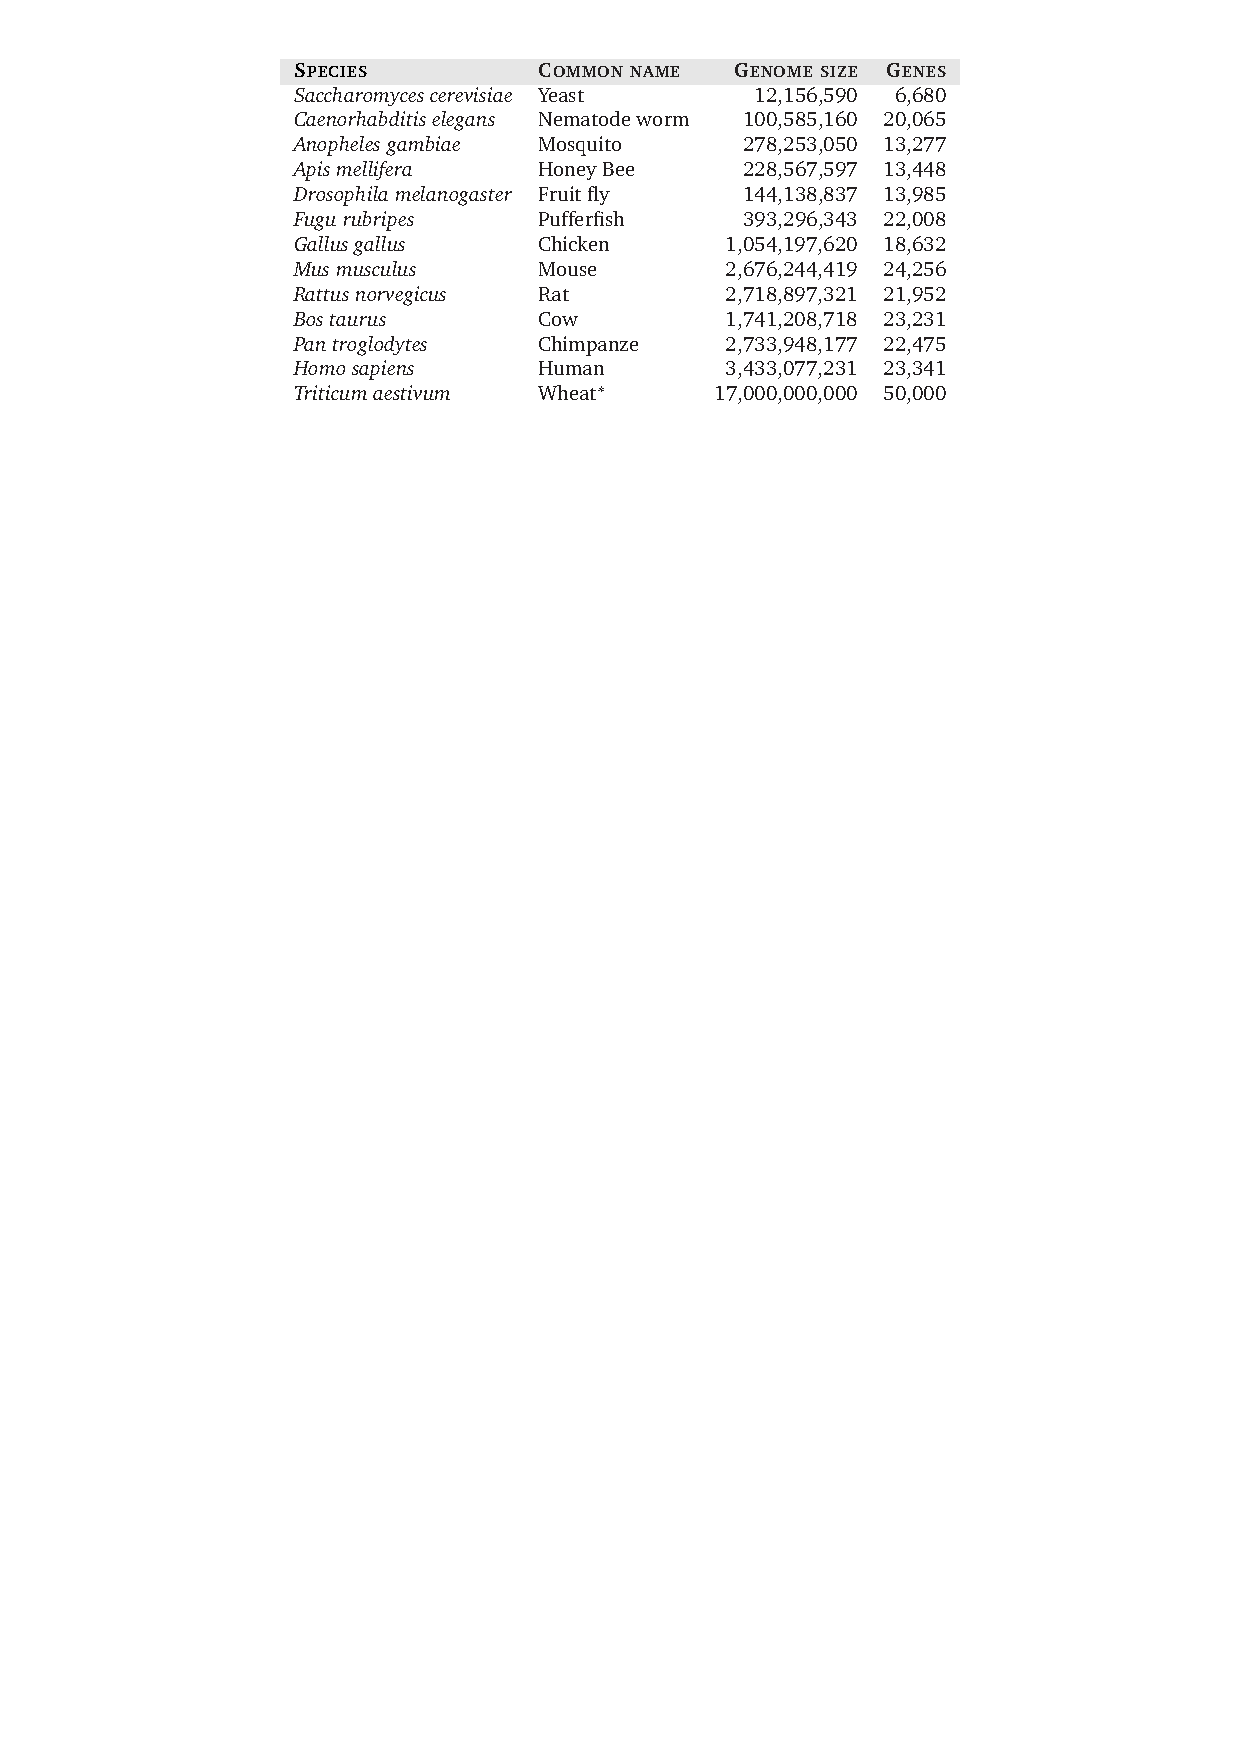
\includegraphics[bb=131 645 466 815,clip]{tables/gsizes}
\end{center}
\end{minipage}
\mycaption{tab:gsizes}% label
          {Comparison of the sizes of several eukaryotic genomes}% lof
          {Comparison of the sizes of several eukaryotic genomes.}% caption header
          {Data extracted from \ensembl{} (May, 2006). Estimated values for wheat.}
\end{center}
\end{table}

\noindent Broadly, bioinformatics tasks can be divided intro three categories:

\begin{menumerate}
\item
Implementation of databases to organize existing information from many areas of biological research
such as genomics, transcriptomics and proteomics, allowing the public scientific community to 
efficiently access the data and to avoid redundancy and multiplicity. Doubtlessly, the advent of 
internet has played a central role in the achievement of this challenge \citep{goodman:2002a}.
\item
Development of new algorithms and statistics that aid the analysis of the data such as sequence 
alignment methods, motif detection techniques, phylogenetic studies or protein folding simulation.
Advanced algorithmic methods and mathematical frameworks are essential to extract biological
knowledge from the databases.
\item
The analysis of such data and the interpretation of the results in a biologically meaningful 
manner to provide a more global perspective (new testable hypotheses) in future experimental designs. 
So far, it is far often easier to produce sequence data than to understand its function so that this 
is the most complicate of the three tasks \citep{bogusky:1998a,claverie:2000a,pearson:2001a}.
\end{menumerate}

\subsectionblue{Sequence databases}
\index{sequence!seqdb@databases} 

%%%%
% Figure 5: Genome composition 
%%%%
\begin{figure}[t!]
\begin{center}
\setlength{\fboxsep}{0pt}
\fbox{
\begin{tabular}{c}
\incgraph{width=0.6\linewidth}{ps/gcompo1}\\
\incgraph{width=0.6\linewidth}{ps/gcompo2}
\end{tabular}}
\mycaption{fig:gcompo}% label
          {The organization of the human genome}% lof
          {The organization of the human genome.}% caption header
          {(Top) A segment of the human genome.
           (Bottom) The contribution of different genomic elements to the human genome.
           Adapted from \citet{brown:1999a}.}
\end{center}
\end{figure}


A biological database is a large, organized body of persistent data designed to be queried
and retrieved in a very efficient manner by the scientific community. Because of the nature of the 
first data, ancient databases were merely collections of sequences of proteins distributed as a printed 
work \citep{dayhoff:1965a}. Nonetheless, the need for an electronic format became obvious just when the 
amount of sequences was unmanageable \citep{baxevanis:2005a,mount:2001a}. With substantial experimental 
sequencing improvements and the advent of DNA sequence databases initiated by the European Molecular 
Biology Laboratory (EMBL, Germany) and Los Alamos National Laboratory (LANL, United States), the 
number of available sequences experienced an exponential growth (see Figure \ref{fig:genbank}).

Major public nucleotide and protein sequence databases such as 
\embl{}
\index{EMBL} 
(\citealp{kulikova:2004a}, \webitemlink[embl]
    {\url{http://www.ebi.ac.uk/embl/}}
    {\db{European Molecular Biology Laboratory (EMBL)}}
    {%
      EMBL-nucleotide sequence database.
    }%
    {emblurl})
or \genbank{}\index{GenBank}\footnote{GenBank is now under the auspices of the National Center for Biotechnology Information (NCBI, United States).}
(\citealp{benson:2004a}, \webitemlink[genbank]
    {\url{http://www.ncbi.nlm.nih.gov/Genbank/index.html}}
    {\genbank{}}
    {%
       GenBank is the NIH genetic sequence database, an annotated 
       collection of all publicly available DNA sequences.
    }%
    {emblurl})
are repositories of sequences submitted by researchers in order to make them accessible for the
rest of the biological community. An accession number and a set of annotations are provided for
each sequence entry. Using flat files as a standard format, the features of each sequence are displayed 
in a simple format that divides each line of information into two elements: a field descriptor and a 
value. The popular \prog{FASTA} format 
\index{FASTA!fformat@format} 
is one of the \emph{de facto} standards that have been 
adopted to represent a sequence of nucleotides or amino acids (see Figure \ref{fig:gbentry} for an
example of a GenBank entry and the associated \prog{FASTA} file).

%%%%
% Figure 6: growth of genbank (web)
%%%%
\begin{figure}[t!]%
\begin{center}
\setlength{\fboxsep}{0pt}
%\fbox{
\incgraph{width=0.5\linewidth}{ps/gbgrowth}%}
\mycaption{fig:genbank}% label
          {Growth of the \genbank{} (1982-2004)}% lof
          {Growth of the \genbank{} (1982-2004).}% caption header
          {Adapted from \genbank{} (\webitemlink[genbank-stats]
    {\url{http://www.ncbi.nlm.nih.gov/Web/GenBank/genbankstats.html}}
    {\genbank{}}
    {Overview about the content of \genbank{}.}
    {genbankstatsurl}).}
\end{center}
\end{figure}

Because of the relative lack of control over the quality and quantity of the data stored in the 
sequence databases during the first years, there was soon a necessity to maintain collections of data
free of redundancy and errors constructed from the original repositories. Since then, numerous curated 
databases, also known as secondary databases, have appeared aiming to avoid any type of multiplicity and 
low quality data \citep{baxevanis:2005a}. 

%%%%
% Figure 7: Genbank entry
%%%%

\begin{figure}[t!]
\begin{center}
\setlength{\fboxsep}{0pt}

\begin{tabular}{cc}
\rotatebox{90}{\genbank{}} & 
\fbox{\begin{tabular}{c}
\incgraph{width=0.575\linewidth}{ps/gbentry1}\\
\incgraph{width=0.575\linewidth}{ps/gbentry2}
\end{tabular}}\\
& \\
\rotatebox{90}{\prog{FASTA}} & 
\fbox{\begin{tabular}{c}
\incgraph{width=0.575\linewidth}{ps/gbentry3}
	  \end{tabular}}
\end{tabular}
\mycaption{fig:gbentry}% label
          {An example of \genbank{} entry}% lof
          {An example of \genbank{} entry and a \prog{FASTA} sequence.}% caption header
          {}
\end{center}
\end{figure}

A successful example of these refined catalogues is the \refseq{} 
\index{RefSeq} 
collection (\citealp{pruitt:2005a},
\webitemlink[refseq]
    {\url{http://www.ncbi.nlm.nih.gov/RefSeq/}}
    {\db{The Reference Collection (RefSeq)}}
    {%
      The Reference Sequence (RefSeq) collection aims to provide a comprehensive, 
	  integrated, non-redundant set of sequences, including genomic DNA, transcript (RNA), 
	  and protein products, for major research organisms.
    }%
    {refsequrl}).
The major goal of this database is to provide a unique sequence for each molecule in the protein
synthesis pathway (DNA, mRNA and protein). To reduce the noise produced by the representation of 
a single biological entity with many entries in the sequence databases, each biological entity is 
represented only once in \refseq, maintaining a non-redundant repository.

\subsectionblue{Genomic databases}
\index{genome!gdb@databases}

Once the complete assembly of first eukaryotic genomes such \Scer{} \citep{goffeau:1996a} or 
\Dmel{} \citep{adams:2000a} was achieved, the principal focus of computational biology research 
shifted from individual sequences to chromosomes and whole genomes. With the release of the human 
genome \citep{lander:2001a,venter:2001a,ihgsc:2004a}, it became necessary to introduce an important 
change in the way the assemblies and the genome annotations were presented. \index{genome!genrelease@projects} 
Finally, the recent availability of the mouse genome \citep{waterston:2002a}, the chicken 
genome \citep{hillier:2004a} 
and the sequencing of other model organisms has augmented the need for a new kind of tools to permit 
the annotation and comparison of many genomes in a more sophisticate form. In addition, support for 
genomes that have not been finished yet has also been crucial (archives of traces and preview releases).

\noindent There are three well established genome browsers that aim to fulfill this need:

\begin{mitemize}
\item
The \ensembl{} project \index{Ensembl} 
(\citealp{birney:2004a}, \webitemlink[ensembl genome browser]%
    {\url{http://www.ensembl.org/}}%
    {\ensembl{}}%
    {%
%%
    Ensembl is a joint project between EMBL - EBI and the 
	Sanger Institute  to develop a software system which produces 
	and maintains automatic annotation on selected eukaryotic genomes.
%%
    }%
    {ensemblurl}), %
a collaboration between the European Bioinformatics Institute and the Sanger Institute.
The main browser currently provides a set of gene, transcript and protein predictions for each
genome. Data is presented on pages called Views, each View showing a different level of detail.

\item
The \ucscgb{} \index{UCSC genome browser} 
(\citealp{karolchik:2003a}, \webitemlink[ucsc genome browser]%
    {\url{http://genome.ucsc.edu/}}%
    {\ucscgb{}}%
    {%
%%
	  This site contains the reference sequence and working draft assemblies for a 
	  large collection of genomes. It also provides a portal to the ENCODE project.
%%
    }%
    {ucscgburl}), %
produced by the University of California, Santa Cruz Genome Bioinformatics Group. 
It serves annotations for many eukaryotic genomes, presenting the information in the 
form of tracks. Each track corresponds to a certain genomic feature. 

\item
The \ncbimv{} 
(\citealp{wheeler:2005a}, \webitemlink[ncbi map viewer]%
    {\url{http://www.ncbi.nlm.nih.gov/mapview/}}%
    {\ncbimv{}}%
    {%
%%
    The Entrez Map Viewer is a software component of Entrez Genomes. It allows you to 
	view an organism's complete genome, integrated maps (when available) for each chromosome, 
	and sequence data for a region of interest.
%%
    }%
    {ncbigburl}), %
provides maps for a lot of organisms, many of them without finished assembly. The browser 
is tightly linked to most services of the NCBI web. The information is displayed using  
maps. Maps are vertical representations of annotations along a given chromosome. There is a 
map associated to each genomic feature.

\end{mitemize}

The core of the three browsers is the internal gene annotation pipeline that must be executed on
every new sequence assembly of each genome. Genes are annotated according to experimental 
evidence and computational predictions. Comparisons between different genomes are also employed to 
improve the results. Moreover, other genome features such as regulatory regions, repeats, transcripts
or sequencing markers are integrated with the sequence and the annotated genes. In Figure 
\ref{fig:gbrowsers}, a screenshot of the same gene displayed in the \ucscgb{} and \ensembl{} is shown.

%%%%
% Figure 8: Genomic browsers
%%%%
% GBROWSERS: 
\begin{figure}[t!]
\begin{center}
\setlength{\fboxsep}{0pt}
\begin{tabular}{cc}
\rotatebox{90}{\centering\ucscgb{}} & \fbox{\incgraph{width=0.9\linewidth,height=8.75cm}{ps/gbrowsers1}}\\
 & \\
\rotatebox{90}{\centering \ensembl{}}& \fbox{\incgraph{width=0.9\linewidth,height=8.75cm}{ps/gbrowsers2}}
\end{tabular}
\mycaption{fig:gbrowsers}% label
          {The human URO-D gene in the \ucscgb{} and \ensembl{}}% lof
          {The human URO-D gene in the \ucscgb{} and \ensembl{}.}% caption header
          {}
\end{center}
\end{figure}


\subsectionblue{Data integration (integromics)}

The biological information that can be now accessed in the databases has not been generated
during a continuous process with several steps following an increasing order of complexity. On the 
contrary, different and discontinuous waves of genome-wide data have overlapped to form the current
body of knowledge. The new high-throughput technologies that have arisen in the last decades have
been the main catalyst conducing the progress. The first wave was the large-scale production of 
fragments of transcripts also named expressed sequence tags (ESTs). \index{ESTs}
The second wave was originated by
the sequencing of whole microbial organisms and was quickly followed by the achievement of the genomic
sequence of many eukaryotic organisms including human. Simultaneously, microarrays and
related technology have produce an overwhelming amount of expression data for which new analysis 
methods are still being designed \citep{searls:2000a}. 

In the near future, new waves of information are expected, such as the generation of maps of 
functional SNPs (see section \ref{sec:pgera}), or the complex interaction networks produced by 
emerging systems biology \citep{kitano:2002a}. Information technologies have adapted to the changing
nature of the new data. With every explosion of new knowledge, previous procedures have been reused 
and others have been created from scratch to integrate the new type of data with the already 
existing information. The power of data integration arises not from the value of every separate kind of 
information but from the gain produced by the fusion of all of them. With the advent of more
waves of knowledge, integromics will become absolutely essential to manage an amount of 'Omic' 
information that will exceed exabyte ($10^{18}$ bytes) quantities \citep{searls:2005a}.

Biological databases are essential resources used by biologists around the world. However, each one
contains only a subset of biological knowledge. This specificity increases the complexity of finding 
the answer for the majority of questions. Thus, several databases must be explored in order to obtain
the expected results. Cross-database queries require complex mechanisms of data integration that are
often not implemented properly \citep{stein:2003a}. 

For instance, the name of biological objects such as genes in the genomic browsers of several species 
(e.g. Rad24, rad24 or RAD24) or the definition of simple entities such as the gene concept 
(considering only transcript or transcript and regulatory region) can be a source of disagreement. 
Consequently, the role of ontologies to facilitate data integration must not be neglected. The 
popular \go{} \index{Gene Ontology (GO)}
(\citealp{tgoc:2000a}, \webitemlink[gene ontology]%
    {\url{http://www.geneontology.org}}%
    {\go{}}%
    {%
%%
	 The Gene Ontology (GO) project is a collaborative effort to address the need for consistent 
	 descriptions of gene products in different databases. The Gene Ontology project provides a 
	 controlled vocabulary to describe gene and gene product attributes in any organism.
%%
    }%
    {gourl}) 
establishes a taxonomy of controlled vocabulary that is used by most genome annotation projects
to uniformly annotate the function of genes.

\noindent There are several ways in which databases developers have tried to integrate databases:
\begin{mitemize}
\item
Link integration. Hypertext links are used to jump from one database to another. Although it is
the most popular solution, it has two severe drawbacks: links are vulnerable to name ambiguities and 
their updating is laborious.
\item
View integration. An environment around the databases is built to create the illusion of a unique
resource formed by different sources of data with specific data drivers to retrieve the information. 
The complexity of such a design is the main disadvantage of this strategy.
\item
Data warehousing. Merge all of the databases into a single database. Due to the continuous updating
of biological databases and the impossibility of reusing the software from one release to the next,
this approach is unfeasible in practice.
\end{mitemize}

%%%%%%%%%%%%%%%%%%
\sectionblue{The post-genomic era}\label{sec:pgera}

\subsectionblue{New forms of investigation}

The availability of many genomes and the improvement of very large-scale gene expression experiments
have substantially modified the form in which current research is focused \citep{searls:2005a}. 
The classical hypothesis-driven research paradigm, in which a specific proposition is addressed over 
a set of targets, is progressively being substituted with data-driven investigations, in which high-throughput 
explorations are performed typically over the whole collection of genes of an organism to detect
previously unknown relationships. Data-diving excursions have several risks derived from their 
massive exploration. Correct normalization and replication of the results is extremely difficult.
In addition, there is usually a high probability of finding pure artefactual relations due to the 
low signal/noise ratio observed in such experiments \citep{searls:2005a}.

Much effort must be invested to make bioinformatics become part of the wet-dry cycles of research
\citep{searls:2000a}. Such discovery processes occur whenever a computational method is linked to a 
biological one, such that predictions from the former can be tested at the bench, within a feedback 
strategy. Once the computational candidates have been delivered, they should be monitored during the 
experimental pipeline, using such results to refine the original computational model \citep{searls:2000a}.

\subsectionblue{Genomics and health}

Virtually every human illness has a hereditary component \citep{collins:2001a}. The characterization 
of the genetic determinants of disease would provide remarkable opportunities for clinical medicine. 
Current clinical practice is still based on phenotypic criteria to define most diseases rather than
studying the underlying mechanisms. Obtaining the sequence of the human genome is only the end of the 
beginning \citep{collins:2001a}. Among the grand challenges to achieve after the sequence of many
genomes is available is the development of strategies for identifying the genetic contributions to 
disease and the gene variants that promote good health and resistance to disease \citep{collins:2003a}. 
Progress is slow but evidence suggests that while public health and antibiotics have played the major 
roles in the past 50 years, the next 50 are likely to belong to genetics and molecular medicine 
\citep{bell:2003a}.

Simple changes in our genes can lead to disease. 
\index{gene!geneillness@genes and illness}
Single gene mutations, which are already commonly 
used in diagnostic practice (genetic and disease markers), cause approximately $6,000$ inherited 
diseases also known as monogenic diseases. Disorders like cystic fibrosis, anemia or hemophilia 
affect millions of people worldwide. For more common diseases such as heart disease, diabetes, or 
Alzheimer's disease, the interplay of multiple genes and multiple non-genetic factors (environment 
effects) that contribute to disease susceptibility is still being characterized (GSK report: Genes 
and diseases, \webitemlink[gsk]%
    {\url{http://genetics.gsk.com/link.htm}}%
    {Genetics GSK report: Genes and diseases}%
    {%
%%
    GlaxoSmithKline educational resource.
%%
    }%
    {gskurl},
NHGRI/NIH report: Genetics, the Future of Medicine, \webitemlink[nhgri]%
    {\url{www.nhgri.nih.gov}}%
    {NHGRI/NIH report: Genetics, the Future of Medicine}%
    {%
%%
    National Human Genome Research Institute.
%%
    }%
    {nhgriurl}).

For example, loss of control in the growth mechanisms of cells results in cancer. 
\index{cancer} \index{gene!gcancer@cancer}
The transformation of a normal cell into a cancerous one is caused by molecular changes that underly
growth-signal independence, insensitivity to anti-growth signals, evasion of immunosurveillance,
apoptosis evasion, unlimited replicative potential, tissue invasion and metastasis. 
These molecular changes involving several genes can be produced by certain
events that alter the genome such as point mutations, gene amplifications and deletions, and 
chromosomal translocations. The intimate relationship between cancer and genome sequencing projects
has originated the recent launch of several cancer genome projects \citep{strausberg:2003a}.

%%%%
% Figure 9: Classes of SNPs
%%%%%
\begin{figure}[t!]%
\begin{center}
\setlength{\fboxsep}{0pt}%
%\fbox{
\begin{tabular}{cc}
\incgraph{width=0.25\linewidth,height=6cm}{ps/snp1} &
\incgraph{width=0.25\linewidth,height=6cm}{ps/snp2}\\
\end{tabular}%}
\mycaption{fig:snps}% label
          {Using SNPs to locate susceptibility genes}% lof
          {Using SNPs to locate susceptibility genes.}% caption header
          { (Left) SNP profiling of two groups of people.
            (Right) Categories of SNPs according to their location.
            Adapted from GSK report: Genes and diseases.}
\end{center}
\end{figure}%

\subsectionblue{Pharmacogenomics}
\index{pharmacogenomics}

Before the end of this century, shortly after a person is born, her genotype will be saved at her 
physician's office to record the presence  or absence of specific variations known to be relevant 
for assessing disease susceptibility and prediction response to drug types. Biomolecular profiling 
throughout her life will complement this information to provide recommendations about life-style 
or diet and to detect early stages of a disease. This future scenario in which personalized medicine
and therapy are present in our lives to increase the quality of life and life-span is not 
unrealistic \citep{sander:2000a}. 

In 1998, adverse drug reactions produced over $100,000$ deaths in the United States, being one of the
leading causes of hospitalization and death. The one-size-fits-all formula typically works for only 
$60$\% of the population at best. The way a person responds a drug (positively or negatively) 
is a complex trait influenced by many different genes. Pharmacogenomics \footnote{The related term 
pharmacogenetics appeared in the 1950s describing the study of inherited genetic variation in drug 
metabolism and response.} is the science that examines the gene variations that dictate drug response
and explores how to use them to predict whether a patient will have a good reaction, a bad reaction
or no reaction to a given drug 
(\citealp{evans:1999a}, NCBI report: pharmacogenomics,
\webitemlink[ncbi a science primer pharmacogenomics]
    {\url{http://www.ncbi.nlm.nih.gov/About/primer/pharm.html}}
    {\db{NCBI} A Science Primer (pharmacogenomics)}
    {%
      A Basic Introduction to the Science Underlying NCBI Resources.
    }%
    {ncbiinfothreeurl}).

First studies focused on the broadest categories of inheritance: ethnicity, geography, language and
race. Several SNPs mapping projects are working to provide a catalogue of observed 
one-letter differences between individuals in a population. SNPs are present throughout
\index{SNP!SNPdis@distribution} 
the human genome with an average frequency of $1$ per $1,000$ base pairs. Their relatively even 
distribution make them valuable as genetic markers. To be helpful, the polymorphism must be shared 
by at least $1$\% of the population tested, thus becoming a shared SNP. Mutations are less
common differences, occurring in a smaller proportion.

With these SNP maps, genetic profile comparison of patients who may suffer from serious side effects 
and those that may not, might be useful to detect one or more SNPs that differ between both groups. Careful 
examination of the small area of the genome where the differences are found will classify them
into functional and non-functional SNPs (see Figure \ref{fig:snps}). 
\index{SNP!SNPclas@classes} 
For instance, SNPs found in 
protein coding regions (cSNPs) would be good candidates to elaborate a hypothetic explanation of
the observed drug response as long as they produce a change in the translated amino acid sequence 
(non synonymous changes).

The haplotype is the set of closely related genes (alleles) that tend to be inherited together as 
a single unit. \index{haplotype} 
The International HapMap Project is currently in charge of developing the haplotype 
map of the human genome \citep{tihc:2003a}. The official repository of SNPs mined by this project
is the NCBI \dbsnp{} database
(\webitemlink[dbSNP]%
    {\url{http://www.ncbi.nlm.nih.gov/SNP/}}%
    {\dbsnp{}}%
    {%
%%
     The NCBI database of SNPs.
%%
    }%
    {dbsnpurl}) %% 
that contains information for other genomes as well. SNP annotation is also integrated in the 
genomic browsers explained in Section \ref{sec:gera}. For further information about sequence
polymorphisms, see \citet{mullikin:2005a}.

%%%%%%%%%%%%%%%%%%
%%% References for this chapter
%%% ENCERRAR ENTRE LLAVES PARA EVITAR PROBLEMAS
\bibliographystyle{plainnat}
{\bibliography{sections/bibliography}}
        % Introduction about biology and bioinformatics
    \clearemptydoublepage

%%% BLOCK 2
\partorange[State of the Art]{\textbf{S}tate of the Art}

    %%%%%%%%%%%%%%%%%%%%%%%%%%%%%%%%

% The golden age of sequence analysis

%%%%%%%%%%%%%%%%%%%%%%%%%%%%%%%%

\chapter[The golden age of sequence analysis]{\textbf{T}he golden age\\of sequence analysis}\label{sec:algorithms}
\sectionorange*{Summary}
\begin{center}
\begin{tabular}{c}
\fcolorbox{blue}{verylightgrey}{
\begin{minipage}[][4cm][c]{0.8\linewidth}
\sffamily
%abstract 
This chapter aims to be a historical survey of the sequence comparisons algorithms analyzing the most 
relevant solutions. The algorithms that represented innovative changes in the field are described in detail,
covering the concepts of global, local and multiple alignment of sequences. In addition, the theoretical 
framework of the map alignment problems necessary to understand the rest of work presented in this thesis 
is also formalized here.
\end{minipage}}\\
\\[2ex]
\begin{minipage}[][4cm][c]{1.1\linewidth}
\minitoc
\end{minipage}
\end{tabular}
\end{center}
\newpage



\sectionorange{Foundations of sequence comparison}\label{sec:history}

\lettrine[lines=4,loversize=-0.1,lraise=0.1,lhang=.2]{T}{he topic of biosequence comparison} has a rich 
history dating back over 40 years. It is certainly very difficult to trace a line in some moments to 
establish the order in which every new development was presented because of the enormous body of
publications that have contributed substantially to improve this field. Several general reviews have been 
used to reconstruct the history of biological sequence comparisons 
\citet{mount:2001a,myers:1991a,ouzounis:2003,sankoff:1983a,meidanis:1997a, waterman:1984a}. 

Molecular evolution began to be studied in the 1960s when a few protein sequences were available, being
published into the protein sequence atlas \citep{dayhoff:1965a}. Soon, pioneering analysis appeared to 
infer the evolutionary relationships from these sequences, depicted as distances in phylogenetic trees 
\citep{fitch:1967a}. 

Outside the molecular biology, other significant advances in mathematics and in the emerging discipline of
computer science contributed decisively to the current state of the art. For instance, it is impossible to 
understand the history of modern sequence alignment without mentioning the birth of a new technique in the
1950s to solve multistage decision process problems called dynamic programming \citep{bellman:1957a,dreyfus:2002a}. 
A problem is solved by dynamic programming if the answer can be efficiently determined by computing a table of 
optimal answers to progressively larger subproblems. The principle of optimality requires that the optimal answer 
to a given subproblem is expressible in terms of optimal answers to smaller subproblems. During all this time, 
despite innumerable optimal and heuristic approaches have been proposed to obtain the best alignments between 
two sequences with the minimum cost, dynamic programming is still the most stable technique to solve the original 
problem and many of its variations.

Another key concept is the definition of several metrics of distance between sequences in the coding 
theory field. Since noise in a transmission channel introduces errors into the signal reception, several
mechanisms were developed for detection and correction of such errors. The Hamming distance, defined as the 
number of positions in which two sequences differ, was oriented to detect only substitutions \citep{hamming:1950a}. 
Next, \citet{levhenshtein:1966a} presented the edit distance, which was the earliest known use of a distance 
function that is appropriate to detect insertions and deletions of symbols in the original message.
 
It is not clear when the basic dynamic programming algorithm for molecular sequence comparison first 
appeared. It was probably rediscovered many times in different contexts. The well-known paper by
\citet{needleman:1970a} who presented an algorithm for maximizing the number of matches minus the number
of insertions and deletions is generally considered to be the first important contribution. Although no 
complexity analysis was provided, the original \citeauthor{needleman:1970a} algorithm measured the
homology between two sequences in a $O(n^3)$ time.

A more rigorous approach with solid mathematical foundations arised from the problem of computing the 
distance between two sequences \citep{ulam:1972a,beyer:1985a}. \citet{sellers:1974a} presented a dynamic
algorithm based on the Levhenshtein metric distance. Though less flexible for future variations of the 
problem, this new approach fitted better with the perspective of evolutionary distance analysis 
developed earlier. Under the realistic assumption that both sequences have $n$ nucleotides, the 
\citeauthor{sellers:1974a} algorithm have computation time proportional to $O(n^2)$. A comprehensive 
study of equivalence between similarity and distance was presented in \citet{smith:1981b}. 

Within the field of computer science, sequence comparison appeared in simpler incarnations of the 
molecular biology problems, for comparing the contents of files or correcting the spelling of words. For example, 
the longest common subsequence problem (LCS) consists on finding an alignment that maximizes the number of
identical aligned pairs between two sequences (see \citet{apostolico:1987a} for a review).
Interestingly for long sequences, \citet{hirschberg:1975a} applied the divide and conquer strategy to 
solve the LCS problem in $O(2 n^2)$ time with a linear space cost instead of the established quadratic cost.
\citet{myers:1988a} generalized this technique to align two sequences using $O(n)$ space.

Nonetheless, the treatment of gaps was still biologically unrealistic as a deletion of $n$ symbols and $n$ 
deletions of one symbol were punished indistinctly. \citet{waterman:1976a} accommodated the same 
algorithm to deal with multiple deletions and insertions, introducing the concept of general gap 
penalty functions. \citet{gotoh:1982a} reduced the asymptotic cost from $O(n^3)$ to $O(n^2)$, under the
application of the affine gap penalty functions in which there was an initial penalty for opening a gap 
and an additional minor penalty for extending an existent one. Apart from general and affine gap functions, 
\citet{waterman:1984a} introduced the concept of concave gap function in which the cost of extending an 
existent gap grows with the logarithm of the length of the gap as a continuous curve. Later, \citet{eppstein:1988a} 
and \citet{miller:1988a} independently arrived at $O(n^2 \log{n})$ solutions of the problem.

DNA and protein sequences are the result of an evolutionary process that tend to preserve those
parts that are key to perform a function, permitting variation in the rest. Thus a global comparison
can easily produce a very poor alignment of two sequences that have some parts in common while others
are completely free of conservation. \citet{smith:1981c} introduced the concept of local alignment
with a simple variation in the basic global similarity algorithm without increasing its cost. Under the 
premise of a negative gap penalty, reported alignments are regions of high similarity with a positive 
score within. \citet{sellers:1984a} tried to export the same concept to the distance metric. Only, those 
paths in the matrix whose density of mismatches was below a certain threshold were reported.

Thousands of genomic and proteomic sequences, that is millions of nucleotides and amino acids,
are rapidly being accumulated in the biological databases. However, searching a database with a query 
sequence for similarities to other sequences using the optimal algorithms enumerated above
is clearly unfeasible when this simple operation involves thousands of comparisons between two sequences.
To overcome this problem, a new family of heuristic procedures that produce nearly correct answers in
a simple and cheaper fashion was designed. The most popular representatives of these are the program
FASTA \citep{pearson:1988a} and the program BLAST \citep{altschul:1990a}. The FASTA heuristic is based
on identifying the identities between two sequences (diagonals in the matrix) and then applying 
some more expensive procedures only on those subalignments. BLAST processing relies on first, detecting
ungapped segment pairs of high score and then, extending them from both ends until a threshold value
is reached. 

A collateral effect of producing hundreds of alignments was the concern about the quality of a
given alignment between two sequences. The significance of a local alignment score can be tested by 
comparing with the distribution of scores expected by aligning two random sequences with the same length 
and composition \citep{karlin:1990a}. These random sequence alignment scores follow a distribution called
the extreme value distribution (also known as the Gumbel distribution), which is similar to a normal
distribution but with a positively skewed tail in the higher score \citep{gumbel:1962a}. Less interest 
has traditionally been focused on global comparisons because of a global alignment is always produced by 
definition even between random or unrelated sequences, growing the score proportionally to the length of 
them.

In attempt to distinguish more distant relationships, the implementation of comparisons for more than 
two sequences is the logical evolution to locate elements with function that are conserved for instance 
in several homologous sequences.
\citet{waterman:1976a} naturally extended the basic dynamic programming recurrence for $k$ sequences, with
an exponential cost $O(n^k)$. As this approach is generally impractical, some heuristics
appeared to solve the problem with a minor cost. The most popular of them is the hierarchical or 
clustering method called progressive alignment that first takes $O(k^2 n^2)$ to perform all pairwise 
alignments and second, produce a multiple alignment following a guide tree to merge these alignments 
\citep{feng:1987a}. The program CLUSTALW \citep{thompson:1994a} combines this strategy with different 
weighting schemes according to the progression in the distances tree. Previously, \citet{carrillo:1988a} 
developed another method based on identifying the projections of the pairwise alignments that can form the multiple 
alignment. Moreover, hidden Markov models have been used to produce multiple alignments of a family of
sequences to which more members can be dynamically be added (profile HMMs, see \citealp{durbin:1998a}).

Pattern discovery and local multiple sequence alignment have been very closely related problems 
\citep{brazma:1998a}. For instance, a conserved pattern or a block of ungapped common motifs in a set of 
sequences defines a local multiple alignment. In any case, the problem is even more difficult than pure 
global alignment and optimal approaches were discarded beforehand. Some heuristic approaches have been 
proposed to circumvent the complexity. Iterative methods do not necessarily find the best pattern, but may
converge to a local maximum. Gibbs sampling \citep{lawrence:1993a} and expectation maximization
\citep{bailey:1994a} are successful examples of these stochastic techniques.

Some pattern recognition problems are too complex or too ambiguous to be expressed as a simple pattern
matching operations over a sequence. In these cases, a richer environment over the basic sequences is 
needed to describe the comparison of such elements \citep{knight:1995a}. For example, for most sequence
comparison problems there is a corresponding map comparison algorithm. Map comparisons were introduced
to model the alignment of restriction enzyme maps. These were used in the construction of physical maps 
prior to genome sequencing projects. The basic definition of the problem by \citet{waterman:1984c} 
contained an $O(n^4)$ time cost algorithm although it was noticed the dynamic programming matrix was 
very sparse. Later, \citet{myers:1992a} improved the time efficiency by using an analytical approach
that reduced the cost to $O(n^2 \log{n})$. Additional refinements of the problem produced new algorithms 
to deal with map data errors \citep{huang:1992a} or to align specifically short maps to longer ones 
\citep{miller:1990a}.

Not only analytical approaches have been employed for comparing sequences. Dot matrix comparisons, also
known as dotplots, are visual comparisons that can be useful to conduct afterwards a deeper research with dynamic 
programming algorithms only on those conserved regions \citep{gibbs:1970a}. Sequence logos are graphs
that illustrate the amount of information in each column of an alignment or motif \citep{schneider:1990a}. 

Sequence comparison algorithms that were developed to solve biological problems have been recreated and 
applied in other scientific fields \citep{sankoff:1983a}. For instance, applications can be found in geology 
(stratigraphic sequences), in dendrochronology (time dating based on tree rings), or in bird song recognition 
(animal communication). 


\sectionorange{Alphabets, sequences and alignments}\label{sec:}

\subsectionblue{Biological significance of sequence comparison}

\index{sequence!seqbs@evolution}
Gene evolution is thought to occur by
gene duplication, creating two tandem copies of the gene in a given ancestor species. In rare 
cases, new mutations in one of the copies can provide an advantageous change in function. The two 
copies then evolve along separate pathways. At a certain evolutionary point, a speciation event 
gives rise to two separate branches (two new species) of the tandem gene preserving a similar 
sequence due to the single gene ancestor (see Figure \ref{fig:phylogeny}). The four copies of the 
original gene are said to be homologous: \index{gene!hom@homology} \index{homology}
the two corresponding units of the tandem gene in each species are orthologous 
\index{gene!ort@orthology} \index{orthology} while the two units of each tandem gene in the 
same species are paralogous. \index{gene!paral@paralogy} \index{paralogy}
Molecular evolution events include substitutions of one nucleotide or amino acid for another as well
as insertions and deletions (indels) of others. More complex genetic rearrangements such inversions,
transpositions, translocations or duplications can shuffle larger parts of the genes or of the proteins, 
producing chimeric products in which some regions are homologous and others are not \citep{mount:2001a}.

Sequence comparison 
\index{sequence!seqcmp@sequence comparison}
consists of finding which parts of the sequences are alike and which parts differ.
This operation is extremely useful for discovering functional, structural and evolutionary 
information in biological sequences. If two sequences from different organisms are similar, there may 
have been a common ancestor sequence that would make these sequences to be homologous. Phylogenetic analyses
are usually conducted starting from multiple sequence comparisons, and then producing hierarchical trees that 
would explain the evolution of the species.


\subsectionblue{Alphabets and sequences}\label{subsec:alphabets}

A finite alphabet 
\index{alphabet}
is a set of symbols or characters. For instance, the four-letter DNA and RNA 
alphabets are defined as:
\begin{center}
\fcolorbox{white}{verylightgreen}{
\begin{minipage}[][][c]{0.95\linewidth}
\begin{center}
$\Sigma_{DNA} = \{ \mbox{A}, \mbox{C}, \mbox{G}, \mbox{T}\}$ and $\Sigma_{RNA} = \{ \mbox{A}, \mbox{C}, \mbox{G}, \mbox{U}\}.$
\end{center}
\end{minipage}}
\end{center}
To support some degree of variation or ambiguity in a symbol, the IUPAC extended genetic alphabet 
\index{alphabet!iupac@IUPAC alphabet}
of 15 elements allows for special symbols possessing multiple letters (see Table \ref{tab:code1}).
The single-letter amino acid alphabet contains 20 elements \footnote{Nowadays, new amino acids are
still being unveiled such as Selenocysteine.} from which all proteins are built (see Table 
\ref{tab:code2}).

$\Sigma^*$ denotes the set of all finite sequences of characters from $\Sigma$ including the empty 
sequence $\lambda$. A generic sequence $S$ of length $|S|=n$ symbols over a finite alphabet $\Sigma$ is 
\index{sequence}
defined as:
\begin{center}
\fcolorbox{white}{verylightgreen}{
\begin{minipage}[][][c]{0.95\linewidth}
\begin{center}
$S = s_1 s_2 \ldots s_n$ where $\forall i: 1 \leq i \leq n: s_i \in \Sigma$.
\end{center}
\end{minipage}}
\end{center}

A subsequence of $S$ between positions $i$ and $j$ of $S$ is the contiguous series of elements between 
\index{subsequence}
both positions\footnote{As defined in computer science, subsequences are subsets of characters of $S$
possibly not contiguous but arranged in their original relative order.}. If $i = 1$, the subsequence is called a 
prefix of $S$. If $j = n$, the subsequence is a suffix:
\begin{center}
\fcolorbox{white}{verylightgreen}{
\begin{minipage}[][][c]{0.95\linewidth}
\begin{center}
$S_{i,j} = s_i \ldots s_j$ where $1 \leq i \leq j \leq n$ and $\forall k: i \leq k \leq j: s_k \in S$.
\end{center}
\end{minipage}}
\end{center}


%%%%
% Figure 1: Phylogenetic relationships
%%%%
\begin{figure}[t!]
\begin{center}
\setlength{\fboxsep}{0pt}
\fbox{\incgraph{width=0.6\linewidth}{ps/homology}}
\mycaption{fig:phylogeny}% label
          {Gene evolution events}% lof
          {Gene evolution events.}% caption header
          {}
\end{center}
\end{figure}

\subsectionblue{Sequence alignments}\label{subsec:alignments}

Given two sequences $A = a_1 a_2 \ldots a_m$ and $B = b_1 b_2 \ldots b_n$ in a finite alphabet 
$\Sigma$, a sequence alignment 
\index{sequence!aln@alignment} \index{alignment}
of $A$ and $B$ is a correspondence $C$ between the symbols from the two
sequences 


\begin{center}
\fcolorbox{white}{verylightgreen}{
\begin{minipage}[][][c]{0.95\linewidth}
\begin{center}
\shortstack{$C(A,B) = \{ (a_{i_1},b_{j_1}),(a_{i_2},b_{j_2})\ldots(a_{i_T},b_{j_T})\}$ where\\
$1 \leq i_1 \leq i_2 \leq \ldots i_T \leq m, 1 \leq j_1 \leq j_2 \leq \ldots j_T \leq n$}
\end{center}
\end{minipage}}
\end{center}
such that:
\begin{menumerate}
\item
Each $a_k$ (or $b_l$) not appearing in the subsequence $a_{i_1} \ldots a_{i_T}$ (or $b_{j_1} \ldots b_{j_T}$)
is considered to be an insertion in the other sequence (or a deletion in this one).
\item
If the pair $(a_i,b_j) \in C \Rightarrow \forall k: b_k \in B \wedge k \neq j: (a_i,b_k) \notin C$
(one symbol only matches another symbol at most).
\item
If the pairs $(a_i,b_j),(a_k,b_l) \in C$ and $i<k \Rightarrow j<l$ (no inversions are allowed).
\end{menumerate}

For example, a possible alignment of the sequence $A=AAGTTC$ and the sequence $B=AGCCC$ is
\index{alignment!exam@example}
\begin{center}
\fcolorbox{white}{verylightgreen}{
\begin{minipage}[][][c]{0.95\linewidth}
\begin{center}
\begin{tabular}{ccccccc}
$A = $ & A & A & G & T & T & C\\
& | &  & | &  &  & | \\
$B = $ & A & -- & G & C & C & C.\\
\end{tabular}
\end{center}
\end{minipage}}
\end{center}

\index{alignment!combis@changes}
This alignment represents a certain hypothesis about the evolution of the two sequences 
\citep{waterman:1990a}: three of the nucleotides have not changed since the common ancestor of $A$ 
and $B$ (matches), there have been at least two substitutions (mismatches), and one nucleotide has 
been either inserted or deleted (a gap), which is denoted with the symbol ``--''.

\index{alignment!score@scoring function}
If we adopt a scoring function that assigns a given value to a match, a mismatch and a gap, every 
column of the alignment will receive a score and the total score of the alignment will be the sum
of the values assigned to its columns. The best alignment will be the one that optimizes the total 
score. In the literature, two different types of measures have been devised to construct such a scoring 
function : similarity and distance (see \citet{smith:1981a} for a review).

\subsubsectionblue{Sequence similarity}
\index{similarity} \index{sequence!sim@similarity}
Similarity is a measure of how alike two sequences are. An alignment is scored by rewarding the
identities and in less degree, the substitutions, and punishing the gaps. 

Let $(a_i,b_j)$ be a match (or a mismatch) of type $k$ with a weight $\alpha_k$ and let $w_l$ 
be the weight associated to a gap of length $l$. Then, the similarity of an alignment $C$ of $A$ and
$B$ with $\lambda_x$ matches of type $x$ and $\Delta_y$ gaps of length $y$ is

\begin{center}
\fcolorbox{white}{verylightgreen}{
\begin{minipage}[][][c]{0.95\linewidth}
\begin{equation}
S(C) = \sum_x \lambda_x \alpha_x  - \sum_y \Delta_y w_y.
\end{equation}
\end{minipage}}
\end{center}

The best alignment is the one that maximizes the similarity between $A$ and $B$. The similarity 
can increase and decrease during the computation of an alignment score from $-\infty$ to $\infty$ 
(from dissimilarity to similarity, where $0$ means absence of any type of similarity).

\subsubsectionblue{Sequence distance}
\index{distance} \index{sequence!dis@distance}
Distance (also called edit distance) is the minimal number of changes (indels and substitutions) 
needed to transform one sequence into another. An alignment is scored by charging a cost to each 
difference in the aligned sequences ($0$ for exact matches). 

Let $(a_i,b_j)$ be a match (or a mismatch) of type $k$ with a weight $\beta_k$ and let $w_l$ 
be the weight associated to a gap of length $l$. Then, the distance of an alignment $C$ of $A$ and
$B$ with $\lambda_x$ matches of type $x$ and $\Delta_y$ gaps of length $y$ is

\begin{center}
\fcolorbox{white}{verylightgreen}{
\begin{minipage}[][][c]{0.95\linewidth}
\begin{equation}
D(C) = \sum_x \lambda_x \beta_x + \sum_y \Delta_y w_y.
\end{equation}
\end{minipage}}
\end{center}

The best alignment is the one that minimizes the distance between $A$ and $B$. Distance metric 
provides a more biologically natural way to compare sequences, estimating the evolutionary time that has 
elapsed since the sequences diverged from a common ancestor. The distance value can only increase during 
the computation of an alignment score, starting with a value of $0$.


%%%%
% Table 1: IUPAC alphabet
%%%%
\begin{table}[t!]
\begin{center}
\begin{minipage}{0.7\linewidth}\setlength{\parindent}{0pt}
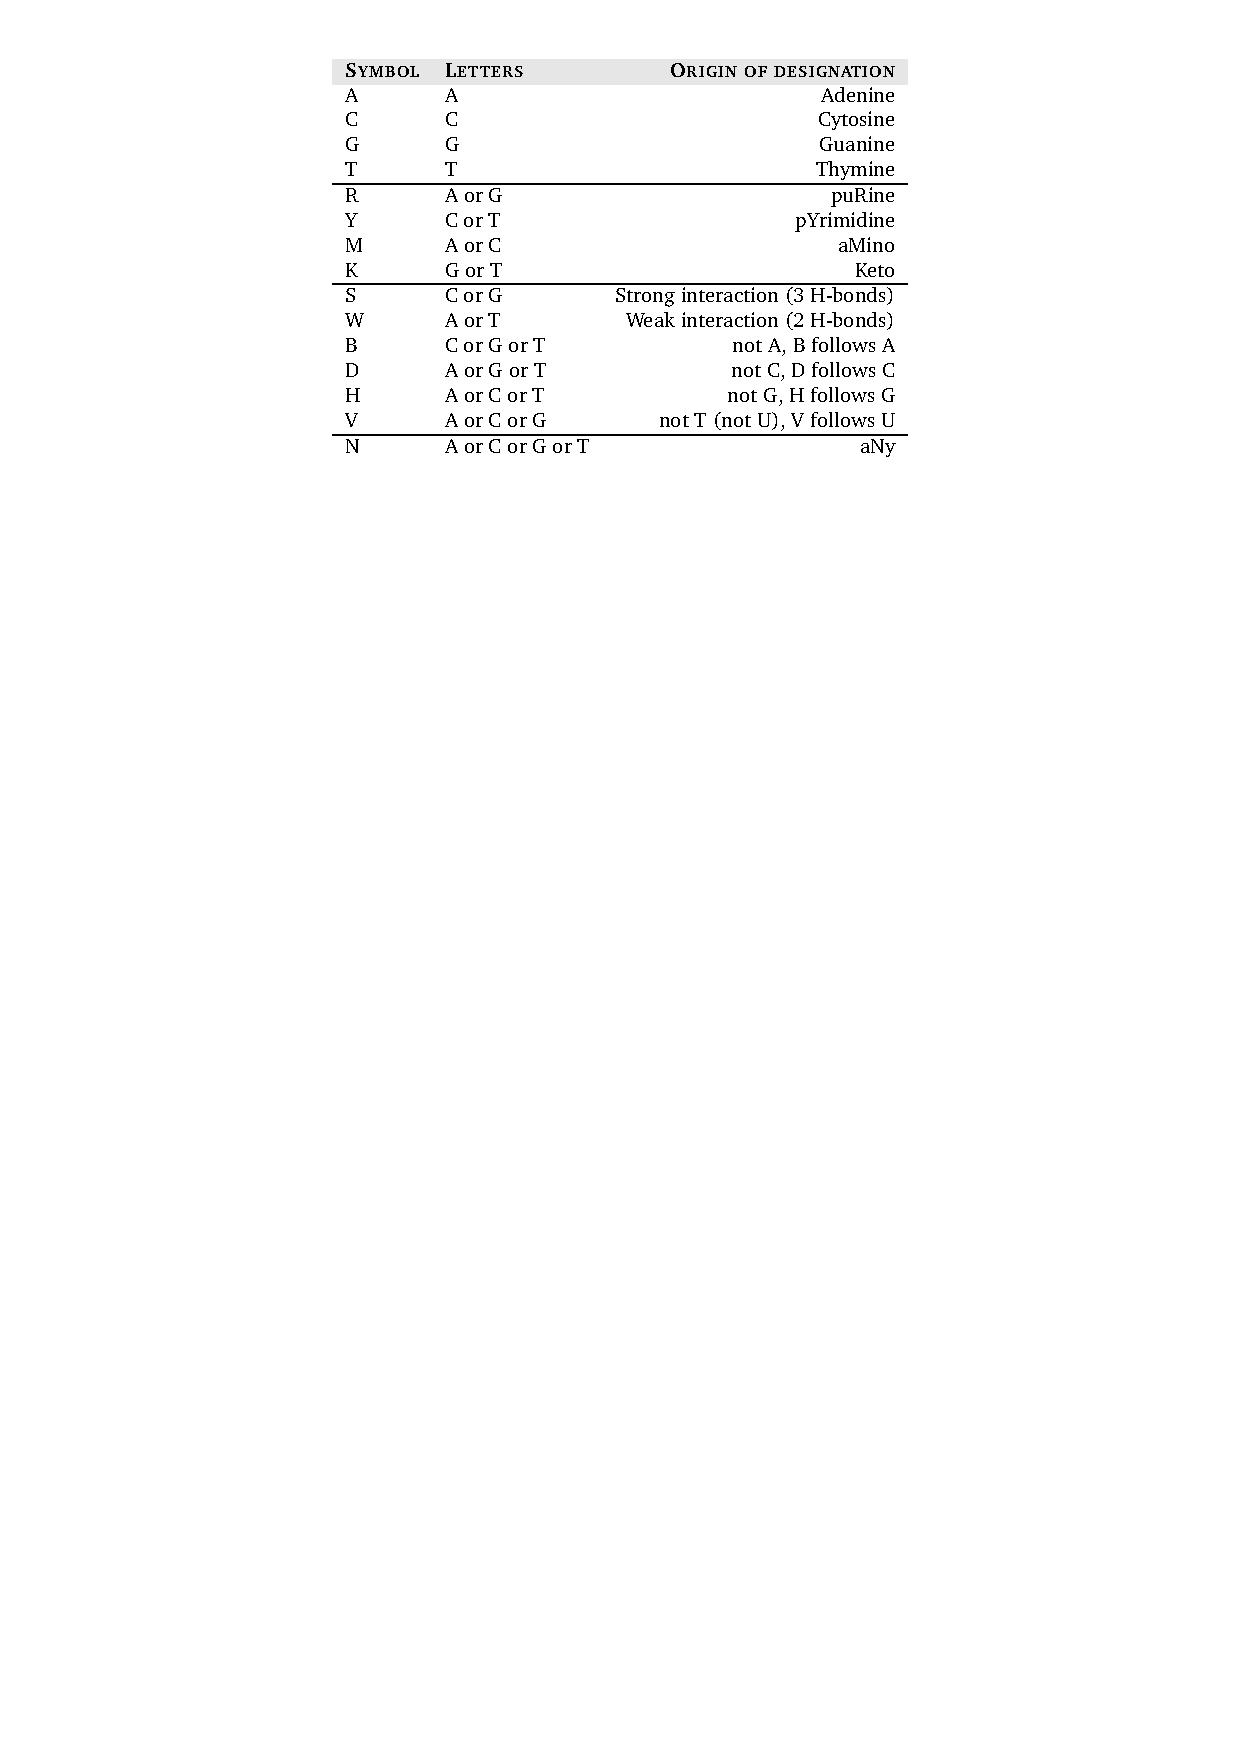
\includegraphics[bb=155 621 498 815,clip]{tables/code1}
\end{minipage}
\mycaption{tab:code1}% label
          {The IUPAC extended genetic alphabet}% lof
          {The IUPAC extended genetic alphabet.}% caption header
          {}
\end{center}
\end{table}


\subsubsectionblue{The number of alignments}

The number of possible alignments between two sequences of $n$ symbols can be computed with the 
following function \citep{waterman:1984a,waterman:1995a}:
\index{alignment!nalns@number of}

\begin{center}
\fcolorbox{white}{verylightgreen}{
\begin{minipage}[][][c]{0.95\linewidth}
\begin{equation}
g(n) \sim \frac{2^{2n}}{4\sqrt{n\pi}}.
\end{equation}
\end{minipage}}
\end{center}

For two sequences of $1,000$ nucleotides, $g(n) > 10{^{600}}$. As direct examination of all these 
alignments is in practice impossible, computational approaches are therefore essential to calculate 
the optimal alignment without exploring all of the combinations.

%%%%
% Table 2: AA alphabet
%%%%
\begin{table}[t!]
\begin{center}
\begin{minipage}{0.4\linewidth}\setlength{\parindent}{0pt}
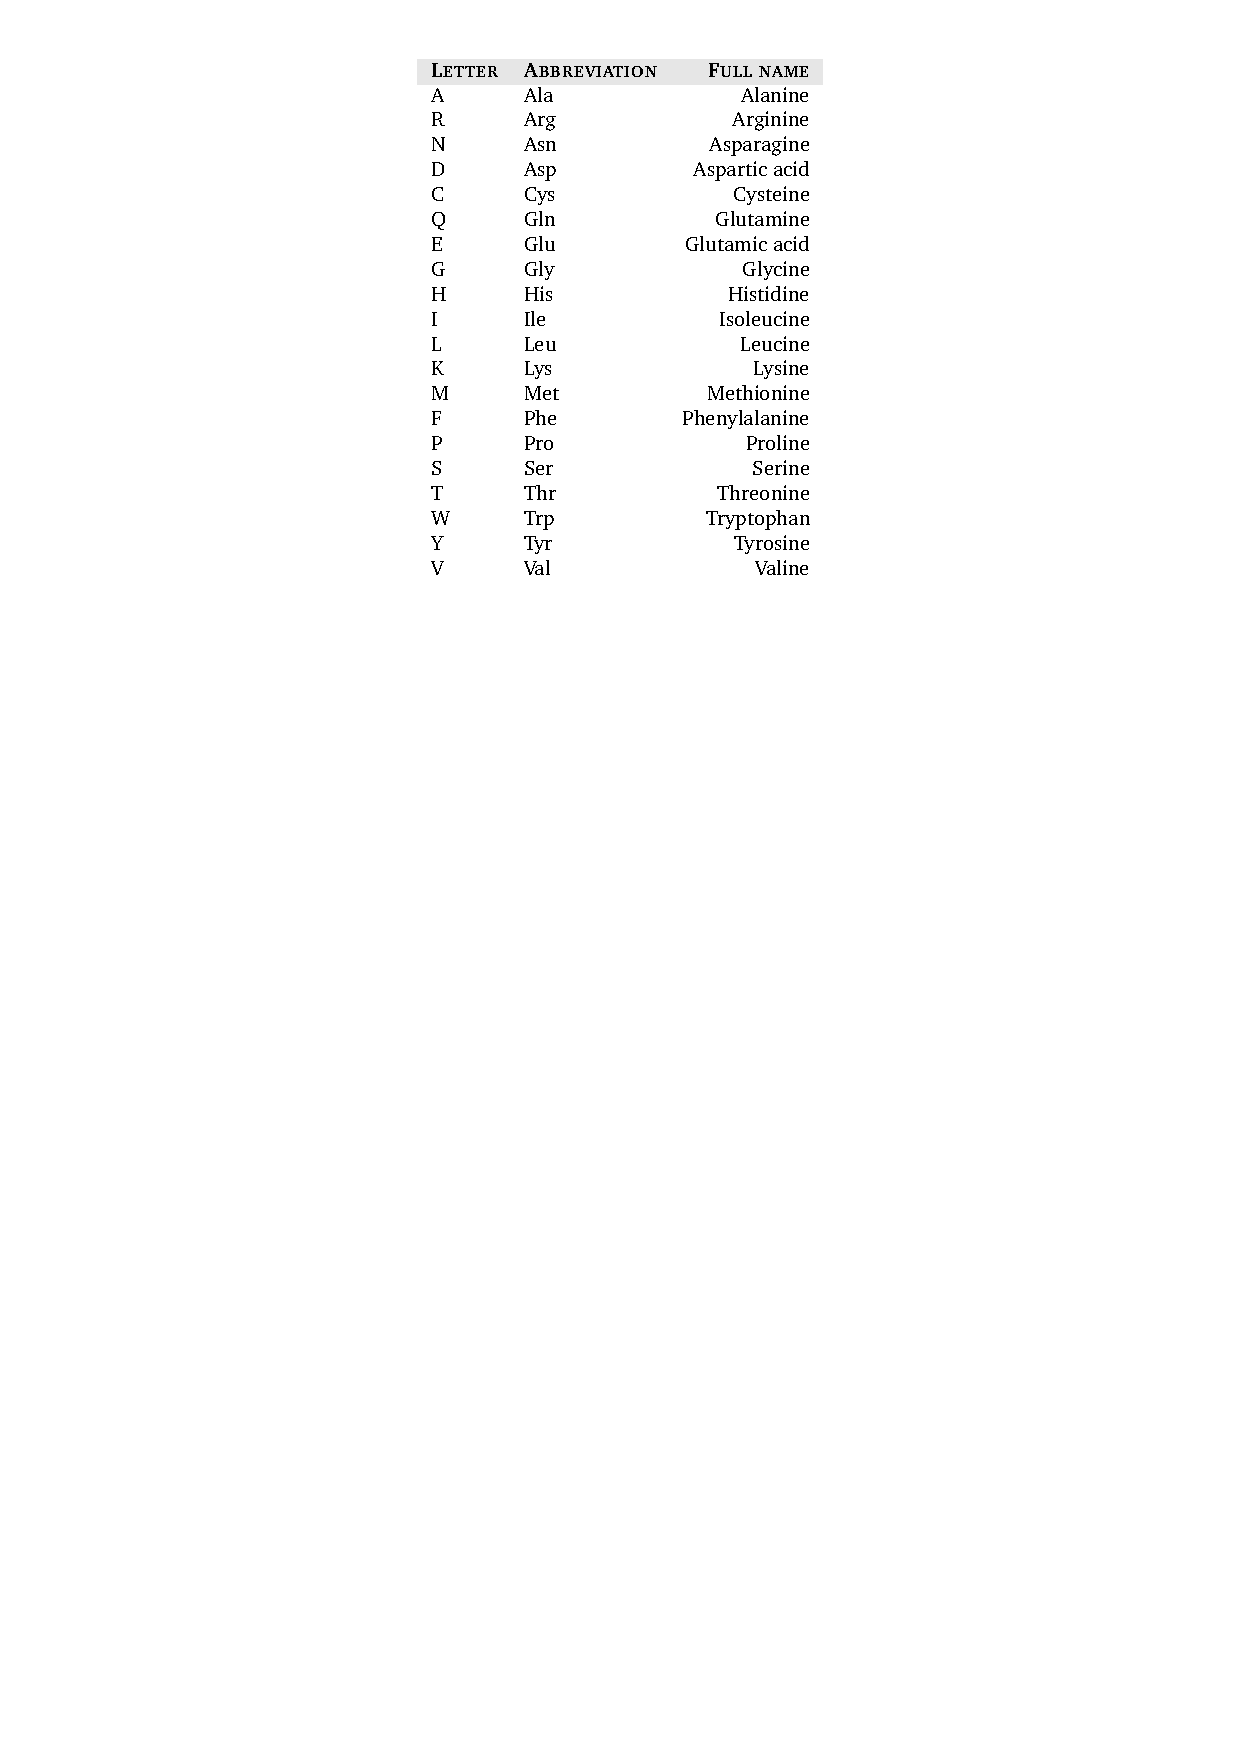
\includegraphics[bb=200 564 397 817,clip]{tables/code2}
\end{minipage}
\mycaption{tab:code2}% label
          {The amino acid alphabet}% lof
          {The amino acid alphabet.}% caption header
          {}
\end{center}
\end{table}

\subsectionblue{Classes of sequence alignments}\label{subsec:classes}
\index{alignment!class@classes}
According to the type of comparison that must be performed between sequences, sequence alignments can 
classified as \citep{mount:2001a}:

\begin{mitemize}
\item
Global alignments: \index{alignment!glob@global}
the entire sequence length must be aligned to include the maximum number of matches. 
Sequences that are quite similar and approximately have the same length are good candidates for global alignment.
\begin{center}
\fcolorbox{white}{verylightgreen}{
\begin{minipage}[][][c]{0.95\linewidth}
\begin{center}
\begin{tabular}{ccccccccccccccccccc}
L & G & P & S & S & K & Q & T & G & K & G & S & -- & S & R & I & W & D & N\\ 
| & & & & & | & & & | & | & | & & & & | & & & | & \\
L & N & -- & I & T & K & S & A & G & K & G & A & I & M & R & L & G & D & A\\
\end{tabular}
\end{center}
\end{minipage}}
\end{center}

\item
Local alignments: \index{alignment!loc@local}
only the stretches of the sequences with the highest density of matches are aligned.
Sequences that differ in length or that only share certain regions are suitable candidates
for local alignment.

\begin{center}
\fcolorbox{white}{verylightgreen}{
\begin{minipage}[][][c]{0.95\linewidth}
\begin{center}
\begin{tabular}{ccccccccccccccccccc}
-- & -- & -- & -- & -- & -- & -- & T & G & K & G & -- & -- & -- & -- & -- & -- & -- & --\\ 
 & & & & & & & & | & | & | & & & & & & & & \\
-- & -- & -- & -- & -- & -- & -- & A & G & K & G & -- & -- & -- & -- & -- & -- & -- & --\\
\end{tabular}
\end{center}
\end{minipage}}
\end{center}
\end{mitemize}

When the number of sequences is two, such alignments receive the name of pairwise alignments
\index{alignment!paraln@pairwise}
as the examples above. If the number of input sequences is higher, they are called multiple sequence
alignments:\index{alignment!mul@multiple}

\begin{mitemize}
\item
Global multiple alignments: the whole set of sequences is aligned at their entire length.
Simply known as multiple alignments, they are the starting point for evolutionary modeling. Each 
column of the alignment is examined and significant changes observed in this position collaborate 
in the construction of a phylogenetic tree. 
\begin{center}
\fcolorbox{white}{verylightgreen}{
\begin{minipage}[][][c]{0.95\linewidth}
\begin{center}
\begin{tabular}{ccccccccccccccccccc}
L & G & P & S & S & K & Q & T & G & K & G & S & -- & S & R & I & W & D & N\\ 
| & & & & & & & & | & | &  & & & &  & & & | & \\
L & N & -- & I & T & K & S & A & G & K & G & A & I & M & R & L & G & D & A\\
| &  & & & & & & & | & | &  & & & & & & & | & \\
L & N & -- & K & Q & Q & S & A & G & K & C & A & I & M & -- & L & G & D & A\\
\end{tabular}
\end{center}
\end{minipage}}
\end{center}

\item
Local multiple alignments: they are equivalent to searching a pattern conserved in a set of sequences.
Rather than be defined as a form of alignment, it is conceptually considered a pattern discovery 
problem.

\begin{center}
\fcolorbox{white}{verylightgreen}{
\begin{minipage}[][][c]{0.95\linewidth}
\begin{center}
\begin{tabular}{ccccccccccccccccccc}
-- & -- & -- & -- & -- & -- & -- & T & G & K & G & -- & -- & -- & -- & -- & -- & -- & --\\ 
-- & -- & -- & -- & -- & -- & -- & A & G & K & G & -- & -- & -- & -- & -- & -- & -- & --\\
-- & -- & -- & -- & -- & -- & -- & A & G & K & C & -- & -- & -- & -- & -- & -- & -- & --\\
\end{tabular}
\end{center}
\end{minipage}}
\end{center}
\end{mitemize}


\sectionorange{An anthology of algorithms for global alignments}\label{sec:global}

This section aims to be a catalogue of different approaches to solve the global pairwise alignment which
was the first problem introduced in the field of sequence comparisons. Naturally, the extension to the
multiple alignment of sequences has been also treated although optimal solutions were discarded because of 
their expensive time and space costs. Different heuristics to cope with multiple alignment are explained 
in detail in Section \ref{sec:msa}.

\subsectionblue{The Needleman and Wunsch algorithm (1970)}\label{nw}

\index{algorithms!nw@Needleman and Wunsch} \index{alignment!nw@Needleman and Wunsch}
For the authors, the similarity or maximum match value between two proteins depends on the largest number
of amino acids from the first protein that can be matched with those of the second one allowing possible 
interruptions in either sequence. 

Each pair of amino acids from each sequence is the smallest unit of significance. All possible pair 
combinations are represented in a two-dimensional matrix $M$. The pathways through the cells of the 
matrix are representations of every possible comparison of the two sequences. If a given value is 
assigned to each identity and mismatch, the maximum match between two sequences $A$ and $B$ is then 
the largest number that would result from the sum of the cell values of every pathway.

The original \citeauthor{needleman:1970a} algorithm is actually a description of a method to 
systematically count the number of identities (denoted as 1's in the simplest formulation) between both 
sequences. No complexity analysis was provided although a careful analysis determines the cost of the
process is cubic (see next section). In addition, the authors implicitly suggested the extension of 
the method to allow multiple comparison of several proteins or the inclusion of a gap penalty factor as 
a function depending on the length of the gap.

The assessment of the significance of a given match value was also proposed: first, two sets of random 
sequences with the same composition of the original proteins are constructed; second, the maximum-match 
between pairs of these sequences is determined several times and is compared to the value obtained between 
real proteins; third, the match between one of the real proteins and several of the random sequences 
is also computed and evaluated. In all of the cases, the difference between the real match and the 
artificial ones should be statistically significant. Otherwise, the match between both proteins would be 
explained in part only by a similar composition.

%%%%
% Figure 2: N-W Matrix (figure 1 paper)
%%%%
\begin{figure}[t!]
\begin{center}
\setlength{\fboxsep}{0pt}
%\fbox{
\incgraph{width=0.4\linewidth}{ps/nw}%}
\mycaption{fig:nw}% label
          {The maximum-match operation for necessary pathways}% lof
          {The maximum-match operation for necessary pathways.}% caption header
          {The cell $(R,R,1)$ corresponds to the current $M(i,j)$. Adapted from \citet{needleman:1970a}.}
\end{center}
\end{figure}

\subsubsectionblue{Formulation and cost}

The objective of the algorithm is to compute the pathway in the matrix $M$ that according to a certain
scoring schema is assigned the maximum value. The procedure to efficiently compute this value consists 
of two stages (see Figure \ref{fig:nw}):
\begin{menumerate}
\item
Each cell of the matrix $M(i,j)$ is assigned the corresponding value whether there is a match or a 
mismatch in this position (e.g. $1$ for identities, void or $0$ for mismatches).
\item
Beginning at the terminals of the sequences and proceeding toward the origins in the matrix, the value 
of the maximum-match starting at each cell $M(i,j)$ can be obtained by adding to its value, the maximum
value from among all the cells which lie on a pathway to it. The pathways are negatively weighted with the 
value $g$ according to the number of gaps they contain. 
\end{menumerate}

\begin{center}
\fcolorbox{white}{verylightgreen}{
\begin{minipage}[][][c]{0.95\linewidth}
\begin{equation}
M(i,j) = M(i,j) +
max
\left\{
\begin{array}{lr}
M(i+1,j+1) &\\
M(i',j+1) + g \times (i' -i + 1),& i+2 \leq i' \leq |A| \\
M(i+1,j') + g \times (j' -j + 1),& j+2 \leq j' \leq |B|. \\
\end{array}\right.
\end{equation}
\end{minipage}}
\end{center}

If $|A| = |B| = n$, then the cost of visiting each cell of the matrix is $O(n^2)$. Additionally, for 
each cell the best pathway among all of the possible ones in the previous row, in the previous column 
and in the diagonal is searched. The cost of accessing the values of the pathways in a given column or 
row is $O(n)$, while accessing the diagonal is constant $O(1)$. Therefore, the final cost of the 
\citeauthor{needleman:1970a} algorithm is $O(n^3)$.

\subsubsectionblue{Implementation}

The implementation of the algorithm is shown in Figure \ref{fig:nwalg}. The matrix is processed
following a systematic order. Both processing steps described above are integrated in a single 
one. For each pair of amino acids from both sequences represented by a cell $M(i,j)$ in the matrix , the 
optimal pathway starting there is constructed selecting the best pathway in the diagonal, and in the 
$i+1$ row and the $j+1$ column (here weighting according to the number of gaps) that have been 
previously computed.

The matrix $P$ is used to record the cell from which the maximum pathway was selected. The retrievement 
of the solution, not shown here, consists on (1) searching the maximum value (cell $x,y$) both in the first 
row and in the first column and (2) using recursively the coordinates in $P(x,y)$, to construct the 
arrangement of both sequences until a cell at the last column or row is reached.


\subsectionblue{The Sellers algorithm (1974)}\label{sellers}

\index{algorithms!sellers@Sellers} \index{alignment!selal@Sellers}
In the 1970s, most techniques used in taxonomic tree construction depended on the introduction
of a measure of distance between sequences \citep{fitch:1967a}. The work on distances or metrics on
protein sequences was essentially based on discovering what genetic mutations were required to change
one sequence into another.

\clearpage
A metric space is a function $\rho: S \times S \rightarrow \mathcal{Z^+}$ on a generic set $S$, with 
the following properties:

\begin{center}
\fcolorbox{white}{verylightgreen}{
\begin{minipage}[][][c]{0.95\linewidth}
\begin{center}
\begin{tabular}{ll}
\emph{Non-negative} & $\forall a,b \in S: \rho(a,b) \geq 0$\\
\emph{Identity} & $\forall a,b \in S: \rho(a,b) = 0 \Leftrightarrow a = b$\\
\emph{Reflexivity} & $\forall a,b \in S: \rho(a,b) = \rho(b,a)$\\
\emph{Transitivity} & $\forall a,b,c \in S: \rho(a,b) \leq \rho(a,c) + \rho(c,b)$.\\
\end{tabular}
\end{center}
\end{minipage}}
\end{center}

\citet{sellers:1974a} described the construction of an evolutionary tree, which assumes that evolutionary
distance is a metric. The minimum distance $D(A,B)$ between two sequences $A$ and $B$ is defined as the 
smallest possible weighted sum of insertions, deletions, and substitutions which transforms one sequence
into the other.

\citeauthor{sellers:1974a} showed that if a scoring function $d(a,b)$\footnote{Also known as a weighting 
scheme.} forms a metric space over the underlying alphabet of symbols then the minimum distance function 
$D(A,B)$ forms a metric space over the set of finite sequences constructed with such an alphabet. In 
addition, he proportioned the dynamic programming recurrence to efficiently compute the minimum distance $D$
between two sequences using several scoring functions. In fact, many comparison algorithms that use 
distance functions with a given weighting scheme provide an optimal alignment only if such a scheme is a 
metric \citep{tyler:1991a}.


%%%%
% Figure 3: N-W algorithm
%%%%
\begin{figure}[t!]
\begin{center}
\scalebox{1}{
\fcolorbox{white}{verylightgreen}{
\begin{minipage}[][][c]{0.95\linewidth}
\begin{algorithmic}[5]
\REQUIRE $A,B$: sequences; id,mis,gap $\in \mathcal{Z}$
\STATE
\STATE \COMMENT{Begin the series of sums from last row and column}
\FOR{$i=|A|$ to $1$}
\FOR{$j=|B|$ to $1$}
\STATE \COMMENT{Setting the identity or mismatch value for the cell}
\IF{$a_i = b_j$}
\STATE $M(i,j) \leftarrow$ id;
\ELSE
\STATE $M(i,j) \leftarrow$ mis;
\ENDIF
\IF{$i \neq |A|$ and $j \neq |B|$}
\STATE \COMMENT{Search the maximum-match pathway beginning here}
\STATE \COMMENT{A. The maximum from diagonal}
\STATE max $\leftarrow M(i+1,j+1)$;
\STATE $P(i,j) \leftarrow (i+1,j+1)$;
\STATE \COMMENT{B. The maximum value from previous column}
\STATE ngaps $\leftarrow 1$;
\FOR{$i'= i + 2$ to $|A|$}
\STATE value $\leftarrow M(i',j+1) + \mbox{gap * ngaps}$; 
\IF{value $> \mbox{max}$}
\STATE max $\leftarrow$ value;
\STATE $P(i,j) \leftarrow (i',j+1)$;
\ENDIF
\STATE ngaps $\leftarrow$ ngaps + 1;
\ENDFOR
\STATE \COMMENT{C. The maximum value from previous row}
\STATE ngaps $\leftarrow 1$;
\FOR{$j'= j + 2$ to $|B|$}
\STATE value $\leftarrow M(i+1,j') + \mbox{gap * ngaps}$;
\IF{value $> \mbox{max}$}
\STATE max $\leftarrow $ value;
\STATE $P(i,j) \leftarrow (i+1,j')$;
\ENDIF
\STATE ngaps $\leftarrow$ ngaps + 1;
\ENDFOR
\STATE \COMMENT{The maximum-match pathway is formed}
\STATE $M(i,j) \leftarrow M(i,j) + \mbox{max}$;
\ENDIF
\ENDFOR
\ENDFOR
\end{algorithmic}
\end{minipage}}}
\mycaption{fig:nwalg}% label
          {The \citeauthor{needleman:1970a} algorithm}% lof
          {The \citeauthor{needleman:1970a} algorithm.}% caption header
          {}
\end{center}
\end{figure}


\subsubsectionblue{Formulation and cost}

\citeauthor{sellers:1974a} generalized the algorithm to allow for various weighting schemes. Let $a$ and $b$ be two
symbols. The simplest scheme $d$ to score this match is defined as:

\begin{center}
\fcolorbox{white}{verylightgreen}{
\begin{minipage}[][][c]{0.95\linewidth}
\begin{equation}
d(a,b) = 
\left\{
\begin{array}{lr}
0 & \mbox{if}~~a = b\\
1 & \mbox{if}~~a \neq b.\\
\end{array}\right.
\end{equation}
\end{minipage}}
\end{center}

Using this scoring function $d$, the following recurrence calculates the optimal distance between two
sequences $A = (a_1, a_2, \ldots a_m)$ and $B = (b_1, b_2, \ldots b_n)$, and provides the initial values as well:

\begin{center}
\fcolorbox{white}{verylightgreen}{
\begin{minipage}[][][c]{0.95\linewidth}
\begin{equation}
\begin{array}{ll}
D(i,j) = &
min \left\{
\begin{array}{ll}
D(i-1,j-1) + d(a_i,b_j) & \mbox{\emph{Match}}\\
D(i-1,j) + d(a_i,-) & \mbox{\emph{Gap in $B$}}\\
D(i,j-1) + d(-,b_j) & \mbox{\emph{Gap in $A$}}\\
\end{array}\right. ,\\[0.75cm]

D(i,0) = & \sum_{k=0}^{i}{d(a_k,-)},\\
D(0,j) = & \sum_{k=0}^{j}{d(-,b_k)}.
\end{array}
\label{eq:sellers}
\end{equation}
\end{minipage}}
\end{center}

To avoid the exponential number of combinations to construct an alignment between two sequences, this
dynamic programming recurrence decompose the problem in smaller alignments of prefixes of the original
sequences. Thus, starting from the one-letter prefixes , the minimum distance of the alignment 
ending at the prefixes $A_{1,i}$ and $B_{1,j}$ can be calculated from the three different forms of finishing
such an alignment:

\begin{center}
\fcolorbox{white}{verylightgreen}{
\begin{minipage}[][][c]{0.95\linewidth}
\begin{center}
%\scalebox{0.7}{
%\begin{minipage}[][][c]{1.25\linewidth}
\begin{tabular}{ccc}
\fbox{\begin{tabular}{lllll}
$\bullet$ & $\bullet$ & $\bullet$ & $\bullet$ & $a_i$\\
$\bullet$ & $\bullet$ & $\bullet$ & $\bullet$ & $b_j$\\
\end{tabular}}
&
\fbox{\begin{tabular}{lllll}
$\bullet$ & $\bullet$ & $\bullet$ & $\bullet$ & $a_i$\\
$\bullet$ & $\bullet$ & $\bullet$ & $\bullet$ & --\\
\end{tabular}}
&
\fbox{\begin{tabular}{lllll}
$\bullet$ & $\bullet$ & $\bullet$ & $\bullet$ & --\\
$\bullet$ & $\bullet$ & $\bullet$ & $\bullet$ & $b_j$\\
\end{tabular}}\\
Match & Ins in $A$, Del in $B$ & Del in $A$, Ins in $B$.\\
\end{tabular}
%\end{minipage}}
\end{center}
\end{minipage}}
\end{center}

%%%%
% Figure 4: DProgramming Matrix
%%%%
\begin{figure}[t!]
\begin{center}
\setlength{\fboxsep}{0pt}
%\fbox{
\incgraph{width=0.6\linewidth}{ps/dp}%}
\mycaption{fig:dp}% label
          {The dynamic programming matrix}% lof
          {The dynamic programming matrix.}% caption header
          {In yellow, the part of the alignment matrix that has been computed. In blue, the part that must be still calculated. The cell $D(i,j)$ is the match currently in process.}
\end{center}
\end{figure}

If both sequences have the same length $n$, the cost of the \citeauthor{sellers:1974a} algorithm is 
$O(n^2)$ which is the time to visit all of the cells of the dynamic programming matrix (see Figure 
\ref{fig:dp}). For each cell, only three neighbours are consulted: in the diagonal, in the horizontal
and in the vertical.

The procedure to trace-back the distance matrix, reconstructing the alignment was adapted from
\citeauthor{needleman:1970a} by \citeauthor{sellers:1974a}. A second matrix of pointers is needed for 
recording from which direction was taken the value to update a given cell matrix.

\subsubsectionblue{Implementation}

The \citeauthor{sellers:1974a} algorithm requires to fit the \citeauthor{needleman:1970a} $m \times n$
matrix in an artificial 0-column and 0-row to increase the initial distance when starting the alignment 
with gaps\footnote{There is an easy modification of the algorithm to permit not to punish this kind of 
gaps.}. 

Then, the algorithm starts at $D(1,1)$ and the matrix is filled by rows (from top to bottom) and within a 
row by columns (from left to right). Thus, when a cell $D(i,j)$ is reached, its neigbours $D(i-1,j-1)$, 
$D(i-1,j)$ and $D(i,j-1)$ have been already calculated.

%%%%
% Figure 5: Sellers algorithm
%%%%
\begin{figure}[t!]
\begin{center}
\scalebox{1}{
\fcolorbox{white}{verylightgreen}{
\begin{minipage}[][][c]{0.95\linewidth}
\begin{algorithmic}[5]
\REQUIRE $A,B$: sequences;  $d$: metric on $\Sigma$
\STATE
\STATE \COMMENT{Initialize the 0-column and the 0-row}
\FOR{$i=0$ to $|A|$}
\STATE $D(i,0) \leftarrow i \times d(a_i,-)$;
\ENDFOR
\FOR{$j=1$ to $|B|$}
\STATE $D(0,j) \leftarrow j \times d(b_j,-)$;
\ENDFOR
\STATE \COMMENT{Filling the matrix}
\FOR{$i=1$ to $|A|$}
\FOR{$j=1$ to $|B|$}
\STATE \COMMENT{A. Match}
\STATE min $\leftarrow D(i-1,j-1) + d(a_i,b_j)$;
\STATE $P(i,j) \leftarrow (i-1,j-1)$;
\STATE \COMMENT{B. Gap in sequence $B$}
\STATE value $\leftarrow D(i-1,j) + d(a_i,-)$;
\IF{value $<$ min}
\STATE min $\leftarrow$ value;
\STATE $P(i,j) \leftarrow (i-1,j)$;
\ENDIF
\STATE \COMMENT{C. Gap in sequence $A$}
\STATE value $\leftarrow D(i,j-1) + d(-,b_j)$;
\IF{value $<$ min}
\STATE min $\leftarrow$ value;
\STATE $P(i,j) \leftarrow (i,j-1)$;
\ENDIF
\STATE $D(i,j) \leftarrow$ min;
\ENDFOR
\ENDFOR
\end{algorithmic}
\end{minipage}}}
\mycaption{fig:sellersalg}% label
          {The \citeauthor{sellers:1974a} algorithm}% lof
          {The \citeauthor{sellers:1974a} algorithm.}% caption header
          {}
\end{center}
\end{figure}

Contrarily to the \citeauthor{needleman:1970a} algorithm (in which the maximum match was searched in the 
last column and the last row), the minimum distance between both sequences will be saved at the end into 
the cell $D(m,n)$ because of the different initialization.

As in the case of the \citeauthor{needleman:1970a}, there is an auxiliary matrix $P$ that saves the 
source of each calculation in a given cell to recursively reconstruct the alignment with such a distance.

\subsectionblue{A linear space algorithm: Hirschberg (1975)}\label{linearspace}

\index{algorithms!hirs@Hirschberg} \index{alignment!hirsal@Hirschberg}
In some occasions when aligning two sequences, the limiting factor is not the time but the space (memory).
Any algorithm that solves the alignment of two sequences can not decrease the quadratic time cost unless
any assumption is made over the length of the inputs. However, the quadratic cost in terms of space can 
be reduced to a linear cost.

\citet{hirschberg:1975a} designed a divide and conquer algorithm to solve the LCS problem in linear space
without increasing the asymptotic time cost. Later, \citet{myers:1988a} demonstrated how this technique
could optimally deal with general sequence alignment problems.

The key point of the algorithm is based on the fact that in the alignment between the sequences $A$ and
$B$, any element of $A$ will be aligned either to a gap or another element in $B$. Thus, the problem
of aligning both sequences can be expressed in terms of making this decision for a current element $a_i$,
assuming the optimal alignments between the subsequences from $A$ and $B$ around this element are already 
computed.

Another important fact is the ability to compute the distance between two sequences in linear space.
If the dynamic programming matrix is filled in from top to bottom (row by row), and fixing a row, from
left to right (column by column), then the values in a row $i$ depend only on the values stored at the 
previous row $i-1$ and on the values in the same row $i$. The other previous rows are therefore not necessary
to obtain the final value $D(m,n)$ \citep{myers:1991a,meidanis:1997a}.

Furthermore, instead of using two arrays to represent the rows $i$ and $i+1$, the computation can be 
performed in a single array $D$ (see Figure \ref{fig:twoarray} (A)), overwriting the old values on the left 
of the current column $j$. The equivalence between each cell $D(i,j)$ in the original dynamic programming matrix 
and the content of this unidimensional array $D$ when the row $i$ is being processed is:

\begin{center}
\fcolorbox{white}{verylightgreen}{
\begin{minipage}[][][c]{0.95\linewidth}
\begin{equation}
\begin{array}{l}
D(k) \approx D(i,k) ~~\mbox{when}~~ k < j ~~\mbox{(current row, $i$)}\\
D(k) \approx D(i-1,k) ~~\mbox{when}~~ k \geq j ~~\mbox{(previous row, $i-1$)}.\\
\end{array}
\end{equation}
\end{minipage}}
\end{center}

%%%%
% Figure 6: Using an array to compute D(i,j)
%%%%
\begin{figure}[t!]
\begin{center}
\setlength{\fboxsep}{0pt}
\begin{tabular}{ccc}
%\hline
%\hline
\incgraph{width=4cm,height=4cm}{ps/hir1} &
\incgraph{width=4cm,height=4cm}{ps/hir2} &
\incgraph{width=4cm,height=4cm}{ps/hir3}\\
%\hline
A & B & C
\end{tabular}
\mycaption{fig:twoarray}% label
          {The \citeauthor{hirschberg:1975a} linear space approach}% lof
          {The \citeauthor{hirschberg:1975a} linear space approach.}% caption header
          {(A) Using a single array to compute $D(i,j)$. (B) The divide and conquer strategy applied over the dynamic programming approach. (C) The backward propagation of values.}
\end{center}
\end{figure}

\subsubsectionblue{Formulation and cost}

In the optimal alignment between two sequences $A$ and $B$, a given element $a_i$ from $A$ will be either
matched to another element $b_j$ from $B$ or aligned to a gap between a certain $b_j$ and $b_{j+1}$. Then,
this optimal alignment can be decomposed in three parts:

\begin{menumerate}
\item
The optimal alignment between the elements from both sequences on the left (prefixes).
\item
The match between $a_i$ with a certain $b_j$ or a gap.
\item
The optimal alignment between the elements from both sequences on the right (suffixes).
\end{menumerate}

For a given $i$, the optimal point $j$ can be unveiled with the application of the algorithm to compute 
only the distance between two sequences in linear space time. Such a solution provides the point in 
which the optimal alignment path will cross the $i$-row in the the dynamic programming matrix. As it is 
shown in Figure \ref{fig:twoarray} (B), once the points $i$ and $j$ are established, the general 
problem is divided into two subproblems and recursively the same procedure is applied until reaching the 
base case (empty sequences).

The algorithm that computes only the distance between two sequences in linear space is in fact a method
to provide the minimum distance between the first sequence and any of the prefixes of the second sequence. 
As the right parts are also aligned in the main procedure, a modification of such an algorithm is 
necessary to obtain the minimum distance between the first sequence and any of the suffixes of the second 
one.

In fact, the dynamic programming scheme is not restricted to construct the final alignment from 
alignments between prefixes of the input sequences. The same recurrence is appropriate for building it
from alignments between suffixes of them. The procedure now begins in the position $D(|A|,|B|)$, and
propagates the values from bottom to top, and from right to left (see Figure \ref{fig:twoarray} (C)). 
The Equation \ref{eq:sellers} must be slightly modified to accommodate this backward propagation:

\begin{center}
\fcolorbox{white}{verylightgreen}{
\begin{minipage}[][][c]{0.95\linewidth}
\begin{equation}
\begin{array}{ll}
D(i,j) = &
min \left\{
\begin{array}{ll}
D(i+1,j+1) + d(a_i,b_j) & \mbox{\emph{Match}}\\
D(i+1,j) + d(a_i,-) & \mbox{\emph{Gap in $B$}}\\
D(i,j+1) + d(-,b_j) & \mbox{\emph{Gap in $A$}}\\
\end{array}\right. ,\\[0.75cm]

D(i,|B|+1) = & \sum_{k=0}^{i}{d(a_k,-)},\\
D(|A|+1,j) = & \sum_{k=0}^{j}{d(-,b_k)}.\\
\end{array}
\end{equation}
\end{minipage}}
\end{center}

The cost of obtaining just the value $D(i,j)$ following the forward or the backward manner is again 
quadratic in terms of time. However, the cost in terms of space of this function is linear as 
only a single array is used in both cases.

To compute the cost of a recursive divide and conquer function, a different cost scheme must be applied.
Let us consider $n$ the length of both input sequences that are aligned. At the beginning, the routine
performs some computations and then, there is an approximate $\frac{n}{2}$ reduction in the size of the 
input data for the subsequent two recursive calls. The cost $T(n)$ of computing such a recursive function 
can be expressed in terms of its children as:

\begin{center}
\fcolorbox{white}{verylightgreen}{
\begin{minipage}[][][c]{0.95\linewidth}
\begin{equation}
\begin{array}{l}
T(n) = 
\left\{
\begin{array}{lll}
g(n) & 0 \leq n < c & \mbox{\emph{Base case}}\\
a T(\frac{n}{c}) + b n^k & n \geq c & \mbox{\emph{Recursive case}}\\
\end{array}\right.,
\end{array}
\end{equation}
\end{minipage}}
\end{center}

where $a$ is the number of recursive calls, $c$ is the size of the fragmentation and $b n^k$ is the
cost of the non-recurrent operations performed on each call. From the relationship between $a$ and $c^k$, 
the corresponding cost function is inferred following the Master Theorem of recurrent equations (see 
\citet{cormen:2001a}, Sections 4.3 and 4.4). In the \citeauthor{hirschberg:1975a} recurrence is easy to 
notice $g(n) \in O(n)$, $a = 2$, $b = 2$, $c = 2$ and $k = 2$. Therefore as $a<c^k$ or $2<2^2$, according to 
the Master Theorem $T(n) \in \Theta(n^k)$, that is $T(n) \in \Theta(n^2)$. 

Nevertheless, the spatial cost of the \citeauthor{hirschberg:1975a} algorithm is linear. All of the computations 
on the theoretical dynamic programming matrix are performed over single rows implemented with unidimensional
arrays.


%%%%
% Figure 7: Computing D(m,n) in O(n) space: FWD and RVS
%%%%
\begin{figure}[t!]
\begin{center}
\scalebox{0.7}{
\fcolorbox{white}{verylightgreen}{
\begin{tabular}{c|c}
\begin{minipage}[][][c]{0.6\linewidth}
\textbf{Procedure} ComputeOnlyDistanceForward\\[0ex]
\begin{algorithmic}[5]
\REQUIRE $A,B$: sequences;  $d$: metric on $\Sigma$
\ENSURE $D$: array (|B|+1);
\STATE
\STATE \COMMENT{Simulating the initialization of the 0-row}
\FOR{$j=0$ to $|B|$}
\STATE $D(j) \leftarrow j \times d(-,b_j)$;
\ENDFOR
\FOR{$i=1$ to $|A|$}
\STATE \emph{diag} $\leftarrow D(0)$;
\STATE \COMMENT{Simulating the initialization of the i-row}
\STATE $D(0) \leftarrow i \times d(a_i,-)$;
\FOR{$j=1$ to $|B|$}
\STATE \COMMENT{This cell will be the next diagonal}
\STATE \emph{temp} $\leftarrow D(j)$;
\STATE \COMMENT{A. Match ($\nwarrow$)}
\STATE min $\leftarrow$ \emph{diag} $+ d(a_i,b_j)$;
\STATE \COMMENT{B. Gap in sequence $A$ ($\uparrow$)}
\STATE value $\leftarrow D(j) + d(a_i,-)$;
\IF{value $<$ min}
\STATE min $\leftarrow$ value;
\ENDIF
\STATE \COMMENT{C. Gap in sequence $B$ ($\leftarrow$)}
\STATE value $\leftarrow D(j-1) + d(-,b_j)$;
\IF{value $<$ min}
\STATE min $\leftarrow$ value;
\ENDIF
\STATE $D(j) \leftarrow$ min;
\STATE \COMMENT{Update diagonal}
\STATE \emph{diag} $\leftarrow$ \emph{temp}
\ENDFOR
\ENDFOR
\end{algorithmic}
\end{minipage}
& % second column
\begin{minipage}[][][c]{0.6\linewidth}
\textbf{Procedure} ComputeOnlyDistanceBackward\\[0ex]
\begin{algorithmic}[5]
\REQUIRE $A,B$: sequences;  $d$: metric on $\Sigma$
\ENSURE $D$: array (|B|+1);
\STATE
\STATE \COMMENT{Simulating the initialization of the last row}
\FOR{$j=|B|$ to $1$}
\STATE $D(j) \leftarrow j \times d(-,b_j)$;
\ENDFOR
\FOR{$i=|A|-1$ to $1$}
\STATE \emph{diag} $\leftarrow D(|B|+1)$;
\STATE \COMMENT{Simulating the initialization of the i-row}
\STATE $D(|B|+1) \leftarrow i \times d(a_i,-)$;
\FOR{$j=|B|$ to $1$}
\STATE \COMMENT{This cell will be the next diagonal}
\STATE \emph{temp} $\leftarrow D(j)$;
\STATE \COMMENT{A. Match ($\nwarrow$)}
\STATE min $\leftarrow$ \emph{diag} $+ d(a_i,b_j)$;
\STATE \COMMENT{B. Gap in sequence $A$ ($\downarrow$)}
\STATE value $\leftarrow D(j) + d(a_i,-)$;
\IF{value $<$ min}
\STATE min $\leftarrow$ value;
\ENDIF
\STATE \COMMENT{C. Gap in sequence $B$ ($\rightarrow$)}
\STATE value $\leftarrow D(j+1) + d(-,b_j)$;
\IF{value $<$ min}
\STATE min $\leftarrow$ value;
\ENDIF
\STATE $D(j) \leftarrow$ min;
\STATE \COMMENT{Update diagonal}
\STATE \emph{diag} $\leftarrow$ \emph{temp}
\ENDFOR
\ENDFOR
\end{algorithmic}
\end{minipage}
\end{tabular}}}
\mycaption{fig:cdistance}% label
          {An algorithm to compute $D(i,j)$ in $O(n)$ space cost}% lof
          {An algorithm to compute $D(i,j)$ in $O(n)$ space cost.}% caption header
          {(Left) The computation is done from $D(0,0)$ to $D(|A|,|B|)$. (Right) The 
           computation is done from $D(|A|+1,|B|+1)$ to $D(1,1)$.}
\end{center}
\end{figure}

\subsubsectionblue{Implementation}

\subsubsectionblue{Computing the value $D(i,j)$ in linear space}

To implement the fusion of the previous row and the current one in a single array in a forward manner, 
the temporary variables \emph{diag} and \emph{temp} are necessary to save the values $D(i-1,j-1)$ 
--diagonal-- and $D(i-1,j)$ --gap in $A$--, respectively. At the end of the forward computation,
the array $D$ will contain the same values as the last row of the bidimensional classic dynamic 
programming matrix, that is, the distance between the sequence $A$ and any of the prefixes of the sequence
$B$. In particular, the array position $D(|B|)$ will contain the distance between the sequences $|A|$ 
and $|B|$

The backward computation is symmetrical to the forward processing. The propagation of values starts now
in the position $D(|B|+1)$, moving the values from right to left, and from bottom to top. At the end of the
backward computation, the array $D$ will contain the same values as the last row of the bidimensional 
reverse dynamic programming matrix, that is the distance between the sequence $A$ and any of the suffixes
of the sequence $B$. In particular, the array position $D(1)$ will contain the distance between the 
sequences $|A|$ and $|B|$.

%%%%
% Figure 8: The alignment of two sequences in linear space
%%%%
\begin{figure}[t!]
\begin{center}
\scalebox{0.8}{
\fcolorbox{white}{verylightgreen}{
\begin{minipage}[][][c]{0.95\linewidth}
\textbf{Procedure} Alignment\\[0ex]
\begin{algorithmic}[5]
\REQUIRE $A,B$: sequences;  $d$: metric on $\Sigma$; $i_1,i_2,j_1,j_2,al_1,al_2 in ~\mathcal{Z}$
\ENSURE \emph{alA}: array ($al_1 .. al_2$), \emph{alB}: array ($al_1 .. al_2$);
\STATE
\IF{$A_{i_1,i_2} = \emptyset$}
\STATE \COMMENT{Base case 1}
\FOR{$k=j_1 to j_2$}
\STATE \emph{alA}$(al_1+k) \leftarrow -$;
\STATE \emph{alB}$(al_1+k) \leftarrow B(j_1+k)$;
\ENDFOR
\STATE $al_2 \leftarrow al_1 + k$;
\ELSIF{$B_{j_1,j_2} = \emptyset$}
\STATE \COMMENT{Base case 2}
\FOR{$k=i_1$ to $i_2$}
\STATE $alA(al_1+k) \leftarrow A(i_1+k)$;
\STATE $alA(al_1+k) \leftarrow -$;
\ENDFOR
\STATE $al_2 \leftarrow al_1 + k$;
\ELSE
\STATE \COMMENT{General case}
\STATE \COMMENT{Select the point $i$}
\STATE $i \leftarrow \lfloor \frac{i_1+i_2}{2} \rfloor$
\STATE \COMMENT{Compute the distance to the prefixes/suffixes of $B$}
\STATE \emph{prefDist} $\leftarrow$ ComputeOnlyDistanceForward($A_{i_1,i},B_{j_1,j_2},d$);
\STATE \emph{suffDist} $\leftarrow$ ComputeOnlyDistanceBackward($A_{i+1,i_2},B_{j_1,j_2},d$);
\STATE \COMMENT{The column 0}
\STATE \emph{posmin} $\leftarrow j_1 -1$;
\STATE \emph{typemin} $\leftarrow$ SPACE;
\STATE \emph{vmin} $\leftarrow$ \emph{prefDist}$(j_1-1) + d(a_i,-) +$ \emph{suffDist}$(j_1-1)$;
\STATE \COMMENT{A sweep along the row $i$}
\FOR{$j = j_1$ to $j_2$}
\STATE \COMMENT{Match}
\STATE \emph{value} $\leftarrow$ \emph{prefDist}$(j-1) + d(a_i,b_j) +$ \emph{suffDist}$(j+1)$;
\IF{\emph{value} $<$ \emph{vmin}}
\STATE \emph{vmin} $\leftarrow$ \emph{value};
\STATE \emph{posmin} $\leftarrow$ $j$;
\STATE \emph{typemin} $\leftarrow$ SYMBOL;
\ENDIF
\STATE \COMMENT{Gap}
\STATE \emph{value} $\leftarrow$ \emph{prefDist}$(j) + d(a_i,-) +$ \emph{suffDist}$(j+1)$;
\IF{\emph{value} $<$ \emph{vmin}}
\STATE \emph{vmin} $\leftarrow$ \emph{value};
\STATE \emph{posmin} $\leftarrow$ $j$;
\STATE \emph{typemin} $\leftarrow$ SPACE;
\ENDIF
\ENDFOR
\STATE \COMMENT{Divide and conquer with these values of $i$ and $j$}
\IF{\emph{typemin} $\leftarrow$ SPACE}
\STATE Align($A$,$B$,$d$,$i_1$,$i-1$,$j_1$,\emph{posmin},$al_1$,$al_{tmp}$);
\STATE \emph{alA}$(al_{tmp}) \leftarrow A(i)$;
\STATE \emph{alB}$(al_{tmp}) \leftarrow -$;
\STATE Align($A$,$B$,$d$,$i+1$,$i_2$,\emph{posmin}$+1$,$j_2$,$al_{tmp}$,$al_2$);
\ELSE
\STATE Align($A$,$B$,$d$,$i_1$,$i-1$,$j_1$,\emph{posmin}$-1$,$al_1$,$al_{tmp}$);
\STATE \emph{alA}$(al_{tmp}) \leftarrow -$;
\STATE \emph{alB}$(al_{tmp}) \leftarrow B(\mbox{\emph{posmin}})$;
\STATE Align($A$,$B$,$d$,$i+1$,$i_2$,\emph{posmin}$+1$,$j_2$,$al_{tmp}+1$,$al_2$);
\ENDIF
\ENDIF
\end{algorithmic}
\end{minipage}}}
\mycaption{fig:linearspace}% label
          {The \citeauthor{hirschberg:1975a} linear space algorithm}% lof
          {The \citeauthor{hirschberg:1975a} linear space algorithm.}% caption header
          {}
\end{center}
\end{figure}

\subsubsectionblue{The divide and conquer algorithm}

The \citeauthor{hirschberg:1975a} linear space algorithm is a function \emph{Alignment} that computes the
position of a given symbol $a_i$ from $A$ in the optimal alignment (aligned to a gap or to a certain $b_j$
from $B$) and then splits the general problem into two smaller subproblems (left and right halves of the 
corresponding sequences).

The initial call is \emph{Alignment}$(A,B,d,1,|A|,1,|B|,0,0)$ where $(0,0)$ are the boundaries (al$_1$,al$_2$)
of the optimal alignment that is in construction. Additionally, a pair of arrays \emph{alA, alB} will
save the correspondence between the symbols from both sequences.

As we divide the problem into two minor parts, the base cases are the empty sequences (alignment of the rest
of the symbols in one sequence with gaps in the other one). The general case selects a middle point or symbol 
$a_i$ from $A$. Then, the distance between the prefix $A_{1,i-1}$ to all of the prefixes of the sequence $B$ 
is computed by the routine \emph{ComputeOnlyDistanceForward}. The routine \emph{ComputeOnlyDistanceBackward} 
likewise calculates the same value between the suffix $A_{i+1,|A|}$ and all of the suffixes of the sequence $B$.

Now, a sweep shifting $j$ along the whole row is perform to detect the point $j$ in which the alignment 
constituted by the prefix of $A$ and a given prefix of $B$, the symbol $a_i$ and a gap or a symbol $b_j$,
and the suffix of $A$ and a given suffix of $B$ is optimal. This operation is easily implemented by 
accessing with the proper indexes the arrays \emph{prefDist} and \emph{suffDist} that were filled in by 
the corresponding \emph{ComputeOnlyDistance} functions.

Once the optimal $j$ for the current $a_i$ has been found, a recursive call to discover the part of the
optimal alignment on the left of this symbol is launched. Then, the conquer step assigns the correct 
position to $a_i$ aligned to a gap or a certain $b_j$ in the alignment (arrays \emph{alA,alB}). Finally, a 
second recursive call is performed to place correctly the right part of the optimal alignment.

The variables \emph{posmin,vmin, typemin} save at each moment the minimum distance value in the loop 
along $j$ and the position and the symbol to be aligned to $a_i$. The type of symbol is important to 
correctly split the sequence $B$ at the divide step.

\subsectionblue{The Needleman and Wunsch algorithm revisited by Smith \emph{et al.} (1981)}\label{nwrevisited}
\index{algorithms!nwr@Needleman and Wunsch revisited} \index{alignment!nwr@Needleman and Wunsch revisited}

Although the denomination of \citeauthor{needleman:1970a} algorithm and \citeauthor{sellers:1974a} algorithm have 
survived throughout the years, the standard formulation in terms of distance and similarity methods that is 
widely known today was provided by \citet{smith:1981b}. In their work, they adapted the \citeauthor{needleman:1970a} 
method to a dynamic programming recurrence complementary to that introduced by \citeauthor{sellers:1974a} and 
presented an analysis of equivalence between both measures (see next section).

The similarity measure did not conserve the mathematical properties of the distance metrics. Nonetheless, 
this revisited version of the algorithm became very popular because it was easily extended to cope with 
the local alignment problem (see Section \ref{sec:local}).

%%%%
% Figure 9: NW revisited
%%%%
\begin{figure}[t!]
\begin{center}
\scalebox{1}{
\fcolorbox{white}{verylightgreen}{
\begin{minipage}[][][c]{0.95\linewidth}
\begin{algorithmic}[5]
\REQUIRE $A,B$: sequences;  $s$: substitution matrix
\STATE
\STATE \COMMENT{Initialize the 0-column and the 0-row}
\FOR{$i=0$ to $|A|$}
\STATE $S(i,0) \leftarrow i \times s(a_i,-)$;
\ENDFOR
\FOR{$j=1$ to $|B|$}
\STATE $S(0,j) \leftarrow j \times s(b_j,-)$;
\ENDFOR
\STATE \COMMENT{Filling the matrix}
\FOR{$i=1$ to $|A|$}
\FOR{$j=1$ to $|B|$}
\STATE \COMMENT{A. Match}
\STATE max $\leftarrow S(i-1,j-1) + s(a_i,b_j)$;
\STATE $P(i,j) \leftarrow (i-1,j-1)$;
\STATE \COMMENT{B. Gap in sequence $B$}
\STATE value $\leftarrow S(i-1,j) + s(a_i,-)$;
\IF{value $>$ max}
\STATE max $\leftarrow$ value;
\STATE $P(i,j) \leftarrow (i-1,j)$;
\ENDIF
\STATE \COMMENT{C. Gap in sequence $A$}
\STATE value $\leftarrow S(i,j-1) + s(-,b_j)$;
\IF{value $>$ max}
\STATE max $\leftarrow$ value;
\STATE $P(i,j) \leftarrow (i,j-1)$;
\ENDIF
\STATE $S(i,j) \leftarrow$ max;
\ENDFOR
\ENDFOR
\end{algorithmic}
\end{minipage}}}
\mycaption{fig:nwrevisitedalg}% label
          {The \citeauthor{needleman:1970a} algorithm revisited}% lof
          {The \citeauthor{needleman:1970a} algorithm revisited.}% caption header
          {}
\end{center}
\end{figure}

\subsubsectionblue{Formulation and cost}

If matches are positively rewarded and gaps are punished negatively, the recurrence for computing the maximum 
similarity between two sequences $A$ and $B$ is:

\begin{center}
\fcolorbox{white}{verylightgreen}{
\begin{minipage}[][][c]{0.95\linewidth}
\begin{equation}
\begin{array}{ll}
S(i,j) = &
max \left\{
\begin{array}{ll}
S(i-1,j-1) + s(a_i,b_j) & \mbox{\emph{Match}}\\
S(i-1,j) + s(a_i,-) & \mbox{\emph{Gap in $B$}}\\
S(i,j-1) + s(-,b_j) & \mbox{\emph{Gap in $A$}}\\
\end{array}\right. ,\\[0.75cm]
S(i,0) = & \sum_{k=0}^{i}{s(a_k,-)},\\
S(0,j) = & \sum_{k=0}^{j}{s(-,b_k)}.\\
\end{array}
\label{eq:sim}
\end{equation}
\end{minipage}}
\end{center}

where the function $s(a_i,b_j)$ provides a positive or a negative value for a given match (mismatch) 
according to the aligned elements. If this is an alignment of proteins, the function $s$ can be  
a popular amino acid substitution matrix with an additional penalty for aligning a symbol to 
a gap.

The cost of this revisited \citeauthor{needleman:1970a} algorithm is $O(n^2)$, being correct the same
analysis explained in the \citeauthor{sellers:1974a} approach.

\subsubsectionblue{Implementation}

This implementation is a symmetric translation from the implementation of the \citeauthor{needleman:1970a} 
algorithm. The same procedures to fill the matrix in and to retrieve the optimal alignment are performed.

\subsectionblue{Equivalence between distance and similarity: Smith \emph{et al.} (1981)}\label{simdist}

\index{similarity!wd@similarity and distance}\index{distance!ws@distance and similarity}
From the formulation of the \citeauthor{needleman:1970a} similarity algorithm and 
the \citeauthor{sellers:1974a} distance algorithm a couple of relevant questions quickly arised:
(1) When are both algorithms equivalent? (2) When do they provide the same set of optimal alignments?
\citet{smith:1981a} stated that the two algorithms are defined to be equivalent if given the
scoring scheme for one algorithm, there is a choice of a scoring scheme for the second algorithm such that
the set of alignments achieving the maximum similarity is equal to the set of alignments achieving the
minimum distance.

Given two sequences $A$ and $B$, the optimal alignment $\mathcal{A}$ that maximizes $S(A,B)$ or minimizes 
$D(A,B)$ can be decomposed into two sections: the matched elements ($\lambda_i$) and the elements in one sequence
that are aligned with gaps in the other one ($\Delta_k$):

\begin{center}
\fcolorbox{white}{verylightgreen}{
\begin{minipage}[][][c]{0.95\linewidth}
\begin{equation}
\begin{tabular}{c|c}
$s(a_i,b_j) = \alpha_k$ & $d(a_i,b_j) = \beta_k$\\
$g(k) \geq 0$ & $g'(k) \geq 0$\\[2ex]
\multicolumn{2}{c}{
\begin{tabular}{ll}
$\lambda_i$ & $\rightarrow$ \# of aligned symbols of type $i$\\
$\Delta_k$ & $\rightarrow$ \# of gaps of length $k$\\[2ex]
\end{tabular}}\\
$S(A,B) = max_{\mathcal{A}} \{ \sum_i{\alpha_i \lambda_i} - \sum_k{g(k) \Delta_k}\}$ & 
$D(A,B) = min_{\mathcal{A}} \{ \sum_i{\beta_i \lambda_i} + \sum_k{g'(k) \Delta_k}\}.$
\end{tabular}
\label{eq:simdist}
\end{equation}
\end{minipage}}
\end{center}

The following consideration that relates the length of the input sequences to the number of
aligned symbols and gaps is essential for the next equations:

\begin{center}
\fcolorbox{white}{verylightgreen}{
\begin{minipage}[][][c]{0.95\linewidth}
\begin{equation}
\begin{array}{l}
|A| + |B| = 2 \sum_i{\lambda_i} + \sum_k{\Delta_k}.
\end{array}
\end{equation}
\end{minipage}}
\end{center}

For instance, this equation applied on the alignment

\begin{center}
\fcolorbox{white}{verylightgreen}{
\begin{minipage}[][][c]{0.95\linewidth}
\begin{center}
\begin{tabular}{lcccccc}
$A:$ & A & A & T & T & C & A\\
& | & & & | & | &  \\
$B:$ & T & -- & -- & T & C & --\\
\end{tabular}
\end{center}
\end{minipage}}
\end{center}

with $|A|=6$ and $B=|3|$ with three matches, one gap of two positions and one gap of one position, produces:

\begin{center}
\fcolorbox{white}{verylightgreen}{
\begin{minipage}[][][c]{0.95\linewidth}
\begin{center}
$6 + 3 = 2 \times 3 + 1 \times 2 + 1 \times 1$.
\end{center}
\end{minipage}}
\end{center}

\citet{smith:1981b} showed that with a certain scoring model for both algorithms, the optimal alignments 
are equivalent. Let $\alpha_M$ be $\alpha_M = max_i \alpha_i$ (the maximum value of similarity). Then, 
the other scoring model must be defined as $\beta_i = \alpha_M - \alpha_i$. Intuitively, the higher the 
similarity, the lower the distance. Thus, maximum similarity ($\alpha_M$) equals to minimum distance ($0$). 
The development of the Equation \ref{eq:simdist} produces:

\begin{center}
\fcolorbox{white}{verylightgreen}{
\begin{minipage}[][][c]{0.95\linewidth}
\begin{equation}
\begin{array}{ll}
S(A,B) & = max_{\mathcal{A}} \{ \sum_i{\alpha_i \lambda_i} - \sum_k{g(k) \Delta_k}\} \\[1.5ex]
       & \star \beta_i = \alpha_M - \alpha_i \star\\[1.5ex]
       & = max_{\mathcal{A}} \{ \sum_i{(\alpha_M - \beta_i) \lambda_i} - \sum_k{g(k) \Delta_k}\} \\[1.5ex]
       & = max_{\mathcal{A}} \{ \alpha_M \sum_i {\lambda_i} - \sum_i{\beta_i \lambda_i} - \sum_k{g(k) \Delta_k}\}\\[1.5ex]
       & \star |A| + |B| = 2 \sum_i{\lambda_i} + \sum_k{\Delta_k} \star\\[1.5ex]
       & = max_{\mathcal{A}} \{ \alpha_M (\frac{|A|+|B|}{2} - \sum_k{\frac{k}{2} \Delta_k}) - \sum_i{\beta_i \lambda_i} - \sum_k{g(k) \Delta_k}\}\\[1.5ex]
       & = max_{\mathcal{A}} \{ \alpha_M (\frac{|A|+|B|}{2}) - \sum_k{\frac{\alpha_M k}{2} \Delta_k} - \sum_i{\beta_i \lambda_i} - \sum_k{g(k) \Delta_k}\}\\[1.5ex]
       & = max_{\mathcal{A}} \{ \alpha_M (\frac{|A|+|B|}{2}) - \sum_i{\beta_i \lambda_i} - \sum_k{(\frac{\alpha_M k}{2} + g(k)) \Delta_k}\}\\[1.5ex]
& = \alpha_M (\frac{|A|+|B|}{2}) + max_{\mathcal{A}} \{- \sum_i{\beta_i \lambda_i} - \sum_k{(\frac{\alpha_M k}{2} + g(k)) \Delta_k}\}\\[1.5ex]
& = \alpha_M (\frac{|A|+|B|}{2}) - min_{\mathcal{A}} \{\sum_i{\beta_i \lambda_i} + \sum_k{(\frac{\alpha_M k}{2} + g(k)) \Delta_k}\}\\[1.5ex]
& = \alpha_M (\frac{|A|+|B|}{2}) - D(A,B).\\[1.5ex]
\end{array}
\end{equation}
\end{minipage}}
\end{center}

To sum up, the minimum distance $D(A,B)$ is equivalent to the maximum similarity $S(A,B)$ when
the following scoring model for the distance scheme is employed:

\begin{center}
\fcolorbox{white}{verylightgreen}{
\begin{minipage}[][][c]{0.95\linewidth}
\begin{equation}
\begin{array}{l}
\beta_i = \alpha_M - \alpha_i\\
g'(k)= \frac{\alpha_M k}{2} + g(k).\\
\end{array}
\end{equation}
\end{minipage}}
\end{center}

Given the similarity scoring model $(s,g(k))$, the following distance scheme is therefore compatible:

\begin{center}
\fcolorbox{white}{verylightgreen}{
\begin{tabular}{c|c}
\begin{minipage}[][][c]{0.45\linewidth}
\begin{equation}
s(a,b) = 
\left\{
\begin{array}{lr}
0 & \mbox{if}~~a \neq b\\
1 & \mbox{if}~~a = b\\
\end{array}\right.
\end{equation}
\end{minipage}
&
\begin{minipage}[][][c]{0.45\linewidth}
\begin{equation}
d(a,b) = 
\left\{
\begin{array}{lr}
0 & \mbox{if}~~a = b\\
1 & \mbox{if}~~a \neq b\\
\end{array}\right.
\end{equation}
\end{minipage}
\end{tabular}}
\end{center}

where $\alpha_M = 1$, $\beta_i=1-\alpha_i$, $d(a,b)= 1 - s(a,b)$ and $g'(k)=\frac{k}{2}+g(k)$.

Obviously, not all the possible $s$ functions will have a compatible $d$ counterpart (see local 
alignment, Section \ref{sec:local}). 


\subsectionblue{The Sellers algorithm generalized by Waterman \emph{et al.} (1976)}\label{sellersgen}

From an evolutionary point of view, a single mutation event involving a gap with $k$ positions is more 
probable than the same number of distinct mutations of $k$ isolated spaces. In the previous algorithms,
gaps have been treated as another symbol producing simple mismatches. However, longer indels should not
be weighted as the sum of single indels. 

Let $g(k)$ an arbitrary function that determines the penalty for a gap of length $k$, in which the 
existence of any relationship between the penalty of a gap having $k$ characters and a gap of $k+1$ is not 
assumed (general gap scoring model):\index{gap model!gen@general}

\begin{center}
\fcolorbox{white}{verylightgreen}{
\begin{minipage}[][][c]{0.95\linewidth}
\begin{center}
\begin{tabular}{c|c}
In \citeauthor{needleman:1970a} / \citeauthor{sellers:1974a} & A more realistic weighting scheme\\
\hline
$g(k) = k g(1)$ & $g(k) \leq k g(1)$\\
\end{tabular}
\end{center}
\end{minipage}}
\end{center}

\citefullauthor{waterman:1976a} introduced a new metric. Let $\tau = \{T|T: S \rightarrow S\}$ be a set of
transformations (including identity) applied over an input sequence. Every transformation has an associated
weight $w$. Given two sequences $A$ and $B$, a sum of weights $\sum_{i=1}^{k}{w(T_i)}$ can be computed
for each sequence of transformations $T_1,T_2, \ldots T_k$ from $\tau$ such that 
$T_1 \circ T_2 \circ \ldots \circ T_k (A) = (B)$. The minimum sum of weights of such sequences of 
transformations can be viewed as the distance from $A$ to $B$ and a metric space is obtained 
\footnote{The weights associated to every class of transformation must be non-negative.}.

$\tau$ can be employed with different sets of transformations and weights \citep{waterman:1976a}. 
Specifically, the authors defined a $\tau$-metric which included longer deletions and insertions, and
generalize the \citeauthor{sellers:1974a} algorithm for computing the new distance.

\subsubsectionblue{Formulation and cost}

In the \citeauthor{sellers:1974a} algorithm, the optimal alignment between the prefixes $A_{1,i}$ and $B_{1,j}$ 
could contain a match between $a_i$ and $b_j$ or an alignment of one of them to a gap in the other sequence. 
In this new generalized gap model, an alignment of one of them to a gap of length $k$ in the other sequence is 
also possible.

To deal with gaps that have different scores according to their lengths, given a cell $D(i,j)$ in the 
dynamic programming matrix, all of the possible gaps of $1..(i-1)$ symbols (scanning a column, fixing $j$)
and all of the possible gaps of $1..(j-1)$ symbols (scanning a row, fixing $i$) must be evaluated (see 
Figure \ref{fig:dpg}). 

This modification also receives the name of block indel variation because there are now three classes of 
implicit blocks to establish the optimal alignment between two symbols: either a match between both or an 
alignment between a substring of symbols in one of the sequences to a block of gaps in the other.

\clearpage
%%%%
% Figure 10: DProgramming Matrix generalized for k gaps
%%%%
\begin{figure}[t!]
\begin{center}
\setlength{\fboxsep}{0pt}
%\fbox{
\incgraph{width=0.6\linewidth}{ps/dp3}%}
\mycaption{fig:dpg}% label
          {The generalized dynamic programming matrix}% lof
          {The generalized dynamic programming matrix.}% caption header
          {In yellow, the part of the alignment matrix that has been computed. In blue, the part that must be still calculated. The cell $D(i,j)$ is the match currently in process.}
\end{center}
\end{figure}

The following recurrence represents the generalization of the 
\citeauthor{sellers:1974a} algorithm by \citefullauthor{waterman:1976a}:

\begin{center}
\fcolorbox{white}{verylightgreen}{
\begin{minipage}[][][c]{0.95\linewidth}
\begin{equation}
\begin{array}{ll}
D(i,j) = &
min \left\{
\begin{array}{ll}
D(i-1,j-1) + d(a_i,b_j)  & \mbox{\emph{Match}}\\
min \{ D(i-k,j) + g(k)\} & \mbox{\emph{Gap of length $k$ in $B$}}\\[-1.5ex]
\mbox{\tiny $1 \leq k \leq i$} & \\
min \{ D(i,j-k) + g(k)\} & \mbox{\emph{Gap of length $k$ in $A$}}\\[-1.5ex]
\mbox{\tiny $1 \leq k \leq j$} & \\
\end{array}\right. ,\\[0.75cm]

D(k,0) = & g(k),\\
D(0,k) = & g(k).
\end{array}
\end{equation}
\end{minipage}}
\end{center}

The algorithm must evaluate for each cell $D(i,j)$, all of the previously computed cells in that row and
column. If the length of the sequences is $m$ and $n$ respectively, the cost of performing such an 
alignment with a general gap scoring model is therefore $O(mn (m+n))$, that is, $O(m^2n + mn^2)$ or
$O(n^3)$ if both sequences have the same length.

\subsubsectionblue{Implementation}

This algorithm requires the existence of an artificial 0-column and 0-row to compute the distance when 
starting the alignment with gaps. Then, the algorithm starts at $D(1,1)$ and the matrix is filled by 
rows (from top to bottom) and within a row by columns (from left to right). For a given a cell $D(i,j)$ 
in the matrix, its neighbour in the diagonal $D(i-1,j-1)$ is evaluated (match) and additionally, all of the
previous cells at that row and column must be separately visited to measure the contribution of $g(k)$ to
their final value.

The minimum distance between both sequences will be saved at the end into the cell $D(m,n)$. The optimal
alignment with such a distance value can be recursively retrieved from the auxiliary matrix $P$ that 
saved the direction of the alignment for each cell.

%%%%
% Figure 11: Sellers algorithm generalized by WSB
%%%%
\begin{figure}[t!]
\begin{center}
\scalebox{1}{
\fcolorbox{white}{verylightgreen}{
\begin{minipage}[][][c]{0.95\linewidth}
\begin{algorithmic}[5]
\REQUIRE $A,B$: sequences;  $d$: metric on $\Sigma$; $g(k)$: gap scoring function
\STATE
\STATE \COMMENT{Initialize the 0-column and the 0-row}
\FOR{$i=0$ to $|A|$}
\STATE $D(i,0) \leftarrow g(i)$;
\ENDFOR
\FOR{$j=1$ to $|B|$}
\STATE $D(0,j) \leftarrow g(j)$;
\ENDFOR
\STATE \COMMENT{Filling the matrix}
\FOR{$i=1$ to $|A|$}
\FOR{$j=1$ to $|B|$}
\STATE \COMMENT{A. Match}
\STATE min $\leftarrow D(i-1,j-1) + d(a_i,b_j)$;
\STATE $P(i,j) \leftarrow (i-1,j-1)$;
\STATE \COMMENT{B. Gap of length $k$ in sequence $B$}
\FOR{$k=1$ to $i-1$}
\STATE value $\leftarrow D(i-k,j) + g(k)$;
\IF{value $<$ min}
\STATE min $\leftarrow$ value;
\STATE $P(i,j) \leftarrow (i-k,j)$;
\ENDIF
\ENDFOR
\STATE \COMMENT{C. Gap of length $k$ in sequence $A$}
\FOR{$k=1$ to $j-1$}
\STATE value $\leftarrow D(i,j-k) + g(k)$;
\IF{value $<$ min}
\STATE min $\leftarrow$ value;
\STATE $P(i,j) \leftarrow (i,j-k)$;
\ENDIF
\ENDFOR
\STATE $D(i,j) \leftarrow$ min;
\ENDFOR
\ENDFOR
\end{algorithmic}
\end{minipage}}}
\mycaption{fig:sellersgenalg}% label
          {The \citeauthor{sellers:1974a} algorithm generalized}% lof
          {The \citeauthor{sellers:1974a} algorithm generalized.}% caption header
          {}
\end{center}
\end{figure}


\subsectionblue{The Waterman \emph{et al.} algorithm revisited by Gotoh (1982)}\label{gotoh}

\index{algorithms!goto@Gotoh} \index{alignment!gotoaln@Gotoh}
Despite its cubic cost, the \citefullauthor{waterman:1976a} algorithm provided a more realistic gap 
treatment model from the biological standpoint. Several posterior proposals were presented to reduce
that cost by simplifying the gap model. \citet{gotoh:1982a} proposed a less general model called
the affine gap scoring model in which the gap scoring function presents a linear schema based on a 
different penalty for opening a gap and for extending an existing one.

Let $g(k)$, the affine gap model to score a gap of $k$ positions, then
\index{gap model!aff@affine}

\begin{center}
\fcolorbox{white}{verylightgreen}{
\begin{minipage}[][][c]{0.95\linewidth}
\begin{equation}
\begin{array}{l}
g(k) = \left\{
\begin{array}{ll}
a, & \mbox{if}~ k = 1\\
a + bk, & \mbox{if}~k >1\\
\end{array}\right. \mbox{where}~ a,b \geq 0\\[2ex]
g(k+1) = a + b(k+1) = a +bk + b = g(k) + b.
\end{array}
\label{eq:gotohA}
\end{equation}
\end{minipage}}
\end{center}

With such a function, if $a > b$ then the first space in a gap of length $k$ is more expensive than the
rest of $k-1$ spaces that extend the gap. As the value $g(k+1)$ can be computed only using the previous
value $g(k)$, there is no need to perform an exhaustive scanning of a given row and column for each pair
$i,j$ in the dynamic programming matrix.

\subsubsectionblue{Formulation and cost}

\citeauthor{gotoh:1982a} rewrote the general recurrence by \citet{waterman:1976a}, introducing two 
additional functions $E$ and $F$ that substituted the two loops along the column and the row of a given
cell $D(i,j)$ to evaluate the gaps of length $k$:

\begin{center}
\fcolorbox{white}{verylightgreen}{
\begin{minipage}[][][c]{0.95\linewidth}
\begin{equation}
\begin{array}{ll}
D(i,j) = &  min \{ D(i-1,j-1) + d(a_i,b_j), E(i,j), F(i,j) \}\\[2ex]
E(i,j) = &  min \{ D(i-k,j) + g(k) \}\\[-1ex]
         &  \mbox{\tiny $1 \leq k \leq i$}\\
F(i,j) = &  min \{ D(i,j-k) + g(k) \}\\[-1ex]
         &  \mbox{\tiny $1 \leq k \leq j$}\\
D(k,0) = & g(k),\\
D(0,k) = & g(k).
\end{array}
\label{eq:gotohB}
\end{equation}
\end{minipage}}
\end{center}

Unfolding the value of $E(i,j)$ in the $k$ and $k+1$ iterations, the combination between Equation 
\ref{eq:gotohA} and Equation \ref{eq:gotohB} produced the following result \citep{gotoh:1982a}:

\begin{center}
\fcolorbox{white}{verylightgreen}{
\begin{minipage}[][][c]{0.95\linewidth}
\begin{equation}
\begin{array}{lll}
E(i,j)  & = min \{ D(i-k,j) + g(k) \} & \\[-1ex]
        & ~~~~ \mbox{\tiny $1 \leq k \leq i$} & \\
        & = min \{ D(i-1,j) + g(1), & min \{ D(i-k,j) + g(k) \} \} \\[-1ex]
        &                           & \mbox{\tiny $2 \leq k \leq i$}\\
        & = min \{ D(i-1,j) + a, & min \{ D(i-(k+1),j) + g(k+1) \} \} \\[-1ex]
        &                           & \mbox{\tiny $1 \leq k \leq i-1$}\\
        & = min \{ D(i-1,j) + a, & min \{ D(i-1-k),j) + g(k) \}+ b \} \\[-1ex]
        &                           & \mbox{\tiny $1 \leq k \leq i-1$}\\
        & = min \{ D(i-1,j) + a, & E(i-1,j) + b \} . \\
\end{array}
\end{equation}
\end{minipage}}
\end{center}

The same recursion is applied to the function $F$ producing

\begin{center}
\fcolorbox{white}{verylightgreen}{
\begin{minipage}[][][c]{0.95\linewidth}
\begin{equation}
\begin{array}{l}
F(i,j)  = min \{ D(i,j-1) + a, F(i,j-1) + b \}.\\
\end{array}
\end{equation}
\end{minipage}}
\end{center}

Now, there are only three operations that must be performed to compute each $D(i,j)$: the match between
both symbols, and the alignment of one of them to a gap (of any length) in the other sequence. The cost
of using the affine gap scoring model is therefore $O(n^2)$, notably smaller than the cubic cost of
the original general solution.

%%%%
% Figure 12: Gotoh algorithm 
%%%%
\begin{figure}[t!]
\begin{center}
\scalebox{1}{
\fcolorbox{white}{verylightgreen}{
\begin{minipage}[][][c]{0.95\linewidth}
\begin{algorithmic}[5]
\REQUIRE $A,B$: sequences;  $d$: metric on $\Sigma$; $g(k)= a + bk$;
\STATE
\STATE \COMMENT{Initialize the 0-column and the 0-row}
\FOR{$i=0$ to $|A|$}
\STATE $D(i,0) \leftarrow g(i)$;
\STATE $E(i,0) \leftarrow g(i)$;
\STATE $F(i,0) \leftarrow g(i)$;
\ENDFOR
\FOR{$j=1$ to $|B|$}
\STATE $D(0,j) \leftarrow g(j)$;
\STATE $E(0,j) \leftarrow g(j)$;
\STATE $F(0,j) \leftarrow g(j)$;
\ENDFOR
\STATE \COMMENT{Filling the matrix}
\FOR{$i=1$ to $|A|$}
\FOR{$j=1$ to $|B|$}
\STATE \COMMENT{A. Update the E matrix}
\STATE min $\leftarrow D(i-1,j) + a$;
\STATE value $\leftarrow E(i-1,j) + b$;
\IF{value $<$ min}
\STATE min $\leftarrow$ value;
\ENDIF
\STATE $E(i,j) \leftarrow$ min;
\STATE \COMMENT{B. Update the F matrix}
\STATE min $\leftarrow D(i,j-1) + a$;
\STATE value $\leftarrow F(i,j-1) + b$;
\IF{value $<$ min}
\STATE min $\leftarrow$ value;
\ENDIF
\STATE $F(i,j) \leftarrow$ min;
\STATE \COMMENT{C. Minimum between Match, E and F}
\STATE min $\leftarrow D(i-1,j-1) + d(a_i,b_j)$;
\STATE $P(i,j) \leftarrow D(i-1,j-1)$;
\IF{$ E(i,j) <$ min}
\STATE min $\leftarrow E(i,j)$;
\STATE $P(i,j) \leftarrow E(i,j)$;
\ENDIF
\IF{$ F(i,j) <$ min}
\STATE min $\leftarrow F(i,j)$;
\STATE $P(i,j) \leftarrow F(i,j)$;
\ENDIF
\STATE $D(i,j) \leftarrow$ min;
\ENDFOR
\ENDFOR
\end{algorithmic}
\end{minipage}}}
\mycaption{fig:gotohalg}% label
          {The \citeauthor{gotoh:1982a} algorithm}% lof
          {The \citeauthor{gotoh:1982a} algorithm.}% caption header
          {}
\end{center}
\end{figure}

\subsubsectionblue{Implementation}

To implement the functions $E$ and $F$, two additional matrices are necessary. Then, the value $D(i,j)$
is selected (minimum) among the value of $D(i-1,j-1)$ (a match) and the values of $E(i,j)$ (a gap
in the second sequence) and $F(i,j)$ (a gap in the first sequence).

The matrix $P$ is used again to maintain the pathway associated to the optimal distance between any 
prefix of the input sequences.

\subsectionblue{Concave gap penalty functions: Waterman (1984)}\label{sec:concave}

\index{gap model!conc@concave}
In the affine gap penalty model, the same penalty is associated to the second space and to all of the 
next spaces in a gap. \citet{fitch:1983a} studied the behaviour of the multiple indels scoring models
in the coding region of the chicken $\alpha$ and $\beta$ hemoglobin genes. They determined that a specific
range of gap penalties was necessary to obtain correct alignments. Later, \citet{waterman:1984b} formally
introduced the concave gap functions.

In this scoring scheme, the gaps after the first one are not punished proportionally as in the case of
the affine model. Once there is a gap, it must be biologically easier to incorporate more gaps. Let 
$g(k)$ the function that provides the penalty for a gap of length $k$, then:

\begin{center}
\fcolorbox{white}{verylightgreen}{
\begin{minipage}[][][c]{0.95\linewidth}
\begin{equation}
\begin{array}{l}
g(k + 1) - g(k) \leq g(k) - g(k-1).
\end{array}
\end{equation}
\end{minipage}}
\end{center}

The affine model arises directly when the equality is required. Strict inequality corresponds to those
increasing functions with decreasing differences between consecutive gaps, also referred to as concave 
downward or simply concave. For instance, the function

\begin{center}
\fcolorbox{white}{verylightgreen}{
\begin{minipage}[][][c]{0.95\linewidth}
\begin{equation}
\begin{array}{l}
g(k) = a + b log(k) ~\mbox{where}~ a,b \geq 0.\\[2ex]
\end{array}
\end{equation}
\end{minipage}}
\end{center}

Let $f(k) = a + bk$ the affine gap penalty function, for a given length $k$ the difference with the
behavior of $g$ is clear. For instance, if $k = 16$ then $f(16) = a + 16b$ whereas 
$g(16) = a + b log_2(16) = a+ 4b$, being less penalized this large gap in comparison to smaller gaps.

\subsubsectionblue{Formulation and cost}

Lying between the general gap model, with a $O(n^3)$ cost, and the affine gap model, with
a $O(n^2)$ cost, the concave gap problem has been proved to have an algorithm with a cost $O(n^2logn)$. 
\citet{waterman:1984b} introduced the concept and conjectured such a cost. Posteriorly, two independent 
groups arrived at different solutions with such a cost \citep{eppstein:1988a,miller:1988a}.


\sectionorange{A short overview on local sequence alignment}\label{sec:local}

Local alignments are usually more meaningful than global alignments because they only detect the patterns that
are conserved in the sequences. The statistical significance of these patterns is usually evaluated. Uncommon 
degree of conservation of these segments in long sequences could be explained in terms of conservation of
biological function.

Two alternative lines using dynamic programming approaches were proposed to rigorously detect such
fragments: algorithms based on similarity and algorithms based on distance metrics. Traditionally, similarity schemes 
have shown to be easier to be implemented whereas distance measures are more complex to be adapted to this problem.
Additional works about pattern discovery and multiple local alignments are provided in Chapter \ref{sec:genefinding}.

\subsectionblue{The Smith and Waterman algorithm (1981)}\label{localsim}

\index{algorithms!smith@Smith and Waterman} \index{alignment!smithaln@Smith and Waterman}
In a short communication, \citet{smith:1981c} published a slight modification of the 
\citeauthor{needleman:1970a} algorithm revisited by \citet{smith:1981b} to deal with local alignments.
The main objective was to find the pair of segments, one from each of two long sequences, such that there
is no other pair of segments with greater similarity (homology).

The key point is to stop the traceback that starts from the cell having the maximum similarity whenever
a negative similarity zone is detected. The score function $s$ must therefore include negative values
for mismatches to provide optimal alignments with this strategy.

Posterior refinements by \citet{waterman:1987a} allow to report the second best path disjoint from the 
first one, the third best and so on. Essentially, the positions of the visited previous maximum paths are 
marked up and a new recomputation of some parts of the matrix is done to repeat the traceback.

\subsubsectionblue{Formulation and cost}

In this formulation, a cell $S(i,j)$ of the dynamic programming matrix whose value after evaluating its neighbours
is negative must be automatically set to $0$ (the value for representing the lack of similarity of any local
alignment ending at this cell). In fact, all of the positions in the matrix with a $0$ are candidates to become
the left boundary of the optimal local alignment between two sequences $A$ and $B$.

The Equation \ref{eq:sim} is just slightly modified to accommodate this concept:

\begin{center}
\fcolorbox{white}{verylightgreen}{
\begin{minipage}[][][c]{0.95\linewidth}
\begin{equation}
\begin{array}{ll}
S(i,j) = &
max\left\{
\begin{array}{ll}
S(i-1,j-1) + s(a_i,b_j) & \mbox{\emph{Match}}\\
S(i-1,j) + s(a_i,-) & \mbox{\emph{Gap in $B$}}\\
S(i,j-1) + s(-,b_j) & \mbox{\emph{Gap in $A$}}\\
0 & \mbox{\emph{Segment termination}}\\
\end{array}\right. ,\\[0.75cm]

S(i,0) = & 0,\\
S(0,j) = & 0.\\
\end{array}
\end{equation}
\end{minipage}}
\end{center}

As long as the scoring function $s(a,b)$ with $a \neq b$ (mismatch) returns negative values, the similarity of every
path in the matrix will increase and decrease according to the associated alignment. Once the matrix has 
been completed, the cell having the highest value will be the right boundary of the optimal local alignment. 
From this point, the rest of the maximum similarity segment must be retrieved going back until a $0$ is reached.

The natural generalization to support multiple insertions/deletions ($g(k)$) is naturally derived:

\begin{center}
\fcolorbox{white}{verylightgreen}{
\begin{minipage}[][][c]{0.95\linewidth}
\begin{equation}
\begin{array}{ll}
S(i,j) = &
max \left\{
\begin{array}{ll}
S(i-1,j-1) + s(a_i,b_j) & \mbox{\emph{Match}}\\
max \{ S(i-k,j) + g(k)\} & \mbox{\emph{Gap of length $k$ in $B$}}\\[-1.5ex]
\mbox{\tiny $1 \leq k \leq i$} & \\
max \{ S(i,j-k) + g(k)\} & \mbox{\emph{Gap of length $k$ in $A$}}\\[-1.5ex]
\mbox{\tiny $1 \leq k \leq j$}  & \\
0 & \mbox{\emph{Segment termination}}\\
\end{array}\right. ,\\[0.75cm]

S(i,0) = & 0,\\
S(0,j) = & 0.
\end{array}
\end{equation}
\end{minipage}}
\end{center}

Reduction to $O(n^2)$ can be achieved applying the \citet{gotoh:1982a} results as in the global alignment
case. The time cost function of the versions above is the same as in their global counterparts as no additional
operations are needed.


\subsubsectionblue{Implementation}

In contrast to the global alignment algorithm, the initialization procedure reset to $0$ the 0-row and the
0-column. In this implementation $0$ means termination of current segment at the traceback process.
The matrix $P$ is used again to save the optimal pathway of the segment maximizing similarity ending at
each position of the matrix $S$.

To retrieve such a segment, the position $S(i,j)$ which contains the maximum value in the matrix is found.
Then, an ordinary traceback in $P$ must be performed, reconstructing this local alignment until a cell 
whose value is $0$ is reached, terminating then.


%%%%
% Figure 13: Smith and Waterman 
%%%%
\begin{figure}[t!]
\begin{center}
\scalebox{1}{
\fcolorbox{white}{verylightgreen}{
\begin{minipage}[][][c]{0.95\linewidth}
\begin{algorithmic}[5]
\REQUIRE $A,B$: sequences;  $s$: substitution matrix
\STATE
\STATE \COMMENT{Initialize the 0-column and the 0-row}
\FOR{$i=0$ to $|A|$}
\STATE $S(i,0) \leftarrow 0$;
\ENDFOR
\FOR{$j=1$ to $|B|$}
\STATE $S(0,j) \leftarrow 0$;
\ENDFOR
\STATE \COMMENT{Filling the matrix}
\FOR{$i=1$ to $|A|$}
\FOR{$j=1$ to $|B|$}
\STATE \COMMENT{A. Segment termination}
\STATE max $\leftarrow 0$;
\STATE $P(i,j) \leftarrow (0,0)$;
\STATE \COMMENT{B. Match}
\STATE value $\leftarrow S(i-1,j-1) + s(a_i,b_j)$;
\IF{value $>$ max}
\STATE max $\leftarrow$ value;
\STATE $P(i,j) \leftarrow (i-1,j-1)$;
\ENDIF
\STATE \COMMENT{C. Gap in sequence $B$}
\STATE value $\leftarrow S(i-1,j) + s(a_i,-)$;
\IF{value $>$ max}
\STATE max $\leftarrow$ value;
\STATE $P(i,j) \leftarrow (i-1,j)$;
\ENDIF
\STATE \COMMENT{D. Gap in sequence $A$}
\STATE value $\leftarrow S(i,j-1) + s(-,b_j)$;
\IF{value $>$ max}
\STATE max $\leftarrow$ value;
\STATE $P(i,j) \leftarrow (i,j-1)$;
\ENDIF
\STATE $S(i,j) \leftarrow$ max;
\ENDFOR
\ENDFOR
\end{algorithmic}
\end{minipage}}}
\mycaption{fig:swlocalalg}% label
          {The \citeauthor{smith:1981c} algorithm}% lof
          {The \citeauthor{smith:1981c} algorithm.}% caption header
          {}
\end{center}
\end{figure}


\subsectionblue{Distance-based scoring schemes}\label{localdist}

As it has been shown in Section \ref{simdist}, \citet{smith:1981b} determined the following relationship 
between a metric distance $D(A,B)$ and a homology function $S(A,B)$:

\begin{center}
\fcolorbox{white}{verylightgreen}{
\begin{minipage}[][][c]{0.95\linewidth}
\begin{equation}
\begin{array}{l}
S(A,B) + D(A,B) = \alpha_{M}\frac{(m+n)}{2},
\end{array}
\end{equation}
\end{minipage}}
\end{center}

where $\alpha_M$ is the maximum score for a match, and $m$ and $n$ are the lengths of the respective 
sequences $A$ and $B$. From this, it might seem that the problem of finding segments of maximum 
similarity can be simply reformulated into a problem of finding segments of minimum distance. However, 
several differences between both measures prevent the establishment of such an equivalence:

\begin{mitemize}
\item
The maximum similarity is a positive number that depends on the aligned segments.
On the contrary, the minimum distance is always $0$.
\item
The similarity scoring scheme typically has a negative reward for mismatches and gaps and a positive
reward for matches. However, the distance metric has no positive reward for matches: the extension of an 
alignment with a minimum distance $d$ can only receive a score equal or worse than the original one
(continuously growing function).
\item
In the similarity model, during the traceback a local alignment starting at the cell having the maximum
value $S(i,j)$ is extended.  Then, $0$ is employed as a limit of such an extension. In the distance 
model, there is not a simple minimum value $D(i,j)$ in the matrix to start the traceback because smaller
segments would be better by definition. Furthermore, there is not here an equivalent of the $0$ in the 
similarity model during the traceback procedure.
\end{mitemize}

To overcome some of these limitations, \citet{goad:1982a} considered to include the length of the segments
in the scoring scheme as a way to favor longer alignments against shorter alignments with distance $0$. 
The mismatch density \index{alignment!almd@mismatch density}
of an alignment $\mathcal{A}$ between two segments is defined as the ratio of the 
minimum distance $D$ between both sequences and the length $L$ of the alignment. In addition, only those 
alignments with a mismatch density below a certain positive threshold $R$ must be reported:

\begin{center}
\fcolorbox{white}{verylightgreen}{
\begin{minipage}[][][c]{0.95\linewidth}
\begin{equation}
\begin{array}{l}
\frac{D(\mathcal{A})}{L(\mathcal{A})} \leq R.
\end{array}
\end{equation}
\end{minipage}}
\end{center}

Essentially, the segment maximizing the similarity should be equivalent to a segment starting at 
$D(i_0,j_0)$ and ending at $D(i,j)$ with $i_0 < i$ and $j_0 < j$ such that the difference 
$\Delta D = D(i,j) - D(i_0,j_0)$ is the minimum taking into account the length of such an alignment.

\citeauthor{goad:1982a} also transformed this distance scheme into a similarity scheme that must be
maximized, with the following manipulations:

\begin{center}
\fcolorbox{white}{verylightgreen}{
\begin{minipage}[][][c]{0.95\linewidth}
\begin{equation}
\begin{array}{l}
\frac{D(\mathcal{A})}{L(\mathcal{A})} \leq $R$ ~ \equiv
D(\mathcal{A}) \leq R L(\mathcal{A})  \equiv
R L(\mathcal{A}) - D(\mathcal{A}) \geq 0.
\end{array}
\end{equation}
\end{minipage}}
\end{center}

\subsubsectionblue{Formulation and cost}

\subsubsectionblue{First approaches}

Previously to \citet{goad:1982a}, \citet{sellers:1980a} approached the problem with an algorithm to
determine the segments $S$ and $T$ such that for any aligned pair $(S',T')$ in a small neigbourhood,
$D(S,T) \leq D(S',T')$. Obviously, $D(S,T)$ was guaranteed to be only a relative minimum in such
a set of alignments. Therefore, the procedure provided many alignments like this that needed further
screening.

Later, \citeauthor{goad:1982a} used the mismatch density concept to propose an algorithm in two steps. 
The solution is better understood if alignments are represented by paths in a lattice of points:

\begin{menumerate}
\item
Use the \citeauthor{sellers:1974a} global alignment algorithm to fill in the matrix $D_F$ (minimize 
distance). This formulation computes the values from left to right and from top to bottom. This form 
corresponds to obtain the optimal alignment using the increasing prefixes of the sequences (forward graph).
\item
The same algorithm can be formulated in terms of suffixes of the input sequences (see the explanation about 
the \citeauthor{hirschberg:1975a} algorithm). Then, use such an algorithm over the same sequences to fill in the 
matrix $D_B$ (backward graph).
\item
Report those paths that were common in $D_F$ and $D_B$.
\end{menumerate}

This solution limited the number of paths but there is not a clear procedure to show that these are 
optimal. The cost of the algorithm is clearly $O(n^2)$.

\subsubsectionblue{Multi-sweep algorithm by Sellers (1984)}

\citet{sellers:1984a} described a more rigorous extension of the \citeauthor{goad:1982a} algorithm
in which several iterations over a single matrix are necessary to remove the edges of the paths that
are not supported in the forward o backward computations.

Given a positive constant $R$, the algorithm produces all paths $P$ such that:
\begin{menumerate}
\item
All prefixes of $P$ have mismatch density less than $R$.
\item
All suffixes of $P$ have mismatch density less than $R$.
\item
The path $P$ is locally maximal. The paths meeting the two previous conditions that
intersect with $P$ have a lowest score.
\end{menumerate}

The algorithm starts with a matrix $G_0$ in which every possible alignment of the two given sequences
is represented. First, the forward procedure removes all edges of the paths not being part of any 
alignment\footnote{In the dynamic programming recurrence, each edge corresponds to a decision in the 
optimization step.}, creating the matrix $G_1$. Second, in a backward computation, all edges from $G_1$ 
not meeting the alignments of the suffixes are also erased to form the matrix $G_2$. Then, alternating 
forward and backward computations are performed over $G_i$, removing edges of the paths at each stage 
until no variation is observed. At the end, all of the disjoints paths present in the matrix are reported
as local alignments or segments minimizing the mismatch density criterion.

No more than $O(n)$ sweeps are ever required to converge \citep{myers:1991a}. As every forward or 
backward operation takes $O(n^2)$ time, the final cost of the approach by \citeauthor{sellers:1984a} is 
$O(n^3)$, notably higher than the $O(n^2)$ cost of the simple \citeauthor{smith:1981c} design.

\subsectionblue{Databases searches}
\index{alignment!alndb@databases searches} \index{databases searches}

The information available at the sequence databases is useful to infer the function of similar
sequences. Anonymous sequences can be aligned to other sequences whose function, structure
or biochemical activity is known. As explained in Chapter \ref{sec:genomics}, the size of such 
databases grows exponentially since the very first days of computational sequence analysis.

It is important to mention that from now on the term database simply refers to a large collection of 
sequences. It does not imply any extra capabilities of fast access, data sharing, and so on, commonly 
found in standard database management systems.

Ordinary alignment algorithms based on dynamic programming are very inefficient to search large 
collections of sequence because of their quadratic time cost. Novel methods based on heuristics have 
been employed to reduce in several orders of magnitude the time to align two sequences, providing near 
optimal results. The search on a database for sequences that are similar to a query sequence usually 
performs hundreds of thousands of such alignments. 

This search typically provides a list of sequences with which the query sequence can be aligned better, 
using certain quality score function. These results can be expanded using each sequence found before to 
find more distant relatives of the initial sequences. 

To speed the search, the sequences of the database are usually preprocessed to store computations
about their content (usually word distribution) that will be used during the future searching 
operations.

\subsubsectionblue{FASTA}

\index{algorithms!fasta@FASTA} \index{alignment!fastaaln@FASTA} \index{FASTA}
The FAST family of algorithms is a group of heuristic methods for string comparison, specially
to compare a query sequence with each sequence on a database. \citep{lipman:1985a,pearson:1988a}. The 
FASTA program that is included on such a package is entirely based on the following assumption: good local 
alignments are likely to contain exact matching subsequences. The FASTA strategy is therefore to locate 
firstly the segments of both sequences richer in exact matches and secondly, try to reconstruct the 
final alignment using these specific regions.

The FASTA processing is divided into four main steps (see Figure \ref{fig:fasta}) that are repeated 
to compare the query sequence to each sequence in the database:

\begin{menumerate}
\item
Detection of regions of identity. Determine the words of length $k$ (\emph{k-tuples}) that are common 
to both sequences. The offset of an exact word match between a substring $s$ starting at position $x$ and a
substring $t$ starting at position $y$ is defined as the difference $x - y$. Matches that are located in 
the same diagonal of the dotplot comparison have the same offset value (see (A) in Figure \ref{fig:fasta}).
An array addressed by the offsets is used to locate those diagonals with more exact matches.

%%%%
% Figure 15: FASTA matrices (diagonals)
%%%%
\begin{figure}[t!]
\begin{center}
\setlength{\fboxsep}{0pt}
%\fbox{
\incgraph{width=0.4\linewidth}{ps/fasta}%}
\mycaption{fig:fasta}% label
          {Identification of sequence similarities by FASTA}% lof
          {Identification of sequence similarities by FASTA.}% caption header
          {Adapted from \citet{pearson:1988a}.}
\end{center}
\end{figure}

During the preprocessing of each sequence in the database, a hash table is used to store where each word 
of length $k$ is appearing along such a sequence \citep{dumas:1982a}. Then, the query sequence is scanned 
and each \emph{k-tuple} in it is looked up in the hash table. For all common occurrences, the entry 
of the corresponding offset is incremented. 

Next, each offset is analyzed to merge those exact matches in the same diagonal that are in close 
proximity (without introducing gaps, including intervening sequence). These merged regions do not 
contain any insertions or deletions because they are derived from a single diagonal. The score of these 
diagonal regions is the sum of the exact matches scores combined with a penalty that increases with the 
distance among them. According to this scoring scheme, the 10 best diagonal regions are selected to constitute 
the future local alignment (see (B) in Figure \ref{fig:fasta}). 

\item
Re-scoring. The 10 best diagonals are evaluated again using an amino acid (or nucleotide) substitution 
matrix to allow conservative replacements and exact matches shorter than $k$ to contribute to the 
similarity score. The diagonal region with maximal score is identified (highest scoring initial region). 
Those regions whose score is below a given threshold are discarded (see (C) in Figure \ref{fig:fasta}).

\item
Optimal alignment of diagonal regions. The regions from compatible diagonals are combined following 
certain rules. The segments that are close to each other (not in the same diagonal) can be part of an 
alignment whose score is a function of a joining penalty (moving from one diagonal to other involves gap
introduction), their scores and their location. The optimal alignment initial region is a combination of 
compatible regions with maximal score. This score is a reference to rank the library of sequences according 
to their similarity to the query (see (D) in Figure \ref{fig:fasta}). 

\item
The highest scoring library sequences are finally aligned with a modification of the 
\citeauthor{needleman:1970a} and \citeauthor{smith:1981c} algorithms. Using dynamic programming, all 
possible alignments of the query and each sequence in the database that fall within a band centered 
around the highest scoring initial region are considered.
\end{menumerate}


%%%%
% Figure 16: BLAST
%%%%
\begin{figure}[t!]
\begin{center}
\setlength{\fboxsep}{0pt}
\fbox{
\incgraph{width=0.4\linewidth}{ps/blast}}
\mycaption{fig:blast}% label
          {BLAST processing}% lof
          {BLAST processing.}% caption header
          {Adapted from \citet{pertsemlidis:2001a}.}
\end{center}
\end{figure}

\subsubsectionblue{BLAST}

\index{algorithms!blast@BLAST} \index{alignment!blastaln@BLAST} \index{BLAST}
As FASTA, the BLAST family programs \citep{altschul:1990a,altschul:1997a} are able to achieve a 
substantial gain in terms of speed by searching first for common words or $k$-tuples in the query and 
in each database sequence. However, FASTA searches for all possible words of the same length whereas BLAST
limits the search to those that are the most significant by integrating a substitution matrix in this step.

The central concept of the BLAST strategy is the neighbourhood of a sequence. The $T$-neighbourhood of
a word $w$ is the set of all sequences of the same length that align to $w$ with score better than $T$. 
Such an alignment is gapless and the similarity score is the sum of the similarity values for each pair
of aligned residues. Thus, searching a match between a given word in the query and other word 
in a sequence of the database is equivalent to searching a match between a neighbour of the original word 
in the query with a score greater than $T$ and the same word in the other sequence. BLAST will only seek 
in the database for those significant words that would form with $w$ a pair with a score of at least $T$, 
if any.

As a substitution matrix is used to score this alignment, the words where conservative substitutions 
have been introduced can also obtain a high score because the matches with them also may be biologically 
informative. In addition, different amino acid identities are not scored in the same manner: for instance,
the alignment between a query word composed by very common amino acids and itself might not achieve a 
score better than $T$, and therefore it would not be included in the search process \footnote{BLAST 
allows the user to force the inclusion of the original words in the following steps.}.

Whenever one of these significant words is found in one entry of the database, the respective word $w$ 
in the query and the detected neighbour are aligned and form the seed of a segment pair that will be
enlarged later. If the extended segment pair is assigned a score better than $S$, such a sequence is
reported to be similar to the query.

The BLAST pipeline is constituted by these steps (see Figure \ref{fig:blast}) that are repeated 
to compare the query sequence to each sequence in the database:

\begin{menumerate}
\item
The query sequence is filtered to remove low-complexity regions (repeats) that can distort the word
search (optional) to produce significant alignments.
\item
Generate the $T$-neighbourhood of every word of length $k$ in the query sequence. Given a word $w$, the
matches between any other combination of $k$ amino acids and $w$ are evaluated with a substitution matrix.
For instance, if $k=3$, there are $8000$ possible words to align with $w$. The neighbours are ranked 
according to the score of this alignment. A deterministic finite automaton is constructed to recognize
the language of the high-scoring neighbours (the most significant ones).
\item
See if any sequence in the database contains one of these strings with the automaton constructed before
(a match). 
\item
Every match is used as a seed to find a locally maximal segment pair containing that hit, also called 
a maximal segment pair (MSP). The alignment between both words in their respective sequences is extended 
in each direction along the respective sequences, continuing the extension as long as the score does not
fall more than a drop-off threshold. Such a score is a cumulative value resulting from evaluating with a 
substitution matrix the matches, mismatches and gaps of the alignment.
\item
BLAST reports the database sequences with MSPs above a certain threshold $S$ (the high-scoring segment 
pairs or HSPs). Such significant value is computed for each database according to the size of the query
and the database, being unlikely to find a random sequence that achieves a score better than $S$ when 
compared with the query \citep{karlin:1990a}. 
\end{menumerate}

The procedure is heuristic: only word pairs with a score above the threshold $T$ can be the core of
local similarity regions. Therefore, a segment pair of score better than $S$ that does not contain any 
subsequence of length $k$ with a score greater than $T$ will not be detected. In addition, the selection
of the parameters is not trivial: this method is feasible in practice only when the values of $k$, $T$ 
and $S$ are carefully chosen \citep{altschul:1990a,myers:1991a}.


%%%%%%%%%%%%% MSA

\sectionorange{A short overview on multiple sequence alignment}\label{sec:msa}

From a simplistic point of view, a multiple sequence alignment (MSA) is a rectangular 
\index{alignment!mul@multiple}
array of sequences optimally arranged to obtain the greatest number of similar 
characters on each column of the alignment. From a evolutionary perspective, however, 
the alignment of multiple sequences is intimately related to the study of molecular 
evolution. For example, the number and the class of changes in the residues of a MSA may 
be used to develop a preliminar phylogenetic analysis. Each column in the alignment 
of a set of sequences may predict the mutations that occurred at one site during the 
evolution of such a sequence family, revealing which positions in the sequences were 
conserved and which diverged from a common ancestor sequence. 

The natural extension of the pairwise dynamic programming recurrence produces
a multidimensional representation of the similarity matrix, being not possible
to be implemented in practice (see the example for three sequences in 
Figure \ref{fig:hyper} (A)). Because of its $O(n^k)$ cost, where $k$ is the number 
of sequences and $n$ is the length of them \citep{waterman:1976a}), several 
approaches have tried to circumvent such a problem by introducing some heuristic 
functions. 

\citet{carrillo:1988a}
\index{algorithms!carr@Carrillo and Lipman} \index{alignment!carraln@Carrillo and Lipman}
developed a method assuming that the optimal MSA can
be constructed from the best pairwise alignments between each pair of
sequences (the projections). Thus, each optimal pairwise alignment defines a set 
of spatial positions within which the optimal MSA is supposed to be when projected 
on such a plane (see Figure \ref{fig:hyper} (B) and (C)).

%%%%
% Figure Xtra1: 
%%%%
\begin{figure}[t!]
\begin{center}
\setlength{\fboxsep}{0pt}
\begin{tabular}{ccc}
A & B & C\\
\incgraph{width=4cm,height=4cm}{ps/3dcube} &
\incgraph{width=5cm,height=4cm}{ps/lipman0} &
\incgraph{width=4cm,height=4cm}{ps/lipman1}
\end{tabular}
\mycaption{fig:hyper}% label
          {Generalized MSA dynamic programming matrix}% lof
          {Generalized MSA dynamic programming matrix.}% caption header
          {(A) The $O(n^2)$ matrix is generalized into a $O(n^k)$
           matrix in a multiple sequence alignment. (B) The
		   projection of the optimal MSA into one of the pairwise 
		   alignments \citep{carrillo:1988a}. (C) The 
           optimal MSA alignment projected into all of the pairwise
		   alignments \citep{carrillo:1988a}.}
\end{center}
\end{figure}


The generalization to multiple alignment also induced a problem in the dimension
of the substitution matrices and in the form of scoring an alignment in
general. Let $k$ be the number of aligned characters in a column of a MSA.
In principle, $2^k-1$ combinations with such elements are possible, but
a substitution matrix of such dimensions would be absolutely unfeasible.
The ordinary approach when scoring a MSA is usually the sum of pairs 
(the SP-score) that weights the $n^2$ combinations between two elements
in the same column with a normal substitution matrix to provide a final score.

The hierarchical or clustering method called progressive alignment rapidly
\index{alignment!progaln@progressive} \index{progressive alignment}
became popular because of its simplicity and biological feasibility 
\citep{feng:1987a}. This strategy initially selects the best pairwise alignment 
and progressively incorporates the rest of sequences to this alignment. 
However, this dependence on the first alignment produces somehow a loss of
flexibility in the rest of the subsequent alignments as most of the conserved
positions in such an alignment are preserved throughout the process. The order 
of sequence selection relies on the creation of a phylogenetic tree that guides
the process to create the MSA. There are several well-known techniques to
infer the best tree for a set of sequences. Distance based methods 
are based on minimizing the number of global changes between each pair of 
input sequences. The neighbour-joining algorithm \citep{saitou:1987a}
is a distance based method that first joins the clusters of sequences that are 
close to each other and apart from the rest, minimizing the sum of the branch 
lengths in the final tree.

The program CLUSTALW \citep{thompson:1994a} \index{CLUSTALW}
\index{algorithms!clustalw@CLUSTALW} \index{alignment!clustalwaln@CLUSTALW}
incorporates a number of improvements
to the progressive alignment implementation. In an initial round, all of the pairwise 
alignments are performed to calculate a distance matrix in $O(k^2 n^2)$.
A guide tree is constructed from this matrix using the neighbour-joining 
method. An initial alignment starting with the two most related sequences is then
constructed. Finally, the sequences are gradually aligned according to the branching 
order in the guide tree (see the complete process in Figure \ref{fig:clustalw}).

During the construction of the tree, CLUSTALW assigns weights to the sequences to 
correct unfair sampling across all evolutionary distances in the data set. Highly 
divergent sequences without close relatives receive high weights. For instance,
the weight 0.221 for the Hbb\_Human gene in Figure \ref{fig:clustalw} is calculated 
in this form:

\begin{center}
\fcolorbox{white}{verylightgreen}{
\begin{minipage}[][][c]{0.95\linewidth}
$$
0.221 = 0.081 + \frac{0.226}{2} + \frac{0.061}{4} + \frac{0.015}{5} + \frac{0.062}{6}
$$
\end{minipage}}
\end{center}

In addition, different substitution matrices are used on every stage of the alignment.
Position-specific gap penalties that depend on several factors such as the existence 
of other gaps, the type of residues or the length of the sequences are also used during 
the alignment.

%%%%
% Figure Xtra2: 
%%%%
\begin{figure}[t!]
\begin{center}
\setlength{\fboxsep}{0pt}
\fbox{\incgraph{width=0.6\linewidth}{ps/clustalwproc}}
\mycaption{fig:clustalw}% label
          {The basic CLUSTALW alignment procedure}% lof
          {The basic CLUSTALW progressive alignment procedure.}% caption header
          {Adapted from \citet{thompson:1994a}.}
\end{center}
\end{figure}


The dynamic programming recurrence must be now adapted to allow the alignment between 
two profiles or clusters of sequences that have been previously aligned. The score 
of the alignment between a column in a first alignment and a column in a second
alignment is the average of all of the pairwise substitution matrix scores from the 
residues in the two sets of sequences multiplied by the weight of the sequences. 
Let $C_i$ and $C_j$ be two multiple alignments:
\begin{center}
\fcolorbox{white}{verylightgreen}{
\begin{minipage}[][][c]{0.95\linewidth}
\begin{equation}
C_i = \left\{
\begin{array}
{lr}
x_1^1 \ldots x_1^{l_i}\\
~~~ \vdots ~~~~ \vdots\\
x_{| i |}^1 \ldots x_{| i |}^{l_i}
\end{array}
\right.
~~~~~
C_j = \left\{
\begin{array}
{lr}
y_1^1 \ldots y_1^{l_j}\\
~~~ \vdots ~~~~ \vdots\\
y_{|j|}^1 \ldots y_{|j|}^{l_j}
\end{array}
\right.
\end{equation}
\end{minipage}}
\end{center}

Let $p \in C_i, q \in C_j$, two columns of the previous alignments. The score
$S(C_i^p,C_j^q)$ of the alignment between both columns is computed as:

\begin{center}
\fcolorbox{white}{verylightgreen}{
\begin{minipage}[][][c]{0.95\linewidth}
\begin{equation}
S(C_i^p,C_j^q) = \frac{
\sum_{r=1}^{|i|} \sum_{s=1}^{|j|} w_r \cdot w_s \cdot M(x_r^p,y_s^q)}{|i||j|}
\end{equation}
\end{minipage}}
\end{center}


All of the methods above produce a global multiple sequence alignment. Local
alignment of several sequences is intimately related to motif finding techniques,
all of them heuristics. In Chapter \ref{sec:genefinding}, there is a brief overview 
about several pattern discovery methods.


%%%%%%%%%%%%%% END MSA

\sectionorange{Map alignments}\label{sec:enzymes}

\subsectionblue{Restriction enzymes and genomic maps}

\index{restriction enzymes}
The DNA molecules in a cell can be randomly broken into small pieces by mechanical forces. 
However, the probability of randomly breaking a molecule to produce a fragment that contains
a gene is null. Restriction nucleases, which can be purified from bacteria, are enzymes that cut the DNA
double helix at specific sites defined by the local nucleotide sequence, producing DNA fragments of
defined sizes \citep{alberts:1994a}. In fact, every nuclease recognizes a specific sequence of four to 
eight nucleotides (see Figure \ref{fig:enzymes} for examples).

Different species of bacteria make restriction nucleases with different sequence specificities. More 
than 100 nucleases are now available commercially. It is relatively simple to find a restriction
nuclease that create a DNA fragment including a particular gene \citep{alberts:1994a}.

After treatment with a combination of several restriction nucleases, a restriction map of a particular 
\index{restriction map} \index{maps}
genetic region can be constructed showing the location of each restriction site in relation to the 
neighbour sites (see Figure \ref{fig:gmap} for an example of map comparison). The sites thus act as 
genetic markers and the map reflects their arrangement in the region. This arrangement allow the comparison 
of the same region of DNA in different species without having to determine the nucleotide sequence in 
detail \citep{alberts:1994a}. Indeed, mutations at a single letter of a sequence of DNA can cause the 
appearance or disappearance of a restriction site.

\clearpage
Common problems involving restriction maps are:
\begin{mitemize}
\item
Prior to genomic sequencing projects, to organize genomic DNA, one approach was to make restriction maps
of relatively small pieces to utilize these maps later to determine overlap of pieces and thus construct
a map that includes larger parts of the genome.
\item
The fragment lengths from a digestion of a DNA sequence can be measured after using two enzymes 
separately, or by both applied together. The problem of determining the positions of the cuts from 
fragment length data is known as the Double Digest Problem \citep{schmitt:1991a}.
\end{mitemize}


%%%%
% Figure 17: CELL figure 7.1. pg 292 
%%%%
\begin{figure}[t!]
\begin{center}
\setlength{\fboxsep}{0pt}
\begin{tabular}{cccc}
\fbox{\incgraph{width=0.2\linewidth}{ps/enzyme1}} &
\fbox{\incgraph{width=0.2\linewidth}{ps/enzyme2}} &
\fbox{\incgraph{width=0.2\linewidth}{ps/enzyme3}} &
\fbox{\incgraph{width=0.2\linewidth}{ps/enzyme4}}\\
\end{tabular}
\mycaption{fig:enzymes}% label
          {DNA nucleotide sequences recognized by restriction nucleases}% lof
          {The DNA nucleotide sequences recognized by four widely used restriction nucleases.}% caption header
          {Adapted from \citet{alberts:1994a}.}
\end{center}
\end{figure}

A more general definition can be considered. Genomic mapping
\index{genomic mapping}
 is the process of determining where an object
of biological interest (e.g. a marker, a gene, a genomic variation, or a disease predisposition locus) lies
within a defined genomic sequence. Such a map therefore describes biological attributes of each genomic
position (see {\citet{white:2005a} for a comprehensive introduction about mapping concepts).


\subsectionblue{Map alignments}\label{subsec:maps}

\index{map alignment}\index{maps!maln@alignments}
Given a sequence $S$ of $m$ symbols, a site $a_i=(r_i,p_i)$ is an element of a certain type $r_i$ mapped 
on a certain position $p_i$ relative to the origin of $S$. A map $A$ is then defined as an ordered set of 
$n$ sites such that:
\begin{center}
\fcolorbox{white}{verylightgreen}{
\begin{minipage}[][][c]{0.95\linewidth}
\begin{center}
$A = a_1 a_2 \ldots a_n$ where $\forall i: 1 \leq i \leq n: a_i=(r_i,p_i)$, $r_i \in \Sigma_{sites}, 1 \leq p_i \leq p_{i+1} \leq m$
\end{center}
\end{minipage}}
\end{center}

\citet{waterman:1984c} first defined the notion of map comparison using alignments and developed an
algorithm that handles the distances between the sites as well as the linear sequence of sites. If
intersite distances were ignored, then the \citeauthor{sellers:1974a} algorithm could be immediately
applied to align two maps \citep{huang:1992a}.

Let $A = a_1 a_2 \ldots a_m$ and $B = b_1 b_2 \ldots b_n$ be to maps of $m$ and $n$ sites respectively
with $a_i=(r_i,p_i)$ and $b_j=(s_j,q_j)$. An alignment of $A$ and $B$ is a sequence of ordered matching 
pairs of sites $(a_{i_1},b_{j_1})(a_{i_2},b_{j_2}) \ldots (a_{i_T},b_{j_T})$ such that:

\begin{menumerate}
\item $(a_i,b_j) \in C$ if and only if $r_i = s_j$ (that is, two elements are aligned if and only if 
they correspond to the same site).
 
\item if $(a_i,b_j) \in C$ then there are no other elements $b_l (l \neq j)$ in
$B$ such that $(a_i,b_l) \in T$, nor elements $a_k (k \neq i)$ in $A$  such that
$(a_k,b_j) \in T$ (that is, each element in $A$ is aligned at most
to one element in $B$, and vice versa)
 
\item if $(a_i,b_j) \in C$ and $(a_k,b_l) \in C$ and $i<k$ then
$j<l$ (that is, the alignment maintains the colinearity between the
sequence $A$ and $B$).
 \end{menumerate}

For instance, this is an example of a map alignment between the maps $A=\{(B,1)(D,15)(A,20)(E,32)(D,50)(F,95)\}$ and $B=\{(B,5)(D,17)(D,47)(C,78)(A,87)(F,92)\}$:
\index{map alignment!mexam@example}
\begin{center}
\fcolorbox{white}{verylightgreen}{
\begin{minipage}[][][c]{0.95\linewidth}
\begin{center}
\begin{tabular}{ccccccccc}
$A = $ & (B,1) & (D,15) & (A,20) & (E,32) & (D,50) & --     & --     & (F,95)\\
       &   |   &   |    &        &        & |      &        &        & | \\
$B = $ & (B,5) & (D,17) & --     & --     & (D,47) & (C,78) & (A,87) & (F,92).\\
\end{tabular}
\end{center}
\end{minipage}}
\end{center}

Let $\alpha$ be the reward given to each matching pair (optional), let $\lambda$ be the penalty associated to each
unaligned site from both maps and let $\mu$ be the penalty associated to the discrepancy in distance between
adjacent aligned pairs $(a_{i_{t-1}},b_{i_{t-1}})$ and $(a_{i_t},b_{i_t})$. Then, the score of the map
alignment $C$ between maps $A$ and $B$ that contains $T$ matched pairs is defined to be:

\begin{center}
\fcolorbox{white}{verylightgreen}{
\begin{minipage}[][][c]{0.95\linewidth}
\begin{equation}
\begin{array}{ll}
S(C) = & \alpha T\\
& - \lambda (m+n-2T)\\
& - \mu (|q_{i_1}-p_{i_1}|)\\
& - \mu \sum_{t=2}^{T}{(|(p_{i_t}-p_{i_{t-1}}) - (q_{i_t}-q_{i_{t-1}})|)}\\
& - \mu (|(p_{i_m}-p_{i_T}) - (q_{i_n}-q_{i_T})|).\\
\end{array}
\end{equation}
\end{minipage}}
\end{center}

That is, the score of the alignment increases with the score of the matches of the aligned elements 
($\alpha$, optional), and decreases with the number of elements not in the alignment ($\lambda$), and with the 
difference in the distance between matches of consecutive aligned elements ($\mu$).

\subsectionblue{The Waterman \emph{et al.} map alignment algorithm (1984)}

\index{algorithms!wmap@Waterman, Smith and Katcher} \index{map alignment!wmapaln@Waterman, Smith and Katcher}
\citet{waterman:1984c} firstly formalized the problem of map alignment and introduced an algorithm 
distinct from usual sequence comparison algorithms, to investigate the relationships among restriction 
maps of homologous regions.

This algorithm yields a measure of distance between two maps and provides an alignment of them. Such a
distance is the minimum weighted sum of genetic events required to convert one map into the other, where
the genetic events are the appearance/disappearance of restriction sites and changes in the number of bases
between them. Mutations from one site to other are ignored because this event was 
considered to be unlikely \citep{waterman:1984c}.

%%%%
% Figure 18: paper waterman pag. 239
%%%%
\begin{figure}[t!]
\begin{center}
\setlength{\fboxsep}{0pt}
\begin{tabular}{c}
\fbox{\incgraph{width=0.8\linewidth}{ps/map}}
\end{tabular}
\mycaption{fig:gmap}% label
          {A restriction map alignment}% lof
          {A restriction map alignment including the $\beta$ and $\delta$ globin genes from the lowland
Gorilla and the Owl Monkey.}% caption header
          {Adapted from \citet{waterman:1984c}.}
\end{center}
\end{figure}

\subsubsectionblue{Formulation and cost}

Let $A = a_1 a_2 \ldots a_m$ be a map of sites where each pair $a_i=(r_i,p_i)$ represents the
restriction site $r_i$ occurring at position $p_i$ of a sequence of nucleotides, let $B = b_1 b_2 \ldots b_n$
be a second map of sites denoted as  $b_j=(s_j,q_j)$: a map alignment between $A$ and $B$ is a correspondence
$(a_{i_1},b_{j_1})(a_{i_2},b_{j_2}) \ldots (a_{i_T},b_{j_T})$ in which two sites $a_{i_t}$ and $b_{j_t}$ constitute a 
match if they correspond to the same type of restriction site (see Figure \ref{fig:gmap} for an example).

To measure the distance between two maps, two events must be taken into account:
\begin{menumerate}
\item
Each site from $A$ and from $B$ that is not aligned receives a weight $\lambda$.
\item
The number of bases between every pair of aligned sites in $A$ that changes by $x$ bases in $B$
receives the weight $\mu(x)$.
\end{menumerate}

Let $D(i,j)$ the minimum sum of weights of events required to convert the map $A$ into the map $B$
where the site $a_i$ is equal to the site $b_j$ (otherwise $D(i,j) = \infty$). Then, $D(i,j)$ is
calculated as 

%\noindent\negr{if ($f_i$ = $g_j$) then}\\[1ex]
\begin{center}
\begin{equation}
\fcolorbox{white}{verylightgreen}{
\begin{minipage}[][][c]{0.95\linewidth}
$\begin{array}{ccc}
D(i,j) = & min_{i',j'} & \{D(i',j') + \lambda (i - i' - 1 + j - j'- 1) + \mu
(p_i - p_{i'} - q_j + q_{j'})\}.\\[-1ex]
& \scalebox{0.7}{\mbox{$0 < i' < i$}} & \\[-1ex]
& \scalebox{0.7}{\mbox{$0 < j' < j$}} & \\
\end{array}$
\label{eq:map}
\end{minipage}}
\end{equation}
\end{center}
%\noindent \negr{otherwise}\\
%~~~~~~~~S_{ij} = -\infty.

Thus, the optimal alignment ending at a given pair $(a_i,b_j)$, where $r_i$ is equal to $s_j$, 
is optimally computed by:

\begin{menumerate}
\item Searching among the alignments ending at previous matches $(a_{i'},b_{j'})$.
\item Evaluating the value $D(i,j)$ if the pair $(a_{i'},b_{j'})$ was placed immediately before the current
pair $(a_i,b_j)$ in the optimal alignment in construction.
\end{menumerate}

Note that to compute the optimal score at $D(i,j)$ with this algorithm, all the cells $D(k,l)$ with $k<i$ 
and $l<j$ need to be explored. Therefore, if the length of the two maps $A$ 
and $B$ is $m$ and $n$ respectively, the cost of computing $D(A,B)=D(a_m,b_n)$ is $O(mn \cdot mn) = O(m^2n^2)$. 
Under the assumption that $m$ and $n$ are similar, the final cost function is $O(n^4)$. However, as 
there are hundreds of distinct types of sites, the dynamic programming matrix is actually very sparse (there is a 
smaller number of matches), being less prohibitive such a cost.


%%%%
% Figure 20: Waterman et al. Map alignment
%%%%
\begin{figure}[t!]
\begin{center}
\scalebox{1}{
\fcolorbox{white}{verylightgreen}{
\begin{minipage}[][][c]{0.95\linewidth}
\begin{algorithmic}[5]
\REQUIRE $A,B$: maps;  $\lambda,\mu \in \mathcal{Z^+}$
\STATE \COMMENT{Calculating the element $i,j$ in $D$}
\FOR{$i=0$ to $|A|-1$}
\FOR{$j=0$ to $|B|-1$}
\IF{site$(a_i)$ = site$(b_j)$}
\STATE $D(i,j) \leftarrow$ ComputeInitialDistance();
%\STATE $x \leftarrow \alpha$ (score$(a_i)$ + score$(b_j)$);
\STATE \COMMENT{Searching the best previous element in $D$}
\FOR{$i'=0$ to $i-1$}
\FOR{$j'=0$ to $j-1$}
\STATE $y \leftarrow \lambda ((i-i'-1) + (j-j'-1))$;
\STATE $z \leftarrow \mu (|($pos$(a_i)$ - pos$(a_{i'}))$ - (pos$(b_j)$ - pos$(b_{j'}))|)$;
\STATE currentDist $\leftarrow D(i',j') + y + z$;
\IF{currentDist $< D(i,j)$}
\STATE $D(i,j) \leftarrow$ currentDist;
\ENDIF
\ENDFOR
\ENDFOR
\ENDIF
\ENDFOR
\ENDFOR
\end{algorithmic}
\end{minipage}}}
\mycaption{fig:watmap}% label
          {The \citeauthor{waterman:1984c} map alignment algorithm}% lof
          {The \citeauthor{waterman:1984c} map alignment algorithm.}% caption header
          {}
\end{center}
\end{figure}

\subsubsectionblue{Implementation}

A direct implementation of the recursion above involves the recursive filling of the cells 
$D(i,j)$ in the matrix $D$ \citep{waterman:1984a}. In the pseudocode below, the elements of the maps 
$A$ and $B$ are represented as structures $a_i$ and $b_j$, with the functions \emph{site} and \emph{pos}
returning the values of the corresponding fields. The variable \emph{currentDist} stores the
minimum distance so far computed. 

The resulting map alignment can be easily retrieved using a supplementary structure \emph{path(i,j)} which 
points to the previous cell in the optimal path leading to cell $D(i,j)$ In addition, for each cell 
$D(i,j)$, the function \emph{ComputeInitialDistance} calculates the initial score of a hypothetical
alignment that includes only $a_i$ and $b_j$.
 

\subsectionblue{The Myers and Huang map alignment algorithm (1992)}

\index{algorithms!mmap@Myers and Huang} \index{map alignment!mmapaln@Myers and Huang}
The formulation of the problem by \citet{waterman:1984a} for aligning two maps $A$ and $B$ 
of $m$ and $n$ sites respectively, leads directly to a $O(m^2n^2)$ algorithm. \citet{myers:1992a} 
presented an algorithm for comparing restriction maps based on some works related to sequence comparison
algorithms in the cases where gap costs are concave (see Section \ref{sec:concave}). Because of the distance between 
two maps relies not only on the number of gaps in the lists of sites but also on the physical distances 
between sites, multiple indels or gaps can be treated as a unit.

%%%%
% Figure 21: de la matriz normal a la de posiciones
%%%%
\begin{figure}[t!]
\begin{center}
\setlength{\fboxsep}{0pt}
\begin{tabular}{c}
%\fbox{
\incgraph{width=0.7\linewidth}{ps/dp4}%}
\end{tabular}
\mycaption{fig:huangproc}% label
          {Mapping the $D$ matrix over a grid}% lof
          {Mapping the $D$ matrix over the rectangle $[0,m_M] \times [0,p_P]$.}% caption header
          {}
\end{center}
\end{figure}

Basically, the $O(n^4)$ cost of the original algorithm can be decomposed into two $O(n^2)$ components:

\begin{menumerate}
\item
The worst-case number of possible matches between $A$ and $B$.
\item
The cost of retrieving the best previous match that minimizes the distance of the alignment ending at
the current match.
\end{menumerate}

While the cost of the first component is unavoidable, the second contribution can be reduced in many ways,
specially in the cases in which the dynamic programming matrix is very sparse. In \citet{myers:1992a}, such
a cost is dramatically reduced to a logarithmic function through the application of several analytical methods. First
of all, the formulation of the score (distance) of a map alignment is rewritten again: the elements that do not depend 
of the current match $(a_i,b_j)$ are now isolated to be computed only once. Second, the dynamic programming matrix 
that is addressed with the sites in $A$ and $B$ is substituted by a grid of points that correspond to the physical positions of
the elements from both maps. Finally, a list of candidates (previous matches) that induces a partition in the set of sites 
from the second map is updated when the matrix is filled in, at the same time the sites in the first map are being processed.

\subsubsectionblue{Formulation and cost}

Let $M = \{M_1,M_2,\ldots M_M\} = \{(a_1,m_1),(a_2,m_2)\ldots(a_M,m_M)\}$ be a map of sites where each pair $(a_i,m_i)$ 
represents the restriction site $a_i$ occurring at position $m_i$ of a sequence of nucleotides, and let 
$P = \{P_1,P_2,\ldots P_P\} = \{(b_1,p_1),(b_2,p_2)\ldots(b_P,p_P)\}$ be a shorter map of sites (a probe) where each pair 
$(b_j,p_j)$ represents the restriction site $b_j$ occurring at position $p_j$ of a sequence of nucleotides. 
Then, the score of an alignment $C=(M_{i_1},P_{j_1})(M_{i_2},P_{j_2})\ldots(M_{i_L},P_{j_L})$ between the 
map $M$ and the probe $P$ is defined to be:

\begin{center}
\fcolorbox{white}{verylightgreen}{
\begin{minipage}[][][c]{0.95\linewidth}
\begin{equation}
\begin{array}{c}
Score(C) = \lambda (P-L) + \mu \sum_{k=2}^{L}{(|(m_{i_k}-m_{i_{k-1}}) - (p_{j_k}-p_{j_{k-1}})|)}.\\
\end{array}
\label{eq:myscore}
\end{equation}
\end{minipage}}
\end{center}

That is, the distance between the map and the probe according to such an alignment increases with the 
number of elements of $P$ not in the alignment ($\lambda$), and with the difference in the distance 
between matches of consecutive aligned elements ($\mu$).

%%%%
% Figure 22: mI,pJ contra mi,x
%%%%
\begin{figure}[t!]
\begin{center}
\setlength{\fboxsep}{0pt}
\begin{tabular}{|cc|}
\hline
\incgraph{width=0.4\linewidth}{ps/iprofile} & \incgraph{width=0.4\linewidth}{ps/mI}\\
A & B\\
\hline
\end{tabular}
\mycaption{fig:iprofile}% label
          {An illustration of a $f$-curve}% lof
          {Analytical methods in \citet{myers:1992a}.}% caption header
          {(A) An illustration of $f_{I,J}^i(x)$ and $f_{I,J}^{i+1}(x)$. (B) The contribution of a $(I,J)$ 
           to each match point $(m_i,x)$ in the interval $(p_J,p_P]$ of $P$.}
\end{center}
\end{figure}

Let Matchpoints be the matches between the map and the probe $\{(i,j)|a_i = b_j\}$. Then, to compute the 
minimum distance between a map and a probe, the Equation \ref{eq:map} is rewritten by \citeauthor{myers:1992a} 
in terms of the contribution of a previous match to the current one:

%\noindent\negr{if ($f_i$ = $g_j$) then}\\[1ex]
%\vspace{-0.75cm}
\begin{center}
\fcolorbox{white}{verylightgreen}{
\begin{minipage}[][][c]{0.95\linewidth}
\begin{equation}
\begin{array}{lll}
D(i,j) = & min (\lambda (P-1), & min_{I,J} \mbox{contrib}_{I,J}(i,j)).\\
& & \scalebox{0.7}{\mbox{$(I,J) \in$ Matchpoints}} \\
& & \scalebox{0.7}{\mbox{$I < i, J < j$}} 
\end{array}
\end{equation}
\end{minipage}}
\end{center}
%\noindent \negr{otherwise}\\
%~~~~~~~~S_{ij} = -\infty.

Such a contribution of a previous match $(I,J)$ to the current one $(i,j)$ is defined as:

\begin{center}
\fcolorbox{white}{verylightgreen}{
\begin{minipage}[][][c]{0.95\linewidth}
\begin{equation}
\begin{array}{c}
\mbox{contrib}_{I,J} (i,j) = D(I,J) + \lambda(i-I-2) + \mu (|(m_i - m_I) - (p_j - p_J)|).\\
\end{array}
\end{equation}
\end{minipage}}
\end{center}

Instead of dealing with the classical dynamic programming matrix that is usually accessed using the
sites in the maps, \citet{myers:1992a} proposed to map the original problem into a matrix representing
the domain of physical positions. Thus, the procedure that completes the original matrix column by column
is exported to this new grid whose dimensions are the position of the last site in both maps respectively
(see Figure \ref{fig:huangproc}).

This algorithm computes each column of the matrix $D$ in increasing order of $i$ ($M$), simultaneously 
updating a list of match points called candidates. Each one of these previous matches $(I,J)$ are actually
associated to a given partition of the probe $P$, constituting the best previous match for the current
point $D(m_i,p_j)$ in this column $m_i$ and row $p_j$. The step of scanning back the matrix to retrieve
the best previous match is then substituted with a list that returns the best element in a logarithmic time.
Several additional definitions must be provided to manage the candidate list. These concepts are all of them
based on an analytical description of the computation of the matrix $D$. 

The contribution $f$ of a match point $(m_I,p_J)$ to future points in a given column $m_i$ ($I<i$) on the 
interval $x \in (p_J,p_P]$ can be divided into the components associated to $\lambda$ and $\mu$. At the same time, each one can be split into the values that depend on the current $m_i$ and those that were already 
computed when the match point $(m_I,p_J)$ was reached:

\begin{center}
\fcolorbox{white}{verylightgreen}{
\begin{minipage}[][][c]{0.95\linewidth}
\begin{equation}
\begin{array}{ll}
f_{I,J}^i (x) = \mu |C_{I,J}^i (x)| + B_{I,J}^i & \mbox{where}\\
C_{I,J}^i = m_i + \Delta_{I,J}, & \Delta_{I,J} = p_J - m_i\\
B_{I,J}^i = \lambda i + E_{I,J}, & E_{I,J} = D(I,J) - \lambda (I+2).
\end{array}
\end{equation}
\end{minipage}}
\end{center}

It is direct to see that $\mbox{contrib}_{I,J} (i,j) = f_{I,J}^i(p_j)$, as
the terms in Equation \ref{eq:myscore} have been simply rearranged. For the $\mu$ factor,
$(m_i - m_I) - (p_j - p_J) = m_i + (p_J - m_I) - x = m_i + \Delta_{I,J} - x$. For the $\lambda$ factor,
$D(I,J) + \lambda(i-I-2) = D(I,J) - \lambda(I+2) + \lambda i = \lambda i + E_{I,J}$. In this case, the 
values $\Delta_{I,J}$ and $E_{I,J}$ do not depend on $i$, being already precomputed.

The new contribution of a match point $(m_I,p_J)$ to the next position (column $m_{i+1}$) is easily computed
from its contribution to the previous one:

\begin{center}
\fcolorbox{white}{verylightgreen}{
\begin{minipage}[][][c]{0.95\linewidth}
\begin{equation}
\begin{array}{c}
f_{I,J}^{i+1} (x) = f_{I,J}^i (x - \Delta m_i) + \lambda
\end{array}
\end{equation}
\end{minipage}}
\end{center}

The updating consists of two changes: (1) a unit of $\lambda$ is increased because a new site has not been included in the 
alignment ($m_i$); (2) the physical position of the match point $(m_{i+1},x)$ must be updated in the computation of
the $\mu$ factor by decreasing $x$ with $\Delta m_i$ to recover the new value of the $\mu$ penalty.

As shown in Figure \ref{fig:iprofile} (A), a given function $f_{I,J}^i$ can be represented graphically. The minimum value 
that can be reached is $B_{I,J}^i$ corresponding to the point $x = C_{I,J}^i$. For the rest of $x$ values, the $\lambda$
penalty and $D(I,J)$ are the same so that changes depend directly from the $\mu$ penalty. This value will decrease as
long as $x$ approaches the $m_I - m_i$ vertical until $C_{I,J}^i$. From that point, it will increase again due to the
progressive movement away such point (see Figure \ref{fig:iprofile} (B)). The contribution in the next column can also be
represented as a similar function with the corresponding new values of $x$ and $f(x)$.

Let $m_i$ be the current column: each previous match point $(m_I,p_J)$ has a different contribution to each one of the
new match points $(m_i,x)$ found in this column. For a given $x$, the best contribution of the previous match points in the 
alignment ending at such point is the minimum value among the $f_{I,J}^i(x)$ functions. In addition, the optimal value
$D(i,j)$ is either the distance of an alignment containing only this match point or the alignment with the previous
match point that showed the highest contribution for $(m_i,x)$:

\begin{center}
\fcolorbox{white}{verylightgreen}{
\begin{minipage}[][][c]{0.95\linewidth}
\begin{equation}
\begin{array}{ll}
P^i (x) =& min_{I,J} f_{I,J}^i (x)\\
& \scalebox{0.7}{\mbox{$(I,J) \in$ Matchpoints}} \\
& \scalebox{0.7}{\mbox{$I < i, J < j$}} \\[1ex]
D(i,j) =& min (\lambda(P-1),P^i(p_j)). \\
\end{array}
\end{equation}
\end{minipage}}
\end{center}

An $i$-profile is then defined to be the intersection between the contributions of all of the available match points computed
before. For each interval between two consecutive points in $P$, the $f$ function with the lowest value over there is claimed 
to be the owner of such interval. The calculation of the value $P^i(x)$ consists on locating the representative of an interval
to know its contribution. In Figure \ref{fig:iprofiletwo}, the $i$-profile represented as the minimum envelope of the $f$-curves 
of all match points left to the column $m_i$ is graphically shown.

%%%%
% Figure 23: mI,pJ contra mi,x
%%%%
\begin{figure}[t!]
\begin{center}
\setlength{\fboxsep}{0pt}
\begin{tabular}{c}
\fbox{\incgraph{width=0.6\linewidth}{ps/iprofiletwo}}
\end{tabular}
\mycaption{fig:iprofiletwo}% label
          {An illustration of an $i$-profile}% lof
          {An illustration of an $i$-profile.}% caption header
          {Adapted from \citet{myers:1992a}.}
\end{center}
\end{figure}

For simplicity, the list of candidates that form an $i$-profile is decomposed into two different lists $L$ and $R$ which
correspond to the parts of the $f$-curves that are before and after the point $C_{I,J}^i$. For each one, insertions
and updates to the list of candidates must be performed in a slightly different form (see Figure \ref{fig:LR}).

In the case of the $R$-list, their members are always increasing straight lines. For that reason, whenever one of the candidates
has another candidate below, this first element is said to be dominated by the second one. When this candidate is dominated
in all of the intervals over $P$, it becomes dead and it is removed from the list. In the case of the $L$-list, the processing
must take into account the stationarity of the left ends of the curves when shifting horizontally.

For both lists the management is similar: each match point that has just been computed must be inserted into the $L$-list and
the $R$-list. This insertion can cause the removal of the match points that become dominated by this new element. Similarly,
once a column $m_i$ has been processed, the elements of the lists must be processed to be ready for the next column $m_{i+1}$,
involving the recomputation of their values using $\Delta m_i$. Again, this operation can force some match points to be removed 
from the list because they can not contribute positively to any of the future ones.


%%%%
% Figure 24: L and R lists
%%%%
\begin{figure}[t!]
\begin{center}
\setlength{\fboxsep}{0pt}
\fbox{
\begin{tabular}{cc}
\incgraph{width=0.4\linewidth}{ps/Llist} &
\incgraph{width=0.4\linewidth}{ps/Rlist}
\end{tabular}}
\mycaption{fig:LR}% label
          {An illustration of a $R$-profile and a $L$-profile}% lof
          {An illustration of a $R$-profile and a $L$-profile.}% caption header
          {Adapted from \citet{myers:1992a}.}
\end{center}
\end{figure}

These type of sorted lists that must provide a direct access to a given element (e.g. the owner of an interval)
can be implemented using balanced trees. These trees support logarithmic insertion, deletion and search primitives.
Let $M$ and $P$ the length of the map and the probe respectively, there are $R=MP$ potential match points. For each
one, the owner of its interval can be retrieved in a logarithmic time $O(\log(P))$. The insertion in the
list and the shifting operation are also performed with a logarithmic cost taking into account some particular
considerations. Thus, the final cost of this algorithm is $O(R\log(P))$  (for further details see \citet{myers:1992a}).

Such an algorithm was designed primarily for comparisons between a map and a probe. However, \citeauthor{myers:1992a}
also presented some changes to convert the problem in a comparison between two maps
of length $M$ and $N$ respectively in $O(MN(logM+logN))$ time.


\subsubsectionblue{Implementation}

The main algorithm of the \citet{myers:1992a} strategy consists of a loop that visits column
by column the $m_M \times p_P$ matrix. For each site in $m$, there is a function Match$($site$(a_i))$,
precomputed only once at the beginning, which returns the sites $x$ in $P$ that share the same 
restriction enzyme. 

Then, the optimal alignment ending at every new match point $(m_i,x)$ is constructed between either an 
alignment only constituted by this match or the contribution of the owner of its interval, which is directly identified 
with the function Find\_min by accessing the list of candidates implemented as two balanced trees (the $L$-list and 
$R$-list).

The new match points that have been processed in the current column are then inserted in the corresponding lists 
with the function Insert, removing from the lists those candidates that are categorized as dead.

Once the current column has been completely processed, both lists of candidates must be updated with the function 
Update to be prepared for the next element $m_{i+1}$, taking into account the value of $\Delta m_i$.


%%%%
% Figure 25: Myers-Huang map alignment
%%%%
\begin{figure}[t!]
\begin{center}
\scalebox{1}{
\fcolorbox{white}{verylightgreen}{
\begin{minipage}[][][c]{0.95\linewidth}
\begin{algorithmic}[5]
\REQUIRE $M,P$: maps;  $\lambda,\mu \in \mathcal{Z^+}$
\STATE Initialize\_candidate\_list();
\STATE \COMMENT{Current column $m_i$}
\FOR{$i=0$ to $|M_m|-1$}
\FOR{$j=0 \in$ Match(site$(m_i)$)}
\STATE $D(i,j) \leftarrow min(\lambda(P-1),\mbox{Find\_min($i,j$)})$;
\ENDFOR
\IF{$i<M$}
\FOR{$j \in$ Match(site$(a_i)$) and $j<P$}
\STATE Insert($i,j$);
\ENDFOR
\STATE Update($i$);
\ENDIF
\ENDFOR
\end{algorithmic}
\end{minipage}}}
\mycaption{fig:myersmap}% label
          {The \citeauthor{myers:1992a} map alignment algorithm}% lof
          {The \citeauthor{myers:1992a} map alignment algorithm.}% caption header
          {}
\end{center}
\end{figure}


%%%%%%%%%%%%%%%%%%
%%% References for this chapter
%%% ENCERRAR ENTRE LLAVES PARA EVITAR PROBLEMAS
\bibliographystyle{plainnat}
{\bibliography{sections/bibliography}}
  % Classical sequence alignment bibliography
    \clearemptydoublepage

    %%%%%%%%%%%%%%%%%%%%%%%%%%%%%%%%

% Computational Gene Prediction
% and Promoter Characterization

%%%%%%%%%%%%%%%%%%%%%%%%%%%%%%%%

\chapter[Computational Gene and Promoter Characterization]{\textbf{C}omputational Gene and Promoter Characterization}\label{sec:genefinding}
\sectionorange*{Summary}
\begin{center}
\begin{tabular}{c}
\fcolorbox{blue}{verylightgrey}{
\begin{minipage}[][4cm][c]{0.8\linewidth}
\sffamily
The computational identification of genes in an eukaryotic genome and the description of 
their promoter regions are reviewed here. An important fraction of the information used by the cell 
to activate the genes and to recognize their protein-coding regions is contained in the genomic
sequences. The methods to represent such cellular signals and to detect functional 
regions presenting unusual statistical content are similar in both cases. This chapter introduces the 
different alternatives proposed throughout the past years, providing a glimpse of the future.
\end{minipage}}\\
\\[2ex]
\begin{minipage}[][4cm][c]{0.9\linewidth}
\minitoc
\end{minipage}
\end{tabular}
\end{center}
\newpage


\sectionorange{Genes and promoters}\label{sec:biobg}

\subsectionblue{Towards a catalogue of the genome}

\index{gene!catalog@catalogue}
\lettrine[lines=4,loversize=-0.1,lraise=0.1,lhang=.2]{O}{ne of the major problems that biologists have ever faced} 
is how to extract relevant information from millions of nucleotides
produced by large-scale genome sequencing projects. The first task is to
locate all protein-coding genes encoded in the genomic sequence to able then
to characterize the regulatory content of the genome \citep{blanco:2005a}. 

Genes are switches regulated by cellular mechanisms which turn them on or off
according to different situations and circumstances. The identification
of the promoter elements required for the correct expression of genes is crucial 
to understand why many genetic diseases are caused and perhaps, how to prevent or 
stop them.
                                    
Computational gene-finding and promoter characterization have been traditionally
strongly related. Both methods process the genomic sequence using similar techniques
in order to extract the information that is used by the cells to control the
production of genes. However, the elaboration of catalogues of genes in eukaryotes 
have shown to be more feasible in practice than the construction of regulatory maps 
because of the specific nature of each problem. Nonetheless, promoters are still very 
interesting for gene-finding because their detection will help to improve the accuracy 
of current gene predictions. Therefore, the complete annotation of a gene should include 
both the protein-coding regions and the promoter elements that govern its 
expression \citep{pedersen:1999a}.

\subsectionblue{Eukaryotic gene structure}

\index{gene!struct@structure}
The identification of genes is difficult, specially because of their fragmented
nature and the large spacers found between them. Only 2\% of the 3,000 million 
nucleotides in the human genome are estimated to code for proteins \citep{venter:2001a}. 

As explained in Chapter \ref{sec:genomics}, the splicing machinery removes from the 
transcript those regions that are not coding for proteins (introns), joining the coding 
fragments (exons). The mRNA is constituted of the coding sequence (CDS) and the
untranslated region (UTR). For further details about the general structure of an 
eukaryotic gene see Figure \ref{fig:gstruct}.

Most gene computational tools can only predict the location of the coding exons
of a gene. Essentially, the splicing and translation signals are first located
in order to construct then the possible reading frames that form the exons.
Typically, there are four types of exon-defining signals: 
\index{exon!signals@exon-defining signals}\index{gene!gsignals@signals}

\begin{menumerate}
\item
Start codons: \index{start codon}
the first amino acid of a protein is usually the Methionine,
coded with the codon ATG. It represents the beginning of a translation.
\item
Stop codons: \index{stop codon}
there are three codons (TAA, TAG and TGA) that end the translation of a mRNA.
\item
Acceptor splice site: \index{acceptor} \index{splicing!acc@acceptor site}
the right part (3') of a removed intron contains this
signal. It represents the nucleotides immediately before the beginning of
an exon.
\item
Donor splice site: \index{donor} \index{splicing!don@donor site}
the left part (5') of a removed intron contains this
signal. It represents the nucleotides immediately after the end of
an exon.
\end{menumerate}

%%%%
% Figure 1: the gene structure (zhang review)
%%%%
\begin{figure}[t!]
\begin{center}
\setlength{\fboxsep}{0pt}
\fbox{\incgraph{width=0.75\linewidth}{ps/genestruct}}
\mycaption{fig:gstruct}% label
          {The typical gene structure}% lof
          {The typical gene structure.}% caption header
          {TSS is the transcription start site. TTS is the transcription termination site. 
           ATG/AUG is the translation start codon. Adapted from \citet{zhang:2002a}.}
\end{center}
\end{figure}

With such signals, the following types of exons can be defined:
\index{exon!eclasses@classes}

\begin{menumerate}
\item
Initial exons (Start codon - Donor site): \index{initial exon} \index{first exon} \index{exon!first@initial}
the first coding exon of a gene
\item
Internal exons (Acceptor site - Donor site): \index{internal exon} \index{exon!int@internal}
the set of coding exons between the initial and the terminal ones
\item
Terminal exons (Acceptor site - Stop codon): \index{terminal exon} \index{exon!ter@terminal}
the last coding exon of a gene
\end{menumerate}

It is important to mention that, due to the existence of exons completely or partially constituting
the UTR region at both ends of a gene, the initial and terminal coding exons predicted by a 
computational approach do not usually correspond to the authentical ends of the transcript.

\subsubsectionblue{Other forms of gene structures}

Gene identification is not an easy problem. Nowadays, there are still serious
discussions to establish the exact number of genes in an organism. One of the
reasons for this controversy is the definition of what a gene is. Exceeding the
classical definition ``one gene for one protein'', biological reality has shown how things
are more complex. A better biological understanding of these facts will help to
to obtain in the future more accurate gene predictions \citep{pennisi:2003a}. 

These are other forms of gene structures that exceed the classical definition of a gene:

\begin{mitemize}
\item
Alternative spliced genes: \index{alternative splicing} \index{splicing!alt@alternative splicing}
60 \% of human genes can be spliced following different
patterns of exons and introns, omitting some exons or altering the length of 
others to produce different proteins \citep{ladd:2002a}. See Figure \ref{fig:alts} (A) for an 
example of alternative splicing.
\item
Pseudogenes: \index{pseudogene}
due to the continually changing nature of the genomes, some
genes have been inactivated by excess of mutations (conventional pseudogene).
Processed pseudogenes are the result of the insertion in the genome
of a reversed-transcribed mRNA copy of a gene. See Figure \ref{fig:alts} (B) for an example.
\item
Intronless genes: \index{gene!iless@intronless gene} \index{exon!ilessex@intronless gene}
genes without introns (prokaryotic origin).
\item
Non-coding genes: some genes correspond to specific RNA molecules playing
crucial roles in the cell that are not translated into a protein.
\item
Non-canonical spliced genes: \index{splicing!noncan@non-canonical splicing}
splicing signals in most genes present certain
dinucleotides as characteristic signatures. However, other types of splicing
signals occurring in a minority of genes are recognized by a different splicing
machinery \citep{burset:2000a}.
\item
Genes-within-genes: some human genes have been found to be within long
introns of others. These internal genes can be affected by the normal splicing 
process as well \citep{brown:1999a}.
\item
Selenoproteins: \index{selenoproteins} \index{gene!seleno@selenoproteins}
some codons can be translated into different amino acids
according to each situation (context-dependent codon reassignment). For instance, 
in presence of a secondary structure in the mRNA called SECIS, the codon TGA is 
translated into the novel amino acid Selenocysteine instead of stopping the process 
\citep{low:1996a}.
\end{mitemize}

%%%%
% Figure 2: Alt splicing and pseudogenes
%%%%
\begin{figure}[t!]
\begin{center}
\setlength{\fboxsep}{0pt}
\fbox{
\begin{tabular}{cc}
\incgraph{width=0.45\linewidth,height=5cm}{ps/alts1} & 
\incgraph{width=0.3\linewidth,height=5cm}{ps/alts2}\\
A & B \\
\end{tabular}}
\mycaption{fig:alts}% label
          {Other forms of gene structures}% lof
          {Other forms of gene structures.}% caption header
          {(A) Alternative splicing results in different combinations of exons
from the same pre-mRNA. (B) The origin of a processed pseudogene. Adapted from \citet{brown:1999a}.}
\end{center}
\end{figure}

\subsectionblue{Eukaryotic promoter structure}

The expression of a gene is the appearance of an observable feature or action caused by the effect 
of the protein encoded by this gene. Gene regulation is the mechanism which determines the amount 
of protein product that must be syntesized by switching the genes responsible for that protein on or off. 
Only a subset of genes in an eukaryotic cell are expressed at each instant, considerably changing this
regulational composition during the life cycle.

But research about gene expression is not trivial: a human cell can be seen 
in terms of a black box with approximately 20,000 inputs, one per gene. Such
box must work with $2^{20,000}$ states, since every gene would be either on
or off. This number can be approached to $10^{6,000}$ while the number of
particles in the universe is believed to be about $10^{80}$. Moreover,
the degrees of intensity and the large network of relationships among
related genes are neglected in this estimation.

In fact, little is known about the relationship, for instance, between transcription and
splicing. More and more evidences are being gathered to postulate that both
processes are in fact performed simultaneously or at least in a very intimate
manner \citep{kornblihtt:2005a}.

\subsubsectionblue{Checkpoints in the pathway from DNA to protein}

There are actually two levels of gene expression control
\index{gene!exp@gene expression}
along the pathway from DNA to RNA to protein \citep{brown:1999a}. The primary
level selects which genes have to be expressed and which not and belongs to
the process of transcription (see Figure \ref{fig:etrans}). The second level 
is necessary to modulate the expression of a gene by changing the rate of production 
or by modifiying the nature of the product (RNA, protein) using post-transcriptional 
methods. 

Specifically, this control is implemented through different stages:
\begin{menumerate}
\item
Accessibility: What regions of a chromosome are visible for being transcribed
\item
Transcriptional control: When and how often a given gene is transcribed.
\item
RNA processing control: How the primary transcript is spliced.
\item
RNA transport control: Which mRNAs are exported to the cytoplasm.
\item
RNA translational control: Which mRNAs are translated by ribosomes.
\item
RNA degradation control: Which and when mRNAs have to be destroyed.
\item
Protein activity control: (In)activating synthesized protein molecules.
\end{menumerate}

%%%%
% Figure 3: transcription of two genes in the microscope
%%%%
\begin{figure}[t!]
\begin{center}
\setlength{\fboxsep}{0pt}
%\fbox{
\incgraph{width=0.65\linewidth}{ps/trans}%}
\mycaption{fig:etrans}% label
          {Transcription of two tandem genes}% lof
          {Transcription of two tandem genes as observed under the electron microscope.}% caption header
          {Each gene is being transcribed simultaneously by hundreds of RNA-polymerase II. Adapted from \citet{alberts:1994a}.}
\end{center}
\end{figure}

\subsubsectionblue{Transcriptional regulation: promoters}

Transcriptional regulation \index{transcriptional regulation} \index{gene!trans@gene regulation}
is a highly dynamic process. Most of genes are governed by variable 
temporal and spatial heterogeneous profiles. The promoter sequences \index{promoter} \index{gene!gprom@promoters}
 are functional regions located immediately upstream the transcription start site of the gene (TSS). 
Many genes usually possess several alternative TSSs, having therefore different promoter regions.
The main function of a promoter is the integration of information about the status of the cell, 
to alter the rate of transcription of a single gene accordingly \citep{wray:2003a}. 

In Figure \ref{fig:pstruct}, a promoter prototype is represented as a gene specific container for 
the assembly of some special proteins called transcription factors (TFs). \index{transcription factor}
The TFs are responsible for 
recruiting the RNA-polymerase II that performs the transcription from DNA into RNA molecules. 
Every gene is regulated by a core of general TFs and a combination of gene-specific TFs located 
upstream the TSS.  About 1,800 different TFs are estimated to be encoded in the human genome 
\citep{venter:2001a}. 

The TFs are attracted to the promoter region by very specific motifs imprinted in the DNA called 
TF binding sites (TFBSs). \index{binding sites} \index{DNA!bsdna@binding sites}
\index{transcription factor!bs@binding sites}
From the study of a well-characterized set of eukaryotic promoters, the 
occupation of a promoter has been estimated to be about 10 to 50 TFBSs for 5 to 15 different TFs 
\citep{wray:2003a}. TFs are usually arranged along the promoter region following very restrictive rules 
such as minimum/maximum distance or neighbourhood constraints \citep{pedersen:1999a,werner:2000a}.

The problem of finding regulatory elements is extremely difficult due to many reasons \citep{fickett:1997a}:

\begin{mitemize}
\item
There are thousands of differents TFs.
\item
TFBSs are short: tipically 5-15 nucleotides long.
\item
Each TF can connect to more than one different binding site.
\item
Each TFBS can recruit different TFs.
\item
The core promoter is not universal, presenting high diversity as well.
\item
TFBSs can form clusters of regulatory modules or composites.
\item
The poor knowledge about the biological interactions between different TFs.
\end{mitemize}

%%%%
% Figure 4: the promoter structure (mi figura)
%%%%
\begin{figure}[t!]
\begin{center}
\setlength{\fboxsep}{0pt}
\fbox{\incgraph{width=0.65\linewidth}{ps/promoter}}
\mycaption{fig:pstruct}% label
          {A schematic representation of a promoter}% lof
          {A schematic representation of a promoter.}% caption header
          {}
\end{center}
\end{figure}

Eventually, some regulatory regions called enhancers \index{enhancer} \index{promoter!enh@enhancers}
are located within intergenic segments, being able to affect several loci in other parts of the genome. 
First exons and introns are also known to contain some regulatory signals as well.
In addition, other promoter regions control the coordinate expression of two bidirectional genes, 
that is, gene pairs that are arranged head-to-head on opposite strands with less than 1,000 nucleotides separating
the TSSs \citep{trinklein:2004a}.

\subsubsectionblue{Chromatine structure and gene expression}

In Eukaryotes the chromatin \index{chromatin} \index{DNA!chrom@chromatin}
is packaged into a compact structure with the
aid of a class of proteins called histones. The nucleosomes, \index{nucleosomes} \index{DNA!nucl@nucleosomes}
the fundamental packaging units, are histones \index{histones} \index{DNA!his@histones}
with DNA wrapping around \citep{alberts:1994a}.
Chromatin packagement plays an important function of regulation before the
beginning of the transcription. To be transcribed, a promoter must be
physically accessible to the RNA polymerase for starting the copy (see 
Figure \ref{fig:nucleos}).

If a region containing a gene is not momentaneously accessible, that gene is
said to be silenced. \index{gene!sil@silencing}
RNA polymerases can transcribe a region containing attached
nucleosomes when they are moved slightly by thermal effects. This process allows
the polymerase to copy short regions of DNA while the nucleosome shifts to
a position near the end of the transcription. Thus, nucleosome positioning
and distribution of genes into visible and not visible regions of chromatin
are some types of pre-transcriptional control \citep{brown:1999a}.

\subsubsectionblue{Methylation and CpG islands}

In eukaryotes, Cytosine bases in CpG dinucleotides from chromosomal DNA molecules are sometimes modified
with the addition of methyl groups by special enzimes which maintain this feature
through the offspring of a cell. Such process is named methylation. \index{DNA!meth@methylation}
The inheritance of methylation patterns is a feasible explanation to the cell
memory event and is also associated with repression of gene activity.

Some correlation between the degree of methylation and the level of transcription of
genes has been observed. Methylation is thought to be relationed with the way histones
move and stand along the DNA molecules of chromatin and therefore with the silencing
of genes as well \citep{brown:1999a}.

CpG islands \index{CpG island} \index{gene!isl@CpG islands} 
are regions of several hundreds of nucleotides in which the frequency of the dinucleotide 
CpG and the G+C content are higher than the average for the rest of genome \citep{antequera:1993a}. 
Most of the CpG islands in the human genome are methylated. However, the CpG islands
that are adjacent to housekeeping genes\footnote{Genes that are expressed generally in every phase
of the cell cycle.} are unmethylated, being the genes potentially active.

%%%%
% Figure 5: Nucleosomes: dibujo cell + foto electron
%%%%
\begin{figure}[t!]
\begin{center}
\setlength{\fboxsep}{0pt}
\fbox{
\begin{tabular}{cc}
A & \incgraph{width=0.5\linewidth}{ps/nucleos1}\\
B & \incgraph{width=0.5\linewidth}{ps/nucleos2}\\
\end{tabular}}
\mycaption{fig:nucleos}% label
          {Nucleosomes and chromatin structure can influence gene expression}% lof
          {Nucleosomes and chromatin structure can influence gene expression.}% caption header
          {(A) Nucleosomes as seen in the electron microscope. Adapted from \citep{alberts:1994a}. (B) A region of unpackaged chromatin in which the genes are accessible is flanked by two more compact segments. On the left, the nucleosomes have regular spacing structure. On the right, the nucleosome positioning has changed and a short stretch of DNA is exposed for transcription. Adapted from \citet{brown:1999a}.}
\end{center}
\end{figure}

%%%%%%%%%%%%%%%%%%

\sectionorange{Computational approaches}\label{sec:methods}

Gene identification and promoter characterization methods essentially process similar
input sequences with many common algorithmic approaches. However, the underlying biological 
problem is slightly different. The genes are regular structures formed by exon-defining signals
with several exon features usually well conserved. The promoter regions instead are more flexible 
arrangements of TFBSs which, in addition, present a higher variability in their motifs. 

Gene-finding \index{genefinding} \index{gene!find@genefinding}
methods normally use three different types of information to build a prediction: 
splice sites and translational signals, protein-coding potential measures, and similarity searches.
Ab initio methods only rely on the investigation of the statistical properties of annotated coding
sequences: signals and coding statistics. As shown in Figure \ref{fig:genef}, the combination of signals and 
content measures with an assembly algorithm of exons, typically based on dynamic programming, produces 
a predicted gene \citep{haussler:1998a,stormo:2000a}. Homology methods compare directly the 
sequence of interest to known coding sequences or even orthologous regions of other genomes using 
alignment programs. 

Promoter characterization \index{promoter!find@characterization}
methods are often based on the detection of the motifs specifiying
a family of TFBSs. A combinatorial set of rules can be designed to propose arrangements of sites in groups
of few elements (composites or modules). There is a severe lack of biological knowledge about the 
promoter structures \citep{fickett:1997a,fickett:2000a}. Despite this, promising
advances have been obtained using homology methods based on the phylogenetic conservation of 
regulatory elements and the introduction of high-throughput expression data \citep{blanco:2005a}.

%%%%
% Figure 6: the procedure of gene-finding: signals -> exons -> genes
%%%%
\begin{figure}[t!]
\begin{center}
\setlength{\fboxsep}{1pt}
\fbox{
\begin{tabular}{cc}
A & \incgraph{width=0.7\linewidth,height=2cm}{ps/signals}\\
B & \incgraph{width=0.7\linewidth,height=2cm}{ps/exons}\\
C & \incgraph{width=0.7\linewidth,height=1cm}{ps/genes}\\
\end{tabular}}
\mycaption{fig:genef}% label
          {Sources of information in the ab-initio gene-finding process}% lof
          {Sources of information in the ab-initio gene-finding process (in both strands).}% caption header
          {(A) Signal and content information: vertical bars are predicted splicing signals; the red-blue code
measures the coding potential of the sequence. (B) Predicted set of coding exons. (C) Optimal gene
structure assembled from the set of predicted exons with a dynamic programming algorithm.}
\end{center}
\end{figure}

\sectionorange{Detection of signals}\label{sec:pdriven}

\index{search!sigss@by signal}
Sequence signals \index{sequence!sig@signals} \index{signals}
or sites \index{sites} are defined as short, functional DNA \index{DNA!sig@signals}
elements involved in gene specification or transcriptional regulation. There is not a typical unique 
sequence of nucleotides that can be associated to each class of signal. Nonetheless,
certain trends in the conservation of some base pairs in these motifs are usually
detected, being statistically measured.

Because of the importance of these signals to characterize genes and promoter regions, 
an important family of techniques based on the use of an external catalogue of known examples
have been designed for their detection: the pattern-driven algorithms \citep{brazma:1998a}, also 
called the search by signal approaches \citep{blanco:2005a}.\index{pattern-driven methods}

A naive procedure for scanning a genomic sequence suspicious to contain a functional 
element will always produce an enormous list of false positives due to the short length
of most genomic signals and the high probability to find the same subsequence by chance
in other region. To circumvent this problem, the pattern-driven algorithms usually rely on 
three steps: 
\begin{menumerate}
\item
The construction of a catalogue of experimentally annotated sites of a given class
\item
The representation of this set of examples to mask their variability without losing information
\item
The detection of new sites in other sequences using those representations of real examples, as
in the algorithm shown in Figure \ref{fig:pdrivenalg}.
\end{menumerate}

\subsectionblue{Construction of a catalogue}

\index{signals!colls@collections}
Pattern-driven methods need an input set of real (annotated) elements to build a profile that
represents such a family of signals. These samples are usually extracted from public databases 
of annotated gene and promoter regions.

A high-quality collection of exons extracted from the genome browsers annotations must be used to 
compile a set of real splicing and translation signals. Typically, the real signals are extracted 
from the boundaries of the exons, while a set of false signals is built from any similar sequence 
detected in the introns (see \citet{burset:1996a,rogic:2001a} for an example of construction of 
evaluation sets).

Due to the lack of experimental high-throughput methods to verificate and annotate regulatory
functions, the amount of real regulatory signals is very small in comparison to the exon-defining ones.
Despite this, several regulatory catalogues are available such as the databases 
\db{Transfac} 
(\citealp{matys:2003a} \index{TRANSFAC} \index{position weight matrices!trans@TRANSFAC}, \webitemlink[transfac]
    {\url{http://www.gene-regulation.com/pub/databases.html\#transfac}}
    {\db{TRANSFAC}}
    {%
	  \db{Transfac} is a database on eukaryotic cis-acting regulatory DNA elements and trans-acting factors. 
	  It covers the whole range from yeast to human.
    }%
    {transurl}),
\db{Jaspar} 
(\citealp{sandelin:2004a} \index{JASPAR} \index{position weight matrices!jas@JASPAR}, \webitemlink[jaspar]
    {\url{http://mordor.cgb.ki.se/cgi-bin/jaspar2005/jaspar_db.pl}}
    {\db{JASPAR}}
    {%
	  \db{Jaspar} is a collection of transcription factor DNA-binding preferences, modelled as matrices. 
	  These can be converted into Position Weight Matrices (PWMs or PSSMs), used for scanning genomic sequences.
	  \db{Jaspar} is the only database with this scope where the data can be used with no restrictions (open-source).
    }%
    {jasparurl})
or \db{PROMO} (\citealp{farre:2003a} \index{position weight matrices!promo@PROMO}, \webitemlink[promo]
    {\url{http://alggen.lsi.upc.es/}}
    {\db{PROMO}}
    {%
	  \db{PROMO} is a virtual laboratory for the identification of putative transcription factor binding sites (TFBS) 
	  in DNA sequences from a species or groups of species of interest. TFBS defined in the \db{Transfac} database are 
	  used to construct specific binding site weight matrices for TFBS prediction. The user can inspect the result 
	  of the search through a graphical interface and downloadable text files.
    }%
    {promourl}). 
New regulatory databases specifically oriented to the training of computational tools are emerging now, 
such as the Cold Spring Harbor Laboratory Mammalian promoter database 
(\citealp{xuan:2005a}, \webitemlink[cshlpromo]
            {\url{http://rulai.cshl.edu/cshlmpd/index.html}}
            {\db{CSHL Mammalian promoter database}}
            {
	 Cold Spring Harbor Laboratory mammalian promoter database (CSHLmpd) used all known transcripts, 
	 integrating with predicted transcripts, to construct the gene set of human, mouse and rat genomes. 
	 For promoter information, they collected known promoter information from multiple resources, 
         together with predicted ones. These promoters were mapped to genome, and linked to related genes. 
	 They also compared promoters of orthologous gene groups to detect the sequence conservation in 
         promoter regions.}{cshlpromourl})
or the \db{ABS} database \index{ABS} of orthologous TFBSs 
(\citealp{blanco:2006a}, \webitemlink[abs]
            {\url{http://genome.imim.es/datasets/abs2005/index.html}}
            {\db{ABS}}
            {\db{ABS} is a public database of experimentally verified orthologous transcription 
	     factor binding sites (TFBSs). Annotations have been collected from the literature and are 
             manually curated. For each gene, TFBSs conserved in orthologous sequences from at least 
	     two different species must be available. For each regulatory site, the position, the motif 
             and the sequence in which the site is present are available in a very simple format.}
             {absurl}).

%%%%
% ALG pattern driven
%%%%
\begin{figure}[t!]
\begin{center}
\scalebox{1}{
\fcolorbox{white}{verylightgreen}{
\begin{minipage}[][][c]{0.95\linewidth}
\begin{algorithmic}[5]
\REQUIRE $S$: sequence;  $M$: signal model; $L,STEP,T$: integer;
\STATE
\STATE i $\leftarrow 1$;
\STATE j $\leftarrow$ i + $L$;
\STATE \COMMENT{Apply the model on each window of length $L$}
\WHILE{i $\leq |S| - L + 1$}
\STATE \COMMENT{Evaluate the current candidate with this model}
\STATE score $\leftarrow M(S_{i,j})$;
\STATE \COMMENT{Report the candidates above a quality threshold}
\IF{score $\geq T$}
\STATE ReportCandidate($S_{i,j}$,score);
\ENDIF
\STATE i $\leftarrow$ i + $STEP$;
\ENDWHILE
\end{algorithmic}
\end{minipage}}}
\mycaption{fig:pdrivenalg}% label
          {Pattern-driven algorithms}% lof
          {Pattern-driven algorithms.}% caption header
          {}
\end{center}
\end{figure}

A correct annotation of the TSS is also crucial for the correct extraction of the promoters. However, such a
signal has been poorly characterized so far, being in practice useless to predict its location by 
computational means. The EPD (\citealp{perier:2000a}, \webitemlink[epd]
            {\url{http://www.epd.isb-sib.ch}}
            {\db{EPD}}
            {The Eukaryotic Promoter Database (EPD) is an annotated non-redundant collection of
             eukaryotic polymerase II promoters for which the TSS has been determined experimentally.}
            {epdurl}) \index{EPD} and the DBTSS \citep{suzuki:2004a} databases maintain collections of 
experimentally determined TSSs. 

%%%%
% Figure 7: ABS figure. sites anchored alignment
%%%%
\begin{figure}[t!]
\begin{center}
\setlength{\fboxsep}{5pt}
\fbox{
\begin{tabular}{cc}
A & \incgraph{width=0.6\linewidth}{ps/sitealn}\\
B & \incgraph{width=0.6\linewidth,height=2cm}{ps/seqlogo}\\
\end{tabular}}
\mycaption{fig:absites}% label
          {Alignment and representation of a set of TFBSs}% lof
          {Alignment and representation of a set of TFBSs.}% caption header
          {(A) Global alignment of 12 human sites of HNF-1 $\alpha$. (B) Sequence logo constructed from
the multiple alignment.}
\end{center}
\end{figure}

\subsectionblue{Representation of functional sites}

\index{signals!repr@representation} \index{sites!srepr@representation}
Representing a biological signal site as a unique string is very unrealistic. A large number of 
sequences containing the same signal (exon-defining or regulatory) represents a good statistical 
sample of the sequences that are likely to exist in the genome with the same function. 
However, the alignment of them will probably show differences in the context or even in the 
apparently best conserved positions of the core (see the example in Figure \ref{fig:absites}).

This limitation leads to a simple question: given a collection of biological signals, 
how to develop a representation or model to characterize them. Several data structures 
have been designed to retrieve enough information from the input sequences to be able
to recognize putative sites in other sequences (see \citet{osada:2004,stormo:2000b} for a review).

\begin{mitemize}
\item
Deterministic patterns:
   \begin{mitemize}
   \item Consensus sequences: \index{consensus} \index{sequence!con@consensus}
 sequences constructed by selecting the nucleotide appearing more often
at each position of the motif in the examples.
   \end{mitemize}
\item
Probabilistic patterns:
   \begin{mitemize}
   \item Position weight matrices: 
a numerical representation that registers the frequency of each
nucleotide at each position of the motif in the examples.
   \item Hidden Markov models: a stochastic procedure that registers the dependencies between each nucleotide and the previous group of $k$ nucleotides at each position of the motif in the examples.
   \end{mitemize}
\item
Non-symbolic representations:
   \begin{mitemize}
   \item Neural networks: machine-learning methods that represent the stronger dependencies found in the examples with stronger conectivities in an artificial network.
   \end{mitemize}
\end{mitemize}


\subsectionblue{Example: position weight matrices (PWMs)}

\index{position weight matrices} \index{weight matrices}
Once a collection of real binding sites is aligned, a more sophisticate treatment of
the information than a simple consensus sequence can be performed. PWMs\footnote{PWMs are 
sometimes called Position-Specific Scoring Matrices (PSSMs).} are two dimensional arrays
of values that represent the score for finding each of the possible sequence
characters at each position in the signal that is being analyzed \citep{staden:1984a}.

Such a score is derived from the frequency of each nucleotide observed in a set of real 
functional sites (see Figure \ref{fig:pwms} for an example of PWM). Because 
some positions are more conserved than others, this is a flexible method to represent sites, 
under the hypothesis that different positions within the site make independent contributions 
to the total score. As the most conserved positions are 
supposed to be relevant for the biological activity of the site, any sequence
that differs from the consensus will have a lower score proportional
to the significance of the mismatching positions in the motif \citep{stormo:2000b}.

PWMs are used to score new sequences that could contain a signal of the same family 
(e.g. splice sites in \citet{guigo:1992a} or promoter elements in \citet{bucher:1990a}).
Each position of the matrix is a weight. Weights are employed to score every position of 
a candidate signal. The sum of these weights according to the content of such a sequence is
the score of the candidate (see Figure \ref{fig:pwms}). 

There are several types of PWMs \citep{wasserman:2004a}:

\begin{mitemize}
\item
Frequency matrices contain the absolute frequency of a nucleotide at each motif position
\item
Weight matrices contain the relative frequency of a nucleotide at a motif position as an 
estimation of the probability of this fact
\item
Log-likelihood ratio or log-odds matrices \index{log-likelihood ratio}
 contain at each position the log of the quotient 
between the probability of finding a particular nucleotide at such a position
position in sequences containing the real motif and the background frequency
of the letter at the same position (usually computed from DNA random sequences).
To eliminate null values, pseudocounts are usually added to every weight in the matrix. 
\end{mitemize}

%%%%
% Figure 8: PWMs tipos, usando una
%%%%
\begin{figure}[t!]
\begin{center}
\setlength{\fboxsep}{0pt}
\fbox{\incgraph{width=0.4\linewidth}{ps/pwm}}
\mycaption{fig:pwms}% label
          {A Position Weight Matrix}% lof
          {A Position Weight Matrix.}% caption header
          {A naive scoring system is also presented. Three candidates are scored. Only the first one
would be over a reasonable threshold of 85\% of similarity to the original matrix.}
\end{center}
\end{figure}

PWM main drawbacks are two: first, the need for a threshold to filter candidates
once the matrix has been used to search for putative sites in new sequences; second, 
the difficulty to estimate the length of the matrix depending on the interesting positions
that show a stronger bias or conservation in comparison with the context \citep{stormo:2000b}.

In the case of the promoter regulation, an additional serious inconvenient has been detected. Because
of the high degree of ambiguity for a TF to select a binding site, the majority of the PWMs representing
classes of TFBSs are very unspecific. Recently, \citet{schones:2005a} measured the similarity
between the matrices of several popular collections, reporting the existence of classes of equivalences
between PWMs of different TFs. This unexpected result is probably produced by the small number of
cases employed to construct such models \citep{rahmann:2003a}.

%%%%
% Figure 8.5: TRANSFAC matrices en bits de info
%%%%
\begin{figure}[t!]
\begin{center}
\setlength{\fboxsep}{0pt}
\fbox{\incgraph{width=0.4\linewidth}{ps/bitT}}
\mycaption{fig:bitT}% label
          {Information content of \db{Transfac} 6.3 matrices}% lof
          {Information content of \db{Transfac} 6.3 matrices.}% caption header
          {}
\end{center}
\end{figure}

\subsubsectionblue{PWMs and information content}

The quality and quantity of information provided by the PWMs is different 
for each column in the motif and can be explained in terms of entropy or
amount of uncertainty, expressed in bits per symbol for each position in a PWM (see
\citet{kim:2003a} for a review of the topic).

Given $i$, a position in a PWM, and ($p_A, p_C, p_G, p_T$), the relative frequencies
of the four possible nucleotides in that column, the information content of this position
is defined as \citep{schneider:1990a}: \index{information content}

\begin{center}
\fcolorbox{white}{verylightgreen}{
\begin{minipage}[][][c]{0.95\linewidth}
\begin{equation}
H(X) = - \sum_{x=A,C,G,T} p_x \log{(p_x)}.
\label{eq:bits}
\end{equation}
\end{minipage}}
\end{center}

According to $H$, the maximum uncertainty is reached when $p_A = p_C = p_G = p_T = 0.25$.
In this situation, no additional information can be assumed to guess what nucleotide will be 
found over there. Obviously this is not the preferred situation because no particular trend 
or bias is observed. The opposite situation happens when one of the nucleotides dominates the rest 
of them: $p_A = 1, p_C = p_G = p_T = 0$. The absence of uncertainty in that position reflects 
a high degree of conservation that might be explained in biological terms. In general, some
nucleotides tend to dominate the distribution in a subset of consecutive positions in
the signal (the footprint or core). Instead, the context around usually shows a weaker conservation
although discontinuities may happen along the matrix.

The amount of uncertainty of a PWM can be depicted in a sequence logo as in Figure \ref{fig:absites}
with the most conserved positions clearly highlighted \citep{schneider:1990a}. Motif positions are 
represented along the horizontal axis while the height of every column corresponds to the lack of uncertainty, 
that is, maximum entropy ($2$ bits in DNA) minus entropy computed for that position. The higher
the column, the more conserved that position is.

The distribution of \db{Transfac} matrices \citep{matys:2003a} according to their information content,
calculated as shown in Equation \ref{eq:bits}, is presented in Figure \ref{fig:bitT}.

\sectionorange{Content recognition}

\index{search!cont@by content}
The analysis of word counts has been very relevant in the detection of interesting regions 
in sequences of DNA. Historically, this analysis has been applied to locate functional sequences 
whose statistical content was significantly different from the values expected in non-functional
regions.

Once a method to count oligo-nucleotides has been implemented, two approaches are possible. On the
one hand, the search can be devoted to detect those regions richer in words that are statistically 
similar to the type of words observed in functional regions. On the other hand, the search can be
directed to locate over-representations that are a priori unkown, reporting then such words in 
a set of related sequences.

\subsectionblue{Protein-coding regions}

\index{gene!codings@protein-coding regions} \index{protein-coding regions}
The distribution of amino acids in the known families of proteins is not uniform: for each species
some amino acids are more common than others. Additionally, not all the sinonymous codons of the 
genetic code that represent the same amino acid are used in the same proportion.
Both facts produce a bias in the codon usage that can be statistically measured in the known genes
of each species. \index{codon!bias@codon bias}
Obviously, such a biased distribution is not observed in intronic and intergenic
regions, improving the discrimination power. At the core of most gene-finding methods are one or 
more coding measures that evaluate the codingness of a sequence based on the codon bias (see 
\citet{fickett:1992a} for a review). 

A coding statistic \index{coding statistic}
is a function that given a DNA sequence computes a real number measuring the
likelihood that the sequence is coding for a protein (see Figure \ref{fig:codonus}). The most popular 
coding statistic is the count of the frequency of each hexamer (two codons) in a sequence, 
to compare it afterwards to the frequencies observed in real protein-coding regions and non-coding regions 
(introns or intergenic sequences). If the content of such a region is similar to the oligomers 
that are more present in exons than in introns then it is reported as a predicted coding exon 
\citep{stormo:2000a}. Markov models are a natural form of counting these oligonucleotides to 
detect the dependencies between a group of consecutive nucleotides and the current one 
\citep{haussler:1998a}.

Other type of statistical regularities are independent of a coding model. These statistics only
capture the universal features of coding DNA, not requiring a sample of real protein-coding regions.
For instance, periodicities or asymmetries are typical deviations from randomess (see 
\citet{guigo:1999a} for a review on DNA composition and codon usage).	


%%%%
% Figure 9: Grafica Codon usage practicas
%%%%
\begin{figure}[t!]
\begin{center}
\setlength{\fboxsep}{0pt}
%\fbox{
\incgraph{width=0.65\linewidth}{ps/cusage}%}
\mycaption{fig:codonus}% label
          {An example of coding statistic}% lof
          {An example of coding statistic.}% caption header
          {The coding Vs non-coding model based on the codon usage along 2,000 bp of the human 
$\beta$-globin gene sequence (3 exons), computed on a sliding window of length 120 with step 10.
           Adapted from \citet{guigo:1999a}.}
\end{center}
\end{figure}

\subsectionblue{Promoter regions}

Gene promoter regions consist of clusters of binding sites, with some TFBSs oftenly occurring more
than once to favour a higher rate of success in the transcription. Promoters can be therefore
detected by taking advantage of this biased composition. However, there is not a general composition
present in the majority of promoters, and the bias is not as strong as in the case of the coding 
regions.

The exact location annotation of the beginning of a transcript (the TSS) 
\index{TSS} \index{promoter!tss@TSS} is usually very 
difficult. Basically, oligonucleotide counts are used in combination with other techniques to locate 
the TSS, as well as the upstream promoter region and the first exon \citep{davuluri:2001a}. Such a 
region is supposed to 
contain a significant concentration of words representing binding site motifs. The enumerative 
methods to characterize promoter regions count all possible DNA words of a certain length in promoter 
sequences, and then evaluate statistically the results to report a list of over-represented words 
that could reflect the regulatory content of the sequences \citep{marino:2004a}.

Simulating the coding and non-coding models constructed for gene prediction, similar methods have
been attempted in the case of the promoter prediction. For instance, a model for 
promoter sequences and a model for coding exons can be used to discriminate promoters from other 
genic regions \citep{ohler:2000a}.


\sectionorange{Sequence comparison}

\index{sequence!seqcmp@sequence comparison} \index{search!homo@by homology}
A region of DNA that is significantly similar to a known sequence is suspicious to possess a 
similar function. This information may be used to guide or validate the prediction process.
When a genomic sequence encodes a protein with a known homolog, methods that
are based on the comparison with annotated sequences are preferable 
(positive evidence). Conversely, a region that matches well to repetitive sequence is unlikely to 
contain coding regions (negative evidence). Obviously, the main drawback of such methods is the 
impossibility to find genes and regulatory elements that are completely different from the 
products in the databases.

Different sources of information can be used to establish the comparison:
\begin{mitemize}
\item
Comparison to databases of expressed sequence tags (ESTs) or complete transcripts (cDNAs),
to identify regions of a contig that could correspond to a processed mRNA.
\item
Translation of the input genomic sequence in the six reading frames and alignment to protein databases.
\item
Comparison of the predicted peptide in a genomic sequence to protein databases.
\item
Comparative analysis with homologous genomic sequences from other organisms to identify conservations
of functional elements (binding sites, exons, \ldots).
\end{mitemize}


\subsectionblue{Comparative genomics}

\index{comparative genomics}
The complete genomic sequence of a number of eukaryotes is already available. Therefore, it is natural
to expect to extract practical results from this data. The rationale behind comparative genomic
methods is that functional sequences (e.g. protein-coding regions, regulatory elements) tend to be
more conserved than non-functional sequences in other species. 

There is a lot of controversy in the scientific community about the use of the terms synteny, 
orthology/paralogy, homology or similarity. A syntenic region \index{synteny}
 is defined to be a set of gene loci that stay together on the same chromosomic location in two 
or more species \citep{passarge:1999a}. As explained in Chapter \ref{sec:algorithms}, two sequences 
are homologous if both share a common ancestor \citep{jensen:2001a}. In addition, two sequences are 
similar \index{similarity} when an alignment procedure reports a high degree of identity/similarity, 
not necessarily reflecting an evolutionary relationship \citep{pertsemlidis:2001a}.


%%%%
% Figure 10: GFF2APLOT del SGP
%%%%
\begin{figure}[t!]
\begin{center}
\setlength{\fboxsep}{2pt}
\fbox{
\begin{tabular}{ccc}
\incgraph{width=0.25\linewidth,height=5cm}{ps/gff2aplot1} &
\incgraph{width=0.25\linewidth,height=5cm}{ps/gff2aplot2} &
\incgraph{width=0.25\linewidth,height=5cm}{ps/gff2aplot3}\\
\end{tabular}}
\mycaption{fig:gff2aplot}% label
          {Comparative analysis of a gene}% lof
          {Comparative analysis of the mouse, chicken and fugu orthologs for the human \emph{FOS} gene.}% caption header
          {The boxes in red are the coding exons in both species. The diagonal lines are
conserved segments in the pairwise alignment of the genomic sequences. Notice the better discrimination
of the exons in more distant species.}
\end{center}
\end{figure}

\subsubsectionblue{Comparative gene prediction}

\index{comparative gene prediction}
When two genomes have only recently diverged, the order of many genes, gene numbers, gene positions
and even gene structures (exon-intron organization, splice site usage) remain highly conserved
(see Figure \ref{fig:gff2aplot}). Thus, gene prediction accuracy can be improved by using comparisons 
between two closely related genomes \citep{zhang:2002a}.

Typically, comparative gene-finding combines sequence alignment and gene prediction. In a first 
step, the syntenic sequences of both genomes are located by the alignment of both genomes. Due to
the importance of a good detection of such sequences, the choice of the genomes to align, the programs,
and their parameters is crucial \citep{korf:2003a,pertsemlidis:2001a,vidal:2003a}.

In a second step, the gene-finding engines predict genes on these hypothetically homologous 
regions, enhancing the score of the predicted exons overlapping the conserved parts of both genomes 
\citep{batzoglou:2000a,parra:2003a}.


\subsubsectionblue{Phylogenetic footprinting}

Transcription regulation and animal diversity are intimately associated. For example, despite the 
number of genes in common between two different species as human and mouse is extremely high,
both animals present different organismal complexity. Emerging evidence suggests that a more sophisticate
elaboration of the regulatory mechanisms can be the responsible of this great variability 
\citep{levine:2003a}.

\index{comparative promoter prediction}
Comparative promoter prediction is based on the hypothesis that patterns of gene regulation are
often conserved across species. Interspecies comparisons would help to identify common regulatory
sequences (see Figure \ref{fig:phylofoot}). 

\citet{tagle:1988a} proposed the term 'phylogenetic footprinting' \index{phylogenetic footprinting}
to describe the phylogenetic
comparisons that reveal evolutionary conserved functional elements in homologous genes. 
However, this promising technique also presents some caveats, such as the difficulty to
select the proper pair of species to perform the comparisons as every region of the genome
evolves at a different speed \citep{duret:1997a}, the detection of specific elements of a
given genome that are not present in the other one \citep{dermitzakis:2002a} or the existence
of ultraconserved elements in the genomes of several species whose function must be determined
\citep{bejerano:2004a}.

Despite their limitations, phylogenetic footprinting has become very popular, being widely
extended as an interesting method to locate regulatory elements (see 
\citet{zhang:2003a,wasserman:2004a} for a review).

%%%%
% Figure 11: DOTPLOT de ABS sobre la figura del baxevanis book
%%%%
\begin{figure}[t!]
\begin{center}
\setlength{\fboxsep}{2pt}
\fbox{
\begin{tabular}{cc}
\incgraph{width=0.3\linewidth,height=5cm}{ps/phylo1} & 
\incgraph{width=0.3\linewidth,height=5cm}{ps/phylo2}\\
A & B \\
\end{tabular}}
\mycaption{fig:phylofoot}% label
          {Phylogenetic footprinting}% lof
          {Phylogenetic footprinting}% caption header
          {(A) Dotplot of the promoter regions of the human and mouse \emph{Leptin} gene. (B) Comparative
analysis of both promoters.}
\end{center}
\end{figure}


\subsectionblue{Microarray data}

The advent of the genome projects have favored the development of revolutionary techniques to
process such a huge volume of information. High-throughput transcriptional profiling is 
definitely among these substantial improvements. DNA microarrays \index{DNA!micro@microarrays} 
\index{microarray} are the best representative
of this new class of data-driven research paradigm. Microarray data measure the expression
of a set of genes in two different cellular samples (knock-out vs. wild type) or after inoculation
of some substance during a period of time divided into several stages. 

The main principle of the method is the hybridization between unique oligonucleotides that 
represent a gene: one of which is immobilized on a matrix and the other is the actual RNA that is 
being transcribed in the sample. By fluorescently tagging each sample with different colours, the
amount of transcript present in each sample can be quantified with a posterior image scanning of
the hybridized microarray (see an example in Figure \ref{fig:dnaarray}).

%%%%
% Figure 12: MICROARRAYS: CD (3 imagenes array ash2: capturada + rojo verde color)
%%%%
\begin{figure}[t!]
\begin{center}
\setlength{\fboxsep}{0pt}
%\fbox{
\begin{minipage}[][][c]{0.9\linewidth}
\hspace{-0.5cm}
\begin{tabular}{cc}
\incgraph{height=3.9cm}{ps/verde} & \multirow{2}{1in}[3.7cm]{\incgraph{width=8cm,height=8cm}{ps/ratio}}\\
\incgraph{height=3.9cm}{ps/rojo} & \\
\end{tabular}
\end{minipage}%}
\mycaption{fig:dnaarray}% label
          {A microarray experiment}% lof
          {A microarray experiment.}% caption header
          {(Left) Expressed genes in a cell after a specific treatment in green and expressed genes in a 
normal cell in red. (Right) The ratio between both sets to detect the coexpressed genes.}
\end{center}
\end{figure}


Many different implementations of the general microarray concept have been developed. Despite the
ambiguity inherent to the high volume of output information, the procedure to elaborate and perform
a microarray experiment usually consists of these steps (for further details see 
\citet{quackenbush:2005a}):

\begin{menumerate}
\item
Selection of the platform to construct the array
\item
Experiment design: choose a set of genes adequate to answer a biological question
\item
Perform the experiment in the microarray (replications)
\item
Image processing and estimation of the expression
\item
Data collection and management of the gene expression data
\item
Normalization of the expression data
\item
Data analysis to find significant genes
\item
Clustering the genes according to the pattern of expression
\item
Analysis of the interesting groups (function, promoter elements, \ldots)
\end{menumerate}

The final result of
a microarray experiment is usually a list of genes that are over-expressed or under-expressed
according to the state of the cells or the tissues from which the samples where extracted. Each
group of genes presenting a similar temporal pattern of expression is said to be co-regulated or
co-expressed. 

The guilty by association strategy states that genes exhibiting a similar pattern of expression
probably possess in common a similar transcriptional regulatory mechanism or play a similar function
in such a cell. Thus, co-expressed genes are mainly the target of promoter detection analysis, 
being also functionally characterized using some catalogue of known biological functions such as 
the Gene Ontology \citep{tgoc:2000a}.

Since their creation, microarray technology has shown to be extremely useful to produce an enormous
amount of large scale expression information. Microarrays have been applied at a genome-wide scale 
to build a regulatory map of \emph{Saccharomyces cerevisiae} \citep{harbison:2004a}, to classify 
and discover different types of acute leukemia \citep{golub:1999a}, to annotate the human genome 
\citep{shoemaker:2001a}, to reconstruct the transcriptional network controlled by a TF in 
\emph{Drosophila melanogaster} \citep{beltran:2003a}, to study alternative splicing \citep{relogio:2005a} or 
to experimentally annotate the genes controlled by a family of TFs in human \citep{odom:2004a}.
Several outstanding reviews on the topic of microarrays have been published 
\citep{various:1999a,various:2001a}.


\subsectionblue{Pattern discovery}

Opposite to pattern matching or pattern-driven methods reviewed in Section \ref{sec:pdriven}, a new family
of algorithms called sequence-driven methods appeared for searching novel motifs in a set of sequences 
that are hypothetically regulated in a similar manner \citep{brazma:1998a}.

Sequence-driven methods, also called pattern discovery, \index{pattern discovery} \index{sequence-driven methods}
do not rely on the use of any external dictionary
or catalogue of elements that must be searched in the sequences. Instead, this approach attempts to
detect novel patterns that are conserved in the input sequences. These motifs are not expected to
be exact matches so that some mismatches are allowed and positional conservation is somehow neglected
during the process.

The procedure described in Figure \ref{fig:sdrivenalg} is based on the definition of a fitness function and
the implementation of an iterative procedure to distinguish the occurrences of the novel motifs that
stops when no improvement is observed. Sequence-driven algorithms have been mainly used to 
analyze the promoters of co-regulated genes according to microarray expression experiments. Examples are 
the programs AlignAce \citep{roth:1998a}, MEME \citep{bailey:1994a} and Gibbs sampling \citep{lawrence:1993a}.

%%%%
% ALG sequence driven
%%%%
\begin{figure}[t!]
\begin{center}
\scalebox{1}{
\fcolorbox{white}{verylightgreen}{
\begin{minipage}[][][c]{0.95\linewidth}
\begin{algorithmic}[5]
\REQUIRE $S_1,S_2,\ldots,S_n$: sequence;  $M$: motif model; $F$: scoring function;
\STATE
\STATE \COMMENT{Select a random pool of motifs in the sequences to create $M$}
\STATE $M \leftarrow$ CreateInitialModel();
\STATE \COMMENT{Evaluate the fitness of the current model $M$}
\STATE score$_0 \leftarrow$ EvaluateModel($M,F$);
\STATE score $\leftarrow$ score$_0$;
\STATE \COMMENT{Repeat until convergence in the model $M$}
\WHILE{score $\geq$ score$_0$}
\STATE score$_0 \leftarrow$ score;
\STATE \COMMENT{Alter the model, trying to locate the motifs in each sequence}
\STATE UpdateModel($M$); 
\STATE score $\leftarrow$ EvaluateModel($M,F$);
\ENDWHILE
\STATE \COMMENT{Use the new model $M$ to search the best motifs on each sequence}
\FOR{$i \leftarrow 1$ to $n$}
\STATE PatternDriven(S$_i$,$M$);
\ENDFOR
\end{algorithmic}
\end{minipage}}}
\mycaption{fig:sdrivenalg}% label
          {Sequence-driven algorithms}% lof
          {Sequence-driven algorithms.}% caption header
          {}
\end{center}
\end{figure}


\sectionorange{The state of the art in gene identification}

\index{genefinding!sta@state of the art}
In the early nineties, the first computational gene-finding programs were
designed to integrate both signal and content sensors, modeled during the eighties
using either linguistic methods, machine learning procedures or purely 
statistical approaches. These programs used to be applied on single sequences. 
The seminal works in this field were presented by 
\citet{gelfand:1990a} and \citet{fields:1990a}. Other members 
of this first generation of gene finders were: \prog{fgeneh} \citep{solovyev:1994a}, 
\prog{geneid} \citep{guigo:1992a}, \prog{genelang} \citep{dong:1994a}, \prog{genemark} 
\citep{borodovsky:1993a} and \prog{grail} \citep{uberbacher:1991a}. 

The first exhaustive evaluation of the accuracy of those methods on a large set of vertebrate 
sequences with simple gene structure was published by \citet{burset:1996a}. The results indicated 
that the predictive accuracy of the programs analyzed was lower than originally expected 
(the average percentage of exons exactly identified was less than 50\%). This low 
accuracy level was in part explained because of the limited number of sequences 
used in the training process. Some of the basic accuracy measures used in the field are 
described in Table \ref{tab:accuracygenef}.

At the end of the last decade, a second generation of programs appeared simultaneously
with the completion of the first genome sequencing projects. Some of them were even 
used in the earlier stages of the annotation pipelines. As new data and more 
powerful computers became accessible, the gene finders were able to deal 
with sequences containing more than one gene. Examples of programs in
this second generation of gene prediction tools include: 
\prog{geneid} \citep{parra:2000a}, \prog{genie} \citep{kulp:1996a}, 
\prog{genscan} \citep{burge:1997a}, \prog{hmmgene} \citep{krogh:1997a} 
and \prog{mzef} \citep{zhang:1997a}. 

Moreover, it was evident that sequence similarity to external databases containing known examples 
(search by homology) should be incorporated into the scoring schema of the programs in order to 
reinforce the predictions. This paradigm was developed in programs such as \prog{genewise} 
\citep{birney:1997a}, \prog{grail-exp} \citep{xu:1997a} or \prog{procrustes} \citep{gelfand:1996a}.
Some of these approaches were evaluated by \citet{guigo:2000a} and \citet{rogic:2001a}. 
Although the gain in accuracy was significant in short sequences containing one gene, the 
performance was still insufficient in long semi-artificial sequences constructed from 
annotated examples.

%%%%
% Table 1: Accuracy values (abstract levels)
%%%%
\begin{table}[t!]
\begin{center}
\begin{minipage}{0.9\linewidth}\setlength{\parindent}{0pt}
\begin{center}
\scalebox{0.8}{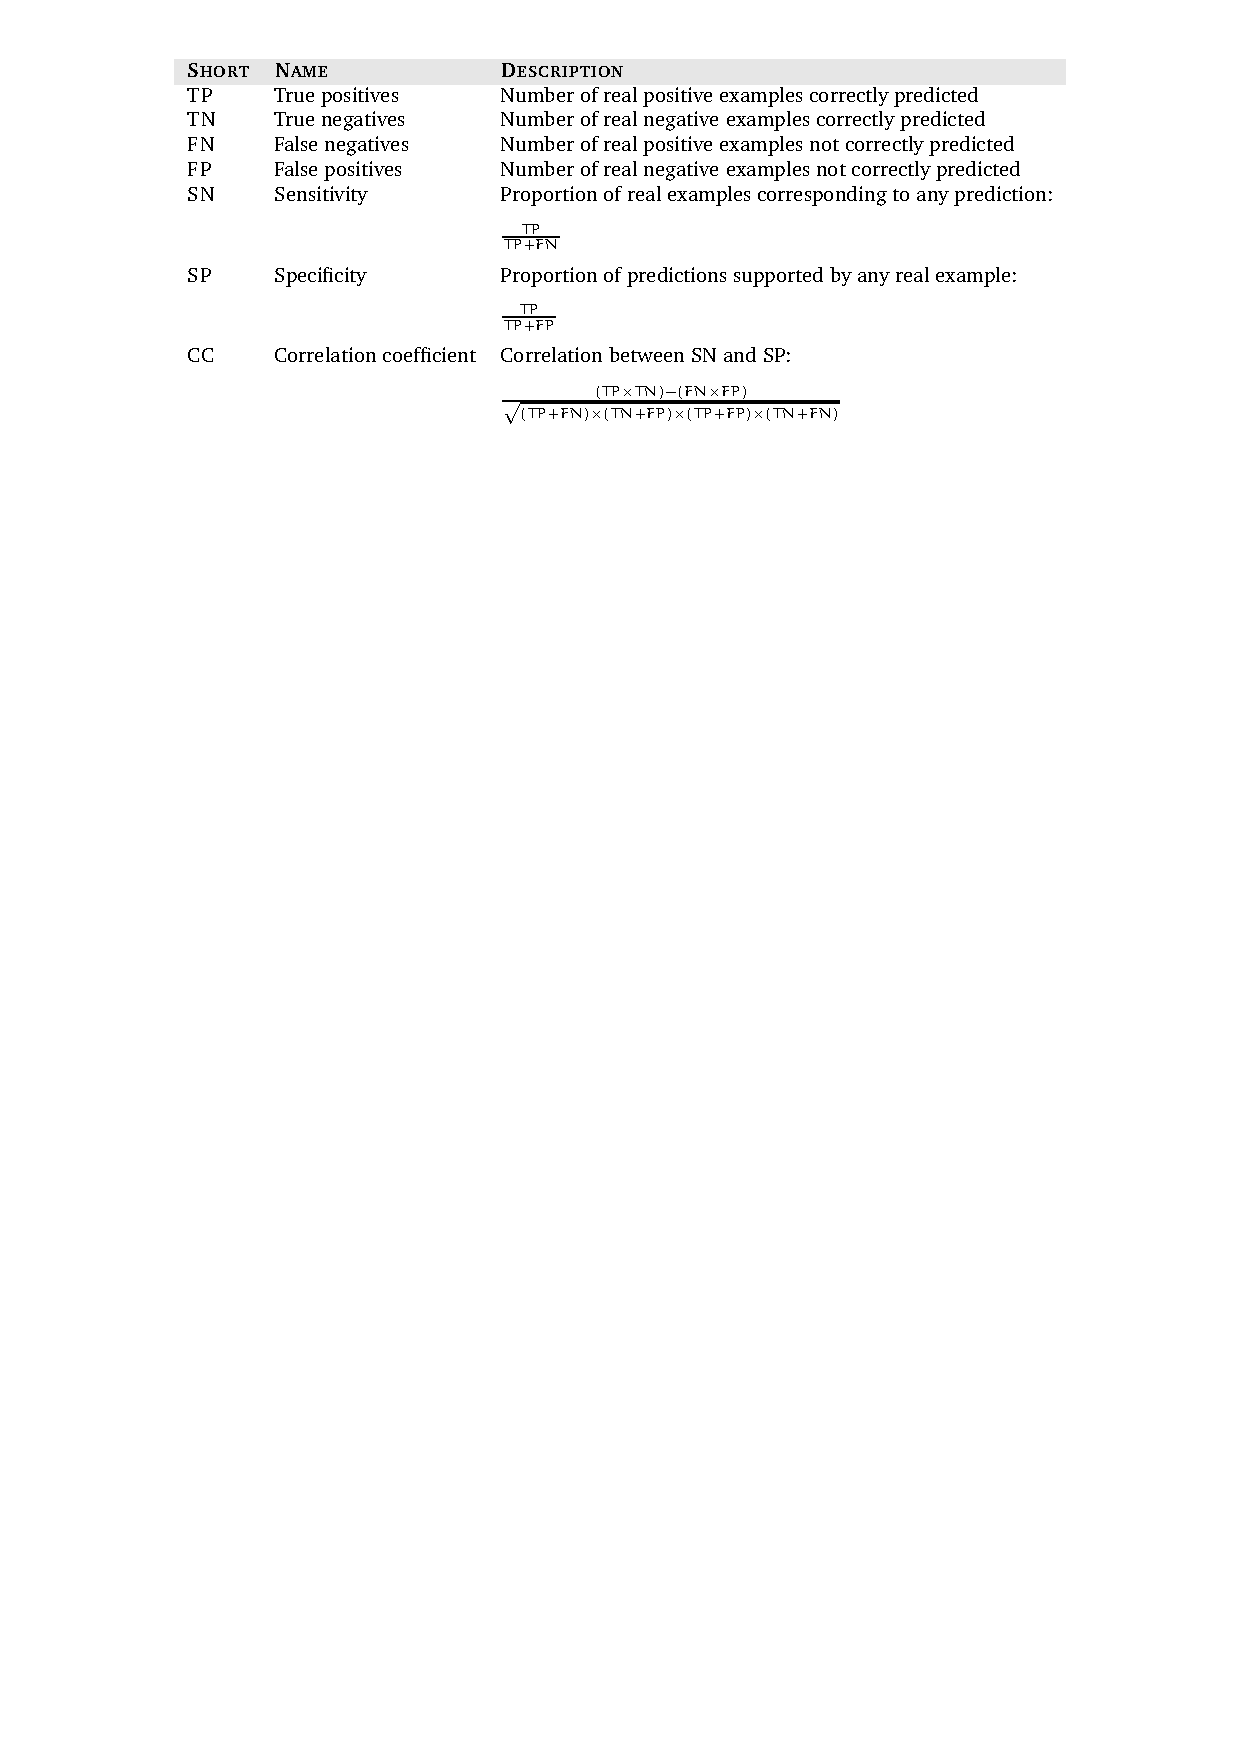
\includegraphics[bb=84 629 515 817,clip]{tables/accuracy}}
\end{center}
\end{minipage}
\mycaption{tab:accuracygenef}% label
          {The common accuracy measures in sequence analysis}% lof
          {The common accuracy measures in sequence analysis.}% caption header
          {}
\end{center}
\end{table}

Nowadays, after the completion of the first draft of the human genome 
we are completely immersed in a context of genomic research. The current generation 
of gene finders is devoted to the automatic reannotation of genomes by using the increasing 
amount of new information. Comparisons between genomes have proven to be very 
helpful in the discovery of novel genes \citep{guigo:2003a}. Some representatives
of the current generation of gene prediction programs are \prog{fgenesh+} 
\citep{salamov:2000a}, \prog{geneid} \citep{blanco:2003a} and \prog{genomescan} 
\citep{yeh:2001a}, or the comparative analysis systems \prog{doublescan} \citep{meyer:2002a}, 
\prog{rosetta} \citep{batzoglou:2000a}, \prog{slam} \citep{alexandersson:2003a}, 
\prog{sgp1} \citep{wiehe:2001a}, \prog{sgp-2} \citep{parra:2003a} 
and \prog{twinscan} \citep{korf:2001a}. 

The latest achievements in the sequencing of other higher eukaryotes have allowed the advent 
of comparative predictors that consider the alignment of multiple genomes in the prediction model, 
such as \prog{N-scan} that simultaneously combines the genomes of human, mouse, rat and 
chicken \citep{gross:2005a}. Moreover, new tools such as \prog{jigsaw} \citep{allen:2005a} and 
\prog{gaze} \citep{howe:2002a} for the assembly of data obtained from 
external sources of prediction and experimental evidence have been recently 
developed. 

\subsectionblue{\prog{geneid}}

\index{geneid}
The current version of \prog{geneid} \citep{blanco:2003a} is a program that predicts genes in anonymous 
genomic sequences designed following a simple hierarchical structure (see Figure \ref{fig:geneid} (A)). 
First, splice sites and start and stop codons are predicted and scored along the sequence. 
Next, potential exons are constructed from these sites and scored as the sum 
of the defining sites plus the score of a Markov model for coding DNA. Finally, 
from the set of predicted exons, the gene structure maximizing the sum of the 
score of its exons is assembled using a dynamic programming algorithm \citep{guigo:1998a}.

\prog{geneid} offers two features to integrate external information into the ab initio predictions: 
(1) sequence homology information can be used to reinforce the predictions that are supported by the 
alignment and (2) partial or complete genes obtained from other sources can be incorporated before 
the exon assembly.

As a consequence of its simple design, \prog{geneid} has been also parallelized.
Parallelism of data (distribution of data among processors with shared memory) was 
finally implemented because it was the best solution for distributing the
overload in the system. Following the divide and conquer strategy, the best gene 
structures computed in different processors are assembled introducing 
some overlap between sequence fragments (see Figure \ref{fig:geneid} (B)).

%%%%
% Figure 13: geneid + geneid parallel
%%%%
\begin{figure}[t!]
\begin{center}
\setlength{\fboxsep}{2pt}
\fbox{
\begin{tabular}{cc}
\incgraph{width=0.3\linewidth,height=6cm}{ps/geneid1} & 
\vspace{-1ex} \incgraph{width=0.55\linewidth,height=5cm}{ps/geneid2}\\
A & B \\
\end{tabular}}
\mycaption{fig:geneid}% label
          {\prog{geneid} dataflow}% lof
          {\prog{geneid} dataflow.}% caption header
          {(A) The serial dataflow. (B) The parallel dataflow.}
\end{center}
\end{figure}


The simplicity of the architecture of \prog{geneid} is appropriate to deal with
problems different from the canonical ones. Taking advantage of the implemented facilities to 
reannotate sequences, \prog{geneid} has been the main component of two recent genome annotation 
pipelines:

\begin{menumerate}
\item
Identification of novel selenoproteins in eukaryotes.\index{selenoproteins}
The presence of a secondary structure (SECIS element) in the 3' UTR of the mRNA induces the 
UGA codon, usually a termination signal, to be translated as Selenocysteine. \prog{geneid} was 
modified to permit the dual meaning of the UGA triplet, being succesfully applied to describe the 
\emph{Drosophila melanogaster}, human and \emph{Takifugu rubripes} selenoproteomes 
\citep{castellano:2001a, kryukov:2003a, castellano:2004a}. 
In addition, \prog{geneid} was used to reannotate selenoproteins in the \emph{Tetraodon nigroviridis} 
genome \citep{jaillon:2004a}, being the first eukaryotic genome project to integrate the 
identification of this particular family into the gene annotation pipeline.
\item
Comparative gene prediction.
\prog{sgp2} is a method to predict genes in a target genome sequence using the sequence of a
second informant or reference genome \citep{parra:2003a}. Essentially, \prog{sgp2} 
is a framework to integrate the search program \prog{tblastx} results with
\prog{geneid} predictions. The result of the \prog{tblastx} alignment of two sequences
is used by \prog{geneid} to rescore the exons supported by the alignment, 
penalizing the score of the others. \prog{sgp2} was successfully used in cooperation 
with another similar program called \ver{twinscan} \citep{korf:2001a} to discover 
a set of novel human and mouse genes. A subset of them was then experimentally 
validated in a subsequent stage of the genome comparison protocol \citep{guigo:2003a}.
The same protocol was used to annotate the genomes of human and chicken \citep{hillier:2004a}.
\end{menumerate}

\sectionorange{The state of the art in promoter characterization}

\index{promoter characterization!sta@state of the art}
The first algorithms of sequence alignment were enterely written to analyze proteins \citep{needleman:1970a}.
However, it was soon noticed that the same procedures could be applied over any type of biological
sequence, including transcription regulatory regions. For instance, \citet{sadler:1983a} used consensus 
and similarity searches to locate some general promoter elements in a set of vertebrate sequences. In 
\citep{waterman:1984d}, two algorithms to detect a common motif that can be known or unknown a priori 
in a set of sequences were presented. Later, these algorithms were used to characterize the 
core promoter of several \emph{Escherichia coli} genes \citep{galas:1985a}.

Consensus are a rudimentary form for representing regulatory sites so that new proposals to overcome their
limitations were published. \citet{staden:1984a} suggested the use of weight matrices. These PWMs were 
constructed from previous alignments of different types of biological sites. \citet{bucher:1990a}
systematically refined and tested the PWMs for detecting different regulatory 
signals such as the TATA box, the CAAT-box or the GC-box. At the same time, theoretical studies
to relate the information content and the quality of anchored alignments were already 
published \citep{schneider:1990a}. Posterior studies have shown the low specificity of the PWMs
when the set of initial examples is small \citep{schones:2005a}.

Soon, several databases to store the experimental examples and the constructed matrices were published, 
such as \db{Transfac} \citep{wingender:1988a}. At the same time, efficient programs to scan promoter 
sequences based on the pattern matching technique (pattern-driven approaches) were designed to use these 
matrices, being \prog{MatInspector} the most popular one \citep{frech:1993a,quandt:1995a}. However, methods 
to identify TFBSs in a single sequence demonstrated a very poor performance with an excess of false positives.
Certain improvements were observed when using additional information. New heuristic methods to discover 
unkown patterns in a set of regulatory sequences appeared (sequence-driven approaches): the application 
of the Gibbs sampling \citep{lawrence:1993a} and the expectation-maximization method \citep{bailey:1994a} 
are good examples. 

In general, however, the experimental investigation of a single promoter in all cell types where it can 
be active, under all conceivable conditions, at all possible developmental and cell-cyle stages, is 
in practice impossible. With this limitation in mind, the predictions obtained by any method must
be always very carefully evaluated to avoid the rejection of predicted functional sites that have not been 
experimentally annotated yet.

The identification of the core promoter regions and the annotation of the TSSs have also been two problems
associated to the problem of the TFBSs prediction. The presence of significantly over-expressed words or 
an unusual high percentage of CpG dinucleotides have traditionally been two measures of promoterness. 
For instance, \citet{davuluri:2001a} combined these two sensors with splicing detection to locate the first 
exon of a gene, predicting therefore the TSS position. Neural networks and genetic algorithms were used
in \citep{knudsen:1999a} to discriminate between promoter and non-promoter sequences. \citet{fickett:1997a}
reviewed the topic, showing the poor accuracy of most methods in the detection of the TSS. Word 
over-representations have been also used to study the 
association of adjacent TFBSs to form regulational modules or clusters with interesting results although 
the deciphering of a regulatory code seems still too complex \citep{beer:2004a,sharan:2003a,terai:2004a,thompson:2004a}. An example of such architectures is shown in Figure \ref{fig:modules}.

%%%%
% Figure 14: regulatory modules
%%%%
\begin{figure}[t!]
\begin{center}
\setlength{\fboxsep}{2pt}
\fbox{\incgraph{width=0.8\linewidth,height=6cm}{ps/modules}}
\mycaption{fig:modules}% label
          {Transcriptional regulatory module architectures}% lof
          {Transcriptional regulatory module architectures.}% caption header
          {Regulatory proteins and their gene targets are represented as blue circles and red boxes, respectively. Solid arrows indicate protein-DNA interactions, and genes encoding regulators are linked to their protein products by dashed lines. Adapted from \citep{harbison:2004a}.}
\end{center}
\end{figure}

A new revolution in the study of gene regulation began with the availability of genomic information and 
the possibility to work with abundant expression data. Phylogenetic footprinting, for instance, is a
new form of leaving a great fraction of false positives out \citep{duret:1997a,fickett:2000a}. 
Promising results have been obtained in several investigations \citep{blanchette:2002a,krivan:2001a,lenhard:2003a}. A review on phylogenetic footprinting can be found in \citep{wasserman:2004a}. 
Gene expression data from microarrays is the other great hope in the field to elaborate a regulatory map of 
human. Despite at the beginning, there was a boom of analysis of such data in different biological 
problems \citep{beltran:2003a,golub:1999a,shoemaker:2001a}, the difficulty to analyze and understand such 
an amount of data has been underscored in many occasions, though. The new generation of arrays based on 
chromatin immunoprecipitation promise to be an interesting method of prediction validation 
\citep{odom:2004a}. The combination of comparative genomics and expression data will become in a few years
the standard way to study a group of genes as in \citep{xie:2005a}.

Due to the poor results obtained when analyzing sequences to find pure binding motifs, intensive research 
has been performed in other areas to understand better the gene regulation problem. For instance, the 
association between CpG islands and promoters \citep{cuadrado:2001a}, DNA structure \citep{pedersen:1998a}, 
nucleosome positioning \citep{ioshikhes:1999a} or protein-DNA physical interactions \citep{halford:2004a}.

Similarly to the gene-finding accuracy tests, several assessments have been performed about the
quality of promoter characterization tools, always with discouraging results. The lack of stable
data sets of regulation sites, and the surprising difficulty to deal sometimes with orthologous sequences
are two causes that suggests the need for further improvement \citep{prakash:2005a,tompa:2005a}.

\sectionorange{Looking forward}

Despite the numerous advances in the basic algorithms of gene and promoter 
prediction and the unceasing flow of new data, the way to determine the exact number of 
genes in the human genome remains unclear \citep{pennisi:2003a} and the elaboration of a 
regulatory map of the human genome seems today an objective too ambitious \citep{wasserman:2004a}.

In the discipline of gene prediction, the same concepts have been applied since more than 20 years
ago. While the basic gene models have been improved to support comparative research, the definition
of a gene predicted by a gene-finder is still the same. It is true that some non-canonical gene 
structures are being slowly incorporated into the programs such as prediction of UTRs, alternative
splicing forms or selenoproteins \citep{brent:2004a}. Right now, the gene identification problem is 
still open and many efforts are engaged in the creation of a solid catalogue of human genes 
\citep{encode:2004a}, in which large-scale experimental methods of validation will be crucial \citep{brent:2005a}. 

Moreover, gene prediction and promoter recognition should be performed simultaneously. Unfortunately, 
we are far from reaching such an achievement due to the poor performance in the detection of regulatory elements 
despite the new and promising research that is currently being done in that direction \citep{pennacchio:2001a}.
The enormous volume of high-throughput expression data has provided new opportunities in the investigation of
the biology of the systems \citep{davidson:2002a}. Phylogenetic footprinting is also demonstrating their
capability to unveil regulatory blocks conserved in several species \citep{wasserman:2000a}. In addition, more accurate
catalogues of annotated regulatory elements are appearing, making the training of new pattern discovery methods
easier. All together will be part of a future pipeline to automatically identify and annotate the eukaryotic promoter 
regions. However, much effort must be still invested in understanding better other aspects of the same biological problem 
such as chromatin effect, methylation, or nucleosome movement \citep{pedersen:1999a}.

Perhaps a new line of thought should be established in both fields \citep{claverie:2000a}. So far, we have been only 
focusing on the sequence and many successful advances have been possible following such an approach. However, it is assumed that 
the cell machinery works in many levels with uncountable number of interactions that we have not incorporated 
in our systems yet. Once we have reached the limit with the current methods, and that moment is not too far, it will be 
essential to move from the current analytical systems to more constructive and dynamic applications, emulating
the mechanisms of the cell.

%%%%%%%%%%%%%%%%%%
%%% References for this chapter
%%% ENCERRAR ENTRE LLAVES PARA EVITAR PROBLEMAS
\bibliographystyle{plainnat}
{\bibliography{sections/bibliography}}
 % Gene-finding and promoter characterization
    \clearemptydoublepage

%%% BLOCK 3
\partgreen[Meta-Alignment of Sequences]{\textbf{M}eta-Alignment of Sequences}

    %%%%%%%%%%%%%%%%%%%%%%%%%%%%%%%%

% Meta-alignment of Biological Sequences

%%%%%%%%%%%%%%%%%%%%%%%%%%%%%%%%

\chapter[Meta-alignment of Biological Sequences]{\textbf{M}eta-alignment of\\ Biological Sequences}\label{sec:meta}
\sectiongreen*{Summary}
\begin{center}
\begin{tabular}{c}
\fcolorbox{blue}{verylightgrey}{
\begin{minipage}[][4cm][c]{0.8\linewidth}
\sffamily
%abstract 
This chapter contains the description of an efficient algorithm to align higher
order elements mapped over biological sequences. The relationship between
sequence alignments and meta-alignment is also reviewed. Such an approach 
is trained on a set of well annotated promoters. The ability of the meta-alignment 
to identify functional elements conserved at high level, such as regulatory elements
in co-regulated genes, in absence of sequence conservation is shown in several situations. 
In addition, the meta-alignment is used to evaluate the specificity of the weight matrices 
in a genome wide approach.
\end{minipage}}\\
\\[2ex]
\begin{minipage}[][4cm][c]{1.1\linewidth}
\minitoc
\end{minipage}
\end{tabular}
\end{center}
\newpage

\sectiongreen{Biological maps: promoters}\label{sec:}

\lettrine[lines=4,loversize=-0.1,lraise=0.1,lhang=.2]{S}{equence comparisons 
\index{sequence!seqcmp@sequence comparison} are among 
the most useful computational techniques} in molecular biology. Sequences of characters 
in the four-letter nucleotide alphabet and in the twenty-letter amino acid alphabet are 
extremely good symbolic representations of the underlying DNA and protein
molecules, and encode substantial information on their structure, function 
and history. 

Primary sequence comparisons, however, have limitations. Although 
similar sequences do tend to play similar functions, the opposite 
is not necessarily true. Often similar functions are encoded in
higher order sequence elements --such, for instance, structural motifs 
in amino acid sequences-- and the relation between these and the 
underlying primary sequence may not be univocal. As a result, similar 
functions are frequently encoded by diverse sequences.

As reviewed in Chapter \ref{sec:algorithms}, a biological map \index{maps}
is a description of functional objects (e.g. genes or regulatory sites) that are identified in a 
sequence at a given position. The annotation of the human genome in Figure \ref{fig:hgenome}
\index{genome!humgen@human genome} is a clear example of genomic mapping \index{genomic mapping} 
\citep{venter:2001a}. Comparison operations between maps are 
then necessary to elucidate functional relationships that are undetectable at the sequence level.

Promoter regions controlling eukaryotic gene expression are a case in
point. As reviewed in Chapter \ref{sec:genefinding}, the information for the control of the 
initiation of the gene transcription is mostly contained in the gene promoter, a region 
upstream of the gene transcription start site (TSS). Transcription factors
(TFs) interact in these regions with sequence specific elements or motifs 
(the TF binding sites, TFBSs). TFBSs are typically 5-15 nucleotides long and 
one promoter region usually contains many of them to harbor different TFs 
\citep{wray:2003a}. The interplay between these factors is not well understood, but the motifs 
appear to be arranged in specific configurations that confer on each gene an individualized
spatial and temporal transcription program \citep{wray:2003a}. It is
assumed, in consequence, that genes exhibiting similar expression
patterns would also share similar configurations of TFs in their
promoter.

However, TFBSs associated to the same TF are known to tolerate
sequence substitutions without losing functionality, and are often not
conserved.  Consequently, promoter regions of genes with similar
expression patterns may not show sequence similarity, even though they
may be regulated by similar configurations of TFs. For instance, only
about 30 to 40\% of the promoter regions are conserved between human
and chicken orthologous genes \citep{hillier:2004a}, and the
conservation of human-mouse orthologous promoter regions is only
slightly higher than that observed in intergenic regions
\citep{waterston:2002a}. Indeed, despite the recent progress due to the
development of techniques based in the so-called phylogenetic
footprinting, lack of nucleotide sequence conservation between functionally 
related promoter regions may partially explain the still limited success of 
current available computational methods for promoter characterization 
(see Chapter \ref{sec:genefinding} for a review of these methods).

%%%%
% Figure 1: the human genome is a map
%%%%
\begin{figure}[t!]
\begin{center}
\setlength{\fboxsep}{0pt}
\fbox{\incgraph{width=0.9\linewidth}{ps/hgenome}}
\mycaption{fig:hgenome}% label
          {The human genome map}% lof
          {The human genome map.}% caption header
          {This poster was produced with the program \prog{gff2ps} \citep{abril:2000a}. 
           Adapted from \citet{venter:2001a}.}
\end{center}
\end{figure}

In the approach described in this chapter \citep{blanco:2006b}, 
we attempt to overcome this limitation
by abstracting the nucleotide sequence, and representing a promoter
region by a sequence in a new alphabet in which the different symbols
denote different TFs. Using an external mapping function (for instance, 
a look-up table or a collection of position weight matrices, PWMs) that 
associates each TF to the nucleotide sequence motifs the factor is
known to bind, we can translate the nucleotide sequence of the
promoter into a sequence in this new alphabet. These sequences 
can be aligned. If the scoring of the
alignment takes into account not only the presence/absence of a given
symbol, but its relative position on the primary nucleotide sequence,
the optimal alignment between the promoter regions of two 
genes with similar expression patterns 
may reflect the underlying common configuration of
TFBSs.  We refer to these alignments either as meta-alignments, \index{meta-alignments}
as they are performed between sequences in a meta-alphabet, or map
alignments, since they are obtained after mapping the nucleotide
sequence in a higher order alphabet.

\sectiongreen{Transcription Factor maps}\label{sec:tfmaps}

Analogously to the restriction enzyme maps initially formalized by 
\citet{waterman:1984c} that are described in Chapter \ref{sec:algorithms},
we translate in our approach \citep{blanco:2006b} the nucleotide sequence 
of a promoter region $S = s_1 s_2 \ldots s_k$  into a sequence of 4-tuples
$A = a_1 \ldots a_n$ where each $a_i = <a_i^f,a_i^{p_1},a_i^{p_2},a_i^s>$
denotes the match with score $a_i^s$ of a binding site for the TF
$a_i^f$  occurring between the position $a_i^{p_1}$ and the position
$a_i^{p_2}$ over the sequence $S$. 

We obtain the translation from $S$ to $A$ by running on $S$ a collection of 
PWMs representing binding motifs for TFs (such as, for instance, the collection 
in \db{Transfac} \citep{matys:2003a}). For each match over a given threshold, we
register in $A$ the positions ($a_i^{p_1},a_i^{p_2}$), the score
($a_i^s$), and the label ($a_i^f$) of the TF associated to the PWM.
The translation preserves the order of $S$ in $A$, that is if $i < j$
in $A$ then $a_i^{p_1} \leq a_j^{p_1}$ (the $\leq$ is because matches
to different TFs may occur at the same position). We will refer to the
resulting sequence $A$ as a Transcription Factor Map (TF-map) 
\index{maps!tf@TF-maps} \index{TF-maps} or simply a map (see Figure 
\ref{fig:dummy}).  Note that other mapping functions, instead of
collections of PWMs, can also be used to translate $S$ into $A$.

In the implementation here, matches to PWMs are considered strandless,
that is, they are annotated at a given location, irrespective of the
orientation in which they occur. While biological evidence 
suggests that some TFBSs are functional only when present in a given 
strand, in other cases TF activity appears to be independent
of the orientation of the binding site \citep{strachan:1999a}. 
Since in general, we do not have information of
the strand in which a binding site may be functional, we have not
considered strand in our analysis.

\sectiongreen{TF-map pairwise alignment}\label{sec:TF-map alignment}

\index{TF-maps!alntf@alignments} \index{TF-map alignments} 
\index{alignment!tfma@TF-map alignments} \index{alignment!meta@meta-alignments}
The same types of sequence alignments that were reviewed in Chapter \ref{sec:algorithms} 
are also possible with maps: pairwise or multiple, global or local alignments. 
In this chapter, we described the algorithms of global and local pairwise TF-map alignment. 
The approach for multiple map alignment is detailed in the next chapter.

\clearpage
Formally, the pairwise alignment of the TF-maps $A = a_1 \ldots a_m$ and $B = b_1 \ldots b_n$ is a 
correspondence $T$, maybe empty, between $A$ and $B$ such that \citep{blanco:2006b}:
\begin{enumerate}

\item $(a_i,b_j) \in T$ if and only if $a_i^f = b_j^f$ (that is,
two elements are aligned if and only if they correspond to the same
TF). 

\item if $(a_i,b_j) \in T$ then there are no other elements $b_l~(l \neq j)$ in
$B$ such that $(a_i,b_l) \in T$, nor elements $a_k~(k \neq i)$ in $A$  such that
$(a_k,b_j) \in T$ (that is, each element in $A$ is aligned at most
to one element in $B$, and vice versa).

\item if $(a_i,b_j) \in T$ and $(a_k,b_l) \in T$ and $i<k$ then
$j<l$ (that is, the alignment maintains the colinearity between the
sequences $A$ and $B$).

\item if $(a_i,b_j) \in T$ and $(a_k,b_l) \in T$ with $i<k$ and $j<l$ then
$a_i^{p_2} < a_k^{p_1}$ and $b_j^{p_2} < b_l^{p_1}$ (that is, no overlap
in the primary sequences is permitted between the sites corresponding to the aligned elements).
\end{enumerate}

Usually there are many possible alignments between two given $A$ and
$B$ maps (see Figure \ref{fig:dummy} for an example). Given an alignment $T$

\begin{center}
\fcolorbox{white}{verylightgreen}{
\begin{minipage}[][][c]{0.95\linewidth}
\begin{equation}
T = \{ (a_{I_1},b_{J_1}), (a_{I_2},b_{J_2}), \cdots, (a_{I_t},b_{J_t}) \}
\end{equation}
\end{minipage}}
\end{center}

where $T_k = (a_{I_k},b_{J_k})$ is the match between the 4-tuple in position
${I_k}$ from A and the 4-tuple in position ${J_k}$ from B, we compute
the score of the alignment $s(T)$ in the following way:

\begin{center}
\fcolorbox{white}{verylightgreen}{
\begin{minipage}[][][c]{0.95\linewidth}
\begin{equation}
\begin{array}{ll}
s(T) = & \alpha \sum_{k=1}^t a_{I_k}^s + b_{J_k}^s\\
 & - \lambda (m + n -2 t)\\
%\sum_{k=2}^t (I_k - I_{k-1} - 1) + (J_k - J_{k-1} - 1) \\
 & - \mu \sum_{k=2}^t |(a_{I_k}^{p_1} - a_{I_{k-1}}^{p_1}) - (b_{J_k}^{p_1} - b_{J_{k-1}}^{p_1})|
\end{array}
\end{equation}
\end{minipage}}
\end{center}

where $\alpha, \lambda, \mu > 0$.
That is, the score of the alignment increases with the score of the
aligned elements ($\alpha$), and decreases with the number of
unaligned elements ($\lambda$), and with the difference in the distance 
between adjacent aligned elements ($\mu$).

%%%%
% Figure 2: TF-mapping and dummy TF-map alignment
%%%%
\begin{figure}[t!]
\begin{center}
\setlength{\fboxsep}{0pt}
\fbox{\incgraph{width=0.85\linewidth}{ps/dummy}}
\mycaption{fig:dummy}% label
          {TF-maps: construction and alignment}% lof
          {TF-maps: construction and alignment.}% caption header
          {(A) The sequence of a promoter is searched for occurrences of known
binding motifs for transcription factors (TFs). Matches are annotated with
the position of the match in the primary sequence, and the label of
the TF. Because TFs can bind to
motifs showing no sequence conservation, labels of the same
TF at different positions may correspond to
different underlying nucleotide sequences. We refer here to these
sequences of pairs (``label'', ``position''), transcription factor
maps (or TF-maps). TF-maps are actually more complicated. First, we do
not only register the position of each match, but also its
length. Second, while in the example here, sequence motifs
are associated to TFs by means of a (binary) look-up table, in our
work we have instead used collections of position weight
matrices. Matches to transcription factor binding sites (TFBSs) are thus
scored, and this score is also registered.
(B) TF-map of the promoter region of two hypothetically co-regulated genes
$X$ and $Y$.
Each letter corresponds to a different TF. We assume
that 200 nucleotides upstream of the annotated transcription start site 
(TSS) have been considered, with position 1 corresponding to position 
-200 from the TSS.
(C) Global pairwise alignment of the two co-regulated genes $X$ and $Y$. 
Only positions with identical labels can be aligned. Essentially, the 
alignment finds the longest common substring constrained to maximizing the 
sum of the scores (not shown here) of the aligned positions, and minimizing 
the differences in the distances on the primary sequence between 
adjacent aligned positions.}
\end{center}
\end{figure}

\subsectionblue{Finding the optimal alignment}

The optimal alignment between two given maps $A$ and $B$ is the
one scoring the maximum among all possible alignments. To obtain such
an alignment efficiently, we have implemented an algorithm reminiscent
of that proposed by \citet{waterman:1984c} to align and compare
restriction enzyme maps. This algorithm was developed to find the
distance between two homologous restriction maps in terms of minimum
weighted sum of genetic events necessary to convert one restriction
map into another, where the genetic events are the
appearance/disappearance of restriction sites and changes in the
number of bases between restriction sites (see Chapter \ref{sec:algorithms}
for further details).

Here to align TF-maps $A$ and $B$, we adapted the recursion in
\cite{waterman:1984c} to optimize similarity instead \citep{blanco:2006b}. In addition, we
included a term ($\alpha$) into the scoring function to weight the scores of the
TFBSs. We also explicitly prohibited overlap between the sites.

Thus, the maximum similarity $S_{ij}$ between TF-maps  $A = a_1 \ldots a_i$ and 
$B = b_1 \ldots b_j$ where the site $a_i^f$ is equal to the site $b_j^f$, 
can be computed as: 

\begin{center}
\fcolorbox{white}{verylightgreen}{
\begin{minipage}[][][c]{0.95\linewidth}
\begin{equation}
\begin{array}{llll}
S_{ij} \equiv & S(a_i,b_j) = & \alpha (a_i^s + b_j^s) +& \\
              & &  max_{i',j'} & \{S_{i'j'}\\
              & & \scalebox{0.7}{\mbox{$0 < i' < i$}} & - \lambda (i - i' - 1 + j - j'- 1)\\
              & & \scalebox{0.7}{\mbox{$0 < j' < j$}} & - \mu (|(a_i^{p_1} - a_{i'}^{p_1}) - (b_j^{p_1} - b_{j'}^{p_1})|)\}.\\
              & & \scalebox{0.7}{\mbox{$a_{i'}^{p_2} < a_i^{p_1}$}} & \\
              & & \scalebox{0.7}{\mbox{$b_{j'}^{p_2} < b_j^{p_1}$}} &  
\end{array}
\end{equation}
\label{eqnaive}
\end{minipage}}
\end{center}

\subsectionblue{Sequence alignments and meta-alignments}

\index{TF-map alignments!seqaln@sequence alignments} \index{alignment!seqtf@sequences and TF-maps}
There is an intimate relationship between the Equation \ref{eqnaive} and the Needleman
and Wunsch recurrence as revisited by \citet{smith:1981b} in which the conventional pairwise 
sequence alignment is based (see Chapter \ref{sec:algorithms}, Section \ref{nwrevisited}).

In fact, the sequence alignment class of algorithms are a particular case of the
more general class of map alignment algorithms. Let us analyze the form in which
the conventional sequence alignment calculates any value in the similarity matrix $S$, trying
to detect for each element in such a recurrence its counterpart in Equation \ref{eqnaive}:

\begin{menumerate}
\item
The matches and the substitutions between two symbols $x$ and $y$ are assigned the value 
of the corresponding scoring function $s(x,y)$ in a sequence alignment. The matches between
two elements in a meta-alignment are also scored using a similar function (the $\alpha$ 
parameter in Equation \ref{eqnaive}). Let us consider $\alpha=(\alpha_1,\alpha_2 \ldots \alpha_k)$
the family of scoring functions for evaluate any type of identity and substitution between two
symbols $x$ and $y$. If the mapping quality score of each element is omitted, the scoring functions 
$s$ and $\alpha$ are equivalent.
\item
The number of gaps in a sequence alignment is punished by the scoring function $s(x,-)=s(-,x)$. 
There is not an explicit penalty for introducing a single gap into a meta-alignment. However, 
the $\lambda$ parameter punishes the number of elements in two maps that are not included
in the optimal met-alignment. Because such unaligned elements are implicitly aligned to gaps in 
the other map, the $\lambda$ parameter is the equivalent of the scoring function $s(x,-)$.
\item
The $\mu$ parameter must be silenced due to the lack of mapping information in conventional sequences. 
\end{menumerate}

A trivial mapping function to translate a sequence of nucleotides into a map that can be meta-aligned
consists on using the position of the elements in the sequence also as the position in the map. 
The length of every feature is in this case one position. The score of each feature is neglected
as nucleotides do not have this value. With these considerations in mind, the sequence of nucleotides 
$S=ATTACTG$ can be transformed into the map $M$:

\begin{center}
\fcolorbox{white}{verylightgreen}{
\begin{minipage}[][][c]{0.95\linewidth}
$$%\begin{equation}
\begin{array}{lccccccc}
S: & A & T & T & A & C & T & G\\[2ex]
M: & (A,1,1,\cdot) & (T,2,2,\cdot) & (T,3,3,\cdot) & (A,4,4,\cdot) & (C,5,5,\cdot) & (T,6,6,\cdot) & (G,7,7,\cdot).\\
\end{array}
$$%\end{equation}
\end{minipage}}
\end{center}

The meta-alignment class of algorithms can deal, therefore, with any sequence alignment problem.
However, the opposite is not true, as meta-alignments involve management of higher-order level
features that are not supported in the classical sequence comparisons.


\subsectionblue{Naive implementation}
\index{TF-map alignments!naive@naive algorithm} \index{algorithms!tfnaive@TF-map alignment}
A naive implementation of the recursion above (Equation \ref{eqnaive}) involves
the recursive filling of the cells $S_{ij}$ in the matrix $S$ \citep{waterman:1984c}. 
In the pseudocode shown in Figure \ref{fig:naivealg}, the elements of the maps $A$ and $B$ are represented as 
structures $a_i$ and $b_j$, with the functions \emph{factor}, \emph{score}, \emph{pos1} 
and \emph{pos2} returning the values of the corresponding fields. The variable 
\emph{currentSim} stores the optimal score so far computed. The resulting meta-alignment 
can be easily retrieved using a supplementary structure \emph{path(i,j)} which points to 
the previous cell in the optimal path leading to cell $S_{ij}$. In addition, for each 
cell $S_{ij}$, the function \emph{ComputeInitialSimilarity} calculates the initial score of 
a hypothetical alignment that includes only $a_i$ and $b_j$.

Note that to compute the optimal score at $S_{ij}$ with this algorithm, 
all the cells $S_{kl}$ ($k<i$, $l<j$) need to be explored (see Figure \ref{fig:naivealg}). 
Therefore, if the lengths of the TF-maps $A$ and $B$ are $m$ and $n$ respectively, the 
cost of computing $S(A,B)=S(a_m,b_n)$ is $O(mn \cdot mn) = O(m^2n^2)$. 
Under the assumption that $m$ and $n$ are similar lengths, the final cost 
function is $O(n^4)$.


%%%%
% Figure 3: Naive algorithm
%%%%
\begin{figure}[t!]
\begin{center}
\scalebox{1}{
\fcolorbox{white}{verylightgreen}{
\begin{minipage}[][][c]{0.95\linewidth}
\begin{algorithmic}[5]
 \REQUIRE $A,B$: list of $<$factor,pos1,pos2,score$>$
\STATE \COMMENT{Calculating the element $i,j$ in $S$}
\FOR{$i=0$ to $|A|-1$}
\FOR{$j=0$ to $|B|-1$}
\IF{factor$(a_i)$ = factor$(b_j)$}
\STATE $S(i,j) \leftarrow$ ComputeInitialSimilarity();
\STATE $x \leftarrow \alpha$ (score$(a_i)$ + score$(b_j)$);
\STATE \COMMENT{Searching the best previous match in $S$}
\FOR{$i'=0$ to $i-1$}
\FOR{$j'=0$ to $j-1$}
\IF{pos2($a_{i'}$) $<$ pos1($a_i$) and pos2($b_{j'}$) $<$ pos1($b_j$)}
\STATE $y \leftarrow \lambda ((i-i'-1) + (j-j'-1))$;
\STATE $z \leftarrow \mu (|($pos1$(a_i)$ - pos1$(a_{i'})$) - (pos1$(b_j)$ - pos1$(b_{j'}))|)$;
\STATE currentSim $\leftarrow S(i',j') + x - y - z$;
\IF{currentSim $> S(i,j)$}
\STATE $S(i,j) \leftarrow$ currentSim; 
\ENDIF
\ENDIF
\ENDFOR
\ENDFOR
\ENDIF
\ENDFOR
\ENDFOR
\end{algorithmic}
\begin{center}
%\fbox{
\incgraph{width=0.75\linewidth}{ps/prev}%}
\end{center}
\end{minipage}}}
\mycaption{fig:naivealg}% label
          {The Naive TF-map alignment algorithm}% lof
          {The Naive TF-map alignment algorithm.}% caption header
          {The whole matrix must be visited for each new match $S_{ij}$}
\end{center}
\end{figure}

\subsectionblue{Enhanced implementation}

\index{TF-map alignments!enh@enhanced algorithm} \index{algorithms!tfnaive@TF-map alignment}
\citet{myers:1992a} described an improved algorithm for computing in
$O(mn(\log m + \log n))$ time the minimum distance between two
restriction maps of length $m$ and $n$ respectively under the original
framework proposed by \citet{waterman:1984a}. The algorithm, reviewed
in Chapter \ref{sec:algorithms}, is basically a sparse dynamic programming 
computation in which candidate lists are used to model the future contribution 
of all previously computed cells in distance matrix $D$ to those yet to be computed.
The cells in the list that can not affect the values of any cell to be
computed are eliminated from the list. The key concept of this
algorithm is the mapping of the original matrix $D$ to another matrix
in which each cell is indexed by the positions of the sites in 
the original sequences, and not by their positions in the maps. 
During the computation, this matrix is partitioned into intervals for which
only a representative cell is used to compute the best alignment
ending at each match in a given interval.

Here, we can not directly export this strategy, because, in contrast
to the restriction enzyme maps which are points in the sequence, TFBSs 
are sequence intervals (having, thus, two dimensions). In addition,
different TFBSs can start at the same point, but end at different
positions. Since we explicitly prohibit overlapping between TFBSs in the
alignments, the assignation of a cell representative within a given
interval must not be irreversible. 

However, we have still taken advantage of the extreme sparsity of the
matrix $S$ when aligning TF-maps \citep{blanco:2006b}. Note that, in general, the
probability of matching two elements from two sequences of characters
that follow a uniform random distribution is inversely proportional to
the size of the character alphabet.  For instance the probability of
matching two nucleotides when comparing two random DNA sequences in
the four letter alphabet is about 0.25. In an alphabet of about 100
characters --the order of magnitude of the alphabets of symbols denoting
TFs that we are considering here-- such a probability would be
about 0.01. When aligning sequences in alphabets of such sizes, the
matrix $S$ above, that only takes values for match positions between
$A$ and $B$, becomes therefore extremely sparse. Indeed, Figure 
\ref{fig:sparsem} displays the occupancy of the matrix $S$ corresponding
to the alignments of the TF-maps obtained on the human and mouse
promoters of the \emph{skeletal muscle $\alpha$-actin} gene (ACTA1, GenBank
entries AF182035 and M12347). We have used three different collections
of PWMs for TFBSs (see next section) to obtain the TF-maps of both
promoter sequences. In all cases, despite the differences in the
lengths of the obtained maps, the occupancy of the matrix $S$ is well
under 5\%.

%%%%
% Figure 5: Sparse matrices
%%%%
\begin{figure}[t!]
\begin{center}
\setlength{\fboxsep}{0pt}
\begin{tabular}{ccc}
\incgraph{width=0.25\linewidth}{ps/sparsem1} &
\incgraph{width=0.25\linewidth}{ps/sparsem2} &
\incgraph{width=0.25\linewidth}{ps/sparsem3}\\
\end{tabular}
\mycaption{fig:sparsem}% label
          {Sparse matrices}% lof
          {Graphical representation of the sparse dynamic programming matrix $S$.}% caption header
          {Matrices produced by the transcription factor map alignment between the human 
           and mouse promoters of the \emph{skeletal alpha-actin} gene (ACTA1,
           GenBank entries AF182035 and M12347), using different collections of 
           position weight matrices for transcription factor binding sites (TFBSs). 
           The axes of the matrix list the transcription factor labels of the predicted
           TFBSs in the human and mouse promoters. Despite the differences in the 
           total number of predicted TFBSs depending on the collection, the occupancy 
           of the matrix remains consistently low.}
\end{center}
\end{figure}

In the algorithm presented in Figure \ref{fig:enhancedalg}, we substitute the two internal nested 
loops by a list $L$ to register the coordinates of the match cells in the sparse matrix $S$. 
Each node of $L$ is represented as structures $p$ and $n$ with the functions
\emph{abscissa} and \emph{ordinate} returning the corresponding coordinates.
Thus, to compute the optimal score at the cell $S_{ij}$, only the non-empty cells 
in $S$ need to be accessed. In addition, we maintain the list sorted 
by optimal score, so that the cell scoring the maximum value is at the beginning of 
the list. Scanning the list from the beginning to the end implies that, in most cases, 
only a few nodes will need to be accessed before a a critical node is reached 
beyond which the optimal score can not be improved.

While investigating the exact complexity of this algorithm is
difficult --depending mostly on the size of the input maps and the
sparsity of the resulting matrix $S$--, the expected time cost analysis
can be performed. The $O(n^4)$ cost of the naive algorithm can be
explained in terms of (a) a first quadratic term derived from the
obligatory comparison between all of the TFBSs of both maps to detect
the match cells and (b) a second quadratic term necessary to search
for each match the best adjacent previous pair in the optimal TF-map
alignment.

%%%%
% Figure 6: Enhanced algorithm
%%%%
\begin{figure}[t!]
\begin{center}
\scalebox{1}{
\fcolorbox{white}{verylightgreen}{
\begin{minipage}[][][c]{0.95\linewidth}
\begin{algorithmic}[5]
\REQUIRE $A,B$: list of $<$factor,pos1,pos2,score$>$, $L$: list of $<$abscissa,ordinate$>$, $L = \emptyset$ 
\STATE \COMMENT{Calculating the element $i,j$ in $S$}
\FOR{$i=0$ to $|A|-1$}
\FOR{$j=0$ to $|B|-1$}
\IF{factor$(a_i)$ = factor$(b_j)$}
\STATE $S(i,j) \leftarrow$ ComputeInitialSimilarity();
\STATE $x \leftarrow \alpha$ (score$(a_i)$ + score$(b_j)$);
\STATE \COMMENT{Searching the best previous match in $L$}
\STATE $p \leftarrow$ first($L$);
\STATE $i' \leftarrow$ abscissa($p$);
\STATE $j' \leftarrow$ ordinate($p$);
\WHILE{end($L$) = FALSE and $S(i',j') + x > S(i,j)$}
\IF{pos2($a_{i'}$) $<$ pos1($a_i$) and pos2($b_{j'}$) $<$ pos1($b_j$)}
\STATE $y \leftarrow \lambda ((i-i'-1) + (j-j'-1))$;
\STATE $z \leftarrow \mu (|($pos1$(a_i)$ - pos1$(a_{i'})$) - (pos1$(b_j)$ - pos1$(b_{j'}))|)$;
\STATE currentSim $\leftarrow S(i',j') + x - y - z$;
\IF{currentSim $> S(i,j)$}
\STATE $S(i,j) \leftarrow$ currentSim; 
\ENDIF
\ENDIF
\STATE $p \leftarrow$ next($L$);
\STATE $i' \leftarrow$ abscissa($p$);
\STATE $j' \leftarrow$ ordinate($p$);
\ENDWHILE
\STATE $n \leftarrow$ CreateNewNode($i,j$);
\STATE InsertNode($n,L$);
\ENDIF
\ENDFOR
\ENDFOR
\end{algorithmic}
\end{minipage}}}
\mycaption{fig:enhancedalg}% label
          {The Enhanced TF-map alignment algorithm}% lof
          {The Enhanced TF-map alignment algorithm.}% caption header
          {}
\end{center}
\end{figure}

In this enhanced algorithm, the contribution (a) is inevitable so that
the lower bound of the cost function is the number of matches between
both TF-maps, that is $O(n^2)$. However, the substitution of the two
inner loops for a list of cell matches sorted by optimal score does
affect the contribution (b). Thus, such a term is now equivalent to the expected
number of consulted elements of the ordered list $L$ to compute each $S_{ij}$ value.
This expectation can be approximated to

\begin{center}
\fcolorbox{white}{verylightgreen}{
\begin{minipage}[][][c]{0.95\linewidth}
\begin{equation}
O\left(~\sum_{\alpha\in {\cal A}} (P(\alpha)^2 n^2)~\right)
\end{equation}
\end{minipage}}
\end{center}

where ${\cal A}$ is the set of symbols (in our case the alphabet of TFs) and
$P(\alpha)$ is the probability to match the symbol $\alpha$ in a random trial
(it is a particular case of the sequence comparison by hashing,
see Theorem 8.1 in \cite{waterman:1995a}). Therefore, under the previous 
hypothesis of a comparison between two TF-maps in an alphabet of $100$ characters 
that follows a uniform random random distribution ($P(\alpha) = 0.01$, 
only 1\% of the matrix is occupied), the expected value of the contribution (b) 
is $O(0.01~n^2)$. 

The empirical results obtained during the program training (see next section)
confirmed such analysis \citep{blanco:2006b}. In average, on the order of 200 
million elements were consulted by the naive algorithm during the optimization. 
In contrast, the enhanced algorithm only needed to access nearly two million elements 
to compute the same set of alignments (see Figure \ref{fig:access}).

\clearpage
%%%%
% Figure 7: Access to the matrix S
%%%%
\begin{figure}[t!]
\begin{center}
\setlength{\fboxsep}{0pt}
%\fbox{
\incgraph{width=0.75\linewidth}{ps/access}%}
\mycaption{fig:access}% label
          {Number of accessions to the matrix $S$}% lof
          {Number of accessions (in millions) to the matrix $S$.}% caption header
          {In red, the performance of the Naive algorithm; in orange, the performance
           of the Enhanced algorithm, with a normal list $L$; in green, the performance
           of the Enhanced algorithm, sorting the list $L$.}
\end{center}
\end{figure}

\sectiongreen{TF-map alignment training}\label{sec:TF-map training}
\index{TF-map alignments!trai@training} \index{meta-alignments!mtrai@training} 
The optimal alignment between two TF-maps is obviously
dependant on the $\alpha$, $\lambda$, and $\mu$ parameters. In
principle, we want the optimal alignment between the maps derived from
promoter sequences of two co-expressed genes to include most of the
mapped TFBSs known to be involved in the regulation of the genes (high
sensitivity), and few of the mapped TFBSs not known to be involved in such
regulation (high specificity). The implicit assumption here is that
the TFBSs in the alignment are considered predictions of TFBSs on the
underlying promoter sequences. It is also important to stress that two
different TFBSs can be aligned if they correspond to the same TF.

The optimal parameter configuration, however, is likely
to depend on the particular problem to be addressed: the genes to be
compared (orthologous genes from different species or genes
co-regulated after an expression microarray experiment, for instance),
and the particular protocol to map the TFBSs into the original promoter
sequences. Often the optimal configuration of parameters will be
specific of the pair of gene promoters to be compared. 

With these caveats in mind, since our focus here is on mammalian comparisons,
we have estimated the parameters that are globally optimal when aligning a set of well
annotated human-mouse orthologous promoter pairs \citep{blanco:2006b}. The underlying
assumption is that these orthologous pairs are regulated in a
similar way. We have estimated the optimal parameters separately 
in three different collections of PWMs for locating TFBSs,
and in each case we have chosen the parameters such that the resulting 
global alignment achieved the maximum average sensitivity and specificity as 
defined below.

\subsectionblue{Datasets}

\index{TF-map alignments!traidata@training datasets} 
From several landmark papers in the field
\citep{wasserman:1998a,krivan:2001a,blanchette:2002a,dermitzakis:2002a,lenhard:2003a}, 
we have gathered and manually curated a collection of 278 TFBSs (139 +
139 orthologous sites) that had been experimentally tested in 40
orthologous human and rodent genes. The transcription start site (TSS)
of each entry in the literature was compared to the RefSeq \citep{pruitt:2005a}
annotation of the corresponding genome to ensure that we were dealing with the
actual proximal promoter. Because most (214 out of 278) of
the annotated TFBSs are located in the 200 nucleotides immediately
upstream of the TSS, we restricted to this region in our training and
evaluation analysis, and considered only those cases for which the
same pair of TFBSs had been annotated in this region for both species. 
This resulted in a collection of 202 sites (101 + 101)
from 36 genes, to which we refer here as the \textsc{HR set}.

We have estimated the optimal parameters in the \textsc{HR set} for the \db{Jaspar} 1.0, 
\index{JASPAR} \db{Promo} 2.0 \index{PROMO} and \db{Transfac} 6.3 collections. \index{TRANSFAC}
In the three cases, the original frequency coefficients of the matrices have been
converted into log-likelihood ratios using the random equiprobability 
distribution as a background model. The log operation can not be directly
performed on matrix positions containing null values (that is, 0 occurrences).
We have instead estimated the value of the log-likelihood function for the null positions 
in a given matrix row, taking into account the values computed in that row for 
one and two occurrences. Let $y = f(x)$ be the log-likelihood function 
approached as a line that goes from the point $P=(x_1,y_1)$ to the point 
$Q=(x_2,y_2)$. If we consider $P=(x_1,1)$ and $Q=(x_2,2)$ 
which correspond to the cases in which one and two occurrences are present,
the values $x_1$ and $x_2$ can be easily computed. Thus, the equation of the
line that goes from $Q$ to $P$ can be inferred for each row of the matrix.
In particular, the value of this line in the point $R=(x_0,0)$ can be
trivially calculated, being used as an estimation for the null values in
that row of the matrix. 

Let $M$ be a PWM constructed from $33$ TFBSs, where $M_i$ and $M_i^*$ denote the 
absolute and relative frequency of each nucleotide at the position $i$, respectively. The
conversion from $M_i$ into a log-likelihood ratio matrix is explained in the 
following example (base-$e$ logarithms):

\begin{center}
\fcolorbox{white}{verylightgreen}{
\begin{minipage}[][][c]{0.95\linewidth}
%\begin{equation}
$$
\begin{array}{rrrrr}
    & A &  C & G & T\\[2ex]
M_i & 7 & 25 & 0 & 1\\[2ex]
M_i^* = \frac{M_i}{33} & 0.21 & 0.75 & 0 & 0.03\\[2ex]
\log{\frac{M_i^*}{0.25}} & -0.164 & 1.109 & ? & -2.110\\[2ex]
Estimation & & & -2.803 & \\
\end{array}
$$
%\end{equation}
\end{minipage}}
\end{center}

The resulting matrices were used to obtain the list of TFBSs matches 
along the 200 bases upstream of the TSS in each of the 36 pairs of promoter 
sequences from the \textsc{HR set}. A prediction obtained with a given PWM 
was accepted if it had an score above the 50\% (\db{Jaspar}), 70\% (\db{Promo}) and 55\%
(\db{Transfac}) of the maximum possible score for such PWM. These values
correspond in the three cases to the conventional 80\% threshold when
considering the original frequency matrices \citep{blanco:2006b}. 

Those annotated TFBSs not included in the predictions for both
orthologous pairs (either because no matrix exists in the collection
for such TFBSs, or because the match is below the threshold) were discarded. 
This reduced the effective number of training gene pairs (those with at least
one real predicted TFBS for both orthologous pairs) from 36 to 29 for the 
three collections considered here \citep{blanco:2006b}.

Table \ref{tab:accuracy} shows for each collection the total number of matrices, 
and TFs to which they correspond, the number of genes for which at least one 
annotated TFBS is predicted on each ortholog after the search, and the number 
of real and predicted TFBSs (the total and the average per gene pair). As it 
is possible to see, slightly more than three conserved TFBSs were annotated per
orthologous gene pair \citep{blanco:2006b}. 

\subsubsectionblue{Collecting regulatory data}

Information about the genomic coordinates and the sequence of experimentally 
identified transcription factor binding sites is found scattered under a variety 
of diverse formats. The availability of standard collections of such high-quality 
data is important to design, evaluate and improve novel computational approaches to 
identify binding motifs on promoter sequences from related genes. 

Typically, computational methods to detect regulatory elements use their own training 
set of experimental annotated TFBSs. These annotations are usually collected from 
bibliography or from general repositories of gene regulation information, such as 
\db{Jaspar} \citep{sandelin:2004a} or \db{Transfac} \citep{matys:2003a}. However, each program 
establishes different criteria and formats to retrieve and display the data that forms 
the final training set, which makes the comparison between different methods very 
difficult. The construction of a good benchmark to evaluate the accuracy of several 
pattern discovery methods is therefore not a trivial procedure \citep{tompa:2005a}.

To build the TF-map alignment training dataset, we gathered from the literature a 
collection of experimentally validated binding sites that are conserved in at least
two orthologous vertebrate promoters. The sites and the promoter 
sequences were manually curated to ensure data consistency. The data is publicly
available at the \db{ABS} database (see Web Glossary). \index{ABS} 

We annotated in \db{ABS} \citep{blanco:2006a} up to 650 
experimental binding sites from 68 transcription factors and 100 orthologous target 
genes in human, mouse, rat or chicken genome sequences. Computational predictions 
and promoter alignment information are also provided for each entry. In addition, 
we provided a web interface to interact and analyze the promoters and their binding 
sites (see Figure \ref{fig:absweb}). We also included a customizable generator of artificial 
datasets and an evaluation tool to aid during the training of motif-finding programs 
\citep{blanco:2006a}.


\subsectionblue{Accuracy measures}

After the maps were obtained, we aligned them within each orthologous
pair using the algorithm described in the previous section with
different combinations of parameters. Each parameter was allowed to
independently take values between 0.0 and 1.0, in incremental steps of
0.01.  In total, thus, one million parameter configurations were
evaluated for each collection of PWMs.  For each configuration,
the resulting optimal alignments on the pairs of orthologous promoters
(that is, the predicted TFBSs) were compared to the annotated TFBSs in
the promoters.

Two values were computed to measure the agreement between predicted
and annotated TFBSs: sensitivity and specificity. Sensitivity
is the number of correctly predicted TFBSs over the number of
annotated TFBSs, and specificity is the number of correctly predicted TFBSs
over the number of predicted TFBSs. We used here the term specificity as 
in the gene finding literature. However, the value that we compute here 
is more generally known as Positive Predictive Value. We considered an 
annotated TFBS to be correctly predicted when there was a predicted TFBS that 
overlapped it by at least 1 nucleotide in both human and mouse sequences,
irrespectively of whether the TF label associated to the aligned TFBS
matched that of the annotated TFBS. This is because TFBSs for different 
TFs often cluster at the same position when using PWMs (see Figure 
\ref{fig:pspla}). If a similar cluster occurs in the two sequences to be
aligned, our algorithm will inevitably choose to align the pair of
TFBSs with the highest sum of match scores.

As an optimization measure we computed the average value of sensitivity
and specificity. Table \ref{tab:accuracy} lists the optimal combination of 
parameters with regard to this measure for each of the three collections of 
PMWs used here. Table \ref{tab:accuracy} also lists sensitivity, specificity, their average, 
the average length of the optimal alignments (that is, the number of predicted 
TFBSs after the alignment), and the fraction of the promoter region covered by the
predicted (aligned) TFBSs. In addition, for each optimal configuration
we have also computed the same set of accuracy measures under the
strict criterion of considering an annotated TFBS to be correctly
predicted only when the TF label of the prediction matched that of the
overlapped annotation. We also computed sensitivity and specificity at 
the nucleotide level. At this level, we compute the number of nucleotides in
predicted TFBSs that are also in annotated TFBSs. 

%%%%%%%%%%%%%%%
%%% TABLE 1
%%%%%%%%%%%%%%%
\begin{landscape}
\begin{table}[t!]
\begin{center}
\begin{minipage}{0.98\linewidth}\setlength{\parindent}{0pt}
\begin{center}
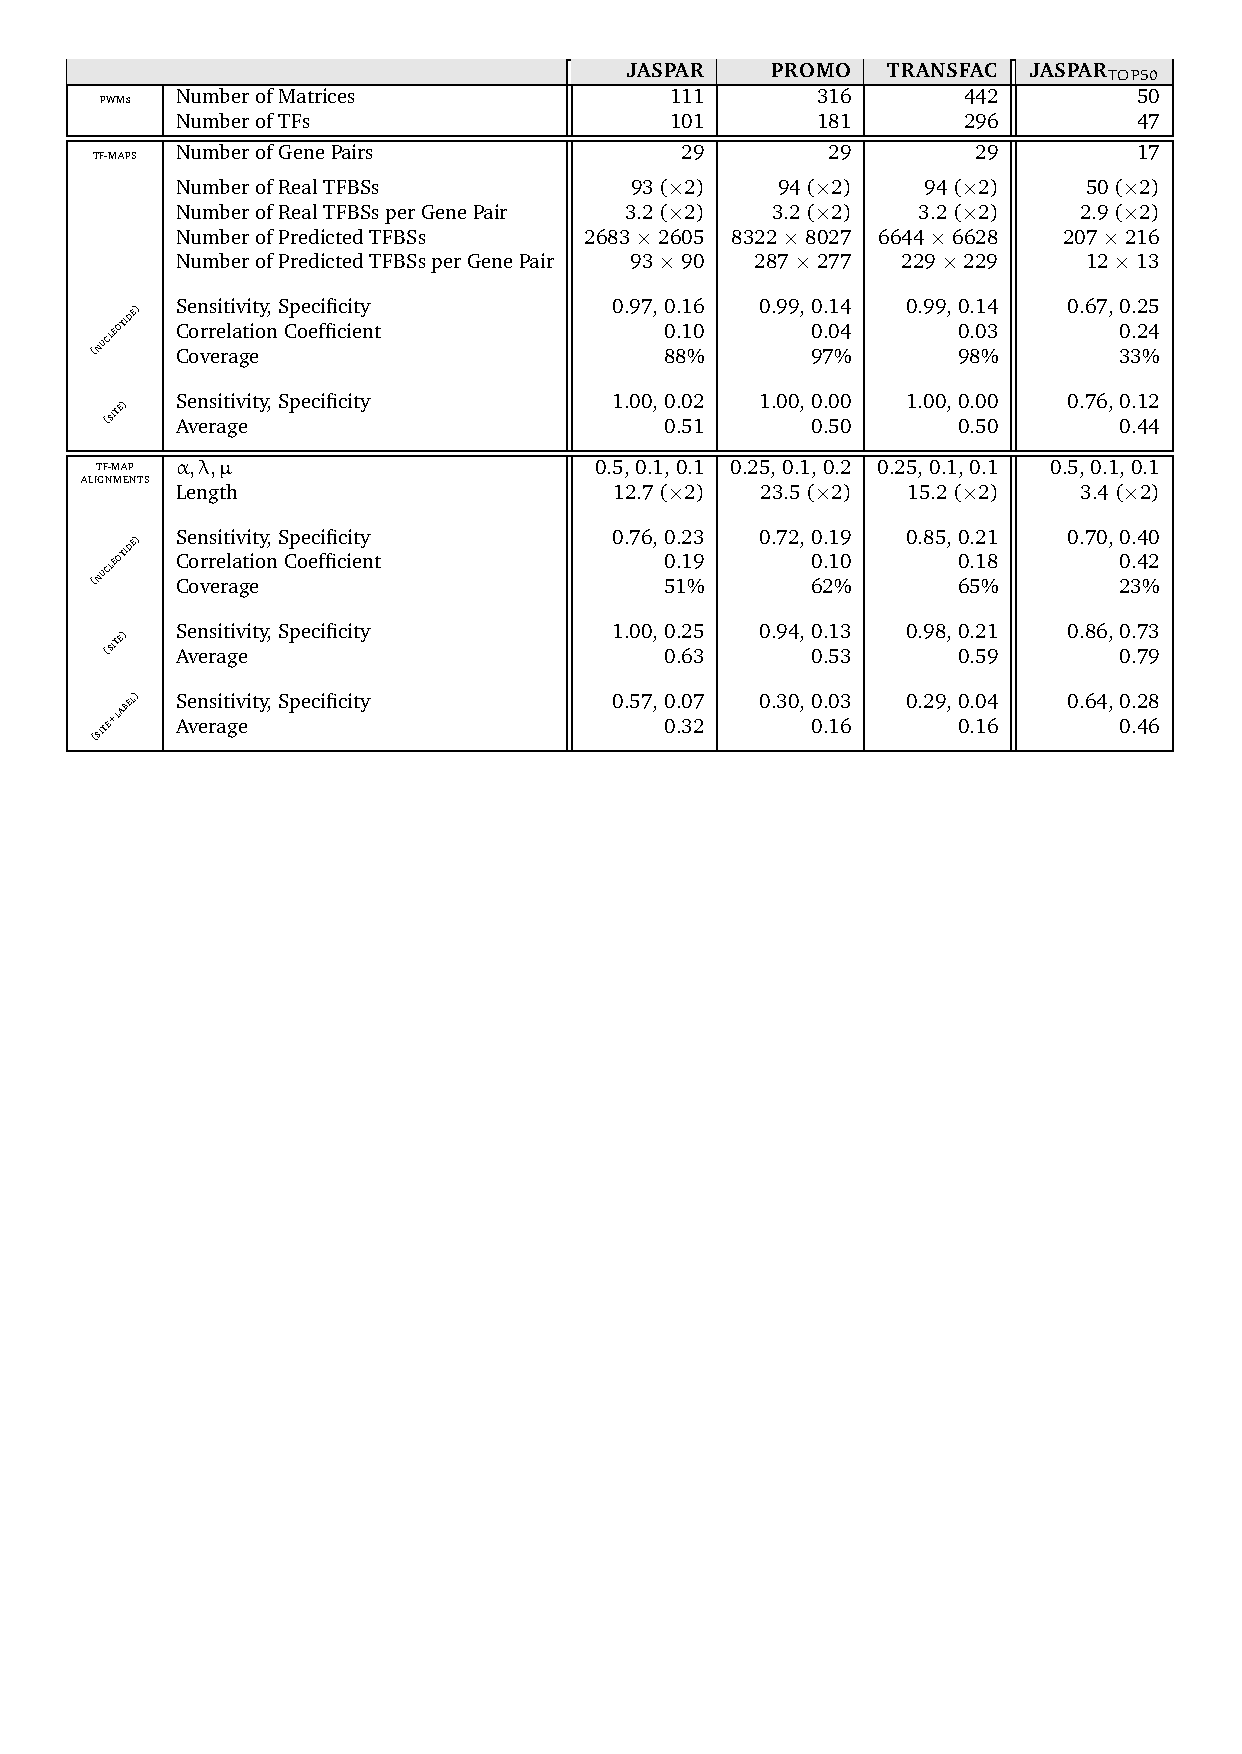
\includegraphics[bb=30 479 566 817,clip]{tables/maccuracy}
\end{center}
\end{minipage}
\mycaption{tab:accuracy}% label
          {TF-map alignment accuracy results on the \textsc{HR set}}% lof
          {TF-map alignment accuracy results on the \textsc{HR set}.}% caption header
          {\tiny Parameters were estimated independently using three
           different collections of  position weight matrices (PWMs) for
           transcription factor binding sites (TFBSs) to obtain the TF-maps of the
           promoter sequences. 
           The table has three parts. 
           On {\bf top},  number of matrices in each of these collections, and 
           the number of transcription factors (TFs) these matrices correspond to. 
           In the {\bf middle}, statistics of the resulting TF-maps: 
           number of promoter pairs (out of 36) for which matches to at least one 
           common TFBS was found in both the human and mouse orthologs 
           (and for which, therefore, there exist a non-void TF-map alignment), 
           total and average number of 
           real TFBSs per promoter sequence, total and average number of 
           predicted TFBSs per promoter sequence, and sensitivity and specificity 
           at the nucleotide and site levels (see main text for definitions). The 
           average sensitivity and specificity at the site level is the optimization 
           measure when estimating the parameters of the algorithm. Coverage is 
           the fraction of the sequence of the promoters covered by matches to TFBSs.
           At the {\bf bottom}, results of the optimal TF-alignments:
           optimal parameters and average length (number of aligned elements in the 
           optimal TF-map alignments), measures of sensitivity and specificity at the
           levels of nucleotide, site overlap, and site plus label match (see main 
           text for definitions). Coverage is the fraction of the sequence of the 
           promoters covered by matches to TFBSs.}
\end{center}
\end{table}
\end{landscape}

This number over the
total number of nucleotides in annotated TFBSs is the sensitivity, and over 
the total number of nucleotides in predicted TFBSs is the
specificity. Finally, as a summary of these two numbers we compute the
correlation coefficient. All the accuracy measures were also computed on
the initial PWM predictions, prior to the alignments.  

%%%%
% Figure 8: ABS
%%%%
\begin{figure}[t!]
\begin{center}
\setlength{\fboxsep}{0pt}
\fbox{\incgraph{width=0.85\linewidth}{ps/abs}}
\mycaption{fig:absweb}% label
          {Examples of the ABS data retrieval system}% lof
          {Examples of the ABS data retrieval system.}% caption header
          {The annotation of a gene, the set of binding motifs from a given TF in human 
           and mouse and the extraction of the promoter sequences containing such annotations
           \citep{blanco:2006a}.}% caption header.}
\end{center}
\end{figure}

\subsectionblue{Accuracy results}

\index{TF-map alignments!acc@accuracy} \index{meta-alignments!macc@accuracy} 
As it is possible to see, the main effect of the meta-alignment is the
dramatic reduction in the number of predicted TFBSs that typically
result after a PWM-based search (see also Figure \ref{fig:pspla}). Taking, for 
instance, the popular \db{Transfac} collection, the average number of TFBSs 
predicted per promoter in our dataset using this database is about 230. 
The TF-map alignment reduces this number approximately 15-fold, while 
the predicted TFBSs still covering essentially all annotated TFBSs \citep{blanco:2006b}. 
This gain in specificity is not simply due to the selection of an 
arbitrary set of non-overlapping TFBSs, since as a result of the map 
alignments the proportion of the promoter region covered by predicted 
TFBSs drops from 98\% to 65\% --a number which is more consistent with 
the estimated occupancy by TFs of the core promoter regions \citep{wray:2003a}. 

In this regard, we have compared the map alignments here with direct
sequence alignments in their ability to identify TFBSs in the promoter
regions of co-regulated genes. We have used NCBI-BLASTN \citep{altschul:1990a} 
to identify conserved blocks in the promoter region of the orthologous pairs in
the \textsc{HR set}. We have searched for local, instead of global
alignments because we expect the TFBSs to distribute discretely along
the promoter region --resulting in a patch of conserved and
non-conserved fragments. In addition, local alignments are insensible
to the relative rearrangements in the order of the TFBSs between the
promoters sequences compared. This is an advantage over the map
alignments, which require colinearity of the TFBSs in the sequences to
be compared. Despite this, and the fact that promoter elements are
usually embedded within well conserved sequences in human and mouse
orthologous promoters, map alignments are comparable or outperform the
BLASTN comparison when identifying TFBSs in them \citep{blanco:2006b}. The correlation
coefficient between the sequences covered by the BLASTN alignments and
the annotated TFBSs is $0.15$, while the same measure when considering
the sequences covered by the map alignments is $0.19$ for \db{Jaspar},
$0.10$ for \db{Promo} and $0.18$ for \db{Transfac}. Table \ref{tab:accuracy2} lists 
these values, as well as the the values of sensitivity and specificity. To obtain
these values, BLASTN was run with default parameters, but decreasing
the word size to 7 (the minimum accepted value in
NCBI-BLASTN). This allows for the detection of shorter and weaker
alignments. The performance of BLASTN degrades if we increase the word
size. We obtained similar results using the
WU-BLASTN version, which allows for shorter word sizes (data not shown).

%%%%%%%%%%%%%%%
%%% TABLE 2
%%%%%%%%%%%%%%%
\begin{table}[t!]
\begin{center}
\begin{minipage}{0.95\linewidth}\setlength{\parindent}{0pt}
\begin{center}
\scalebox{0.75}{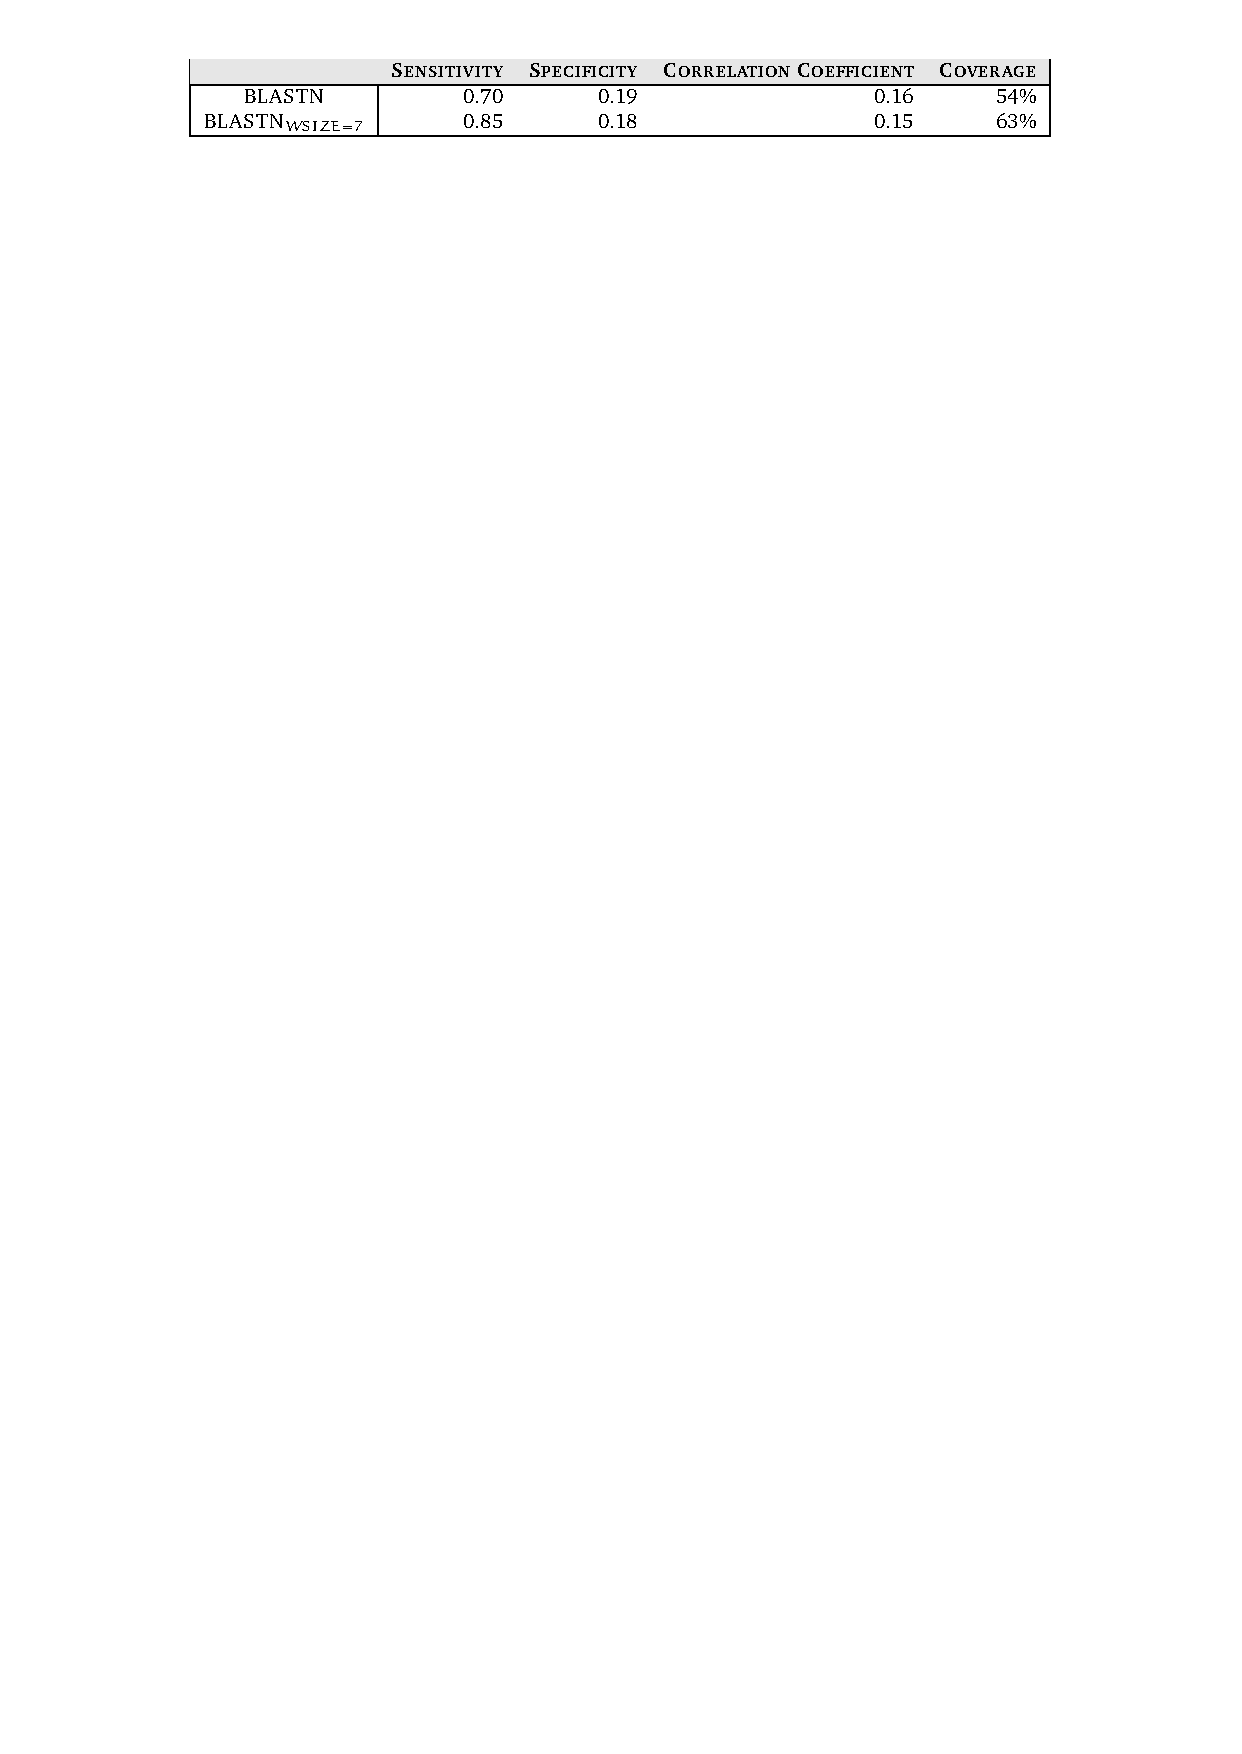
\includegraphics[bb=89 775 505 816,clip]{tables/maccuracy2}}
\end{center}
\end{minipage}
\mycaption{tab:accuracy2}% label
          {BLASTN accuracy results on the \textsc{HR set}}% lof
          {Results when using BLASTN to detect 
           conservation between orthologous pairs.}% caption header
          {}
\end{center}
\end{table}

The values in Table \ref{tab:accuracy} reflect differences between the three
collections of matrices when used in the context of the map
alignments. In this context, \db{Jaspar} appears to show the better balance
between sensitivity and specificity. This can be partially explained 
because there is less matrix redundancy --which in turn implies less
overprediction-- in \db{Jaspar} than in the other collections. To further 
minimize overprediction, we have computed the information content of 
all \db{Jaspar} matrices and selected the most informative ones. Let $P$ be 
a PWM where $P(x,i)$ denotes the probability of observing the  
nucleotide $x$ in the position $i$ of a motif of length $n$. The amount
of information $R$ of the matrix $P$ is defined as \citet{schneider:1990a}:

\begin{center}
\fcolorbox{white}{verylightgreen}{
\begin{minipage}[][][c]{0.95\linewidth}
\begin{equation}
R(P) = \sum_{i = 1 \ldots n} \left( 2 + \sum_{x\in A,C,G,T}{P(x,i) \log{P(x,i)}} \right).
\end{equation}
\end{minipage}}
\end{center}

When using the collection of the 50 \db{Jaspar} matrices with the highest $R$ value 
(which we refer to as \db{Jaspar$_{TOP50}$}) \index{JASPAR$_{TOP50}$}
to obtain the TF-maps, detection 
of TFBSs through map alignments improves over the entire set of \db{Jaspar} 
matrices: while there is some loss of sensitivity, there is a larger gain 
in specificity (see Table \ref{tab:accuracy}). 

%%%%
% Figure 9: PS-PLA1
%%%%
\begin{figure}[t!]
\begin{center}
\setlength{\fboxsep}{0pt}
\fbox{\incgraph{width=0.85\linewidth}{ps/pspla}}
\mycaption{fig:pspla}% label
          {TF-map alignment of the human and mouse PLA1A gene}% lof
          {TF-map alignment of the human and mouse PLA1A gene.}% caption header
          {Results of the TF-alignment of the human and mouse promoters of the 
           \emph{phospholipase A1 member A} gene (PLA1A, RefSeq entries NM\_015900, 
           NM\_134102). Here, the 2000 nucleotides upstream of the annotated 
           transcription start 
           site (TSS) have been considered (with position 1 corresponding to -2000). The
           TF-maps on these sequences were obtained using \db{Transfac} 6.3
           \citep{matys:2003a}. These maps contained 676 predicted binding 
           sites in human and  595 in mouse (threshold 85\%), and they are 
           represented graphically on the top right of the
           figure. Each box represents a different binding site and the color
           corresponds to the associated transcription factor (TF). The resulting
           TF-map alignment is also represented graphically at the bottom
           right. As it is possible to see, while the region 
           proximal to the TSS is not more dense in predicted TFBSs than other regions, 
           most of the aligned elements cluster near to the TSS. Indeed, more than 
           half of the elements in the TF-map alignments are within 500 nucleotides of the TSS. 
           The program GFF2PS \citep{abril:2000a} has been used to obtain the graphical 
           representation of input predictions and final alignment.}
\end{center}
\end{figure}

Finally, we have also performed a complementary
test to measure the specificity of the TF-map alignments \citep{blanco:2006b}. 
As a negative control, we have shuffled the orthologous pairing in the
\textsc{HR set} to construct a pool of unrelated human-mouse gene pairs. 
Then, the corresponding TF-map alignments between these non-orthologous paired
promoters were obtained using the parameters previously optimized.
For the three collections of matrices, the  TF-map alignments
between pairs of unrelated promoters were significantly shorter with
an average score about 50\% smaller than TF-map alignments between
``bona fide'' orthologous promoters. For instance, the average length of 
the TF-map alignments between orthologous promoters when using the \db{Jaspar} 
collection was 12.7 TFBSs, with an average score of 55.2. In contrast, 
the length of the TF-map alignments between non-related promoters was 
8.36 TFBSs, with an average score of 20.67. The sites in the
alignments involving non-orthologous gene promoters may hypothetically
correspond to general regulatory elements present in most
core promoters. An alternative, more probable, hypothesis is that they
reflect the poor specificity of most PWMs representing TFBSs.
Indeed, when we perform the same test using the more
informative \db{Jaspar}$_{TOP50}$ collection, no TF-map alignments can be 
obtained between any pair of the non-related promoters.

\sectiongreen[TF-map alignments in orthologous genes]{Using TF-map alignments to distinguish promoters from other genomic regions} 
\label{sec:testregions}

Results in the previous section indicate that alignments of TF-maps
can contribute --together with other tools, such as primary sequence
alignments-- to the characterization of the promoter region of
co-regulated genes. This contribution is mostly 
obtained through the substantial reduction of the overwhelming number 
of candidate TFBSs that PWMs and other pattern based searches 
typically produce. The co-regulated genes in the test 
case of the previous section, however, were orthologous human-mouse
pairs. The promoter regions of such pairs show substantial sequence 
conservation \citep{waterston:2002a}. It can be argued that under such 
circumstances map alignments may not be much more informative than 
primary sequence alignments. Note that, in general, good alignments 
at the primary sequence level will inevitably result 
--given the low specificity of the PWM search-- in good 
map alignments, although such map alignments may bear 
little relationship to the underlying conserved 
configurations of TFBSs. To assess to what extent good 
TF-map alignments are simply a reflection of underlying 
sequence conservation, we have compared the meta-alignments obtained using 
\db{Jaspar}$_{TOP50}$, in the 200 nucleotides of the promoter region of the 36 
gene pairs from the \textsc{HR set}, with the meta-alignments obtained in fragments 
of 200 nucleotides from intergenic (2000 nucleotides upstream of the TSS), 
5'UTR (downstream of the TSS), coding (downstream of the translation start 
site and considering only coding DNA), intronic (downstream of the first intron 
junction), and downstream (downstream of the transcription termination 
site) sequences. The test is graphically represented In Figure 
\ref{fig:testregions}.

We have computed the average score of the map alignments in each of the genomic 
regions and have identified, for each homologous pair, the genome regions in which 
the alignment produces the highest score \citep{blanco:2006b}. We have performed 
the same exercise using global pairwise sequence alignments, obtained with CLUSTALW 
\citep{thompson:1994a}. 
Results appear in Table \ref{tab:testregions} (Top). As expected, nucleotide sequence
alignments score the highest in the coding regions (in 26 out of 36
cases), followed by the alignments in the promoter (5 out of 36) and
5$^\prime$ UTR regions (4 out of 36). The scores of the sequence 
alignments show that promoter regions are less conserved than coding regions,
and have a level of conservation similar to that observed in 5'UTRs. 
Despite this, TF-map alignments score the highest in the promoter
regions (in 25 out of 36), where the average score of map alignments 
is almost twice as high as that of the coding regions. Only in 6 out
of 36 cases the TF-map alignment scores the highest in coding regions. 
Interestingly, while intron sequences in the orthologous human-mouse
pairs are much less conserved than 5'UTRs, TF-map alignments 
have a similar score in both regions. In fact, in 3 cases, TF-map
alignments have the highest score in first introns, while only in 1 case in
5'UTRs. This is consistent with the fact that first introns are known
to often contain regulatory motifs. 

%%%%
% Figure 10: TestRegions
%%%%
\begin{figure}[t!]
\begin{center}
\setlength{\fboxsep}{0pt}
\fbox{\incgraph{width=0.75\linewidth}{ps/testregionsS}}
\mycaption{fig:testregions}% label
          {TF-map alignment on several genomic samples}% lof
          {TF-map alignment on several genomic samples of two species.}% caption header
          {}
\end{center}
\end{figure}

In order to measure the ability of TF-map alignments
to detect conserved regulatory elements at larger
evolutionary distances --at which the degree of sequence
conservation may be negligible-- we have carried out the same analysis
on a set of human-chicken orthologous pairs derived from the \textsc{HR
set}.  Using the RefSeq gene set as mapped into the UCSC genome browser,
we have identified the chicken ortholog for 25 genes in the
\textsc{HR set}. We refer to the resulting set of human-chicken gene pairs as the
\textsc{HC set} \citep{blanco:2006b}. As before, we have compared
promoter, intergenic, 5'UTR, coding, intronic and downstream sequences
between the orthologous human-chicken genes using both TF-map
alignments based on \db{Jaspar}$_{TOP50}$ and sequence alignments using CLUSTALW.
Results appear in Table \ref{tab:testregions} (Bottom). 
While, as expected, the scores of the alignments are, in both cases, clearly
lower for human--chicken than for human--mouse comparisons,
the same relative trends can be observed, with sequence alignments
being most significant between coding regions, and TF-map alignments
between promoter regions.
However, while coding sequences are still distinctively conserved
between human and chicken, similarity in promoter sequences degrades
substantially.  
Indeed, in contrast with human-rodent comparisons,  5'UTRs are, for
instance clearly more conserved than the promoters between human and chicken
orthologous genes. Despite this lack of sequence similarity in the
human-chicken promoter pairs and the fact that we trained our
algorithm specifically on human and rodent genes, 
the TF-maps remarkably still score the highest in these regions (in 9 out of 25).
Interestingly, TF-map alignments are able to score comparatively high 
in downstream regions even though they do not appear to exhibit
sequence conservation; regulatory
motifs have been occasionally reported on these regions.
Overall, these results indicate that alignments of TF-maps are able to detect
conservation of regulatory signals, which can not be detected by
sequence similarity alone \citep{blanco:2006b}.

%%%%%%%%%%%%%%%
%%% TABLE 3
%%%%%%%%%%%%%%%
\begin{table}[t!]
\begin{center}
\begin{minipage}{0.98\linewidth}\setlength{\parindent}{0pt}
\begin{center}
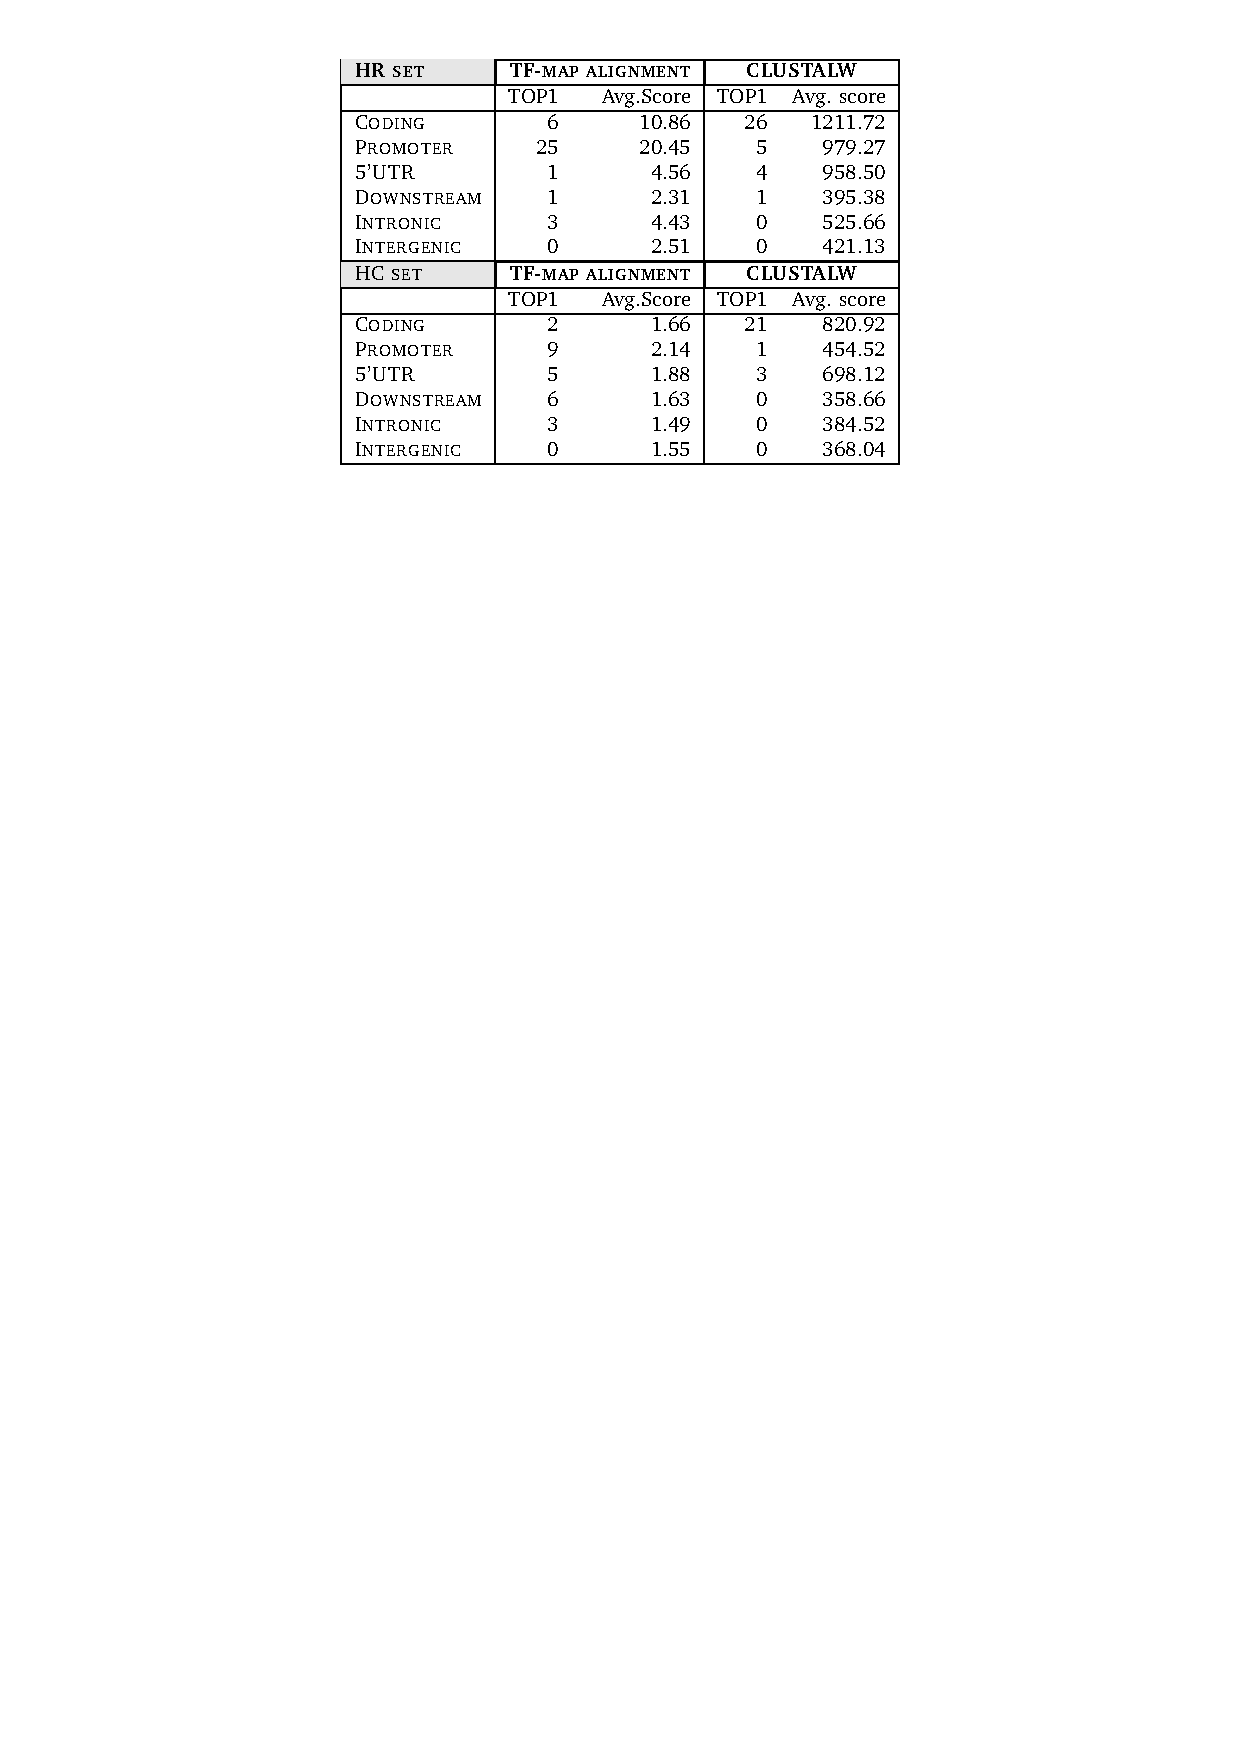
\includegraphics[bb=161 608 434 816,clip]{tables/testregions}
\end{center}
\end{minipage}
\mycaption{tab:testregions}% label
          {TF-map alignment results on several genomic samples.}% lof
          {TF-map alignment results on several orthologous genomic samples}% caption header
          {(Top) Sequence and TF-map alignments of different genomic regions
           between the human and mouse orthologous pairs in the \textsc{HR set}. 
           (Bottom) Sequence and TF-map alignments of different genomic regions
           between the human and chicken orthologous pairs in the \textsc{HC set}.
           TOP1 is the number of pairs in which the highest scoring alignment is found 
           in a given genomic region.}
\end{center}
\end{table}

\subsectionblue{Promoter identification with TF-map alignments}

\index{TF-map alignments!prom@promoter identification} \index{promoter!idtf@identification} 
Promoter identification is still a difficult problem (reviewed in Chapter 
\ref{sec:genefinding}). TF-map alignments may be helpful in this problem. Using a set
of $278$ orthologous human-chicken gene pairs of another study \citep{abril:2005a},
we have performed the following experiment.

We have extracted the human promoter of these genes ($500$ nucleotides) from the 
UCSC human genome distribution according to the RefSeq coordinates. For the chicken 
genes, we have extracted the mRNA from the chicken genome surrounded by $5,000$ 
nucleotides upstream of the TSS and $5,000$ downstream of the end of the transcript. 
Finally, we have extracted samples of $500$ nucleotides from these long sequences,
without overlapping between each contiguous windows. For each gene, the upstream promoter 
region, orthologous to that of human, is therefore located in the window between the 
positions $4,500$ and $5,000$ nucleotides (see Figure \ref{fig:testpromoterpgws}).

Next, we have used the $50$ more informative matrices from \db{Transfac} \citep{matys:2003a} 
as a mapping function to obtain the
map of each sample in the chicken sequences. We have also used \db{Transfac} for mapping
the predicted TFBSs on the human promoters. The experiment consisted in
performing the pairwise TF-map alignment between the human promoter and all of the
samples in its chicken ortholog. Then, for each window we have counted in how many
cases out of the $278$ genes the TF-map alignment between the human promoter and that 
window sample scores the highest, among all of the windows. As shown in Table 
\ref{tab:testpromoter}, the chicken gene fragment in which more genes hit the best 
was the $4,500-5,000$ sample (31\%), which corresponds with the upstream promoter region 
according to the RefSeq annotations. In addition, 14\% and 21\% of the 278 gene pairs 
obtained the highest TF-map alignment score on the windows located at $4,000-4,500$ and 
$5,000-5,500$, respectively. This bias is not observed in the rest of the windows.
These percentages agree well with the errors in the precise TSS annotation \citep{suzuki:2004a}.

We also counted for each window in how many cases the meta-alignment between this
sample and the human orthologous promoter scores among the TOP-10 best alignments.
Despite the results are less significant, it is interesting to notice that in more
than 200 gene pairs (76\%), the TF-map alignment between the human promoter and
the chicken sample in the window $4,500-5,000$ was among the TOP-10.
We repeated the test with the full collection of \db{Transfac} 6.3 ($442$ matrices). The
results, shown in Table \ref{tab:testpromoter}, are slightly worse. This fact is
probably related to the poor specificity of many matrices that are included in the full 
collection.

Again, we performed the same experiment with the program BLASTN, using the score of the 
best HSP on each alignment to rank the window comparisons. Table \ref{tab:testpromoter} 
lists the results. The sequence alignments can detect correctly the actual promoter 
pair in less than 16\% of the $278$ genes (31\% among the best 10 alignments).

Future experiments should be conducted in a genome-wide mode to verify the accuracy
of TF-map alignments in larger datasets. However, the meta-alignment, at least in this 
set of $278$ gene pairs, was clearly superior to sequence alignment to detect the correct
promoter region. In principle, we could be able with the TF-map alignments 
to accurately detect the promoter region in one species, scanning this genome with the 
orthologous promoter in the other informant genome.

%%%%
% Figure 11: testPromoterRegion
%%%%
\begin{figure}[t!]
\begin{center}
\setlength{\fboxsep}{0pt}
\fbox{\incgraph{width=0.75\linewidth}{ps/testpromoter}}
\mycaption{fig:testpromoterpgws}% label
          {TF-map alignment in promoter detection}% lof
          {TF-map alignment in promoter detection.}% caption header
          {}
\end{center}
\end{figure}

\subsubsectionblue{Parallel meta-alignment: PGWS}
\index{meta-alignments!pgws@parallel} \index{PGWS}
Let $M$ be a long genomic region of $m$ nucleotides. Let $P$ be a short genomic 
sequence of $p$ nucleotides, with $m >> p$. The problem of mapping and aligning 
the sequence $P$ to a contiguous set of windows in $M$ must be carefully analyzed
to obtain in a reasonable  amount of time that window from $M$ whose TF-map alignment 
to $P$ reaches the highest value. If $p=500$ bps, $m=20,000$ bps and the windows are 
$500$ bps with an overlap between adjacent windows of $100$ bps then the number of 
windows (that matches the number of pairwise TF-map alignments to do) is 50. Obviously, 
if the test is repeated for hundreds of gene pairs, the computation of the best windows 
requires some improvement.

In fact, the calculation of the TF-map alignment between $P$ and a given window from
$M$ is independent from the rest of alignments. Thus, the alignments can be easily
dispatched to different processors to be performed in parallel. At the end of the
process, the scores of the alignments are ranked and displayed. Notice we are only 
interested in the score of the alignments to construct a ranking so the TFBSs that 
actually constitute them are logically not necessary in this case. Thus, we
register the value calculated on each dynamic programming similarity matrix,
but the paths of the alignments are not constructed.

Following with the same example: if there are $10$ available processors, we can divide
uniformly the list of windows (alignments) among them using any offset schema to
ensure the load of each processor is similar. For instance, if we consider an
offset of $4,000$ bps between two windows that are processed by the same unit,
we will assign the series of alignments 
$(M_{0-500},M_{4000-4500},M_{8000-8500},M_{12000-12500},M_{16000-16500}$
to the processor $P_1$, the series 
$(M_{400-900},M_{4400-4900},M_{8400-8900},M_{12400-12900},M_{16400-16900}$
to the processor $P_2$ and so on. The chronograph of events associated to
this parallel processing is:

\begin{center}
\setlength{\fboxsep}{0pt}
\incgraph{width=0.75\linewidth}{ps/chronogram}
\end{center}

In this case, we can divide the sequential time $T(n)$ by the number of
processors so that the parallel time is $\frac{T(n)}{10}$. We can then
compute $50$ TF-map alignments with $10$ computers using the same amount
of time that is necessary for calculating $5$ alignments in a single processor
machine. As the same comparisons must be done for hundreds of genes, the
save of time using this parallel version is considerable. 

The program \prog{pgws} (Promoter Genome-Wide Search) is a generalization of
the schema presented here, in which the input consists of a list of probes
$P=p_1,p_2 \ldots p_{|P|}$ (gene promoters from species $A$) and a list of long
genomic sequences $M=m_1,m_2 \ldots m_{|M|}$ (chromosomes from species $B$).
In an efficient parallel environment, the program \prog{pgws} may be used, for 
instance, to locate the ortholog promoter of a chicken gene in the human genome.


\sectiongreen[TF-map alignments in co-regulated genes]{Using TF-map alignments to characterize promoter regions of 
co-regulated genes}\label{sec:cisred}

\index{TF-map alignments!cisred@in CISRED} \index{meta-alignments!mcisred@in CISRED} 
We expect, therefore, the map alignments to be particularly useful to
characterize promoter regions of co-regulated genes in absence of
sequence conservation. In such cases, the map alignments can help to
recover conserved configurations of TFBSs that primary sequence
comparisons would not. It is important to stress in this regard, that
the match state in the alignment of TF-maps is defined based on the
transcription factor label, and not based on the label of the specific
binding site. Since a given TF can be associated to
different binding sites (for instance, the approximately 90 TFBSs in
the \textsc{HR set} correspond only to about 30 TFs), an alignment of TF-maps
can include the alignment of TFBSs that show no sequence conservation.

%%%%%%%%%%%%%%%
%%% TABLE 4
%%%%%%%%%%%%%%%
\begin{table}[t!]
\begin{center}
\begin{minipage}{0.98\linewidth}\setlength{\parindent}{0pt}
\begin{center}
\scalebox{0.8}{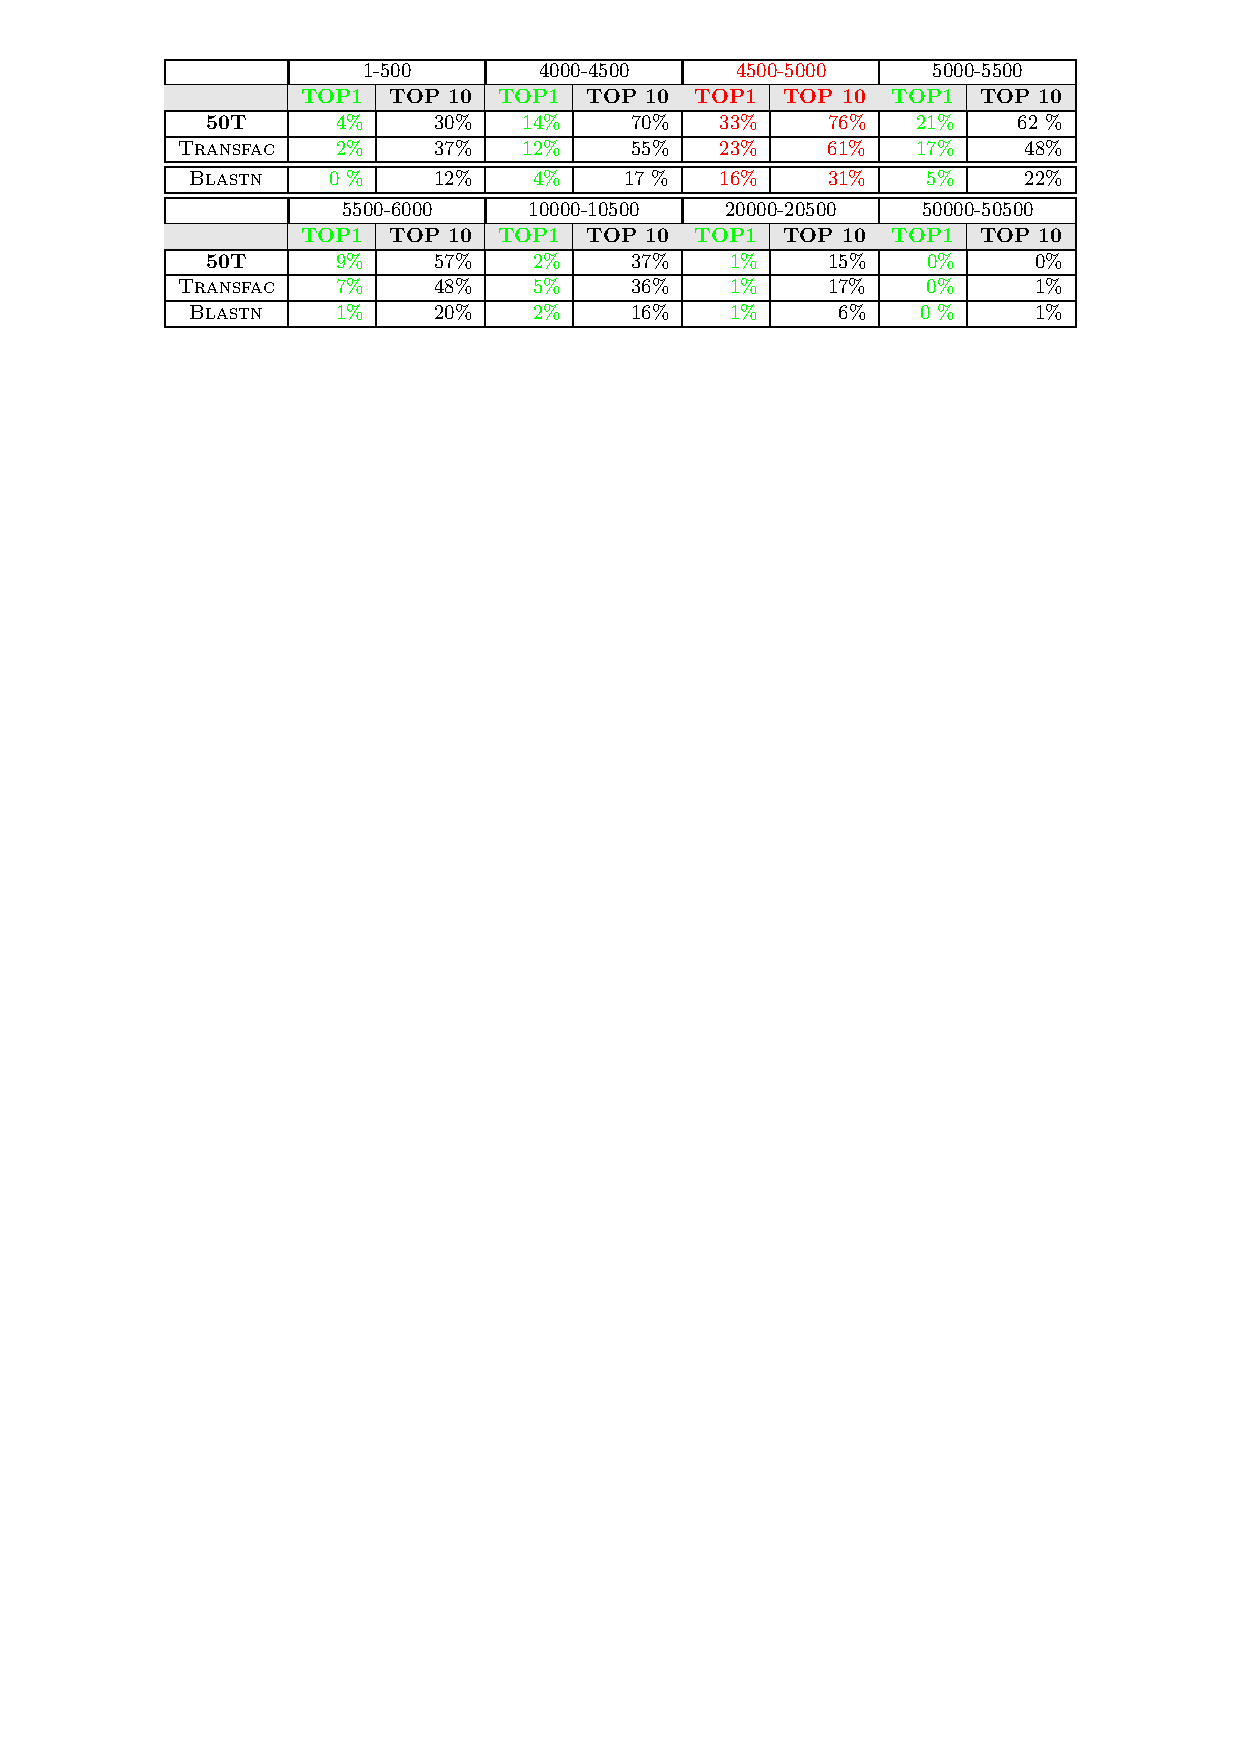
\includegraphics[bb=75 681 519 817,clip]{tables/testpromoter}}
\end{center}
\end{minipage}
\mycaption{tab:testpromoter}% label
          {Promoter identification with human-chicken TF-map alignments}% lof
          {Promoter identification with human-chicken TF-map alignments.}% caption header
          {The percentages are relative to the proportion of the $278$ human-chicken promoter
           pairs that score the highest in each window (or within the TOP 10). The correct 
           promoter window is $4,500-5,000$. The $50$T collection are the $50$ more informative 
           matrices from \db{Transfac}.}
\end{center}
\end{table}

Many examples could be found in which map alignments produce a better
characterization of the promoter region of co-regulated genes than
that obtained through primary sequence alignments. We would like,
however, to move beyond such an anecdotal evidence, and have a more
exhaustive evaluation of the power of TF-map alignments to characterize
promoter regions of co-regulated genes in absence of sequence
similarity. Towards such a goal we have used the set of co-regulated
genes in the CISRED database \citep{robertson:2006a}. The CISRED \index{CISRED}
database is primarily a collection of conserved regulatory sequence
elements identified by a genome-scale computational system that uses
pattern discovery, similarity, clustering, co-occurrence and co-expression 
calculations. CISRED includes, as well, a database of high-confidence 
co-expressed gene pairs \citep{griffith:2005a}, obtained from cDNA microarray 
hybridization, SAGE and other experiments, as well as Gene Ontology 
(GO, \cite{tgoc:2000a}) analysis. Version 1 of CISRED high confidence 
co-expression human set contains 60,912 co-expression gene pairs for 5562 genes. 
Because of the criteria to establish co-regulation within CISRED, we do not 
expect strong bias towards co-expression pairs sharing strong sequence 
similarity in their promoter regions. 

We have, thus,  performed the following experiment (graphically represented
in Figure \ref{fig:cisred}):
we have compared the promoter region of each gene $x$ in the CISRED
set with the promoter regions of the genes co-regulated with $x$,
$coreg(x)$, and with the promoter region of the genes no co-regulated
with $x$, $\overline{coreg}(x)$. Even though the promoter of the gene
$x$ may not show stronger sequence similarity with the promoters of the
genes in $coreg(x)$ than with the promoters of the genes in 
$\overline{coreg}(x)$, our assumption is that it will still share
some common regulatory signal (maybe very weak) with the promoters of
the (at least a fraction of) the genes in $coreg(x)$, whereas no
common signal will be shared between the promoter of $x$ and the
promoters of the genes in $\overline{coreg}(x)$. Our hypothesis is
therefore that alignments of TF-maps will be superior in detecting
such signals to alignments of the primary nucleotide sequence. 

We have proceed in the following way:
we have used ENSMART to extract 500 nucleotides
upstream of each gene in CISRED according to genome coordinates in 
\ensembl{}. We have used 500 nucleotides upstream here, instead of 
200 nucleotides as before, because of the intrinsic imprecision 
of \ensembl{} when annotating the coordinates of the TSS.  
We obtained such a sequence for 5333 out of 5562 CISRED genes
and considered it the promoter region of the gene. For this set of 
5333 genes, 56,632 co-expression gene pairs are described in CISRED.
We have used next the collection
of matrices in \db{Jaspar}$_{TOP50}$ (see previous section) to obtain the
TF-maps of each promoter region. Then for each gene
$x$ we have obtained the optimal map alignment with each gene in
$coreg(x)$ and in $\overline{coreg}(x)$. We have used the enhanced 
TF-map alignment algorithm
with the optimal parameters estimated in the training procedure. 
Finally, we have determined whether
the scores of the map alignments between the promoter of gene $x$ and
the promoters of the genes in $coreg(x)$ were significantly higher
than the scores of the map alignments between the promoter of gene $x$
and the promoters of the genes in $\overline{coreg}(x)$. Because the
scores of the optimal TF-maps alignments follow, as optimal sequence
\index{TF-map alignments!dis@score distribution} \index{meta-alignments!mdis@score distribution} 
alignments, a Gumbel or extreme-value distribution (see Figure \ref{fig:gumbel}), 
we calculated the Wilcoxon test to assess this
hypothesis. We obtained 42,756 non-void $coreg(x)$ alignments and 
20,600,640 non-void $\overline{coreg}(x)$ alignments. 
4,784 genes in CISRED had non-void alignments for both the 
$coreg(x)$ and the $\overline{coreg}(x)$ sets . The
average score of the $coreg(x)$ alignments was 6.02, and the average
length 2.13 sites. For the $\overline{coreg}(x)$ alignments, the values were
5.57 and 2.06, respectively. For 97 genes,
the score of the $coreg(x)$ alignments was significantly
higher than that of the $\overline{coreg}(x)$ alignments at a
significance level of p=0.01. At a p-value of 0.001, the number was 23. 
Since CISRED is partially based on microarray
experiments, one could argue that cross-hybridization with recently
duplicated genes may artefactually bias these results. However, no 
duplicated copies of genes exist in the sets of co-regulated genes with 
the 97 positive cases above.

%%%%
% Figure 12: the CISRED experiment
%%%%
\begin{figure}[t!]
\begin{center}
\setlength{\fboxsep}{0pt}
\fbox{\incgraph{width=0.75\linewidth}{ps/cisred}}
\mycaption{fig:cisred}% label
          {Alignment experiment with the CISRED genes}% lof
          {Alignment experiment with the CISRED genes.}% caption header
          {}
\end{center}
\end{figure}

We performed the same experiment, using BLASTN \citep{altschul:1990a} 
instead to compare the promoter region of each gene $x$ in the CISRED set 
with the promoters of the genes in $coreg(x)$ and $\overline{coreg}(x)$. 
BLASTN was used with the parameters word size 7 and expectation value 10 
so that short stretches of conservation could also be retrieved. In each 
comparison, we identified the score of the best HSP. We obtained 981 $coreg(x)$
alignments and 445,371 non-void $\overline{coreg}(x)$ alignments.
653 genes in CISRED had BLASTN alignments in both the 
$coreg(x)$ and the $\overline{coreg}(x)$ sets. The
average score of the $coreg(x)$ alignments was 29.9, and the average
length 51 nucleotides. For the $\overline{coreg}(x)$ alignments, the values 
were 24.3 and 40.5, respectively. For 11 genes,
the score of the $coreg(x)$ alignments was significantly
higher than that of the $\overline{coreg}(x)$ alignments at a
significance level of p=0.01;  there was
only one gene for which the score of the $coreg(x)$ alignments was 
significantly higher than that of the $\overline{coreg}(x)$ alignments,
at a significance level of p=0.001. 

We have investigated whether differences in conservation of regulatory
elements could be found between promoters associated to CpG islands
(CpG+) and promoters not associated to them (CpG-). CpG- promoters
have been linked to tissue-specific expression patterns 
\citep{smale:2003a}, and therefore they could be
overrepresented in the set of co-expressed genes for which we have
been able to identify conserved regulatory motifs. 
We computed for each gene the GC content and the CpG score as defined by
\citet{yamashita:2005a}. The presence of a CpG island on a window (-100:+100)
centered around the TSS of a gene is accepted when its GC content is
greater than 0.5 and when its CpG score is greater than 0.6 (CpG+); 
otherwise they are classified as CpG
negative genes (CpG-). Genes lacking CpG islands around their TSS have been
shown to have a more tissue-specific expression pattern
\citep{yamashita:2005a}. 
Based on these considerations, 3844 out of the 5333 promoters (72\%)
were identified as CpG+ genes, while only 1489 (28\%) were classified as
CpG-. Among the 97 genes for which  
the score of the $coreg(x)$ TF-map alignments was significantly
higher than that of the $\overline{coreg}(x)$ alignments at a
significance level of p=0.01, 63 were CpG+ (65\%). At a p-value of
0.001, the number of CpG+ genes was 13, out of a total of 23 (56\%).
It, thus, indeed appears that genes with CpG- promoters are slightly
overrepresented in the set of co-regulated genes with conserved
(specific) regulatory signals.

%%%%
% Figure 13: gumbel distributions
%%%%
\begin{figure}[t!]
\begin{center}
\setlength{\fboxsep}{0pt}
\begin{tabular}{|cc|}
\hline
\incgraph{width=0.35\linewidth,height=8cm}{ps/gumbel1} &
\incgraph{width=0.35\linewidth,height=8cm}{ps/gumbel2}\\
\hline
\end{tabular}
\mycaption{fig:gumbel}% label
          {Score distribution of the CISRED TF-map alignments}% lof
          {Score distribution of the CISRED TF-map alignments.}% caption header
          {(Left) Distribution of the $coreg(x)$ TF-map alignment scores. 
           (Right) Distribution of the $\overline{coreg}(x)$ TF-map alignment scores.}
\end{center}
\end{figure}


As it is possible to see, despite the general poor ability of both the
sequence alignments and the TF-maps to uncover relationships between
the promoters of the co-regulated genes in CISRED, it is clear that
TF-map alignments are able to detect more relationships than
BLASTN alignments (97 vs. 11 at a  p-value $<$ 0.01, 23 vs. 1 at a
p-value $<$ 0.001). It can be argued that this is partially an artefact,
resulting from BLASTN reporting only sequence alignments over a given
threshold, while non void TF-map alignments are always produced, provided that
the maps to align share at least one common element. 
In fact, given the number of genes for which valid alignments are
obtained, at a p-value $<$ 0.01 there are twice as many cases in 
which $coreg(x)$ scores are significantly higher than $\overline{coreg}(x)$ as 
expected if there was actually no difference in the distributions of scores, both using 
TF-map and sequence alignments.
At a p-value $<$ 0.001, however, the number of cases in which $coreg(x)$ scores
are significantly higher than $\overline{coreg}(x)$ coincides with the expected 
value using BLASTN, but it is five times the expected value, using TF-maps. 
We believe that this indicates that, even after taking into account the
effect of the different number of total alignments reported, 
the TF-map alignment algorithm is superior to BLASTN in
detecting relationships between the promoter regions of co-regulated
genes. Indeed, among the 445,371 total BLASTN alignments obtained,
there are 981 alignments between co-regulated genes, while 
the 445,371 top scoring TF-map alignments obtained include 1240
alignments between co-regulated genes.
Interestingly, there are only 148 alignments in common
between both approaches, indicating that they could be used to
complement each other.

%%%%%%%%%%%%%%%
%%% TABLE 5
%%%%%%%%%%%%%%%
\begin{table}[t!]
\begin{center}
\begin{minipage}{0.98\linewidth}\setlength{\parindent}{0pt}
\begin{center}
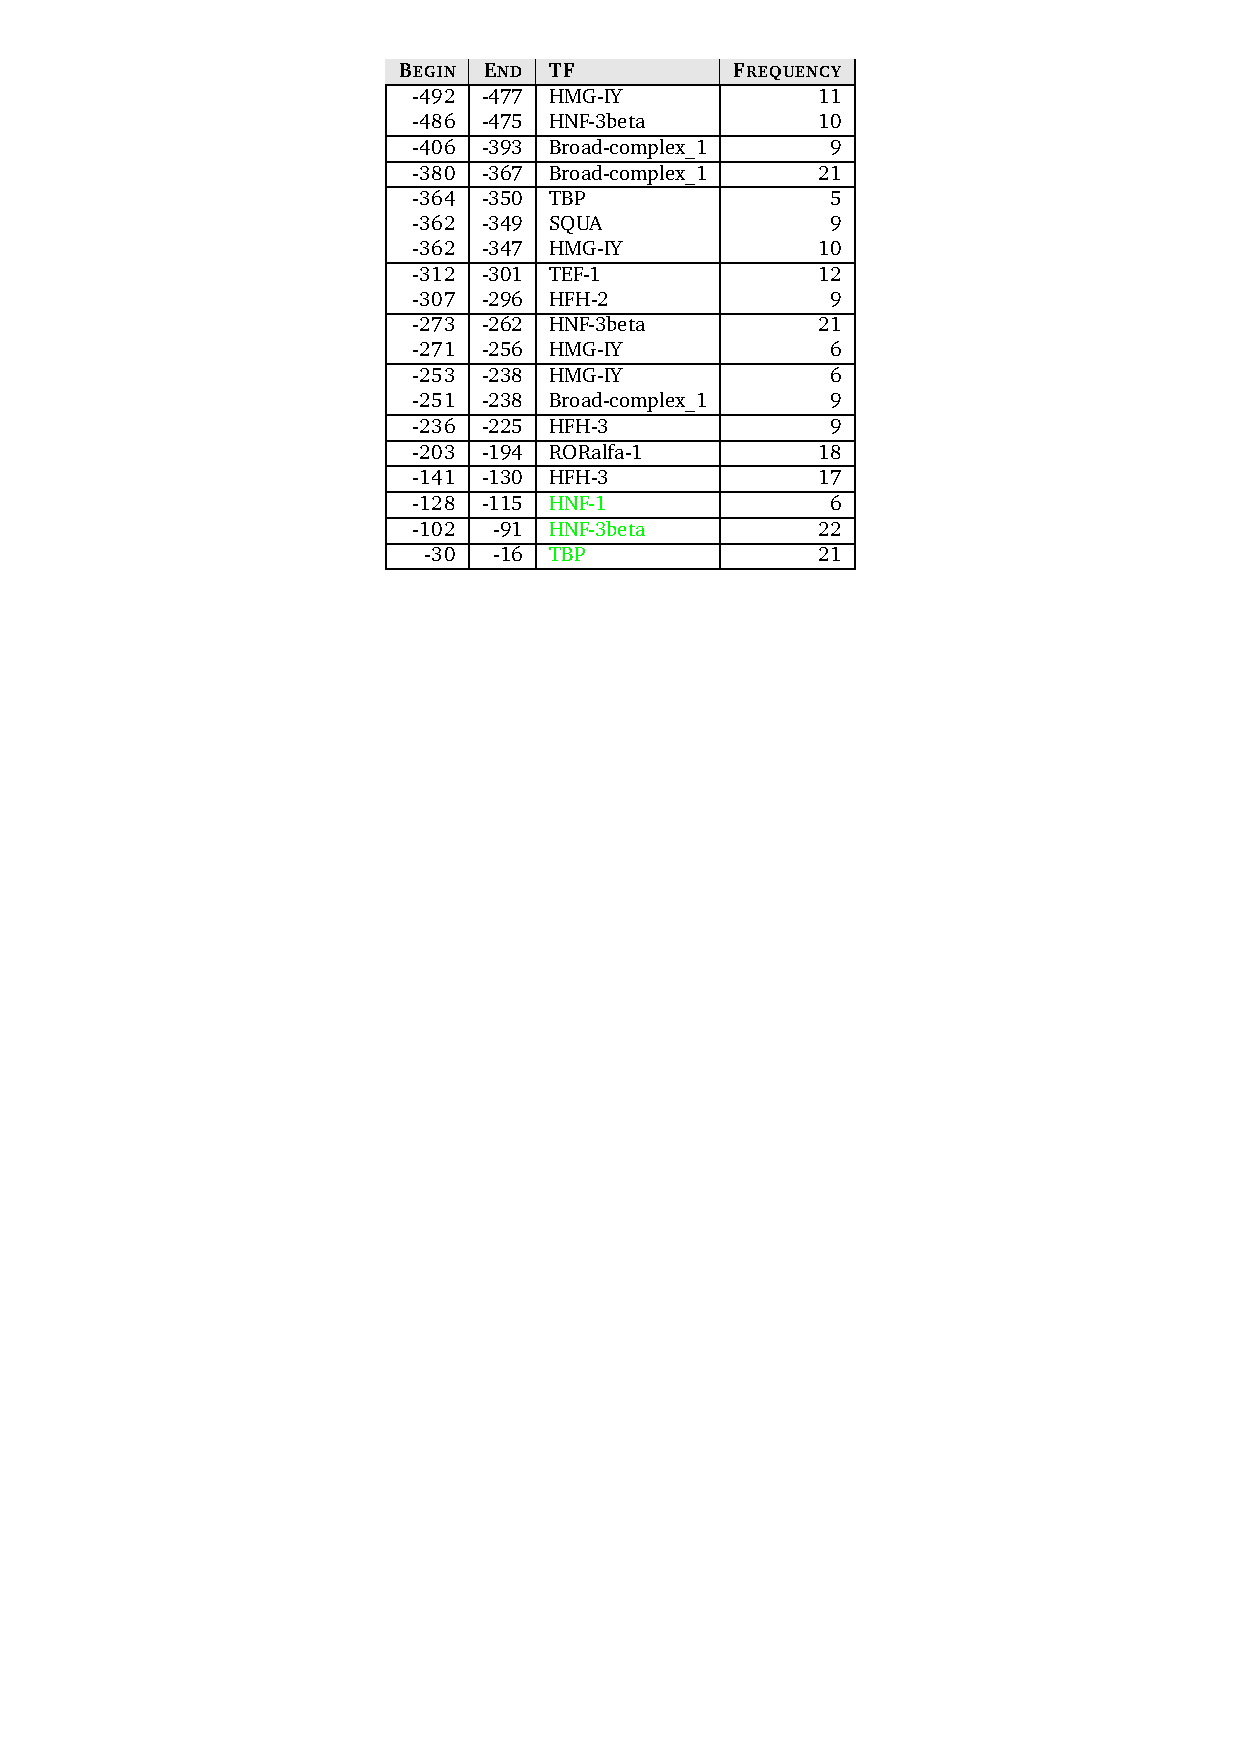
\includegraphics[bb=181 566 414 817,clip]{tables/ttr}
\end{center}
\end{minipage}
\mycaption{tab:ttr}% label
          {Reconstruction of the TTR gene promoter}% lof
          {TF-map alignment reconstruction of the TTR gene promoter.}% caption header
          {Summary of the TF-map alignments obtained between the
promoter of the \emph{transthyretin} gene (TTR, \ensembl{} entry ENSG00000118271)
and the promoters of the genes co-regulated with it according to the CISRED 
database. The table lists the predicted transcription factors on the promoter 
of \emph{transthyretin}, which appear at least in five TF-map alignments with
co-regulated genes. The experimentally verified sites are highlighted.}
\end{center}
\end{table}

It could be argued that the superiority of the TF-map over sequence
alignments has little to do with the alignments and more to do with the
maps. In other words, we would have obtained similar results if we
were to simply score the proportion of TF labels common to the
compared promoter regions --without the need for an
alignment. Therefore, we have computed such a score for each pair of
genes in CISRED: if $p$ and $q$ are the sets of elements in the 
TF-maps of the promoters to be compared, we have computed  
${|p \cap q|^2} / {|p| \cdot |q|}$, where $|p|$ is the size
(cardinality) of the set $p$. Among the 445,371 top scoring
comparisons, 1072 corresponded to co-regulated genes
(with only 394 gene comparisons in common with the TF-map alignment approach), 
a value intermediate between that obtained with sequence and with TF-map
alignments. This reflects that conservation of the relative position of
the TFs along the primary sequence, and not only
common presence, is indicative of gene co-regulation. Conservation of
relative position can only be captured by TF-map alignments.

As an example, Table \ref{tab:ttr} summarizes the TF-map alignments
obtained when aligning the promoter region of the \emph{transthyretin}
gene (TTR, \ensembl{} entry ENSG00000118271) with that of its
co-regulated genes in CISRED. TTR is a serum carrier protein expressed
in liver and brain. The regulatory regions that control the TTR
expression in liver have been experimentally determined \citep{costa:1989a}, 
and consist of a 100-nucleotide enhancer located at -2000 nucleotides 
upstream of the TSS and
a proximal promoter region between -200 and -90 nucleotides upstream of the TSS
(relative to the coordinates in the \ensembl{} entry).
This proximal region is constituted of 6 binding
sites (coordinates relative to TSS of the \emph{transthyretin} 
gene as in the \ensembl{} database): HNF-1 (-137,-109),
HNF-3 (-140,-128 and -106,-91), HNF-4 (-151,-140), C/EBP binding
(-195,-177 and -135,-112). The TATA box is located at -30.
CISRED lists 105 genes co-regulated with TTR. Interestingly, while
BLASTN is unable to detect any sequence 
similarity between the promoter of TTR and that of its co-regulated
genes,  TF-map alignments are obtained in 83
cases, and scored significantly (p-value $<$ 0.001). We have 
reconstructed the structure of the TTR promoter from
the elements that appear in the TF-map alignments. 
A total of 35 TFBSs were initially mapped with \db{Jaspar}$_{TOP50}$ in the 
TTR promoter. For each predicted TF, Table \ref{tab:ttr} lists the number of 
TF-map alignments between TTR, and its co-regulated genes in which the TF appears. 
Only elements appearing in at least five alignments are reported. No matrices 
for the detection of C/EBP and HNF-4 were included in the \db{Jaspar}$_{TOP50}$ collection 
that was used to perform the test. However, the meta-alignments were 
overrepresented in the other experimentally annotated sites, HNF-1, HNF-3 and TATA,
exactly in the region were promoter activity has been reported
(see Figure \ref{fig:ttrannot}). The binding of HNF-3 to positions -140,-128 
is not directly reported. The
TF-map alignments, however, are highly enriched in the HFH-3 factor 
(HNF3/fork head homolog) at this region. In fact, both share a similar 
consensus binding sequence in \db{Transfac} \citep{matys:2003a}: TRTTTRTTT for 
HFH-3 and TRTTTRYTT for HNF-3. 

%%%%
% Figure 14: TTR promoter
%%%%
\begin{figure}[t!]
\begin{center}
\setlength{\fboxsep}{0pt}
\fbox{\incgraph{width=0.75\linewidth}{ps/ttr}}
\mycaption{fig:ttrannot}% label
          {Experimental annotation of the TTR gene}% lof
          {Experimental annotation of the TTR gene promoter.}% caption header
          {Binding sites for activators that control transcription of the mouse 
           \emph{transthyretin} (TTR) promoter in hepatocytes are shown. Adapted from \citep{lodish:2000a}.}
\end{center}
\end{figure}

\subsubsectionblue{Fast computing of all the CISRED TF-map alignments}

For the results of this section, it was necessary to perform 
$5,333 \times 5,333 = 28,440,889$ pairwise TF-map alignments. These combinations 
can be represented into a similarity matrix that is addressed by 
the $5333 \times 5333$ CISRED gene promoter comparison indexes. 
As the similarity between two maps $A$ and $B$ is equal to the
similarity between $B$ and $A$, we only needed to compute $\frac{5333 \times 5333}{2}$
alignments (the other half of the matrix is symmetrical). The alignment
between a gene and itself is also discarded. However, such a number of
alignments is still too high to perform this test several times to evaluate
different conditions in a reasonable amount of time. 

Following the same strategy of the program \prog{pgws} shown in the section before, 
we have divided the work load into different processors. Thus, we have assigned
a part of the similarity matrix to each node taking. Let $G=(g_1,g_2 \ldots g_{5333})$ be
the CISRED collection of gene promoters. A possible planning of tasks based on dividing 
such a matrix by rows into several parts may be: the alignments between the genes 
$g_1 \ldots g_{1000}$ and all of the genes for a first processor; the alignments between the 
genes $g_{1000} \ldots g_{3000}$ and all of the genes for a second processor; the alignments 
between the genes $g_{3000} \ldots g_{5333}$ and all of the genes for a third processor.

The number of assigned rows is different for each processor as the number of alignments that must
be computed for a row is different depending on the part of the matrix is located. For a given 
row $g_i$ in the matrix, only the alignments between such a gene and the genes 
$g_{i+1} \ldots g_{5333}$ must be performed.

After this process, each alignment between two gene promoters $g_i$ and $g_j$ is classified
into $coreg(g_i)$ or $\overline{coreg}(g_i)$ whether the pair $(g_i,g_j)$ is co-regulated
or not according to the CISRED collection.

\clearpage
\sectiongreen[TF-map alignments and matrix specificity]{TF-map alignments and matrix specificity}\label{sec:matrices}

\index{position weight matrices!spe@specificity}

Throughout this chapter, we have used in many experiments smaller subsets of the full collections 
of matrices (e.g. \db{Jaspar}$_{TOP50}$). This fact was explained because of the poor specificity
of many of these matrices in \db{Jaspar} or \db{Transfac}. Several theoretical and practical studies 
have concluded there is a great amount of redundancy in these collections \citep{rahmann:2003a,schones:2005a}. 
In this section, we have numerically explored the specificity of current matrices, using the 
TF-map alignment to obtain similar conclusions.

Position Weight Matrices (PWMs, see Chapter \ref{sec:genefinding} and Figure \ref{fig:pwmsnew}
for a review) have been traditionally used to characterize families of TFBSs. New sequences can 
be analyzed with this model in order to locate putative occurrences of the represented regulatory 
element. However, the ambiguous nature and the short length of the binding sites usually induce
an overwhelming amount of false positive predictions in the searching process.

%%%%
% Figure 15: PWMs construction and use
%%%%
\begin{figure}[t!]
\begin{center}
\setlength{\fboxsep}{0pt}
\fbox{\incgraph{width=0.65\linewidth}{ps/pwmsnew}}
\mycaption{fig:pwmsnew}% label
          {Construction and use of a PWM}% lof
          {Construction and use of a PWM.}% caption header
          {(1) Collect a family of experimentally verified binding sites. 
           (2) Align the sites to find conservations (anchored alignment).
	   (3) Build a weight matrix representation of the alignment: 
           Determine the optimal length; 
	   Define a Threshold value;
           Using a background model, construct the likelihood ratio matrix.
           (4) Search new occurrences of this signal in other sequences.}
\end{center}
\end{figure}

High conservation in certain positions of a PWM may be relevant for the activity of the site. 
Base frequencies may be proportional to the binding energy contribution of the bases. The 
information content of a PWM introduced in Chapter \ref{sec:genefinding} can be used as a 
estimation of its specificity. However, this fact is not always true.

To determine the specificity of current weight matrix models in a genome-wide scale, we have
used protein-coding sequences (CDS) as a negative control. No TFBSs are expected to be
functional in the CDS regions. For the 21,538 genes in the UCSC hg17 human genome release,
we have extracted 500 nucleotides upstream the TSS (PROMOTER samples) and 500 nucleotides 
downstream the Start Codon (CDS samples). 

%%%%
% Figure 16: PWMs QVAL
%%%%
\begin{figure}[t!]
\begin{center}
\setlength{\fboxsep}{0pt}
\begin{tabular}{|cc|}
\hline
\db{JASPAR} & \db{TRANSFAC}\\
\incgraph{width=0.45\linewidth}{ps/qmat1} &
\incgraph{width=0.45\linewidth}{ps/qmat2}\\
\hline
\end{tabular}
\mycaption{fig:qmatrices}% label
          {The $Q-$value distribution in \db{Jaspar} and \db{Transfac}}% lof
          {The $Q-$value distribution in \db{Jaspar} and \db{Transfac}.}% caption header
          {In red, the matrices that produced more predictions in the CDSs; in green,
           the matrices that produced more predictions in the promoters.}
\end{center}
\end{figure}

For each matrix $x$ in \db{Jaspar} 1.0 and \db{Transfac} 6.3, we obtained the number of predicted TFBSs 
in both sets of human samples (Threshold = 0.80): $f_{\textnormal{\scalebox{0.5}{PROM}}}(x)$ and 
$f_{\textnormal{\scalebox{0.5}{CDS}}}(x)$. Next, we define the function $Q$ as the log-likelihood 
ratio between both numbers:

\begin{center}
\fcolorbox{white}{verylightgreen}{
\begin{minipage}[][][c]{0.95\linewidth}
\begin{equation}
Q(x) = log{~~ \frac{f_{\textnormal{\scalebox{0.5}{PROM}}}(x)}{f_{\textnormal{\scalebox{0.5}{CDS}}}(x)}}.
\end{equation}
\end{minipage}}
\end{center}

In Figure \ref{fig:qmatrices}, the distribution of the 
PWMs in \db{Jaspar} and \db{Transfac} according to this measure is shown. Not surprisingly, 40\% of the 
\db{Transfac} matrices (37\% in \db{Jaspar}) produced even more predictions in the CDS sequences than 
in the actual promoter regions (see Table \ref{tab:qmatrices}). For different values of
$Q$, more strict sets of matrices can be obtained, as shown in Table \ref{tab:qmatrices}.

The test we performed on the \textsc{HR set} (see Figure \ref{fig:testregions}) showed that 
TF-map alignment could distinguish two orthologous promoters better than any other
pair of orthologous genomic samples, even with lower sequence similarity (see Section 
\ref{sec:testregions} for further details). \db{Jaspar}$_{TOP50}$ was used as a mapping function,
because the $50$ most informative matrices in \db{Jaspar} were supposed to be the more specific.
In fact, we can now quantify the optimal number of matrices (and which matrices) to achieve
the maximum discrimination power, using the $Q$-value function.

As we are going to align human-mouse pairs, we have also computed the $Q$-value using the mouse 
genome (17,213 genes, mm5) for the complete collection of matrices in \db{Jaspar} and \db{Transfac}, 
following the procedure explained above for the human genes. For each $Q$-value, we have
intersected the subset of matrices according to the human and the mouse genomes. Then, we have 
repeated the test detailed in Section \ref{sec:testregions} using these different sets of matrices.
The test with the full collections was also performed to compare against the smaller subsets.

Table \ref{tab:qmatrices2} lists the number of times each genomic region (promoter, 5'UTR, CDS,
intronic, intergenic, downstream) scores the highest in each gene of the \textsc{HR set} using
each subcollection of matrices. It is remarkable that the $Q \geq 0.5$ in \db{Jaspar}, with only 
$16$ matrices, identified correctly $20$ of the promoter pairs. Notice the poor performance
when we used the full \db{Jaspar} collection. In fact, the results do not improve when we add or 
remove other matrices to the optimal subset of matrices. Similar results are obtained when
we used \db{Transfac}. The optimal collections are listed in Table \ref{tab:qcollections}. In
both cases, the majority of the matrices are the most informative. Despite this, some 
significant matrices with a small information content are also included in both optimal sets
(e.g. the SP1 matrix in \db{Jaspar} and \db{Transfac}). As in the previous test, we performed
the global alignment to show the sequence similarity of each sample pair
with the program \prog{needle} of the EMBOSS software \citep{olson:2002a}.

Finally, it is important to mention that the subset of matrices that we arbitrarily
selected in the original test (\db{Jaspar}$_{TOP50}$, see Section \ref{sec:testregions}) 
obtained slightly better results than the optimal set estimated with the $Q$-value method.
This subset, however, only have 16 matrices, while \db{Jaspar}$_{TOP50}$ is constituted of
$50$ matrices.

%%%%%%%%%%%%%%%
%%% TABLE 6
%%%%%%%%%%%%%%%
\begin{table}[t!]
\begin{center}
\begin{minipage}{0.98\linewidth}\setlength{\parindent}{0pt}
\begin{center}
\scalebox{0.85}{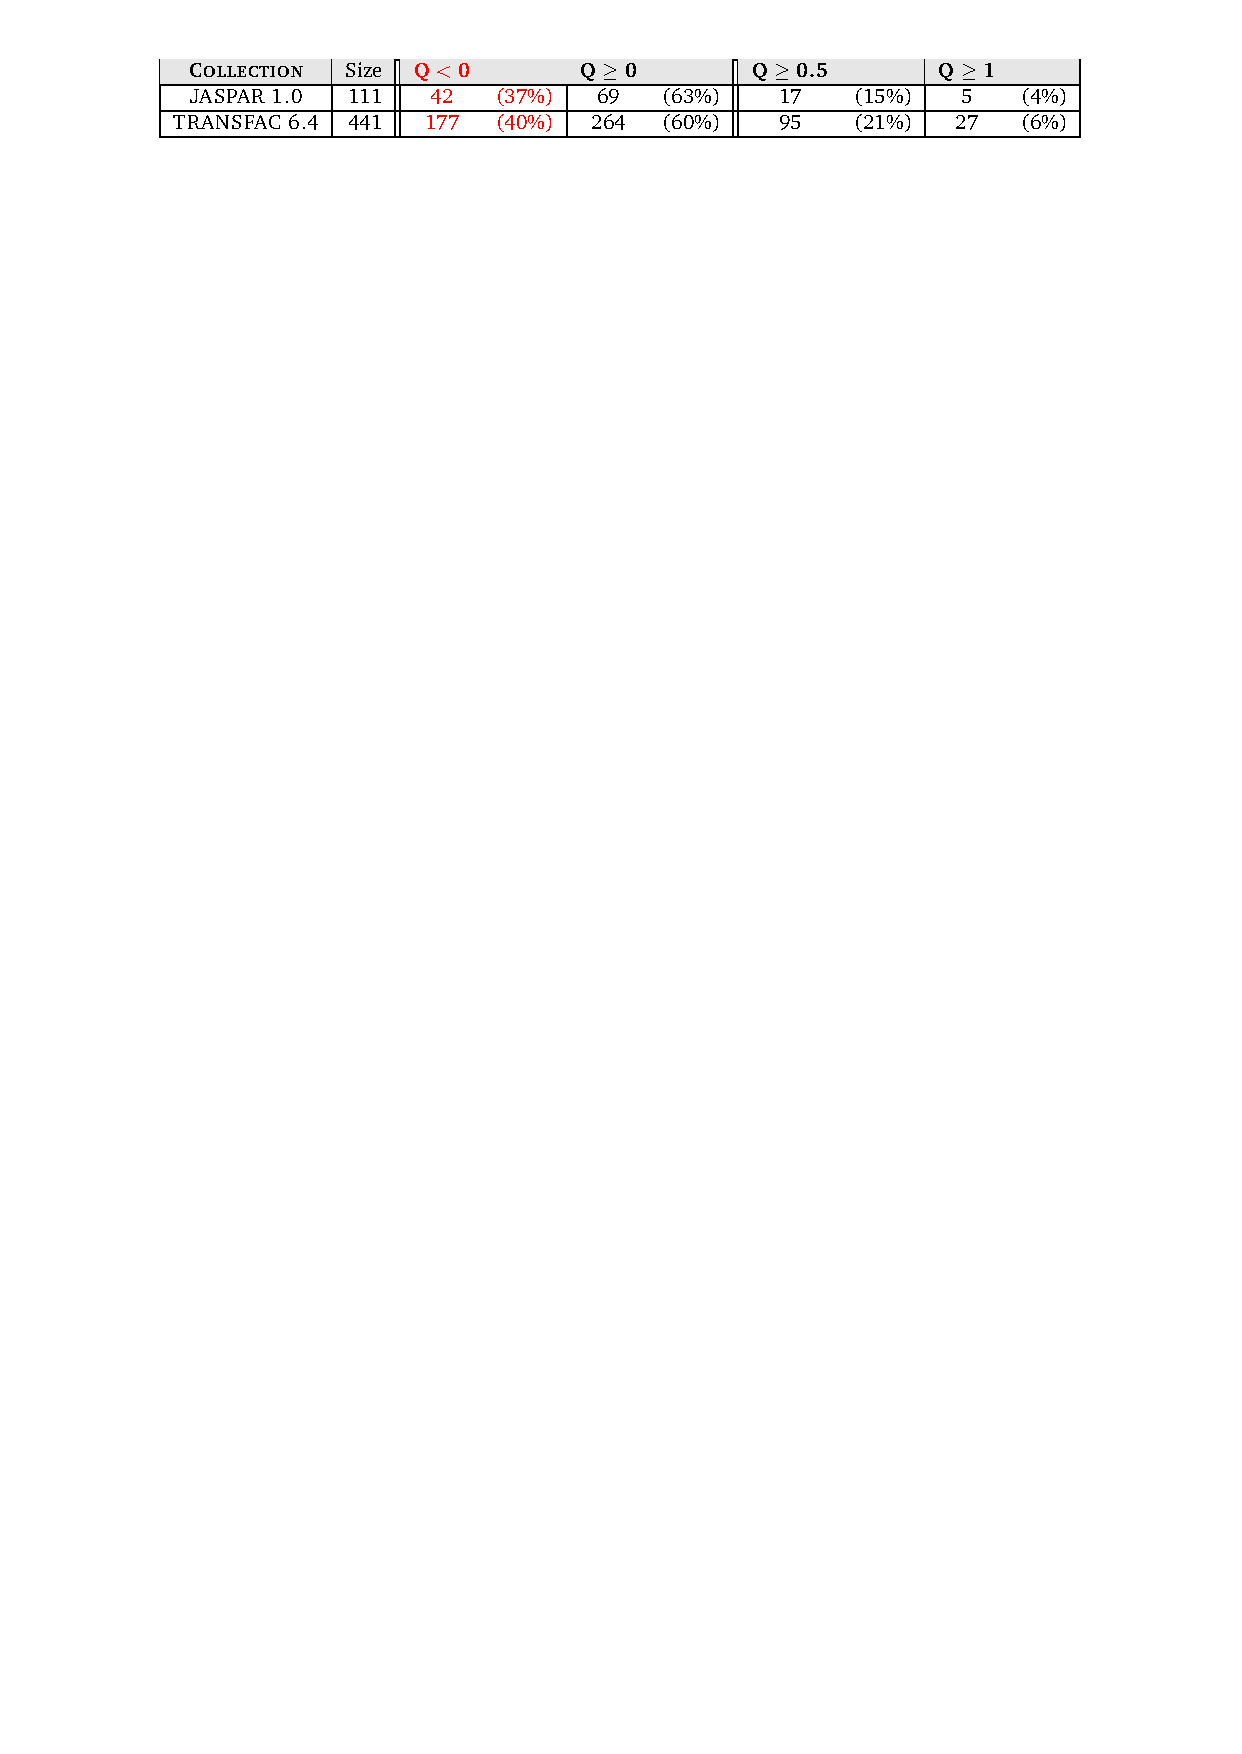
\includegraphics[bb=74 775 522 816,clip]{tables/qvalue}}
\end{center}
\end{minipage}
\mycaption{tab:qmatrices}% label
          {$Q$-value and PWM matrix specificity}% lof
          {$Q$-value and PWM matrix specificity in \db{Jaspar} and \db{Transfac}.}% caption header
          {}
\end{center}
\end{table}

Several conclusions can be extracted, therefore, from this simple test:
\begin{enumerate}
\item
Up to 40\% of the matrices from popular matrices repositories are prone to predict the same 
number of TFBSs either in human promoters or in protein coding sequences. Therefore, analysis 
with these models must be very carefully evaluated.
\item
Although a high information content normally implies better specificity of the matrices, 
there are cases in which both characteristics are not related.
\item
The use of complete collections to analyze homologous promoters usually produces the
recognition of artefactual sequence conservations as shown when the matrices are
applied on protein coding regions or intron sequences.
\item
To locate the actual common regulatory elements in a set of co-expressed sequences, it is
advisable to restrict the search using smaller collections of matrices. A simple procedure
to detect those matrices that consistently appear more frequently in a set of co-regulated
genes than in a negative control set can provide interesting results.
\item
Many of the numerous drawbacks of the weight matrices such as redundancy and low specificity
are caused by the simplicity of the model. Therefore, the use of more complex models to incorporate
additional information will obviously improve future predictions. However, we also suggest a more
rational application of the current systems to enhance the advantages and to mask the inconveniences
of these representations.
\end{enumerate}


%%%%%%%%%%%%%%%
%%% TABLE 7
%%%%%%%%%%%%%%%
\begin{table}[t!]
\begin{center}
\begin{minipage}{0.98\linewidth}\setlength{\parindent}{0pt}
\begin{center}
\scalebox{0.75}{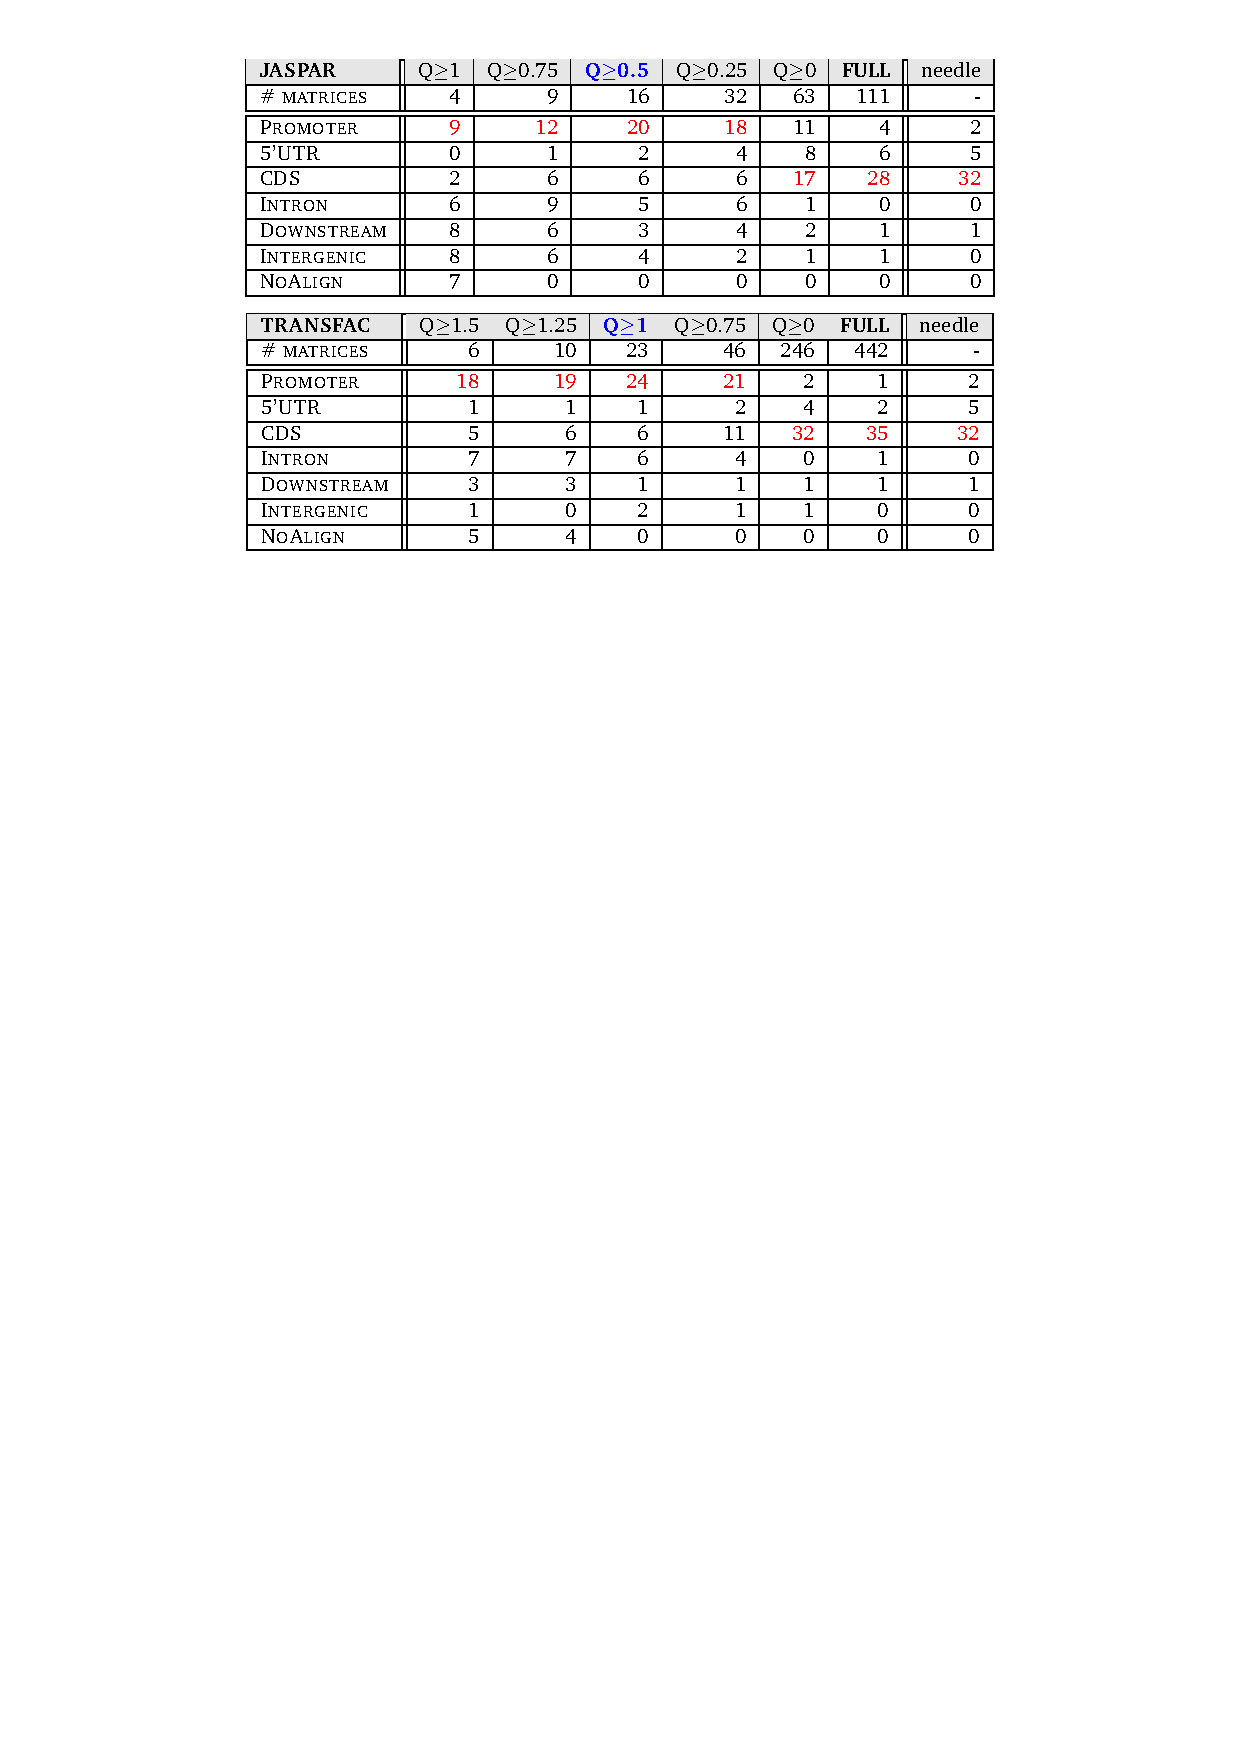
\includegraphics[bb=115 574 480 817,clip]{tables/qvalue2}}
\end{center}
\end{minipage}
\mycaption{tab:qmatrices2}% label
          {Evolution of the matrix specificity}% lof
          {Matrix specificity in several subsets of \db{Jaspar} and \db{Transfac}.}% caption header
          {}
\end{center}
\end{table}

%\sectiongreen{Meta-alignment in other scenarios}
%- IMPORTANTE: Este es un algoritmo generico que procesa cualquier tipo de informacion
%- hacer pruebas sobre ejemplos de datos en otros ambitos: AFIS, comparar otro tipo de mapas,
%comparacion de imagenes para extraer patrones????

\sectiongreen{Local TF-map alignments}

\index{TF-map alignments!loctf@local}
Local alignments are very useful to identify short stretches of a sequence that
are conserved in another one, despite the rest of both sequences is probably different. 
Local comparisons are also interesting mechanisms to locate the location (if any) of
a short composite (cluster of TFBSs, a super-pattern of TFBSs) in a long TF-map 
(see Figure \ref{fig:ttrc}). 

Two alternative designs were presented in Chapter \ref{sec:algorithms} (Section \ref{sec:local})
to implement a sequence local alignment according to the scoring function: similarity or
distance. Based on them, we present here two different implementations to identify local 
meta-alignments between two TF-maps.

\subsectionblue{Local TF-map alignments using similarity}

In a short communication, \citet{smith:1981c} published a slight modification of the 
\citeauthor{needleman:1970a} algorithm, as revisited by \citet{smith:1981b}, to deal with 
local alignments. The main objective is to find the pair of segments, one from each of two 
long sequences, such that there is no other pair of segments with greater similarity (homology).

The basic rationale of this strategy is the following: let $S(i,j)$ a position in the dynamic
programming matrix. The best local alignment ending at $S(i,j)$ is computed according to the 
three adjacent values in the matrix $S$ as long as the incorporation of one of these elements 
does not produce an alignment with negative homology. In that case, the score of the alignment 
ending at $S(i,j)$ is set to $0$. The traceback procedure then starts from the matrix cell 
having the maximum similarity, constructing the best local alignment until a cell that contains
a $0$ is reached.

%%%%%%%%%%%%%%%
%%% TABLE 8
%%%%%%%%%%%%%%%
\begin{table}[t!]
\begin{center}
\begin{minipage}{0.98\linewidth}\setlength{\parindent}{0pt}
\begin{center}
\scalebox{0.8}{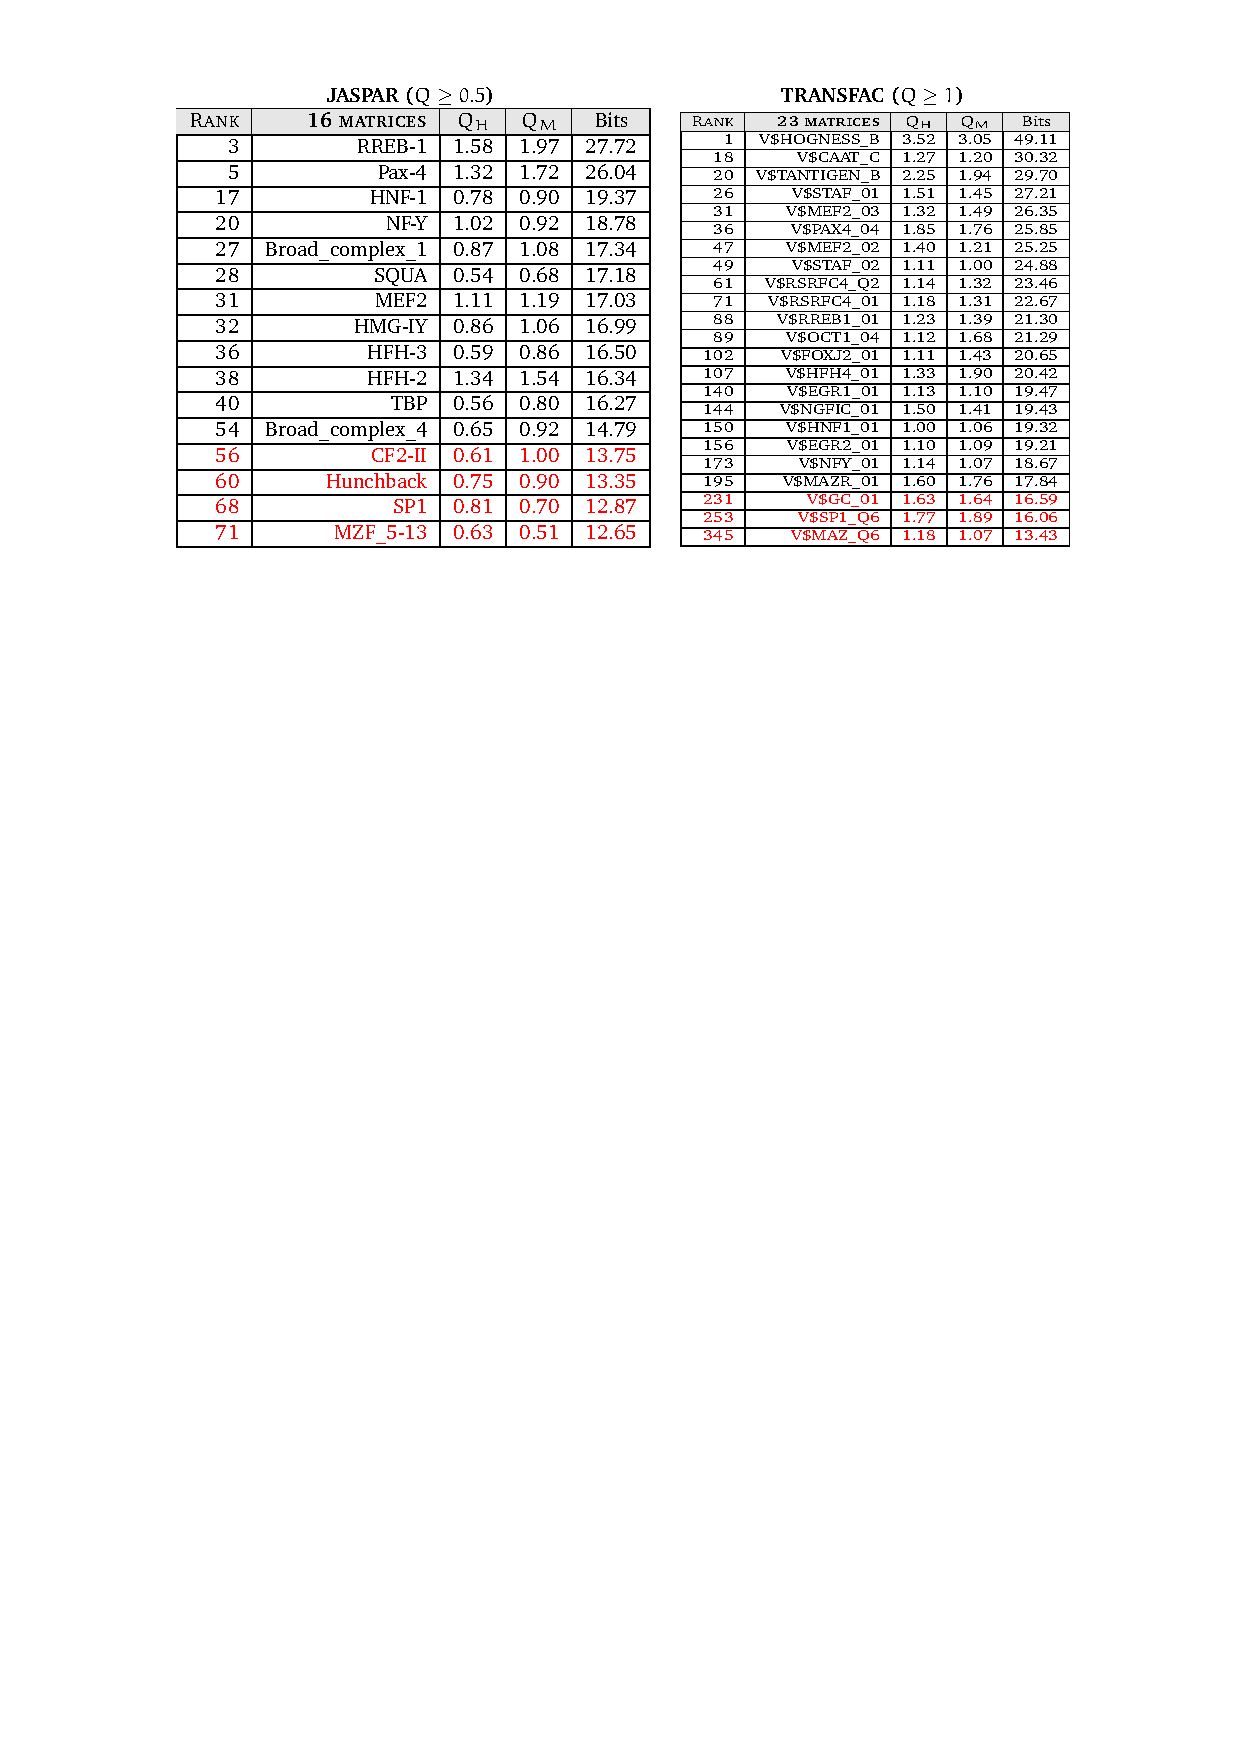
\includegraphics[bb=82 578 518 817,clip]{tables/qcolls}}
\end{center}
\end{minipage}
\mycaption{tab:qcollections}% label
          {\db{Jaspar} and \db{Transfac} specific subsets}% lof
          {\db{Jaspar} and \db{Transfac} specific subsets.}% caption header
          {In red, the matrices that are not among the most informative ones.}
\end{center}
\end{table}

The application of this approach to the meta-alignment is trivial. We can rewrite the
Equation \ref{eqnaive} introducing the $0$ in the appropriate place to produce the local alignment.
Thus, the maximum local similarity $S_{ij}$ between TF-maps  $A = a_1 \ldots a_i$ and 
$B = b_1 \ldots b_j$ where the site $a_i^f$ is equal to the site $b_j^f$, 
can be computed as: 

\begin{center}
\fcolorbox{white}{verylightgreen}{
\begin{minipage}[][][c]{0.95\linewidth}
\begin{equation}
\begin{array}{lllll}
S_{ij} \equiv & S(a_i,b_j) = & max \{0,& \alpha (a_i^s + b_j^s) +& \\
              & & &  max_{i',j'} & \{S_{i'j'}\\
              & & & \scalebox{0.7}{\mbox{$0 < i' < i$}} & - \lambda (i - i' - 1 + j - j'- 1)\\
              & & & \scalebox{0.7}{\mbox{$0 < j' < j$}} & - \mu (|(a_i^{p_1} - a_{i'}^{p_1}) - (b_j^{p_1} - b_{j'}^{p_1})|)\}\}.\\
              & & & \scalebox{0.7}{\mbox{$a_{i'}^{p_2} < a_i^{p_1}$}} & \\
              & & & \scalebox{0.7}{\mbox{$b_{j'}^{p_2} < b_j^{p_1}$}} &  
\end{array}
\end{equation}
\label{eqlocal}
\end{minipage}}
\end{center}

If we save the $N$ positions in $S$ that have the best score, we can report the best $N$ local
alignments or blocks between $A$ and $B$. The cost of the algorithm is the same as in the
global TF-map alignment algorithm, as no additional operations are necessary.

\subsectionblue{Local TF-map alignments using distance}

Despite the solution to the problem of local meta-alignment using similarity is simple
and clear, we also decided to investigate the form to produce local alignments under
the original distance scheme framework \citep{waterman:1984c}. We have taken advantage of
this research to study in depth the distribution of the scores (distance) in the meta-alignments.

As reviewed in Chapter \ref{sec:algorithms} (Section \ref{localdist}) the solution
developed by \citet{smith:1981c} to produce local alignments using a similarity
scoring function can not be directly applied in the case of the distance metric.
\citet{goad:1982a} defined the mismatch density of the alignment between two segments as 
the ratio of the minimum distance $D$ between both sequences and the length $L$ of such 
an alignment. Thus, only those alignments with a mismatch density below a certain positive 
threshold $T$ should be reported.

Formally, we are interested in those paths in the dynamic programming distance matrix
such that the mismatch density on them is minimal. The length of these alignments is a 
priori unknown and can be variable. The value of the threshold $T$ is different for each 
input, having a statistical and biological meaning at the same time.


%%%%
% Figure 17: GFF2PS: localizar un patron en una entrada
%%%%
\begin{figure}[t!]
\begin{center}
\setlength{\fboxsep}{0pt}
\fbox{\incgraph{width=0.7\linewidth}{ps/ttrc}}
\mycaption{fig:ttrc}% label
          {Using local meta-alignment in pattern identification}% lof
          {Using local meta-alignment to identify known patterns in orthologous sequences.}%header
	  {(Top) TF-map obtained with \db{Jaspar}$_{TOP50}$ on the chicken promoter of the TTR gene, 
           and a second map of three experimentally verified TFBSs in the human ortholog. 
           (Bottom) The local alignment between both maps identifies the putative 
           location of the human sites in chicken.}
\end{center}
\end{figure}

This is the procedure we follow to obtain the local meta-alignment between two maps $A$ and $B$
(see Figure \ref{fig:locprot}):

\begin{menumerate}
\item
Compute the global alignment of both maps (distance metrics), to fill the 
dynamic programming matrix $D$ in. Each position $D(i,j)$ contains the 
minimum distance in terms of a meta-alignment between the map $A = a_1 \ldots a_i$ 
and the map $B = b_1 \ldots b_j$. 
\item
Compute the matrix $\Delta D$ from $D$. For each two consecutive nodes in the
matrix $D(i,j)$ and $D(i',j')$ that are part of a path, we compute the increase 
of the distance value produced by adding the second match after the first one:

\begin{center}
\fcolorbox{white}{verylightgreen}{
\begin{minipage}[][][c]{0.95\linewidth}
\begin{equation}
\Delta D(i,j) = D(i,j) - D(i',j') ~\mbox{where}~ i' < i, j' < j.
\end{equation}
\end{minipage}}
\end{center}

\item
Define the threshold $T$ according to the $\Delta D$ values in the alignments
of length $L=2$ TFBSs. We define this threshold taking into account that
the distribution of the distance in such alignments follows the Gumbel
or extreme-value distribution (see Figure \ref{fig:glocal}). The Gumbel
function is defined as:

\begin{center}
\fcolorbox{white}{verylightgreen}{
\begin{minipage}[][][c]{0.95\linewidth}
\begin{equation}
y = e^{-x-e^{-x}} ~\mbox{where}~ P(x<0) = 0.368, P(x>0) = 0.632.
\end{equation}
\end{minipage}}
\end{center}

We are interested in defining $T$ such that a small fraction of the smallest 
values is selected. The normalization of a Gumbel function is computed as:

\begin{center}
\fcolorbox{white}{verylightgreen}{
\begin{minipage}[][][c]{0.95\linewidth}
\begin{equation}
z = \lambda (x - \mu) ~\mbox{where}~ \lambda = \frac{1.285}{\sigma}, \mu = \overline{x} - 0.45 \sigma.
\end{equation}
\end{minipage}}
\end{center}

$\overline{x}$ and $\sigma$ are the mean and the deviation of the distance values computed for 
the current set of paths, respectively. If we are considering the values $P(z \leq Z) = 0.05$,
that is under 5\% of the area covered by $z$, then:

\begin{center}
\fcolorbox{white}{verylightgreen}{
\begin{minipage}[][][c]{0.95\linewidth}
\begin{equation}
\begin{array}{c}
z = \frac{1.285 \cdot x - 1.285\cdot \overline{x} -1.285 \cdot 0.45 \sigma}{\sigma}\\
G(P) = -ln (ln (\frac{1}{p}) ~\mbox{where}~ p = 0.05, \mbox{(value of $z$)}.
\end{array}
\end{equation}
\end{minipage}}
\end{center}

For each alignment input, we will have a different $\overline{x}$ and $\sigma$ values
that, according to this equation, will provide a threshold $T$ to obtain only the
5\% of the minimal distance alignments of length $2$.

\item
Finally, trace back the paths ending at each match in the $\Delta D$ matrix. The
rule to extend a local alignment takes into account a weighted version of the
mismatch density value. A new match is added to the path if the accumulated distance
is below $T$:

\begin{center}
\fcolorbox{white}{verylightgreen}{
\begin{minipage}[][][c]{0.95\linewidth}
\begin{equation}
\frac{\Delta D(i,j)}{l} < T
\end{equation}
\end{minipage}}
\end{center}

where $l$ is the length of the current local alignment path. Visited nodes are marked up 
to be skipped in future path extensions (avoid overlapping of the solutions).
\end{menumerate}

%%%%
% Figure 18: Protocol for local alignment (D)
%%%%
\begin{figure}[t!]
\begin{center}
\setlength{\fboxsep}{0pt}
\begin{tabular}{ccc}
1 & 2 & 3\\
\fbox{\incgraph{height=4cm,width=0.3\linewidth}{ps/posterloc1}} &
\fbox{\incgraph{height=4cm,width=0.3\linewidth}{ps/posterloc2}} &
\fbox{\incgraph{height=4cm,width=0.3\linewidth}{ps/posterloc3}}\\
\end{tabular}
\mycaption{fig:locprot}% label
          {Local meta-alignment using the distance metric}% lof
          {Local meta-alignment using the distance metric}% header
          {(1) Global alignment of both maps. 
           (2) Compute the $\Delta D$ matrix for $L=2$.
           (3) Extend the best local paths with the score below $T$.}
\end{center}
\end{figure}

\sectiongreen{Discussion}

Much of the biology of the past decades has been based on the
technological advances that have accelerated our ability to sequence
DNA and proteins. It is certainly in the sequence of the genome where
the biological traits of organisms are encoded. While we have a
relatively good understanding of some of the basic mechanisms involved
in the processing of the information encoded in the DNA sequence, it
is in general very difficult to predict the biological traits --even at
the molecular level-- from the nucleotide sequence alone. Gene
promoters are a case in point: while the sequence of the promoter is
likely to contain most of the information to control the expression of
a gene, it is currently impossible to predict the expression pattern
of a gene from the analysis of its promoter sequence alone.

%%%%
% Figure 19: Gumbel distribution
%%%%
\begin{figure}[t!]
\begin{center}
\setlength{\fboxsep}{0pt}
\begin{tabular}{cc}
\incgraph{height=8cm,width=0.45\linewidth}{ps/gumbelloc1} &
\incgraph{height=8cm,width=0.45\linewidth}{ps/gumbelloc2}\\
\end{tabular}
\mycaption{fig:glocal}% label
          {Gumbel distribution of local meta-alignments}% lof
          {Gumbel distribution of local meta-alignments.}% header
          {(Left) The Gumbel generic function. (Right) TF-map alignment scores in a real pair of promoters.}
\end{center}
\end{figure}

While inferring function directly from sequence is thus far from
trivial, it is still true, that because sequence encodes function, 
similar sequences often encode similar functions. Sequence comparisons,
therefore, are an extraordinary tool to infer functional relationships: 
through sequence comparisons the function of known sequences can be 
extrapolated to newly obtained ones, and the specific sequence motifs 
can be identified responsible for the common functionality of a set of
sequences. But sequence comparisons have limitations: often
similar functions are encoded by diverse sequences. Again,
gene promoters are a case in point: many TFs bind to
sequence motifs which do not show sequence conservation. Thus, while
through phylogenetic footprinting, conserved regulatory motifs have
been in occasions uncovered in the promoters of orthologous genes
\citep{blanchette:2002a,lenhard:2003a}, searching for common patterns through the comparison of
promoter sequences in sets of co-regulated genes --as, for instance,
those resulting from microarray experiments-- is usually a frustrating
exercise. 

Here, we have attempted to address this limitation implicit in sequence
comparisons, by annotating the primary sequence with predicted
functional domains, comparing the resulting annotations instead of the
underlying primary sequence. If functional domains are encoded by
diverse sequences, the comparison and alignment of the annotation may
be more revealing of the functional relationships between sequences
and of the specific domains involved in the common functionality than
the comparison and alignment of the primary sequence. In particular,
we have attempted this strategy for the comparison and
characterization of promoter regions from genes with similar
expression patterns. We have annotated the sequence with predictions
of TFBSs --using a variety of popular tools and databases-- and identified 
the predicted sites with the labels of the corresponding TFs. We have then
compared and aligned the resulting sequence of labels. Because TFs can
bind to sites that show no sequence conservation, their labels can be
aligned which correspond to domains that, while exhibiting similar
functions, may not show sequence conservation. 

Precedents of this approach can be found in the literature.
\citep{quandt:1996a}, for instance, distinguish explicitly between
first-level analysis of promoters, in which the nucleotide sequence
is directly interrogated for the presence of regulatory motifs, and
second-level methods, in which basic higher order patterns can be
defined from a number of correlated first-level units. This
approach is further developed in \citep{frech:1997a} and
\citep{klingenhoff:1999a}, where more complex composite patterns are derived
capturing the functional organization of individual regulatory elements,
and are then used to identify and characterize related promoter
regions in absence of sequence conservation. 
Here, we go one step further, and infer automatically the composite patterns by
explicitly aligning the sequences of labels corresponding to TFs for
which binding sites have been predicted in the compared promoters (the
second-level annotation).

To align these sequences of labels--to which we refer as TF-maps--
we have stated the problem as a restriction enzyme map alignment, and
adapted a dynamic programming algorithm developed by \citet{waterman:1984c}. 
This algorithm, as well as ours, belong to a larger class of map
alignments algorithms (see also, \citep{miller:1990a,miller:1991a,myers:1992a,huang:1992a}). 
In typical alignments, the sequences are of labels
denoting either nucleotides or amino acids. In map alignments, the
sequences are of pairs (label,integer), where the label denotes a
predicted domain or site (possibly exhibiting some behavior or functionality), 
and the integer the position on the primary sequence where the domain or the 
site has been predicted. In global pairwise sequence alignments, the goal is to
obtain the alignment that maximizes the sum of the scores of the
aligned positions --given the score of the individual alignments of
all possible pairs of labels. In contrast, in map alignments, only
positions with identical labels can be aligned and the goal is to
obtain the largest common subsequence constrained to minimize the
differences in distances on the primary sequence between consecutive
aligned positions. Sequence and map alignments can be generalized to a
broader class of alignments that includes both. 

Map alignments have been mostly used to align restriction enzyme
maps. In this case, the label denotes a restriction enzyme, and the
integer the position on the primary sequence of the site recognized by
the enzyme. \citet{waterman:1984c} first established the concept of
map alignment and provided an algorithm for computing the optimal
alignment of two maps. Later \citet{myers:1992a} described an improved
algorithm to efficiently find map alignments which relies on the
extreme sparsity of the dynamic programming matrix in \citep{waterman:1984c}
--the result of the match state being defined only between identical labels. 
\citet{miller:1990a,miller:1991a} introduced new algorithms that permitted
the efficient search of a long map for the best matches to a shorter probe map.
\citet{huang:1992a} generalized these algorithms to deal with different map errors. 

In our case, the label denotes a TF, and the integer the initial
position on the primary sequence where a binding motif for the TF has
been predicted. There are, however, two important differences between
restriction enzyme maps and TF-maps. First, while prediction of
restriction sites is deterministic, producing a binary output
(``site'', ``no site''), prediction of TFBSs is often probabilistic
and predicted sites may have an associated score. The score can
usually be related to the strength of the binding of the TF to the
site \citep{stormo:2000a}. Since, it makes sense, therefore, to prefer
in TF-map alignments higher scoring sites, the score of the TFBSs needs
to be taking into account when building optimal TF-map alignments.
Second, enzyme restriction sites are single-nucleotide positions on
the primary sequence. TFBSs, in contrast, are sequence intervals, and
have thus, in addition to position, an associated length. Because we
explicitly prohibit overlap between aligned elements, we can not
directly extrapolate the algorithm of \citet{myers:1992a}. However, as
in their approach, we have also taken advantage of the extreme
sparsity of the dynamic programming matrix to implement an efficient
algorithm that, in our experience, is comparable in efficiency. There
is another important feature characteristic of our approach that,
while it does not influence the algorithmic strategy, it is essential
to its success. As we have already stressed, we do not label the site,
but the function of the site. That is, we do not label the TFBSs, but
the TFs that bind to the sites. This allows for significant functional
alignments even in the absence of sequence conservation.

We have estimated the optimal parameters of the algorithm in a small,
but well annotated, set of orthologous human-mouse genes. We used three
popular collections of PWMs for TFBSs (\db{Jaspar} 1.0 \citep{sandelin:2004a}, 
\db{Promo} 2.0 \citep{farre:2003a} and \db{Transfac} 6.3 \citep{matys:2003a}) to 
obtain the TF-maps of the promoter sequences. Results on this data set 
indicate that, by dramatically reducing the overwhelming number of 
spurious predictions of TFBSs produced using these collections, 
TF-map alignments are able to successfully uncover the few conserved 
functionally active regulatory domains. 
Differences can be observed between the performance of the
different collections of TFBSs; alignments obtained using \db{Jaspar}  
--and, in particular, using a subset consisting of the 50 top most informative
matrices-- appear to show the optimal balance between sensitivity and
specificity. The data set that we have used, however, is too small to
infer general trends on the comparative behavior of these collections.

Interestingly, despite the stronger sequence conservation between
protein-coding regions, TF-map alignments score the highest between promoter
regions in the training set of orthologous human-mouse genes. 
This indicates that TF-map alignments are able to pick up regulatory
signals that sequence alignments can not. Results in an independent
larger data set of co-regulated genes from the CISRED database are
also in support of this conclusion: we have been able to obtain more
significant alignments between the TF-maps than between the nucleotide
sequences of the promoters of co-regulated genes. Results in CISRED are
certainly not extraordinary. Both sequence and TF-map alignments
perform very poorly when detecting relationships between co-regulated
gens in CISRED. Only in 97 out of 5333 gene representatives in CISRED
(1.8\%), TF-map alignments scored significantly higher for co-regulated 
than for non co-regulated genes. Using BLASTN, this number was only 11
(0.2\%). Finding relationships between the promoters of the genes
co-regulated in CISRED is a task as challenging as one can
imagine. The CISRED collection of high-confidence co-expressed genes
is not derived from overall conservation, or from co-occurrence of motifs, 
in the sequence of the gene promoters. CISRED co-expression is derived 
instead from cDNA microarray, SAGE and other high-throughput gene expression 
monitoring techniques. CISRED co-expression clusters are thus a mixture of directly
and indirectly co-regulated genes and one would then expect only a few
genes within each cluster --maybe in a few subsets-- to share
functionally equivalent motifs in their promoter sequences. The poor
performance of TF-map alignments, however, could also be reflecting the
incompleteness of the current collections of TFBSs, and how little we
know of the molecular rules governing the expression of human genes. 

On the other hand, while building global pairwise alignments maybe
appropriate to compare promoter sequences of orthologous human-mouse
genes, to compare sequences from multiple genes weakly
co-regulated --such as those in CISRED-- multiple and/or local alignments
may be more effective in capturing the functional motifs underlying
co-expression. Indeed, from a multiple TF-map alignment of promoters
of a set of co-regulated genes, a ``transcriptional regulatory
super-pattern'' \index{super-pattern}
can be derived capturing those elements conferring
expression specificity. Using a local alignment search algorithm, the
super-pattern can then be used to identify additional genes or
transcripts belonging to the same expression class (see other approaches
in \citep{knight:1995a}). 

Even more appropriate to the analysis of sets of weakly co-expressed genes (that
is, including genes both directly and indirectly co-regulated), such
as those in the CISRED clusters, would be the extension of the
unsupervised pattern recognition techniques usually applied to motif
discovery in DNA sequences (in programs such as MEME
\citep{bailey:1994a}, AlignAce \citep{roth:1998a} and others (see
\citep{tompa:2005a}, for a recent comparative evaluation) to motif
discovery in TF-maps. This would allow for the identification within a
co-expression cluster of different ``transcriptional regulatory
super-patterns''.  These super-patterns, in turn, and the subclusters
they induce, could contribute to sort out direct vs. indirect
co-regulation effects within the cluster. These and other extensions
to the TF-map alignments (for instance, those allowing to deal with
non-colinear arrangements of TFBSs that have been indeed observed in
orthologous genes, see next chapter) are all feasible, and will
certainly contribute to the discriminatory power of TF-map comparisons
and alignments.

In summary, our results suggest that comparisons of annotations of
higher order domains can, in occasions, be more meaningful to
characterize the underlying functionality of sequences, than direct
comparisons at the very primary sequence level. Here we have explored
these strategies for the characterization of the promoter regions of
co-regulated genes, and we have annotated the primary sequence of them
with predictions of TFs. Moreover, we have also used the discriminative 
power of TF-maps for a better identification of orthologous promoter 
regions along large genomic sequences (e.g. chromosomes). In addition,
we measured the specificity of PWMs in protein coding sequences and 
promoters.

However, we can imagine similar strategies to
address many other problems in sequence analysis. One can imagine, for
instance, annotating protein sequences with PFAM domains
\citep{bateman:2004a}, and compare the resulting annotations to detect
distant functional relationships between proteins and protein
families. Or annotating genome sequences with the Gene Ontology (GO,
\citep{tgoc:2000a}) labels of the genes encoded in these sequences,
and aligning the GO labels to detect clusters of conserved functions
across genomes. In fact, the annotation of the primary sequence with
higher order domains to improve alignments has been often explored.  
For instance, to compare protein secondary structures, or to
anchor whole genome alignments \citep{batzoglou:2000a}, or
even alignments of promoter regions \citep{berezikov:2004a}. In all
these cases, however, the ultimate goal is to obtain an optimal
sequence alignment either between the original primary sequences, or
between the 1-1 mappings of the primary sequence into a reduced
alphabet (for instance, denoting secondary structure elements). We
believe that, as the molecular functionality of the primary sequence
becomes better understood, comparisons between higher order
annotations, such as those performed here, in which the primary
sequence is completely abstracted, may become increasingly relevant.

%%%%%%%%%%%%%%%%%%
%%% References for this chapter
%%% ENCERRAR ENTRE LLAVES PARA EVITAR PROBLEMAS
\bibliographystyle{plainnat}
{\bibliography{sections/bibliography}}
  % TF-map alignment 
    \clearemptydoublepage

    %%%%%%%%%%%%%%%%%%%%%%%%%%%%%%%%

% Multiple Non-Collinear TF-map
% Alignment of Promoter Regions

%%%%%%%%%%%%%%%%%%%%%%%%%%%%%%%%

\chapter[Multiple Non-Collinear TF-map Alignment]
{\textbf{M}ultiple Non-Collinear\\ TF-map Alignment}\label{sec:mma}
\sectiongreen*{Summary}
\begin{center}
\begin{tabular}{c}
\fcolorbox{blue}{verylightgrey}{
\begin{minipage}[][4cm][c]{0.8\linewidth}
\sffamily
The generalization of the pairwise TF-map alignment is presented here. First, the 
formal definition of a multiple map alignment and how to compute the optimal score
is provided. Next, we use a progressive approach to build up a multiple alignment in
a stepwise manner. Then, we have studied how to break the non-collinearity property 
inherent to the alignments produced by dynamic programming techniques. Results
on biological data indicate that multiple TF-map alignments are able to locate regulatory
elements in several promoters that are not conserved at sequence level.
\end{minipage}}\\
\\[2ex]
\begin{minipage}[][4cm][c]{0.9\linewidth}
\minitoc
\end{minipage}
\end{tabular}
\end{center}
\newpage


\sectiongreen{The need for multiple TF-map alignment}\label{sec:motiv}

% A. (MULTIPLE) SEQUENCE ALIGNMENT IS IMPORTANT
\lettrine[lines=4,loversize=-0.1,lraise=0.1,lhang=.2]{S}{equence comparisons are 
one of the most important computational tools} in molecular biology. Sequences are 
good symbolic representations of biological molecules that encode relevant information 
about their structure, function and history. From the analysis of several related sequences, 
biologically significant facts can be inferred. For instance, genomic sequence comparisons
are performed in order to identificate genes or regulatory sites across
different genomes, as these functional elements tend to exhibit 
conservational patterns different from those observed in regions that are not 
functional.

%B. MULTIPLE SEQUENCE ALIGNMENT: PROGRESSIVE
In attempt to allow for multiple sequence comparisons, the basic dynamic
programming recurrences introduced in the 1970s to align efficiently two
sequences of $n$ symbols in $O(n^2)$ \citep{needleman:1970a,sellers:1974a},
can be naturally extended for $k$ sequences, with an exponential cost
$O(n^k)$ \citep{waterman:1976a}. As this cost is unaffordable in practice,
many heuristics have appeared to provide acceptable solutions with a minor cost.
The most popular of them is the hierarchical or clustering method
\citep{feng:1987a,thompson:1994a}. 

This procedure, also called progressive alignment, is a greedy algorithm
that runs in $O(k^2 n^2)$ time. In a first step, this method performs all
of the pairwise alignments to build an evolutionary tree. In a second step,
an initial alignment is constructed from the two closest sequences,
incorporating then the rest to the profile following the guide tree. Such a
procedure does not guarantee to find the optimal solution in mathematical
terms. However, the results are generally in good agreement with the
biological problem of aligning correctly bases of homologous functional
elements. See Chapter \ref{sec:algorithms} Section \ref{sec:msa} for a 
comprehensive review of this topic.

Progressive alignment has also commonly used in the genome-wide
alignment methods that perform rapid multiple genomic alignments to identify
conserved biological features between distant species. Basically, these
algorithms identify local similarities between two genomes that are then
used as anchors to align the interleaving regions \citep{delcher:1999a}.
The progressive technique is then combined with these genome pairwise
aligners to build up the multiple genome alignment \citep{brudno:2003a,bray:2004a}.

% C. THINGS ARE NOT ALWAYS CONSERVED AT THE SEQ LEVEL
These comparisons at the sequence level have limitations however. Although
similar sequences do tend to play similar biological functions, the opposite
is not necessarily true. Often similar functions are encoded in higher order
sequence elements that are not necessarily conserved at the sequence level.
As a result, similar functions are frequently encoded by diverse sequences
which are undetectable by conventional sequence alignment methods.

% D. PROMOTERS
Gene promoter regions are a good example. The information that governs the
RNA synthesis is mostly encoded in the gene promoter, a region normally $200$
to $2,000$ nucleotides long upstream of the transcription start site of the gene (TSS).
Transcription factors (TFs) bind to sequence specific motifs (the TF binding
sites, TFBSs) within the promoters. TFBSs are $5-8$ nucleotides long and one
promoter region contains on the order of $10$ to $50$ of them \citep{wray:2003a}.
Such motifs appear to be arranged in specific configurations that define the
temporal and spatial transcriptional pattern program of each gene. Genes
presenting similar expression patterns are assumed to share similar
configurations of TFBSs in their promoters. However, TFBSs associated to
the same TF are known to contain sequence substitutions, being in many
cases completely different. Promoter regions of genes with similar
expression pattern may not be similar at the sequence level, even though
they may be co-regulated.

% E. PREVIOUS WORK
In the previous chapter \citep{blanco:2006b}, we suggested the existence of 
regulatory information conserved between related promoters that could not be 
detected at the sequence level. Let $\Sigma_{TF}$ be the alphabet of TFs denoting
symbols. We initially defined the process of mapping a nucleotide sequence into a 
sequence in $\Sigma_{TF}$ (the TF-maps). Then, we developed an efficient algorithm 
to obtain the global pairwise alignment between two TF-maps \citep{blanco:2006b}. 
Finally, we showed the TF-map alignments were more accurate than conventional sequence 
alignment to distinguish pairwise gene co-expression in a collection of microarray 
results \citep{blanco:2006b}.

%%%%
% Figure 1: dummy mapping
%%%%
\begin{figure}[t!]
\begin{center}
\setlength{\fboxsep}{0pt}
\fbox{\incgraph{width=0.65\linewidth}{ps/dmapping}}
\mycaption{fig:dmapping}% label
          {TF-mapping in a simple example}% lof
          {TF-mapping in a simple example.}% caption header
          {}
\end{center}
\end{figure}

% F. PRESENT THIS PAPER 
In this chapter, we present an efficient implementation of
the multiple TF-map alignment based in the progressive alignment paradigm.
We have introduced some modifications in the pairwise global TF-map alignment
algorithm to align two clusters of TF-maps, eventually allowing non-collinear
arrangements of TFBSs in the results without additional cost. Most dynamic
programming global alignments rarely cope with the presence of rearrangements
observed in the DNA, being only partially identified by combining global and
local alignment strategies \citep{brudno:2004a,darling:2004a}. This problem is
particularly relevant in the case of the regulatory regions, where
non-collinear configurations of TFBSs are prone to be conserved
\citep{nix:2005a}. 

% G. STRUCTURE OF THE PAPER
The structure of the chapter is the following: first, we briefly reviewed the
concept of mapping functions and provide the formal definition of a multiple
TF-map alignment. Then, we introduce the main algorithm that performs the
progressive alignment of multiple TF-maps. Next, we detail the algorithm
to compute the optimal pairwise alignment of two clusters of maps. Later,
we define formally a non-collinear alignment, introducing some
modifications in the pairwise algorithm to allow the detection of these
cases. Finally, we systematically estimate the optimal parameters of the
alignment to distinguish promoters from other gene regions in a set of well
characterized human-rodent gene pairs and their corresponding orthologs in
chicken and zebrafish. These results are compared to those obtained by
conventional sequence alignment methods, showing the validness of our approach. 
Several particular examples are presented in which multiple TF-map alignments 
characterize conserved regulatory elements that are otherwise imperceptible 
in sequence-level comparisons.

%%%%
% Figure 2: dummy real
%%%%
\begin{figure}[t!]
\begin{center}
\setlength{\fboxsep}{0pt}
\begin{tabular}{|cc|}
\hline
A & \incgraph{width=0.65\linewidth,height=3cm}{ps/oneline}\\
B & \incgraph{width=0.65\linewidth}{ps/extended}\\
\hline
\end{tabular}
\mycaption{fig:rmapping}% label
          {TF-mapping of the human promoter NM\_015900}% lof
          {TF-mapping of the human promoter NM\_015900 ($500$ nucleotides).}% caption header
          {(A) Condensed representation of the TRANSFAC predictions.
           (B) The same set of predictions displayed in a non-overlapping format.}
\end{center}
\end{figure}

%%%%%%%%%%%%%%%%%%%%%%%%%%%%
%% Definitions            %%
%%
\sectiongreen{Basic definitions}

\subsectionblue{Mapping a promoter sequence into a TF-map}

Let $\Sigma_{DNA}$ be the alphabet of four nucleotides. Let $\Sigma_{TF}$ be 
the alphabet of TFs denoting symbols. In a previous work \citep{blanco:2006b}, 
we defined a mapping function as a procedure to translate a promoter region 
$S = s_1 s_2 \ldots s_k$ where each nucleotide $s_i \in \Sigma_{DNA}$, into a
sequence of TF-tuples $M = m_1 m_2 \ldots m_n$ where each TF-tuple 
$m_i=<m_i^f,m_i^{p1},m_i^{p2},m_i^s>$ denotes the match 
of a binding site for the TF $m_i^f \in \Sigma_{TF}$ occurring between the
position $m_i^{p1}$ and the position $m_i^{p2}$ over the sequence $S$
with score $m_i^s$. Different mapping functions can be used to obtain the 
translation from $S$ to $M$ such as a collection of weight matrices representing TFBSs
(JASPAR \citep{vlieghe:2006a}, PROMO \citep{farre:2003a} or TRANSFAC \citep{matys:2006a}). 
For each match over a given threshold, we register a new TF-tuple in $M$ defined 
by the label $(m_i^f)$ of the TF associated to the PWM, the positions 
$(m_i^{p1},m_i^{p2})$ and the score $(m_i^s)$ of the match (see Figure 
\ref{fig:dmapping}, for an example). Other mapping functions can used instead, such 
as pattern discovery programs that identify a set of unknown motifs conserved 
in several promoters (e.g. MEME \citep{bailey:1994a}).

Matches are annotated at a given location irrespective of their orientation 
in which they occur. This translation preserves the order of $S$ in $M$, that 
is if $i<j$ in $M$ then $(m_i^{p1} < m_j^{p1})$. Matches to different TFs may 
possibly occur at the same position, being false positives in most cases (see 
a real example in Figure \ref{fig:rmapping}). We refer to the resulting sequence 
of TF-tuples $M$ as a Transcription Factor Map, or simply a TF-map.

\subsectionblue{Multiple alignment of TF-maps} 
\index{alignment!mtfma@multiple TF-map alignments} \index{alignment!mmeta@multiple meta-alignments}
\index{TF-map alignments!mmetatf@multiple TF-map alignments}
\index{multiple TF-map alignments}
Let $M_1,M_2,\ldots,M_k$ be a set of TF-maps where each map is denoted
as $M_i = m_{i,1} m_{i,2} \ldots m_{i,|M_i|}$ and each TFBS is
denoted as $m_{i,j}^f \in \Sigma_{TF}$. Let $M_1^*,M_2^*,\ldots,M_k^*$
be the extended set of TF-maps where each map is denoted as $M_i^* =
m_{i,1}^* m_{i,2}^* \ldots m_{i,|M_i^*|}^*$, and each TFBS is denoted
as $m_{i,j}^{*f} \in \Sigma_{TF} \cup \{-\}$. The symbol $'-'$ indicates a
gap, which can be considered as a particular TF-tuple 
$<'-',\cdot,\cdot,\gamma>$ where the value $\cdot$ is a null value 
and $\gamma$ is the penalty for introducing a gap in a column of the alignment.

The alignment of $k$ maps $M_1,M_2,\ldots,M_k$ is then a correspondence $T$, maybe empty,
among the extended maps $M_1^*,M_2^*,\ldots,M_k^*$ such that:

\begin{enumerate}
\item
The extended maps have the same length.
\item 
If the gaps are removed from each $M_i^*$, we recover $M_i$.
\item
At least one element in a column is different from a gap.
\item
The elements that are aligned in a column correspond to the same TF.
\item
No overlap in the primary sequence is permitted between adjacent sites 
in the alignment.
\end{enumerate}

Note that the first three conditions define the classical multiple alignment 
of sequences. Last two conditions, however, introduce two new constrains that 
are related to the match state and the non-overlapping property, according to the 
notion of pairwise TF-map alignment provided in \citep{blanco:2006b}.


\subsectionblue{The score of a multiple alignment of TF-maps}

A multiple TF-map alignment --or simply, a multiple map alignment (MMA),
in contrast to a multiple sequence alignment (MSA)--
can be also represented as a rectangular array:

\begin{center}
\fcolorbox{white}{verylightgreen}{ 
\begin{minipage}[][][c]{0.95\linewidth}
\begin{equation}
T = \left(
\begin{array}{llll}
m_{1,1}^* & m_{1,2}^* & \ldots & m_{1,t}^*\\
m_{2,1}^* & m_{2,2}^* & \ldots & m_{2,t}^*\\
\ldots & & & \ldots\\
m_{k,1}^* & m_{k,2}^* & \ldots & m_{k,t}^*\\
\end{array}\right),
\end{equation}
\end{minipage}}
\end{center}

\noindent where each column $T(i)= (m_{1,i}^*,m_{2,i}^*,\ldots,m_{k,i}^*)$
is the multiple match among the TF-tuples in position $i$ from 
$M_1^*, M_2^* \ldots M_k^*$. Given the multiple alignment $T$, we compute the 
score $s(T)$ of the MMA as:

\begin{center}
\fcolorbox{white}{verylightgreen}{ 
\begin{minipage}[][][c]{0.95\linewidth}
\begin{equation}
s(T) = 
\begin{array}{ll}
  & \alpha \sum_{i=1}^t{\sum_{j=1}^k{m_{j,i}^{*s}}}\\
- & \lambda (g)\\
- & \mu \sum_{\forall i,i'}{f(m_{1,i}^{*p1}-m_{1,i'}^{*p1},m_{2,i}^{*p1} - m_{2,i'}^{*p1},\ldots,m_{k,i}^{*p1}-m_{k,i'}^{*p1})}
\end{array}
\label{eq:scorem}
\end{equation}
\end{minipage}}
\end{center}

\noindent where $\alpha,\lambda,\mu>0$, $g$ is the number of columns with only one
element different from a gap in the MMA (unaligned elements), and
$f$ is a function that measures the conservation of distance between the
sites of every map in two consecutive columns ($i,i'$) with more than one aligned element in the 
MMA. That is, the score of the alignment increases with the score of the aligned elements 
and the penalty of the gaps ($\alpha$), and decreases with the number of unaligned
elements ($\lambda$), and with the difference in the distance between adjacent aligned 
elements ($\mu$). See the previous chapter and \citet{blanco:2006b} for further details 
about the TF-map alignment parameters.

%%%%%%%%%%%%%%%%%%%%%%%%%%%%
%% The Algorithms         %%
%%
\sectiongreen{The algorithms}

There are many possible alignments between a group of TF-maps. The optimal
alignment is the one scoring the maximum among all possible alignments. In
a previous work \citep{blanco:2006b}, we implemented a dynamic programming
algorithm to obtain such an alignment efficiently for the case of two
TF-maps. The optimal multiple sequence alignment problem (and therefore
also the multiple alignment of maps) is, however, much more difficult, being 
formally a NP-complete problem \citep{wang:1994a}.

Here, we propose to adapt the popular progressive alignment strategy to
the TF-map alignment. The solutions obtained by this method are
not guaranteed to be optimal. However, multiple progressive alignments 
usually have an underlying biological explanation \citep{thompson:1994a}. 
We have also introduced some changes in the basic pairwise TF-map alignment 
algorithm developed in \citep{blanco:2006b}, in order to deal now with two 
clusters of MMAs instead of two single TF-maps. 

\subsectionblue{Progressive MMA algorithm}
\index{multiple TF-map alignments!progmmeta@progressive alignment}

Let $(G_1 \ldots G_k)$ be the initial list of $k$ TF-map groups,
where each group contains a single TF-map. Let $S$ be the similarity 
matrix where $S(G_i,G_j)$ denotes the similarity between the TF-map 
groups $G_i$ and $G_j$.

The progressive MMA algorithm shown in Figure \ref{fig:mmaalg} builds up a multiple TF-map
alignment in a stepwise manner. In a first step, all pairwise TF-map
alignments are performed. The initial multiple alignment is created 
with the two most similar ones. Both maps are substituted for a
new group that contains their alignment. The similarity between this
new cluster and the rest of the TF-maps is then estimated, updating
tha $S$ matrix (see Implementation).

In a second step, an iterative procedure selects at each round the pair
of clusters that are more similar from the pool of available groups.
These two groups are aligned and merged again into a new TF-map cluster,
estimating the similarity to the remaining ones. At the end of the
process, there is only one group that contains the progressive alignment
of the input TF-maps.

The cost of the progressive MMA can be expressed in terms of the number
of pairwise TF-map alignments that must be computed. Let $k$ be the number
of maps to be aligned and $n$ be the length of each map. The initial round
performs $O(k^2)$ pairwise alignments. Next, the progressive round performs
$O(k)$ alignments involving two groups. Let $P(n)$ be the cost of each
pairwise operation, then the cost of the progressive alignment algorithm
is $O(k^2 \cdot P(n))$. The expected value of $P(n)$ is calculated in the
next section.


%%%%
% Figure 4: Progressive Multiple Map Alignment
%%%%
\begin{figure}[t!]
\begin{center}
\scalebox{1}{
\fcolorbox{white}{verylightgreen}{
\begin{minipage}[][][c]{\linewidth}
\begin{algorithmic}[5]
\REQUIRE $G$: list of TF-map groups $(G_1 \ldots G_k)$
\STATE
\STATE \COMMENT{ Initial Step: pairwise alignment all Vs all }
\STATE maxSim $\leftarrow -\infty $
\FOR{$i=1$ to $k$}
\FOR{$j=i+1$ to $k$}
\STATE $S(G_i,G_j) \leftarrow$ ComputePairwiseSimilarity$(G_i,G_j)$;
\STATE \COMMENT{Select the pair with maximum similarity}
\STATE maxSim $\leftarrow$ max(maxSim,$S(G_i,G_j)$);
\ENDFOR
\ENDFOR
\STATE \COMMENT{Create a new group: estimate the similarity to others}
\STATE $G_{iSim-jSim} \leftarrow$ MergeGroups$(G_{iSim},G_{jSim})$;
\STATE
\STATE \COMMENT{ Progressive Step: cluster the two most similar groups }
\WHILE{$|G| > 1$}
\STATE maxSim $\leftarrow -\infty $
\FOR{$i=1$ to $|G|$}
\FOR{$j=i+1$ to $|G|$}
\STATE \COMMENT{Select the pair with maximum similarity}
\STATE maxSim $\leftarrow$ max(maxSim,$S(G_i,G_j)$);
\ENDFOR
\ENDFOR
\STATE \COMMENT{Create a new group: estimate the similarity to others}
\STATE $G_{iSim-jSim} \leftarrow$ MergeGroups$(G_{iSim},G_{jSim})$;
\ENDWHILE
\end{algorithmic}
\end{minipage}}}
\mycaption{fig:mmaalg}% label
          {Progressive multiple map alignment algorithm}% lof
          {Progressive multiple map alignment algorithm.}% caption header
          {}
\end{center}
\end{figure}


\subsubsectionblue{Implementation}

In the progressive MMA algorithm shown in Figure \ref{fig:mmaalg}, the variable \emph{maxSim}
saves the maximum score so far computed at each round. The group
identifiers of such a score can easily be retrieved using a supplementary
pair of variables \emph{iSim, jSim}.

The pairwise TF-map alignment algorithm called
\emph{ComputePairwiseSimilarity} \citep{blanco:2006b} has been slightly
modified to accomodate the alignment of two TF-maps groups, as explained in
the next section. The optimal pairwise alignments between the input TF-maps
in the initial round are saved, as they could be required during the
iterative procedure.

Once a new TF-map group is created from the two most similar ones, their
binding sites must be merged (function \emph{MergeGroups}). The order of
the TFBSs in the new group must take into account the position of the
binding sites in their primary promoter sequences. In the approach here, we
do not create a profile of each MMA. Instead, all of the TFBSs of each group
are always available for subsequent TF-map alignments.

The alignments between this new TF-map group and each one of the
rest of the groups are not explicitly computed. The similarity among
them is instead estimated with the WPGMA method (Weighted Pair Group Method 
with Arithmetic Mean) according to the previous similarity between the 
groups $G_{iSim}$ and $G_{jSim}$ to the others. If an alignment between 
two groups whose similarity was estimated before is identified as the most similar 
during the progressive step, the MMA must be explicitly computed before merging 
both TF-map groups.

%%%%
% Figure 5: DP matrix
%%%%
\begin{figure}[t!]
\begin{center}
\setlength{\fboxsep}{0pt}
\fbox{\incgraph{width=0.75\linewidth}{ps/mmads}}
\mycaption{fig:mmads}% label
          {MMA algorithm: data structures and matrix}% lof
          {MMA algorithm: data structures and similarity matrix.}% caption header
          {}
\end{center}
\end{figure}


\subsectionblue{The alignment of two clusters of MMAs}
\index{multiple TF-map alignments!clusmmeta@alignment of two clusters}

Let $G_x = m_{x,1} m_{x,2} \ldots m_{x,|G_x|}$ and 
$G_y = m_{y,1} m_{y,2} \ldots m_{y,|G_y|}$ be the two most similar groups of 
TF-maps in the current round of the progressive alignment. Let $S$ be the scoring 
dynamic programming matrix where $S(i,j) = S(m_{x,i},m_{y,j})$ denotes the similarity 
of the best TF-map alignment of the groups $G_x=m_{x,1} \ldots m_{x,i}$ and 
$G_y=m_{y,1} \ldots m_{y,j}$, according to the scoring function in Equation \ref{eq:scorem}.
The \emph{ComputePairwiseSimilarity} algorithm explained here is a generalization of 
that developed in \citep{blanco:2006b} to align two TF-maps that computes the optimal 
pairwise TF-map alignment between $G_x$ and $G_y$.

This algorithm basically searches the the maps of 
both groups to find matches between one site in one group and one site in the other. 
Once a new match is identified, the previous matches must be evaluated
in order to construct the optimal alignment ending at this one (see Figure \ref{fig:mmads}).
Because this class of scoring matrices are highly sparse, 
we register the coordinates in $S$ of the matches computed previously. 
Thus, to compute the optimal score at the cell $S(i,j)$, only the 
non-empty cells in $S$ that are visible for the current match need to be accessed. 
In addition, we maintain the list sorted by optimal score, so that the cell scoring the 
maximum value is at the beginning of the list and, in most cases, only a few nodes will
need to be accessed before a critical node is reached beyond which the
optimal score can not be improved \citep{blanco:2006b}.

The number of computations $P(n)$ in this algorithm is very similar
to that obtained in the conventional pairwise TF-map alignment algorithm
\citep{blanco:2006b}. The exact complexity of this algorithm is
difficult to be studied --depending mostly on the size of the input maps
and the sparsity of the resulting marix $S$. An expected time cost
analysis reveals that the cost function can be explained in terms of (a)
a first quadratic term derived from the obligatory comparison between all
of the TFBSs of both maps to detect the match cells and (b) a second
quadratic term necessary to search for each match the best adjacent previous
pair in the optimal TF-map alignment. In \citep{blanco:2006b}, we studied
the contribution of using a list of non-empty cells in $S$ that
reduces the second component to an expected cost of $O(p \cdot n^2)$, where $p$ is
the percentage of the matrix that is occupied. This value was estimated to be 
below 5\% of occupancy for the pairwise TF-map promoter comparisons.


%%%%
% Figure 6: ComputeSimilarity$(G_i,G_j)$
%%%%
\begin{figure}[t!]
\begin{center}
\scalebox{1}{
\fcolorbox{white}{verylightgreen}{
\begin{minipage}[][][c]{\linewidth}
\begin{algorithmic}[5]
\REQUIRE $G_x,G_y$: TF-map groups, $L$: list of $<$abscissa,ordinate$>$, $L = \emptyset$ 
\STATE \COMMENT{Calculating the element $i,j$ in $S$}
\FOR{$i=0$ to $|G_x|-1$}
\FOR{$j=0$ to $|G_y|-1$}
\IF{factor$(m_{x,i})$ = factor$(m_{y,j})$}
\STATE $S(i,j) \leftarrow$ ComputeInitialSimilarity($m_{x,i},m_{y,j}$);
\STATE $x \leftarrow \alpha$ (score$(m_i)$ + score$(m_j)$);
\STATE \COMMENT{Searching the best previous match in $L$}
\STATE $p \leftarrow$ first($L$);
\STATE $i' \leftarrow$ abscissa($p$);
\STATE $j' \leftarrow$ ordinate($p$);
\WHILE{end($L$) = FALSE and $S(i',j') + x > S(i,j)$}
\STATE \COMMENT{Compute the $\mu$ value and check overlap}
\STATE $(D_1,D_2,$overlap) $\leftarrow$ ComputeOverlap($i,i,j,j',G_x,G_y$);
\IF{overlap $=$ FALSE}
\STATE $y \leftarrow \lambda$ (ComputeLambda$(i,i,j,j')$);
\STATE $z \leftarrow \mu (|D_1 - D_2|)$; 
\STATE maxSim $\leftarrow S(i',j') + x - y - z$;
\IF{maxSim $> S(i,j)$}
\STATE $S(i,j) \leftarrow$ maxSim; 
\ENDIF
\ENDIF
\STATE $p \leftarrow$ next($L$);
\STATE $i' \leftarrow$ abscissa($p$);
\STATE $j' \leftarrow$ ordinate($p$);
\ENDWHILE
\STATE $n \leftarrow$ CreateNewNode($i,j$);
\STATE InsertNode($n,L$);
\ENDIF
\ENDFOR
\ENDFOR
\end{algorithmic}
\end{minipage}}}
\mycaption{fig:clusteralg}% label
          {Pairwise alignment of two clusters of TF-maps}% lof
          {Pairwise alignment of two clusters of TF-maps.}% caption header
          {}
\end{center}
\end{figure}

\subsubsectionblue{Implementation}

In the pseudocode in Figure \ref{fig:clusteralg}, the groups $G_x$ and $G_y$ are represented as
two arrays of sites sorted by the position in their promoters, where each 
site corresponds to an input TFBS. The multiple TF-map alignment of a cluster 
is internally encoded with pointers among the sites that form each match. 
Gaps here are not explicitly represented. 

Each site $m_{x,i}$ is a structure as described above with the functions 
\emph{factor, pos1, pos2 and score} returning the values of the corresponding fields. 
The variable \emph{maxSim} stores the optimal score so far computed.
The sites in the optimal TF-map alignment can be easily retrieved using
a supplementary structure \emph{path(i,j)} that points to the previous
cell in the optimal path leading to cell $S(i,j)$. In addition, the 
function \emph{ComputeInitialSimilarity} calculates for each match 
$S(i,j)$ the initial score of a hypothetical alignment that includes only 
the sites $m_{x,i}$ and $m_{y,j}$.

Once the match between two sites $m_{x,i}$ and $m_{y,j}$ has been identified,
the best previous match between two other sites $m_{x,i'}$ and $m_{y,j'}$ is
used to construct the new alignment (see the matches $A$ and $B$ in Figure
\ref{fig:mmads}). The list $L$ is used to locate the non empty positions in $S$.
Each node of the list $L$ is represented as structures $p$ and $n$ 
with the functions \emph{abscissa} and \emph{ordinate} returning the 
corresponding coordinates in $S$ of each previous match. 

The score of the new match between $m_{x,i}$ and $m_{y,j}$ is the sum of 
the scores of the columns in which both elements were aligned in their respective 
MMAs. Unaligned sites are scored with the gap penalty $\gamma$.
The function \emph{ComputeLambda} counts the number of sites
in each group that are not included in the alignment, taking into
account the size of each group. The function \emph{ComputeOverlap} calculates the 
average distances $D1$ and $D2$ between any pair of consecutive matches in the maps of 
both groups, verifying the absence of physical overlap in their promoters.
The function $|D1-D2|$ scores the conservation of distance between the sites of every 
map in two consecutive columns in the MMA (function $f$, see Equation \ref{eq:scorem}).


\sectiongreen{Non-colinear TF-map alignments}
\index{multiple TF-map alignments!noncolmmeta@non-collinear alignments}
\index{TF-map alignments!noncolmeta@non-collinear alignments}

The existence of regulatory elements that are conserved in different order
between related promoter regions is documented, specially in enhancers
\citep{nix:2005a}. Even at the sequence level, the identification of these
DNA rearrangements is very difficult.
We have here introduced some subtle changes in the pairwise TF-map 
alignment algorithm shown before to deal with non-collinear alignments.
The aligned TFBSs in such MMAs are therefore not necessarily located in
the same relative order in every map.

%%%%
% Figure 8: NON-COL alns
%%%%
\begin{figure}[t!]
\begin{center}
\setlength{\fboxsep}{0pt}
\fbox{\incgraph{width=0.65\linewidth}{ps/noncol}}
\mycaption{fig:noncol}% label
          {Two examples of non-collinear MMAs}% lof
          {Two examples of non-collinear MMAs.}% caption header
          {(Left) A pairwise non-collinear TF-map alignment. (Right) A non-collinear MMA.}
\end{center}
\end{figure}

\subsectionblue{Definition}

Let T be an alignment between two TF-maps $M_1$ and $M_2$ formally defined as
a correspondence $T=\{(m_{1,I_1},m_{2,J_1}), \ldots, (m_{1,I_t},m_{2,J_t}) \}$.
Let $(m_{1,i},m_{2,j})$ and $(m_{1,k},m_{2,l})$ two matches in $T$
,not necessarily contigous, with $i<k$. Then, we define the collinearity or
non-collinearity of $T$ in terms of the ordering between $j$ and $l$,
for all the match pairs of $T$ as:

\begin{enumerate}
\item
If $j<l$ then $T$ is a collinear alignment
\item
If $j>l$ then $T$ is a non-collinear alignment
(see example shown in Figure \ref{fig:noncol} (Left).
\end{enumerate}

The generalization of this definition for $k>2$ TF-maps is immediate
(see the example of a non-collinear MMA for $k=3$ TF-maps in Figure
\ref{fig:noncol} (Right).

%%%%
% Figure 9: NON-COL matrix
%%%%
\begin{figure}[t!]
\begin{center}
\setlength{\fboxsep}{0pt}
\fbox{\incgraph{width=0.65\linewidth}{ps/areas}}
\mycaption{fig:areas}% label
          {Diagonal filling of the alignment matrix}% lof
          {Diagonal filling of the alignment matrix.}% caption header
          {}
\end{center}
\end{figure}


\subsectionblue{The algorithm}

The non-collinear matches shown in Figure \ref{fig:noncol} can not be detected
in the basic pairwise TF-map alignment algorithm. Let $A$ and $B$ be two
TF-maps in which two matches could form a non collinear alignment
(represented as a circle and a square in Figure \ref{fig:areas}). The
normal implementation fills in the matrix row by row, from top to bottom
(or column by column, from left to right).
According to this, when the first match is being processed (red square),
the second one (red circle) is not still available (green area). On the
contrary, when the second match is processed, the first one is not
accessible as the basic algorithm only allows the search for best previous
aligned elements in the list of computed values that are in the area
delimited by the current match.

To overcome such a limitation, we propose to compute the optimal values of the
matrix $S$ following a different order, to allow the visibility of one of
these elements (circle) by the other (square). For instance, the top-bottom
diagonal filling of the matrix depicted in Figure \ref{fig:areas} may process
in first position the element that was not visible before (circle) for the
other element (square) that will computed later in the next diagonal (square).
While this strategy still produces the same aligments obtained with the
ordinary implementation, non-collinear alignments produced by new
combinations of matches can also be formed.

\subsubsectionblue{Adjusting the non-collinearity}
Non-collinear conservation of regulatory elements is documented
in very specific cases \citep{nix:2005a}. Most upstream promoter
regions, however, are constituted of collinear arrangements of TFBSs.
Because of the poor specificity of the collections of PWMs \citep{schones:2005a}, 
many non-collinear alignments produced with the algorithm described above 
are simply artifacts. 

Thus, we have designed a simple mechanism to adjust the frequency of
non-collinear aligned sites in the output. As the function \emph{ComputeOverlap}
in the algorithm above needed to be redefined in order to detect
non-overlap between non-collinear matches as well, we have introduced
an additional parameter $c$ to weight those alignments involving
non-colinearity.

The following example is graphically presented in Figure \ref{fig:graph} (Left).
Let $A$ and $B$ be two TF-maps in which a previous match has been 
identified (represented as a circle). Then, a second match between 
an element in $A$ and another in $B$ is being processed (the squares).
The dotted lines indicate that such a site in $B$ can be located either 
on the left or on the right of the circle site in the same map. In the
first case, a non-collinear alignment is produced; in the second case,
a normal collinear alignment is constructed. 

%FORMULA
The algorithm to align two clusters of TF-maps must be slightly modified 
to accomodate the non-collinearity parameter $c$ (the case in which the 
non-collinear match occurs in $A$ can be similarly defined):

\begin{center}
\fcolorbox{white}{verylightgreen}{ 
\begin{minipage}[][][c]{0.5\linewidth}
\begin{equation}
z = 
\left\{
\begin{array}{ll}
\mbox{if} ~~ (D_2 < 0)& \rightarrow \mu |D_1 - c \cdot D_2|, c \geq 1\\[2ex]
\mbox{if} ~~ (D_2 \geq 0)& \rightarrow \mu |D_1 - D_2|
\end{array}\right..
\label{eqnoncol}
\end{equation}
\end{minipage}}
\end{center}

The optimal positional conservation between both matches occurs when $d_1 = d_2$.
However, the parameter $c$ is used into the $\mu$ penalty to punish only those
matches that do not respect the collinearity of the current alignment (the square
site is on the left of the circle site in $B$, see Figure \ref{fig:graph}). 

Informally, if $c=1$ then both collinear and non-colinear matches are indistinctly 
combined into the resulting MMA. High values of $c$, however, produce a higher amount 
of collinear matches into the results. In order to establish formally the behaviour of 
this parameter, we have count the number of non-collinear matches in the TF-map alignment
of the human and mouse promoters ($500$ nucleotides) of the MMP13 gene (\refseq{} entries 
NM\_002427 and NM\_008607). In Figure \ref{fig:graph}, there is a clear correspondence between the 
amount of inversions in the MMA and the value of $c$. No inversions are produced for large 
values of $c$.

Identification of non-collinear configurations of TFBSs in regulatory regions
is poorly known. We recommend, therefore, to use this option very carefully. In
addition, we also suggest the use of a small set of matrices to perform the
mapping, which can reduce the number of artifacts in the resulting
non-collinear MMA.

%%%%
% Figure 11: NON-COL parameter
%%%%
\begin{figure}[t!]
\begin{center}
\setlength{\fboxsep}{0pt}
\fbox{\incgraph{width=0.75\linewidth}{ps/ncparam}}
\mycaption{fig:graph}% label
          {The non-collinearity parameter}% lof
          {The non-collinearity parameter.}% caption header
          {}
\end{center}
\end{figure}

%%%%%%%%%%%%%%%%%%%%%%%%%%%%
%% Results                %%
%%
\sectiongreen{Biological results}

The optimal MMA of a set of TF-maps is obviously dependant on the
values of the $\alpha, \lambda, \mu, \gamma$ and $c$ parameters. In addition,
the optimal parameter configuration is likely to depend on the particular
problem to be addressed (orthologous genes or co-regulated genes in microarray
experiments), and the particular protocol to map the TFBSs on the sequences.

Results in the previous chapter \citep{blanco:2006b}, indicated that TF-maps
alignments are able to characterize promoter regions of co-regulated genes
in absence of sequence similarity. Thus, TF-map alignments were shown to
detect high-order regulatory signals conserved in a collection of
related promoters that were undetectable for current sequence alignment
methods. It is important to mention that two different TFBSs can
be aligned if they correspond to the same TF, irrespectively of their 
sequence motifs.

%%%%
% Figure 12: 
%%%%
\begin{figure}[t!]
\begin{center}
\setlength{\fboxsep}{0pt}
\fbox{\incgraph{width=0.65\linewidth}{ps/testregions}}
\mycaption{fig:testregionsM}% label
          {Distinguishing promoters from other genomic regions}% lof
          {Distinguishing promoters from other genomic regions.}% caption header
          {}
\end{center}
\end{figure}

Here we have conducted a similar systematic training over an extended set
of orthologous promoters for obtaining the optima configuration. In order
to verify the ability of MMA to identify regulatory elements that are
rarely detected in conventional comparisons, we have compared the results
to those obtained by global sequence alignment methods. In addition, we
have focused on three specific examples to show the abilities of MMA in the
characterization of co-regulated gene promoters. In all of the cases, we have 
only constructed collinear map alignments as non-collinear regulatory 
rearrangements have not been reported on them.

\subsectionblue{Multiple TF-map training}
\index{multiple TF-map alignments!trainingmmeta@training}

For the pairwise TF-map alignment, we estimated the optimal parameters
in a set of experimentally characterized human and rodent gene promoters
\citep{blanco:2006b}. Here we have extended such a dataset by searching
the corresponding orthologs in chicken and zebrafish as well. Using the
\refseq{} \citep{pruitt:2005a} gene set as mapped into the UCSC genome browser,
we have correctly identified the ortholog in both species, if available.
We refer to the resulting set of human-mouse-chicken-zebrafish homologous 
genes as the \textsc{HRCZ set}. This dataset contains $18$
human-rodent-chicken-zebrafish orthologs, $7$ human-rodent-chicken orthologs,
$4$ human-rodent-zebrafish orthologs, and $7$ human-rodent orthologs.

The lack of available collections of experimentally verified TFBSs is
an important limitation for the evaluation and the training of phylogenetic 
footprinting systems. Despite several databases of annotations and promoter
sequences have recently appeared \citep{blanco:2006a,xuan:2005a}, there 
is not a minimum amount of regulatory information conserved among species 
other than human and mouse to train the MMA on them.

%%%%%%%%%%%%%%%
%%% TABLE 1
%%%%%%%%%%%%%%%
\begin{table}[t!]
\begin{center}
\begin{minipage}{0.95\linewidth}\setlength{\parindent}{0pt}
\begin{center}
\scalebox{0.75}{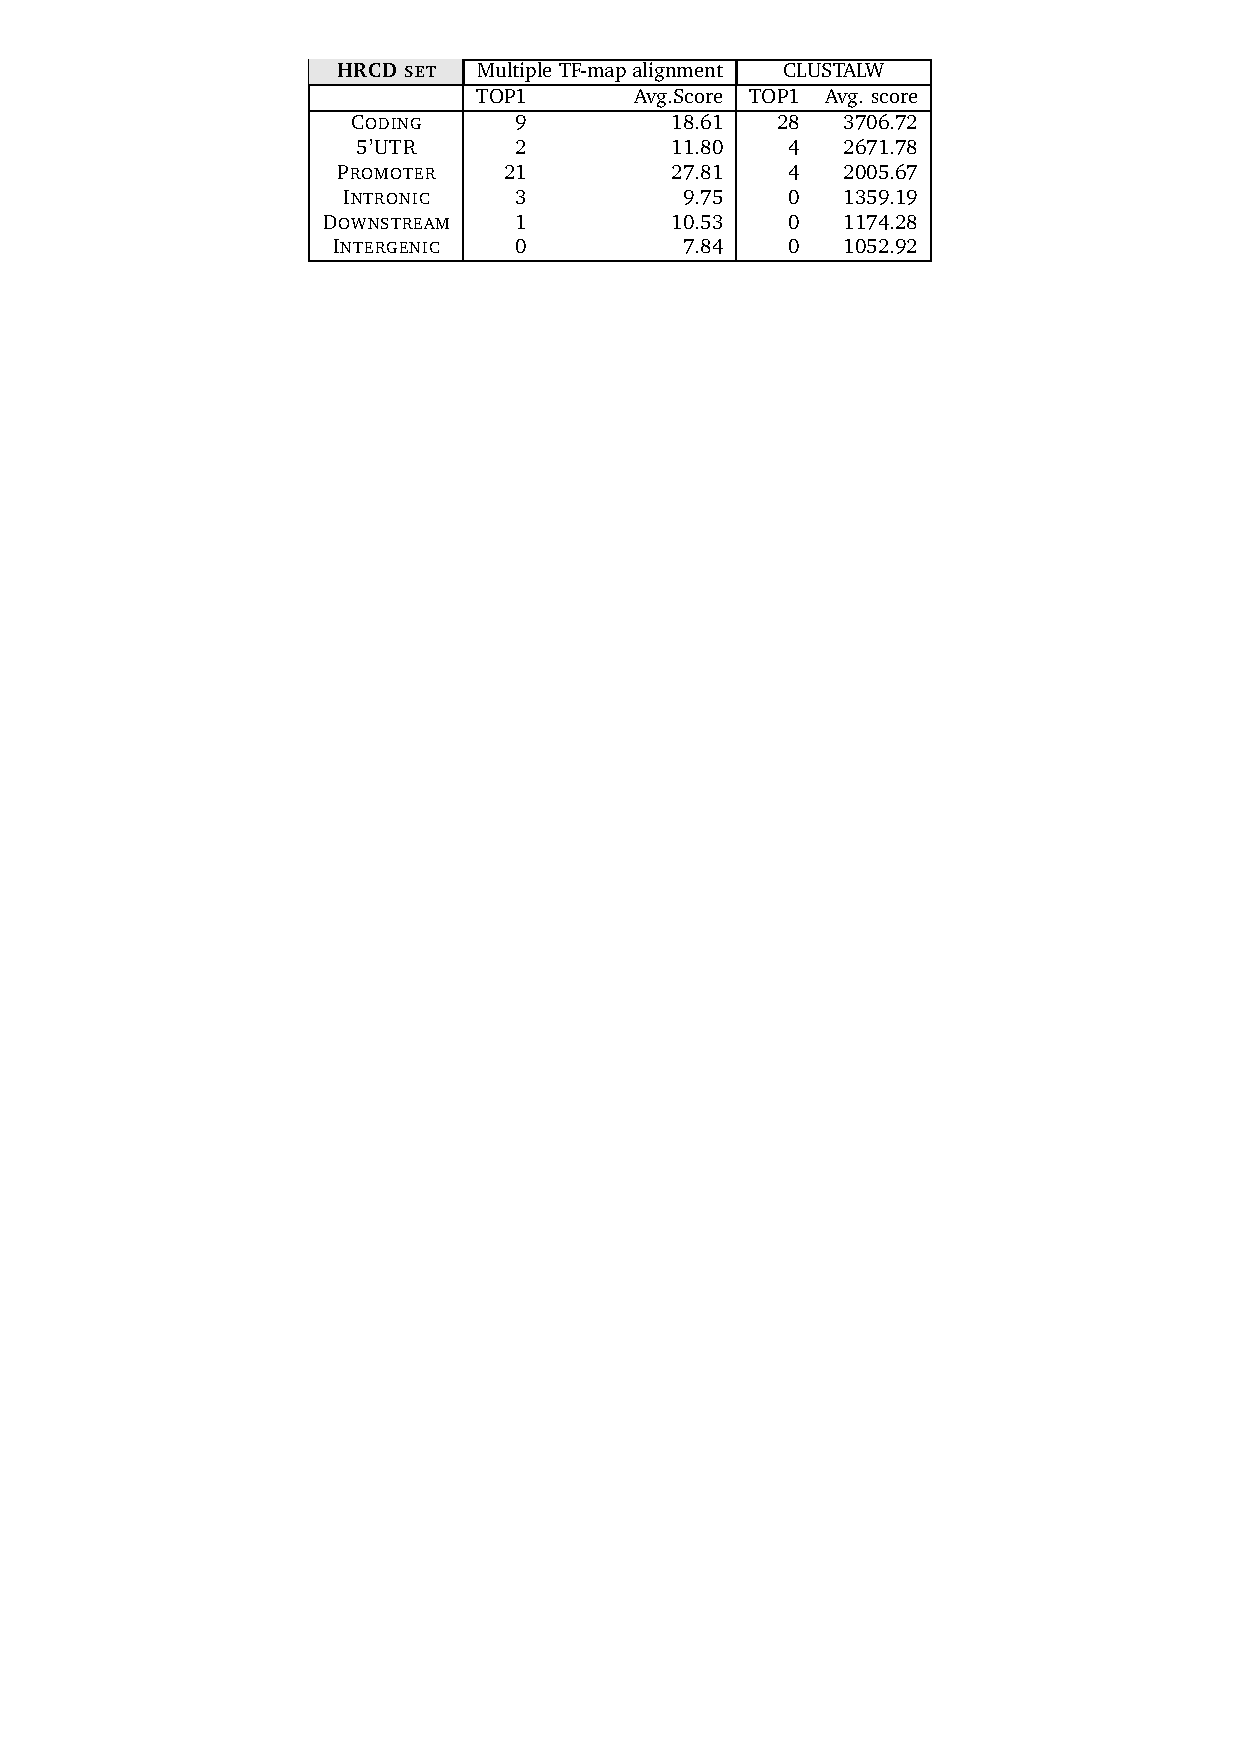
\includegraphics[bb=141 715 449 817,clip]{tables/testregionsM}}
\end{center}
\end{minipage}
\mycaption{tab:testregionsM}% label
          {Results when distinguishing promoters with MMAs}% lof
          {Results when distinguishing promoters with MMAs.}% caption header
          {}
\end{center}
\end{table}

Thus, we can not repeat the training procedure used in \citep{blanco:2006b}
to evaluate the ability of MMA to detect conserved regulatory elements at
larger evolutionary distances --at which the degree of conservation may
be negligible. However, we can use another method, also presented in
\citep{blanco:2006b}, to show that MMAs are much more informative than
primary multiple sequence alignments.

We first have mapped the TFBSs occurrences in the promoter sequences
using the collection of 50 most informatives matrices in \db{JASPAR} 1.0
\citep{sandelin:2004a}, to which we refer as \db{JASPAR$_{TOP50}$} \citep{blanco:2006b}.

Then, we have compared the MMAs obtained in the $200$ nucleotides of the
promoter region of the 36 gene pairs from the \textsc{HRCZ set}, with the
MMAs obtained in fragments of $200$ nucleotides from intergenic ($2,000$
nucleotides upstream of the TSS), 5'UTR (downstream of the TSS), coding
(downstream of the translation start site and considering only coding DNA),
intronic (downstream of the first intron junction), and downstream
(downstream of the transcription termination site) sequences (see
Figure \ref{fig:testregionsM} for a graphical representation of the test).
We have computed the average score of the MMA on each one of the genomic
regions and have identified, for each orthologous set, the genome regions
in which the alignment produces the highest score. We have performed the
same exercise using global pairwise sequence alignments (obtained with
CLUSTALW, \citep{thompson:1994a}).

We have repeated this test using different combinations of parameters.
Systematically, the parameters $\alpha, \lambda$ and $\mu$ were allowed
to independently take values between $0.0$ and $1.0$, in incremental steps
of $0.1$. At the same time, the parameter $\gamma$ (gap penalty) was
tested between $0$ and $-10$. The optimal parameter configuration is 
considered to be that set of parameter values that better discriminate 
between promoters and the rest of genomic regions.

Results appear in Table \ref{tab:testregionsM}. As expected, nucleotide sequence
alignments score the highest in the coding regions (in $28$ out of $36$
cases), followed by the alignments in the 5$^\prime$ UTR regions ($4$
out of $36$) and in the promoters ($4$ out of $36$). The scores of the
sequence alignments show that promoter regions are less conserved than
coding regions, and 5'UTRs. Despite this, the optimal MMA configuration
in the collinear configuration $(\alpha=1,\lambda=0.1,\mu=0.1,\gamma=-2)$
scores the highest in the promoter regions (in $21$ out of $36$, see Table \ref{tab:testregionsM}).
In addition, the average score of map alignments is notably higher than that of
the coding regions. Only in $9$ out of $36$ cases the TF-map alignments score
the highest in coding regions. Interestingly, while intron sequences in the
human-mouse-chicken-zebrafish orthologs are much less conserved than 5'UTRs,
MMAs score the highest in intronic regions in $3$ cases whereas they only
score the best in 5'UTRs in $2$ cases. This is consistent with the fact that
first introns are known to often contain regulatory motifs.

%Shuffle test
Finally, we have also performed a complementary test to measure the 
specificity of the TF-map alignments. As a negative control, we have shuffled 
the orthologous associations in the \textsc{HRCZ set} to construct a pool of 
unrelated human-mouse-chicken-zebrafish $36$ gene entries. Then, the 
corresponding multiple TF-map alignments of these non-orthologous paired
promoters were obtained using the parameters previously optimized.
The TF-map alignments of the unrelated promoters of each entry were 
significantly worse with an average score more than 50\% smaller than 
TF-map alignments that involved ``bona fide'' orthologous promoters. 
For instance, the average score of the TF-map alignments among orthologous 
promoters when using the \db{JASPAR$_{TOP50}$} collection was $27.81$. In contrast, 
the score of the TF-map alignments between non-related promoters was $12.51$. 
The sites in the alignments involving non-orthologous gene promoters may 
hypothetically correspond to general regulatory elements present 
in most core promoters. An alternative, more probable, hypothesis is that they
reflect the poor specificity of most PWMs representing TFBSs.

\subsectionblue{Promoter characterization}

We have selected three examples to show the ability of MMAs to characterize
promoter regions in the absence of sequence conservation. In the three cases, 
we have compared the multiple TF-map aligment against the corresponding multiple 
sequence alignment produced by CLUSTALW, as in the section above. 

All of the cases are graphically represented as pictures in which the
input TF-maps are displayed on the upper part of the picture and the
resulting MMAs are displayed on the lower part of the picture, using the
\prog{gff2ps} program \citep{abril:2000a}.

%%%%
% Figure 13: 
%%%%
\begin{figure}[t!]
\begin{center}
\setlength{\fboxsep}{0pt}
%\fbox{
\incgraph{width=0.9\linewidth}{ps/a00}%}
\mycaption{fig:A00s}% label
          {Multiple promoter characterization}% lof
          {Multiple promoter characterization.}% caption header
          {(Top) \db{JASPAR} predictions and the MMA among the \emph{Actin $\alpha$-cardiac} 
           gene promoters. 
           (Bottom) \db{JASPAR} predictions and the MMA among the \emph{Myoglobin} gene promoters.}
\end{center}
\end{figure}

As it is possible to see, the main effect of the MMA is the
dramatic reduction in the number of predicted TFBSs that typically
result after a PWM-based search (see Figure \ref{fig:A00s} and Figure \ref{fig:MMP13}). 
For instance, we aligned $157$ human sites to $197$ mouse sites, $229$ chicken sites
and $167$ zebrafish sites mapped in the respective Actin $\alpha$-cardiac 
gene promoter orthologs (see next section). The resulting multiple TF-map alignment 
only contained $14$ TFBSs, which approximately represents a 13-fold reduction.
Graphically, this reduction is noticed in the smaller density of aligned sites in 
the resulting MMAs picture.

In addition to this, most aligned sites in the MMAs are concentrated in the 
proximal promoter region of each gene ($200$ nucleotides upstream of the TSS). This gain 
in specificity is not simply due to the selection of an arbitrary set of non-overlapping 
TFBSs, as many experimentally annotated TFBSs on these promoters are successfully covered 
by the MMAs.


\subsubsectionblue{\emph{Actin $\alpha$-cardiac} gene}

Actins are highly conserved proteins that are involved in various types of cell motility.
The alpha actins are found in muscle tissues and are a major constituent of the contractile 
apparatus. The \emph{Actin $\alpha$-cardiac} gene has been identified in many kinds of cells 
including muscle, where it is a major constituent of the thin filament, and platelets.

The promoter of the human and mouse \emph{Actin $\alpha$-cardiac} genes
(ACTC, \genbank{} entries M13483 and M26773) have been extensively characterized by 
experimental means \citep{wasserman:1998a}. In the ABS database \citep{blanco:2006a}, the 
entry $A0028$ informs about the known orthologous binding sites in the respective human 
and mouse promoters ($500$ nucleotides, the position +501 is the TSS).
The human ACTC promoter is constituted of three SRF sites $(+301, +352, +392)$, 
a SP1 site $(+418)$, a MYOD site $(+445)$ and a TATA box $(+469)$.
Using the \refseq{} gene annotations, we have also identified the 
corresponding orthologous promoters in chicken and zebrafish (\refseq{} entries 
NM\_001031229 and NM\_214784).

We have then aligned the four promoters and compared the resulting MMA with the
functional annotations detailed above. In general terms, the multiple TF-map
alignment of the four orthologous promoters of ACTC contains many of the
functional sites in human and mouse, detecting as well the corresponding
orthologs in the other species. The output coverage is, however, smaller 
than $50$\% of the promoter nucleotides.

The MMA of the ACTC promoters is shown in Figure \ref{fig:A00s} (Top). While the region proximal 
to the TSS is not more dense in predicted TFBSs than other regions, most of the 
aligned elements cluster near to the TSS. In addition, the alignment agrees 
well with the functional annotation available in human and mouse, providing
novel orthologous sites in chicken and zebrafish:

\begin{enumerate}
\item
The second SRF binding site is correctly identified in human, mouse and 
also in zebrafish. 
\item
A RREB-1 site that overlaps the SP-1 active site is identified in the MMA. RREB-1
and SP-1 are both members of the zinc finger protein families \citep{vlieghe:2006a}.
\item
A SQUA site that overlaps the third SRF active site is identified in the MMA.
SQUA and SRF are both members of the MADS family \citep{vlieghe:2006a}.
\item
A novel forth SRF binding site is located immediately upstream of the experimental 
first one at the four species. 
\item
The TATA box is correctly detected in human, mouse and zebrafish as well.
\end{enumerate}

No significant conservation among the sequences was, however, detected in the CLUSTALW multiple 
alignment of the four ACTC promoters (data not shown).

\subsubsectionblue{\emph{Myoglobin} gene}

The \emph{Myoglobin} gene is a member of the globin superfamily and is expressed in 
skeletal and cardiac muscles. The encoded protein is a haemoprotein contributing to 
intracellular oxygen storage and transcellular facilitated diffusion of oxygen.

The promoter of the \emph{Myoglobin} gene in human (MB, \genbank{} entry X00371)
and in mouse (\refseq{} entry NM\_013593) have been experimentally characterized
\citep{bassel:1992a,wasserman:1998a}. In the ABS database \citep{blanco:2006a}, the 
entry $A0037$ informs about the known orthologous binding sites in the respective human 
and mouse promoters ($500$ nucleotides, the position +501 is the TSS).
The human MB promoter is constituted of a CCAC box $(+272)$, a MEF-2 site $(+335)$ with two 
surrounding E-boxes $(+326, +348)$ and a TATA box $(+469)$.
Using the \refseq{} gene annotations, we have also identified the 
corresponding orthologous promoters in chicken and zebrafish (\refseq entries 
NM\_203377 and NM\_200586).

We have then aligned the four promoters and compared the resulting MMA with the
functional annotations detailed above. The multiple TF-map
alignment of the four orthologous promoters of MB contains several of the
functional sites in human and mouse, detecting some of the
orthologs in the other two species. The output coverage is again very small.

The MMA of the MB promoters is shown in Figure \ref{fig:A00s} (Bottom). Most of the aligned
elements are present near to the TSS, while this spatial trend is not observable 
at the predictions at each promoter. The alignment also contains several
of the functional human and mouse sites, providing their counterparts in 
chicken and zebrafish:

\begin{enumerate}
\item
A RREB-1 site that overlaps the functional CCAC box is identified in the MMA.
In fact, the RREB-1 matrix consensus in JASPAR represents an A/C rich area that  
contains the CCAC motif \citep{vlieghe:2006a}.
\item
The TATA box is correctly detected in the four species.
\end{enumerate}

The CLUSTALW multiple alignment of the four MP promoters did not reveal any 
significant conservation (data not shown).


\subsubsectionblue{\emph{Collagenase-3} gene (MMP13)}

The two previous examples have been extracted from the \textsc{HRCZ set}. 
We have now focused on another gene with a more complete set of identified
orthologous promoters to test the ability of the MMAs to elucidate high-level
conservation even at more phylogenetically distant sequences.

%%%%
% Figure 14: 
%%%%
\begin{figure}[t!]
\begin{center}
\setlength{\fboxsep}{0pt}
%\fbox{
\incgraph{width=0.825\linewidth}{ps/MMP13}%}
\mycaption{fig:MMP13}% label
          {MMA of the MMP13 promoter in 9 species}% lof
          {MMA of the MMP13 promoter in 9 species.}% caption header
          {(Top) \db{JASPAR} predictions and the resulting multiple TF-map alignment.
           (Bottom) The CLUSTALW multiple sequence alignment of the 9 promoters.}
\end{center}
\end{figure}

The \emph{Collagenase-3} (MMP13) gene is a member of the matrix metalloproteinase
family. MMP13 plays a major role in normal tissue remodeling processes, being
abnormally expressed in breast carcinomas and in cartilage from arthritic 
patients \citep{pendas:1997a}. Many experimental studies have  
confirmed the presence of several functional binding sites for known TFs
in human and mice 
\citep{pendas:1997a,benbow:1997a,jimenez:1999a,sun:2000a,hess:2001a,benderdour:2002a,wu:2002a}.

Here, we have analized the proximal promoter regions of MMP13 in human, chimp, mouse, rat, 
cow, dog, chicken, zebrafish and \emph{Xenopus} (Ort\'in \emph{et al.}, 
personal communication). As the 5'UTR of this gene is very small in most cases, we have 
considered the region $500$ bps immediately upstream the ATG (Translation Start Codon) as 
the proximal promoter.

We performed the multiple TF-map alignment of the nine MMP13 promoters with 
the optimal configuration calculated in the previous section for four species, 
increasing the $\mu$ parameter to $0.75$ to highlight only those regulatory elements 
that can be aligned in similar positions in most promoters. We also performed the 
multiple sequence alignment of the nine promoters with the program CLUSTALW. The MMA and 
the CLUSTALW alignments are both shown in Figure \ref{fig:MMP13}. 

The comparison between the the resulting MMA shown in Figure \ref{fig:MMP13} (Top) and experimental
annotations on MMP13 gene promoter reveals interesting results. Up to four TFBSs 
that have been experimentally reported to be functional in human and mouse
are remarkably included in such a MMA:

\begin{enumerate}
\item
The AML-1 binding site included in the resulting MMA (position 330 in human promoter; 
alternative names: CBFA-1, OSE-2, OSF-2) \citep{pendas:1997a,jimenez:1999a,hess:2001a}.

\item
The FREAC-4 binding site (position 370 in human promoter; alternative names: FREAC, p53) \citep{sun:2000a}. 
\item
The SPI-1 binding site (position 391 in human promoter; alternative names: AP-1, ETS, PEA-3) 
\citep{pendas:1997a,benbow:1997a,wu:2002a}. The SPI-1 transcription factors are distant related 
members of the Ets family \citep{ray:1995a}.

\item
The TCF11-MafG binding site (position 420 in human promoter, alternative names: AP-1)
\citep{pendas:1997a,benbow:1997a,wu:2002a}. The human transcription factor TCF11 
is known to bind to a subclass of AP1-sites \citep{johnsen:1998a}.
\end{enumerate}

We have not only detected the human and mouse experimental binding sites but we have 
also identified with the MMA the putative novel site of each TF in most orthologs 
of the other species, including the most distant ones. The first 
aligned TF in the MMA (FREAC-3), which has not been experimentally detected so 
far, presents a similar positional conservation in all of the orthologs. 
In addition, the resulting phylogenetic tree constructed from the progressive multiple 
TF-map alignment (shown in red, left) correlates well with the real phylogeny of these 
nine species.

Accurate inspection of the the global sequence alignment by CLUSTALW in Figure \ref{fig:MMP13} (Bottom)
only reveals some weak conservation blocks that could partially contain any of the functional 
TFBSs detected by the multiple TF-map alignment. We also tested several configurations of 
CLUSTALW (adjusting the gap open and gap extension penalties). However, we did not found any 
parameter combination that was able to clearly detect all of the four functional sites.

%%%%
% Figure 15: 
%%%%
\begin{figure}[t!]
\begin{center}
\setlength{\fboxsep}{0pt}
%\fbox{
\incgraph{width=0.65\linewidth}{ps/mememma}%}
\mycaption{fig:mememma}% label
          {Using MEME as a mapping function}% lof
          {Using MEME as a mapping function.}% caption header
          {(Top) The MEME motifs and the resulting MMA in the Actin $\alpha$-cardiac orthologous promoters.
           (Bottom) The MEME motifs and the resulting MMA in the Myoglobin orthologous promoters.}
\end{center}
\end{figure}



%%%%%%%%%%%%%%%%%%
%%% References for this chapter
%%% ENCERRAR ENTRE LLAVES PARA EVITAR PROBLEMAS
\bibliographystyle{plainnat}
{\bibliography{sections/bibliography}}
 % Multiple TF-map alignment
    \clearemptydoublepage

    \chapter[Conclusions]{\textbf{C}onclusions}\label{sec:conclusions}

\index{thesis!concl@conclusions}
\lettrine[lines=4,loversize=-0.1,lraise=0.1,lhang=.2]{T}{he TF-map alignments can be very useful} to
efficiently perform searches of promoter elements that might be conserved in different species. In short, 
the research presented here has contributed to improve the computational characterization of gene 
transcription regulatory regions in the following aspects:

\begin{menumerate}
\item
We have designed a new family of algorithms, which are named TF-map alignments or simply 
meta-alignments, to detect conserved high-order configurations of functional elements that do not show 
discernible sequence conservation. The meta-alignment algorithm does not directly 
compare the primary sequences. Instead, the algorithm aligns the map of high-level
elements obtained with an external mapping function over the original sequences, taking 
into account their position, the element class and the mapping score.

\item
We have generalized the pairwise meta-alignment algorithm to deal with multiple maps.
We followed a progressive approach in which the multiple meta-alignment is build up in
a stepwise manner: a first multiple alignment is created with the two most similar maps,
and the rest of maps or groups of maps are then aligned to this initial multiple meta-alignment
following a guide tree.

\item
We have investigated the structure and the shape of the resulting meta-alignments. We have
incorporated some modifications in the basic algorithm in order to detect non-collinear 
configurations in the alignments without additional computational cost.

\item
We have successfully applied the meta-alignment algorithms on the biological problem of 
eukaryotical promoter characterization. First, we have manually curated a collection of
orthologous transcription factor binding sites from the literature, that are experimentally 
verified in human, mouse, rat or chicken. Next, we have trained the meta-alignment program
on a subset of well characterized human-mouse promoters, extracted from this collection.
Then, we have shown the TF-map alignments are more accurate than conventional sequence 
alignment to distinguish pairwise gene co-expression in a large collection of microarray results. 

\item
We have also used the meta-alignment approach to distinguish promoters from other 
gene regions in a set of well characterized human-rodent gene pairs and their corresponding 
orthologs in chicken and zebrafish. In this particular problem, the multiple meta-alignment 
identified correctly most orthologous promoter regions, even when comparing to protein coding
regions that presented a stronger sequence conservation.

\item
We have comprehensively reviewed the topic of sequence alignment, specially focusing on the 
pioneering algorithms that have mostly contributed to the field. In addition, we have also 
contributed to extend our expertise in the areas of computational gene finding and promoter 
characterization, within the field of bioinformatics.
\end{menumerate}

     % Your contribution in short points
    \clearemptydoublepage

    %% Still do not understand quite well why this is not placed properly
    %% between sections and appendices. The hack here is pretty simple
    %% and seems to work, just place those commands before the last section
    %% include.
    %\addtocontents{toc}{\protect\clearpage}%
    %\addtocontents{toc}{\protect\ \protect\vskip 5ex}%
    %\addtocontents{toc}{\protect\noindent%\hspace*{\protect\fill}%
    %                    {APPENDICES}}%
    %\addtocontents{toc}{\protect\vskip 3ex}%
    %%% the following trick seems to fix the above reported behaviour
    %\thispagestyle{empty}
    %\clearemptydoublepage
	%\chapter*{\textcolor{blue}{APPENDICES}}    

%%% BLOCK 4    
\partred{\textbf{A}ppendices}
    \thispagestyle{empty}
    \clearemptydoublepage

%%% APENDICES %%%%%%%%%%%%%%%%%%%%%%%%%%%%%%%%%%%%%%%%%%%%%%%%%%%%%%%%%%%%%%%%%%

\appendix % Start appendices here %
\setcounter{chapter}{0}

    \noappendix{\textit{Curriculum Vitae}}%\label{sec:}

\newcommand{\cab}[1]{\hspace{-0cm}\textcolor{blue}{\rule{3mm}{3mm}{\Huge #1}}}
\newcommand{\subcab}[1]{\textcolor{blue}{{\Large #1}}}

%\begin{center}
%\begin{tabular}{lcr}
%\hspace{-1cm}\bf\it\huge \textcolor{skyblue}{CURRICULUM VITAE} 
%&
%\hspace{2.5cm}
%&
%{\textcolor{skyblue}{\bf\Large Enrique Blanco Garc\'{\i}a}}
%\end{tabular}
%\textcolor{verydarkblue}{Last update: \today}
%\end{center}

%\vspace{-2cm}
%\begin{center}
%\incgraph{width=0.35\linewidth}{ps/WallaceandMe}
%\end{center}
%\vspace{-1cm}
%\vspace{2cm}

%\vspace{-1cm}
%\noindent\cab{  A. PERSONAL DATA}\\
\sectionred*{PERSONAL DATA}

\begin{tabular}{ll}
\textbf{Name}: &  Enrique Blanco Garc\'{\i}a\\
\textbf{Birthplace and birthdate}: &  Barcelona, January 12th. 1976\\
\textbf{Working Address}: &  Centre de Regulaci\'o Gen\`omica\\
 & Passeig de la Barceloneta 37-49\\
 & Barcelona\\
\textbf{Telephone number}: &  +34 93 224 08 91\\
\textbf{E-mail}: & eblanco@imim.es\\
\textbf{Web page:} & http://genome.imim.es/$\sim$eblanco\\[2ex]
\end{tabular}

%\vspace{0.5cm}
%\noindent\cab{   B. ACADEMIC CURRICULUM}
\sectionred*{ACADEMIC CURRICULUM}

\begin{itemize}
\item
\ver{Engineer in Computer Science} (\emph{Ingeniero superior en Inform\'atica}). Facultat 
d\`{ }inform\`atica de Barcelona. Universitat Polit\`ecnica de Catalunya, Spain (June 2000).
[Mark: 7.40/10, PFC: MH]
\item 
\ver{DEA in Algorithmics} (\emph{Diploma de Estudios Avanzados, Research Sufficiency}). 
Departament de Llenguatges i Sistemes Informatics. Facultat d\`{ }inform\`atica de Barcelona. 
Universitat Polit\`ecnica de Catalunya , Spain (June 2002).
\item
\ver{AQU certificate}: Professorat Col.laborador (teaching staff), 25 November 2005.
\end{itemize}

\vspace{0.5cm}
\subcab{Language Skills}

\begin{itemize}
\item English : \ver{Advanced level (Certificat d'\ Aptitud) (Level C)}, Official School of Languages, 
Barcelona (EOIBD), Spain.
\item Italian : \ver{Elementary level (Certificat Elemental) (Level B)}, Official School of Languages, 
Barcelona (EOIBD), Spain.
\item Catalan and Spanish : mother tongues.
\end{itemize}

%\vspace{0.5cm}
%\noindent\cab{   C. RESEARCH CURRICULUM}
\sectionred*{RESEARCH CURRICULUM}

\begin{itemize}
\item 2001 - 2006. PhD student (Software program, Universitat Polit\`ecnica de Catalunya) 
at Genome Informatics Research Lab, IMIM, Barcelona.\\ 
\noindent PhD supervisors:
\begin{itemize}
\item Dr. Xavier Messeguer - peypoch@lsi.upc.edu\\
(Facultat d\`{ }inform\`atica de Barcelona. Universitat Polit\`ecnica de Catalunya) 
\item
Dr. Roderic Guig\'{o} - rguigo@imim.es\\
(Genome Informatics Research Lab, Research Group of Medical Informatics. 
IMIM-UPF-CRG).
\end{itemize}

\item 1999 - 2000. Programmer in Genome Informatics Research Lab, Research Group 
of Medical Informatics, at IMIM, Barcelona.
\end{itemize}

\vspace{0.5cm}
\subcab{Research areas}
\begin{enumerate}
\item Bioinformatics (algorithmics)
\begin{itemize}
\item Sequence analysis
\item Sequence and map alignments
\item Multiple alignments
\item Representation of biological signals
\end{itemize}

\item Bioinformatics (computational biology)
\begin{itemize}
\item Characterization of gene regulatory regions
\item Gene expression
\item Comparative genomics
\item Microarray analysis
\item Computational gene prediction
\end{itemize}

\item Computer Science
\begin{itemize}
\item Algorithmics
\item Artificial intelligence
\item Parallelism and supercomputation
\item Internet aplications
\end{itemize}
\end{enumerate}

\vspace{0.5cm}
\subcab{Computer Skills}
\begin{itemize}
\item
Programming languages: Perl, C, C++, Java, LISP, Pascal, Modula, Ada, PVM, Prolog, GAWK
\item
Document edition: \LaTeX, \texttt{pdflatex}
\item
Web design: XML, HTML, JavaScript, CGI-scripts (web servers), Macromedia Flash, CSSs
\item
Operating systems:  Linux, MAC OS X, Irix, Solaris, Windows 95/98/00/XP
\item
Office: Word, PowerPoint, Excel, Access
\end{itemize}



\vspace{1cm}
\subcab{Publications}

\begin{itemize}
\item
\textbf{E. Blanco}, X. Messeguer, T.F. Smith and R. Guig\'{o}. Transcription Factor Map Alignment of Promoter Regions. \emph{PLOS Computational Biology}, 2(5):e49(2006). 
\item
\textbf{E. Blanco}, D. Farre, M. Alb\`a, X. Messeguer, and R. Guig\'{o}. ABS: a database of Annotated regulatory Binding Sites from orthologous promoters. \emph{Nucleic Acids Research}, 34:D63-D67 (2006). 
\item
\textbf{E. Blanco} and R. Guig\'{o}. Predictive Methods Using DNA Sequences. In A. D. Baxevanis and B. F. Francis Ouellette, chief editors: \emph{Bioinformatics: A Practical Guide to the Analysis of Genes and Proteins, Third Edition}. John Wiley \& Sons Inc., New York (2005).
ISBN: 0-471-47878-4. 

\item
S. Castellano, S.V. Novoselov, G.V. Kryukov, A. Lescure, \textbf{E. Blanco}, A. Krol. V.N. Gladyshev and R. Guig\'{o}. Reconsidering the evolution of eukaryotic selenoproteins: a novel non-mammalian family with scattered phylogenetic distribution. \emph{EMBO reports}, 5(1):71-77 (2004). 

\item 
S. Beltran, \textbf{E. Blanco}, F. Serras, B. Perez-Villamil, R. Guig\'{o}, S. Artavanis-Tsakonas and 
M. Corominas. Microarray analysis of the transcriptional network controlled by the trithorax group 
gene ash2 in Drosophila melanogaster, \emph{PNAS}, 100: 3293-3298, (2003). 

\item
\textbf{E. Blanco}, G. Parra and R. Guig\'{o}. Using geneid to Identify Genes. In A. Baxevanis and D.B. Davidson, chief editors: \emph{Current Protocols in Bioinformatics}. Volume 1, Unit 4.3 (1-26). John Wiley \& Sons Inc., New York, (2002). ISBN: 0-471-25093-7.

\item 
G. Parra, \textbf{E. Blanco}, and R. Guig\'{o}. geneid in Drosophila. \emph
{Genome Research}, 10: 511-515, (2000).
\end{itemize}

\vspace{0.5cm}
\subcab{Posters}
\begin{itemize}
\item
\textbf{E. Blanco}, M. Pignatelli, X. Messeguer and R. Guig\'{o}. 
``Deconstructing the position weight matrices to detect regulatory elements. Systems Biology meeting: global regulation of gene expression''. \emph{Cold Spring Harbor: global regulation of gene expression}. (March 2005, New York, USA). 

\item
\textbf{E. Blanco}, X. Messeguer and R. Guig\'{o}. 
``Novel computational methods to chracterize regulatory regions. Systems Biology meeting: genomic approaches to transcriptional regulation''. \emph{Cold Spring Harbor: genomic approaches to transcriptional regulation}. (March 2004, New York, USA). 

\item
\textbf{E. Blanco}, X. Messeguer and R. Guig\'{o}. 
``Alignment of Promoter Regions by Mapping Nucleotide Sequences into Arrays of Transcription 
Factor Binding Motifs''. \emph{Seventh annual internation conference on computational biology-RECOMB}. (April 2003, Berlin, Germany).

\item
\textbf{E. Blanco}, G. Parra, S. Castellano, J.F. Abril, M. Burset, X. Fustero, X. Messeguer 
and R. Guig\'{o}. ``Gene prediction in the post-genomic era''. \emph{9-th international conference on Intelligent Systems in Molecular Biology}. (July 2001, Copenhaguen, Denmark).

\item J.F. Abril, \textbf{E. Blanco}, M. Burset, S. Castellano, X. Fustero,  G. Parra and  R. Guig\'o; ``Genome Informatics Research Laboratory: Main Research Topics.''{\it I Jornadas de 
Bioinform\'atica} (June 2000, Cartagena, Spain). 
\end{itemize}

\vspace{0.5cm}
\subcab{Grants}
\begin{itemize}
\item
Predoctoral fellowship. Formacion de Personal Investigador (FPI). Ministerio de Educacion y 
Ciencia (Spain), 2001-2004.
\item
Predoctoral fellowship. Institut Municipal d'Investigacio Medica (Spain), 2005-2006.
\end{itemize}

\vspace{0.5cm}
\subcab{Participation in Research Projects}
\begin{itemize}
\item
Plan Nacional I+D (2003-2006), ref. BIO2003-05073, Ministerio de Ciencia
y Tecnologia (Spain). Principal investigator: Dr. R. Guig\'o i Serra.
\item
Plan Nacional I+D (2000-2003), ref. BIO2000-1358-C02-02 Ministerio de Ciencia
y Tecnologia (Spain). Principal investigator: Dr. R. Guig\'o i Serra.
\end{itemize}

%\vspace{0.5cm}
%\noindent\cab{   D. TEACHING CURRICULUM}
\sectionred*{TEACHING CURRICULUM}

\vspace{0.5cm}
\subcab{Topics}

\begin{itemize}
\item Sequence alignment
\item Dynamic programming
\item Data structures
\item Bioinformatics
\item Weight matrices
\item Likelihood ratios
\item Pattern discovery (EM)
\item Computational gene prediction
\item Promoter characterization
\item Genome browsers on internet
\item Artificial neural nets
\item Markov models
\item Hidden Markov models
\item The Human Genome Project
\item DNA computing
\item Introduction to UNIX
\end{itemize}

\vspace{0.5cm}
\subcab{Teaching Activities}\\

\textcolor{blue}{\rule{3mm}{3mm}{\Large $2006$}}

\begin{itemize}
\item Participation in the master \emph{Tecnologie bioinformatiche applicate alla medicina personalizzata} (Genefinding: 
a primer). Consorzio21/Polaris - parco scientifico e tecnologico della Sardegna. Pula (Italy). [Master, 20h]

\item January-March. Participation in the course \emph{Bioinformatica} at Facultat de Ciencies
de la Salut i de la Vida. Universitat Pompeu Fabra. Barcelona (Spain). [University degree, 60h]\\
\end{itemize}

\textcolor{blue}{\rule{3mm}{3mm}{\Large $2005$}}
\begin{itemize}
\item Participation in the course \emph{Bioinformatica} at Facultat de Ciencies
de la Salut i de la Vida. Universitat Pompeu Fabra. Barcelona (Spain). [University degree, 60h]

\item Participation in the Phd course \emph{Eines informatiques per a genetica molecular} 
(Computational Gene Prediction). PhD program in Genetics. Facultat de Biologia. Universitat de 
Barcelona. Barcelona (Spain). [PhD program, 5h]

\item Participation in the summer course \emph{Bioinformatica per a tothom} (Genome analysis). 
Universitat d'Estiu de la Universitat Rovira i Virgili. Reus (Spain). [Summer course, 10h] 

\item Participation in the summer course \emph{Bioinformatica} (Computational Gene Prediction). 
Universidad Complutense de Madrid. Madrid (Spain). [Summer course, 6h] 

\item Participation in the master \emph{Bioinformatics for health sciences} (Introduction to 
the UNIX environment). Universitat Pompeu Fabra. Barcelona (Spain). [Master, 10h]\\
\end{itemize}

\textcolor{blue}{\rule{3mm}{3mm}{\Large $2004$}}
\begin{itemize}
\item Participation in the course \emph{Bioinformatica} at Facultat de Ciencies
de la Salut i de la Vida. Universitat Pompeu Fabra. Barcelona (Spain). [University degree, 60h]

\item Participation in the Phd course \emph{Eines informatiques per a genetica molecular} 
(Computational Gene Prediction). PhD program in Genetics. Facultat de Biologia. Universitat de 
Barcelona. Barcelona (Spain). [PhD program, 5h]

\item Participation in the summer course \emph{Bioinformatica} (Computational Gene Prediction). 
Universidad Complutense de Madrid. Madrid (Spain). [Summer course, 5h]

\item Participation in the master \emph{Bioinformatics for health sciences} (Introduction to 
the UNIX environment). Universitat Pompeu Fabra. Barcelona (Spain). [Master, 10h] 

\item Participation in the workshop on \emph{Computational genome analysis} at Cosmocaixa,
Fundaci\'o La Caixa. Barcelona (Spain). [Workshop, 4h] 

\item Participation in the \emph{Postgraduate programme in Bioinformatics} (Computational Gene 
Prediction). Universidade de Lisboa / Gulbenkian Institute. Lisbon (Portugal). [Master, 40h]\\ 
\end{itemize}

\textcolor{blue}{\rule{3mm}{3mm}{\Large $2003$}}
\begin{itemize}

\item Participation in the course \emph{Bioinformatica} at Facultat de Ciencies
de la Salut i de la Vida. Universitat Pompeu Fabra. Barcelona (Spain). [University degree, 60h]

\item Participation in the Phd course \emph{Eines informatiques per a genetica molecular} 
(Computational Gene Prediction). PhD program in Genetics. Facultat de Biologia. Universitat de 
Barcelona. Barcelona (Spain). [PhD program, 5h]

\item Participation in the master \emph{Bioinformatica y biologia computacional} 
(Computational Gene Prediction). Universidad Complutense de Madrid. Madrid (Spain). [Master, 4h]\\
\end{itemize}

\textcolor{blue}{\rule{3mm}{3mm}{\Large $2002$}}
\begin{itemize}
\item Participation in the course \emph{Bioinformatica} at Facultat de Ciencies
de la Salut i de la Vida. Universitat Pompeu Fabra. Barcelona (Spain). [University degree, 60h]
\item Participation in the course \emph{Bioinformatica} (Genome analysis) at ALMA bioinformatics.
Madrid (Spain). [Course, 8h]\\
\end{itemize}

\textcolor{blue}{\rule{3mm}{3mm}{\Large $2001$}}
\begin{itemize}
\item Participation in the EMBL course \emph{Bioinformatics for comparative and functional 
genomics} (Computational analysis of promoter regions). Universitat Pompeu Fabra. 
Barcelona (Spain). [Course, 2h]\\
\end{itemize}

\textcolor{blue}{\rule{3mm}{3mm}{\Large $2000$}}
\begin{itemize}
\item Participation in the EMB-net course \emph{Bioinformatics} (Computational gene 
identification). Gulbenkian Institute. Lisbon (Portugal). [Course, 20h]\\
\end{itemize}

\vspace{0.5cm}
\subcab{Attended conferences}\\

\begin{itemize}

\item Cold Spring Harbor Labs: global regulation of gene expression. (March 2005, New York, USA). 

\item Cold Spring Harbor Labs: genomic approaches to transcriptional regulation. (March 2004, New York, USA). 

\item IV Jornadas de Bioinform\'atica Espa\~nolas (September 2003, A Coru\~na, Spain). 

\item Seventh annual internation conference on computational biology-RECOMB. (April 2003, Berlin, Germany).

\item Workshop sobre bioinformatica y biologia computacional. Fundacion BBVA. (April 2002, Madrid, Spain).

\item 9-th international conference on Intelligent Systems in Molecular Biology. (July 2001, Copenhaguen, Denmark).

\item I Jornadas de Bioinform\'atica Espa\~nolas (June 2000, Cartagena, Spain). 

\item Jornada Catalana de Supercomputaci\'on. Parque tecnol\'ogico de la Universidad de 
Barcelona (October 1999, Barcelona). 

\item Segunda jornada cient\'ifica sobre an\'alisis computacional de biomol\'eculas. IMIM-UPF (October 1999, Barcelona).
\end{itemize}





              % Your curriculum vitae
    \clearemptydoublepage

    \noappendix{Software}%\label{sec:}

\sectionred*{TF-map alignments}

\begin{mitemize}
\item
\textbf{Programs:} \url{http://genome.imim.es/software/meta/index.html}
\item
\textbf{Web server:} \url{http://genome.imim.es/software/meta/meta.html}
\item
\textbf{Datasets:} \url{http://genome.imim.es/datasets/meta2005/index.html}
\end{mitemize}

\sectionred*{Multiple TF-map alignments}

\begin{mitemize}
\item
\textbf{Programs:} \url{http://genome.imim.es/software/mmeta/index.html}
\item
\textbf{Web server:} \url{http://genome.imim.es/software/mmeta/mmeta.html}
\item
\textbf{Datasets:} \url{http://genome.imim.es/datasets/mmeta2006/index.html}
\end{mitemize}

\sectionred*{The ABS database of annotated promoters} 

\begin{mitemize}
\item
\textbf{Data:}
\url{http://genome.imim.es/datasets/abs2005/index.html}
\item
\textbf{Constructor:}\\ 
\url{http://genome.imim.es/datasets/abs2005/constructor.html}
\item
\textbf{Evaluator:}\\ 
\url{http://genome.imim.es/datasets/abs2005/evaluator.html}
\end{mitemize}


\sectionred*{The \prog{geneid} program} 

\begin{mitemize}
\item
\textbf{Program:} \url{http://genome.imim.es/software/geneid/index.html}
\item
\textbf{Web server:} \url{http://genome.imim.es/software/geneid/geneid.html}
\item
\textbf{Annotations:} \url{http://genome.imim.es/genepredictions/index.html}
\end{mitemize}


        % Software and databases webs
    \clearemptydoublepage

    \noappendix{List of Publications}%\label{sec:}

\sectionred*{Papers}

%\begin{itemize}

\incitem{2006_PLOS}{%
  E. Blanco, X. Messeguer, T.F. Smith and R. Guig\'{o}.\\
  ``Transcription factor map alignment of promoter regions.''\\
  \journal{PLoS Computational Biology}, 2: e49:403--416, 2006.}%

\vspace{0.5cm}

\incitem{2006_NAR}{%
  E. Blanco, D. Farr\'e, M. Alb\`a, X. Messeguer and R. Guig\'o.\\
  ``ABS: a database of Annotated regulatory Binding Sites\\ from orthologous promoters.''\\
  \journal{Nucleic Acids Research}, 34:D63--D67, 2006.}%

\vspace{0.5cm}

\incitem{2004_EMBO}{%
  S. Castellano, S.V. Novoselov, G.V. Kryukov, A. Lescure,\\ E. Blanco, A. Krol. V.N. Gladyshev and R. Guig\'o.\\
  ``Reconsidering the evolution of eukaryotic selenoproteins:\\ a novel non-mammalian family with scattered phylogenetic\\ distribution.''\\
  \journal{EMBO Reports}, 5:71--77, 2004.}%

\vspace{0.5cm}

\incitem{2003_PNAS}{%
   S. Beltran, E. Blanco, F. Serras, B. Perez-Villamil, R. Guig\'{o},\\ S. Artavanis-Tsakonas and M. Corominas.\\
  ``Transcriptional network controlled by the trithorax-group\\ gene ash2 in Drosophila melanogaster.''\\
  \journal{Proc. Nat. Acad. Sci.}, 100:3293--3298, 2003.}%

\vspace{0.5cm}

\incitem{2000_GenRes}{%
   G. Parra, E. Blanco and R. Guig\'{o}.\\
  ``Geneid in Drosophila.''\\
  \journal{Genome Research}, 10:511--515, 2000.}%

%\end{itemize}

\sectionred*{Book Chapters}

\incitem{2005_Baxevanis}{%
  E. Blanco and R. Guig\'{o}.\\
  ``Predictive Methods Using DNA Sequences.''\\
  In A. D. Baxevanis and B. F. Francis Ouellette, chief editors:\\
  \textbf{Bioinformatics: A Practical Guide to the Analysis of Genes\\ and Proteins, Third Edition.}\\
  John Wiley \& Sons Inc., New York, 2005. ISBN: 0--471--47878--4.}%

\vskip 1ex

\incitem{2002_Baxevanis}{%
  E. Blanco, G. Parra and R. Guig\'{o}.\\
  ``Using geneid to Identify Genes.''\\
  In A. D. Baxevanis and D. B. Davison, chief editors:\\
  \textbf{Current Protocols in Bioinformatics. Volume 1.}\\
  John Wiley \& Sons Inc., New York, 2002. ISBN: 0--471--25093--7.}%

\sectionred*{Posters}
%INCLUIR DESPUES EN FORMATO A4 LOS + RELEVANTES

\noindent E. Blanco, M. Pigantelli, X. Messeguer and R. Guig\'{o}.\\
  ``Deconstructing the position weight matrices to detect regulatory elements.''\\
  Global regulation of gene expression, Cold Spring Harbor, USA (2005)
\vskip 1.75ex

\noindent E. Blanco, X. Messeguer and R. Guig\'{o}.\\
  ``Novel computational methods to chracterize regulatory regions.''\\
  Genomic approaches to transcriptional regulation, Cold Spring Harbor, USA (2004)
\vskip 1.75ex

\noindent E. Blanco, X. Messeguer and R. Guig\'{o}.\\
  ``Alignment of promoter regions by mapping nucleotide sequences into arrays\\ of transcription factor binding motifs.''\\
  VII\textsuperscript{\textsl{th}} RECOMB, Berlin, Germany (2003)
\vskip 1.75ex

\noindent E. Blanco, G. Parra, S. Castellano, J.F. Abril, M. Burset,\\ X. Fustero, X. Messeguer and R. Guig\'{o}.\\
  ``Gene Prediction in the Post-Genomic Era.''\\
  IX\textsuperscript{\textsl{th}} ISMB, Copenhagen, Denmark (2001)
\vskip 1.75ex

\noindent J.F. Abril, M. Alb\`{a}, E. Blanco, M. Burset, F. C\^{a}mara, S. Castellano,\\ R. Castelo, O. Gonzalez, G. Parra and R. Guig\'{o}.\\
  ``Understanding the Eukaryotic Genome Sequence.''\\
  Inaugural Symposium of the Center for Genomic Regulation, Barcelona, Spain (2002)
\vskip 1.75ex

\noindent E. Blanco, G. Parra, S. Castellano, J.F. Abril, M. Burset, X. Fustero,\\ X. Messeguer and R. Guig\'{o}.\\
  ``Gene Prediction in the Post-Genomic Era.''\\
  IX\textsuperscript{\textsl{th}} ISMB, Copenhagen, Denmark (2001)
\vskip 1.75ex

\noindent J.F. Abril, E. Blanco, M. Burset, S. Castellano, X. Fustero, G. Parra and R. Guig\'{o}.\\
  ``Genome Informatics Research Laboratory: Main Research Topics.''\\
  I\textsuperscript{\textsl{st}} Jornadas de Bioinform\'{a}tica, Cartagena, Spain (2000)
\vskip 1.75ex


    % List of articles, books and posters
    \clearemptydoublepage

    %%
%% $Id: publications.tex 11 2005-03-29 00:58:58Z jabril $
%%

\noappendix{Publications}%\label{sec:}

\sectionred*{Blanco \emph{et al.}, PLoS Comput Biol 2(5): e49, 2006}

%PLOS editor acceptation letters
%\newpage
%\scalebox{0.85}{
%\begin{minipage}[][][c]{0.95\linewidth}
%\input{plos-letters}
%\end{minipage}}

\newpage
\includepaper{pages={1},noautoscale=true,scale=0.75,
%FULL\includepaper{pages={1-14},noautoscale=true,scale=0.75,
              link,linkname=pap:abs,%
              %addtotoc={},%
              %trim=32 0 50 20,clip,
              offset=20pt -20pt}%26 -28.5
             {width=.95\linewidth}{2006_PLOS} % NAR

\sectionred*{Blanco \emph{et al.}, NAR 34:D63--D67, 2006}

\includepaper{pages={1},noautoscale=true,scale=0.75,
%\includepaper{pages={1-5},noautoscale=true,scale=0.75,
              link,linkname=pap:abs,%
              %addtotoc={},%
              %trim=32 0 50 20,clip,
              offset=20pt -20pt}%26 -28.5
             {width=.95\linewidth}{2006_NAR} % NAR

\sectionred*{Castellano \emph{et al.}, EMBO Reports 5:71--77, 2004}

\includepaper{pages={1},noautoscale=true,scale=0.75,
%FULL\includepaper{pages={1-7},noautoscale=true,scale=0.75,
              link,linkname=pap:abs,%
              %addtotoc={},%
              %trim=32 0 50 20,clip,
              offset=20pt -20pt}%26 -28.5
             {width=.95\linewidth}{2004_EMBO} % EMBO

\sectionred*{Beltran \emph{et al.}, PNAS 100:3293--3298, 2003}

\includepaper{pages={1},noautoscale=true,scale=0.75,
%FULL\includepaper{pages={1-6},noautoscale=true,scale=0.75,
              link,linkname=pap:abs,%
              %addtotoc={},%
              %trim=32 0 50 20,clip,
              offset=20pt -20pt}%26 -28.5
             {width=.95\linewidth}{2003_PNAS} % PNAS

\sectionred*{Parra \emph{et al.}, GenRes 10:511--515, 2000}

\includepaper{pages={1},noautoscale=true,scale=0.75,
%FULL\includepaper{pages={1-5},noautoscale=true,scale=0.75,
              link,linkname=pap:abs,%
              %addtotoc={},%
              %trim=32 0 50 20,clip,
              offset=20pt -20pt}%26 -28.5
             {width=.95\linewidth}{2000_GenRes} % GR

\sectionred*{Blanco and Guig\'o, in Baxevanis and Ouellette, 2005}

\includepaper{pages={3},noautoscale=true,scale=0.75,
%FULL\includepaper{pages={3-29},noautoscale=true,scale=0.75,
              link,linkname=pap:abs,%
              %addtotoc={},%
              %trim=32 0 50 20,clip,
              offset=20pt -20pt}%26 -28.5
              {width=.95\linewidth}{2005_Baxevanis} % BOOK1

\sectionred*{Blanco \emph{et al.}, in Baxevanis \emph{et al.}, 2002}

\includepaper{pages={1},noautoscale=true,scale=0.75,
%FULL\includepaper{pages={1-26},noautoscale=true,scale=0.75,
              link,linkname=pap:abs,%
              %addtotoc={},%
              %trim=32 0 50 20,clip,
              offset=20pt -20pt}%26 -28.5
              {width=.95\linewidth}{2002_Baxevanis} % BOOK1


%


%\end{itemize}


   % Full articles and chapter books
    \clearemptydoublepage

    \noappendix{Posters}%\label{sec:}

\sectionred*{Blanco \emph{et al.}, Cold Spring Harbor, 2005}

\newpage

\begin{center}
\incgraph{width=0.95\linewidth}{ps/CSHL_2005}
\end{center}

\newpage

\sectionred*{Blanco \emph{et al.}, Cold Spring Harbor, 2004}

\newpage

\begin{center}
\incgraph{width=0.95\linewidth}{ps/CSHL_2004}
\end{center}

\newpage

\sectionred*{Blanco \emph{et al.}, RECOMB, 2003}

\newpage

\begin{center}
\incgraph{width=0.95\linewidth}{ps/RECOMB_2003}
\end{center}

\newpage

\sectionred*{Blanco \emph{et al.}, ISMB, 2001}

\newpage

\begin{center}
\incgraph{width=0.95\linewidth}{ps/ISMB_2001}
\end{center}


         % Full posters
    \clearemptydoublepage

    %%
%% $Id: miscellanea.tex 11 2005-03-29 00:58:58Z jabril $
%%

\noappendix{Miscellanea}

This thesis layout is largely derived from the \LaTeX\ template
created by Robert Castelo in 2002\footnote{R. Castelo, April
2002.\newline\hspace*{1cm}''The Discrete Acyclic Digraph Markov Model in Data
Mining''\newline\hspace*{1cm}Faculteit Wiskunde en Informatica, Universiteit
Utrecht}.  His templates were extended by Sergi Castellano and
Gen\'{\i}s Parra for their theses. Josep Francesc Abril substantially 
improved those files, creating an excellent automatical framework that 
produces a variety of different formats and layouts. Here, I provide some 
comments on his version and the modifications I incorporated to, and the 
source code for download.

\index{software!typesetting!latex@\LaTeX|(}%
\sectionred*{Technical comments}

This book was typeset with GNU \prog{emacs} 21.3.1 in \LaTeX\ mode and
converted to PDF with \prog{pdflatex} 3.14159-1.10b (Web2C 7.4.5). All
running on a linux box with Red Hat Fedora Core 2 and kernel
2.6.9-1.6. \LaTeX\ is a document preparation system, powerful, robust
and able to achieve professional results \citep{lamport:1994a}. However,
the learning curve may be stiff. 

The main document, \prog{thesis.tex}, depends on several \LaTeX\
files---including each chapter, the tables and few \ps{} figures---,
but it also depends on other files---such as style files, hacked
\LaTeX\ packages, several bitmaps and the PDF files for the attached
papers. Furthermore, \prog{pdflatex} had to be run several times,
\index{software!typesetting!pdflatex@\prog{pdflatex}}%
together with \BiBTeX\ (to produce the bibliography chapter),
\index{software!typesetting!bibtex@\BiBTeX}%
\prog{makeindex} (to build the index and the web glossary), 
\prog{thumbpdf} (to generate the main PDF document thumbnails),
\index{software!typesetting!thumbpdf@\prog{thumbpdf}}%
and few \perl{} scripts. A \prog{Makefile} was written to automatize
the compilation process of the whole document. In fact, the
\prog{Makefile} was extended to produce four versions of the main
document. The ``\textsl{draft}'' version does not include figures and
the PDF files for the papers, displaying crop marks and boxes
around several elements (such as the area reserved for the
pictures). The ``\textsl{proofs}'', where everything is included but
crop marks and boxes are kept, and different hyperlink types use
different colors. The ``\textsl{pdf}'' version is the electronic
version in which all the hyperlinks are marked in blue color, crop
marks are disabled. Finally, the ``\textsl{press}'' version is very
similar to the ``\textsl{pdf}'' one, currently the only difference
is that all the hyperlinks are black. The \prog{Makefile}
also includes a rule to build the final book ``\textsl{cover}'', which
recycles the \prog{abstract.tex} file and takes some customization
from the same style file as the main \prog{thesis.tex} file.

The compilation of a complete version of this document takes about
\units{600}{seconds}---of course, the ``\textsl{draft}'' version takes much
less---with an AMD Athlon 64 processor 3200+, with \units{512}{KB} of
RAM. This is mainly due to the several steps required to ensure that
every reference, index and so on, is in place. The basic build series
of commands is the following: an initial \prog{pdflatex}, a \BiBTeX\
run to produce the bibliography, a second run of \prog{pdflatex} to
include it, one call to \prog{makeindex} (for the Web Glossary), 
a third run of \prog{pdflatex} to include the
glossary, another call to \prog{makeindex} (to generate the final
index) and to \prog{pdflatex}, then \prog{makeindex} and
\prog{pdflatex} are run again, an extra run of \prog{pdflatex} is
followed by \prog{thumbpdf}, and a final \prog{pdflatex} to obtain the
finished document. If any problem was found, like missing references,
an extra round of \prog{pdflatex}, \BiBTeX\ and \prog{pdflatex} is
performed by the \prog{Makefile}.

Here you can find the version of some of the programs refereed above:
\BiBTeX\ version 0.99c (Web2C 7.4.5), \prog{thumbpdf} version 3.2
(2002/05/26), and \prog{makeindex} version 2.14 (2002/10/02).


\sectionred*{\LaTeX\ Packages}

As there are four versions of the document, the \prog{ifthen} package was
used to define version specific parameters, as well as to include
different files. The package \prog{geometry} facilitates the
definition of the page layout. The current document original dimensions
for both, the electronic and printed versions, are \units{170}{mm}
width by \units{240}{mm} height.  The ``\textsl{cover}'' requires
\prog{calc} to calculate automatically the total width for the page
layout, which includes the front and the back covers and the spine
width. The main document basic font size is the default value for the
``\texttt{book}'' document class, \units{10}{pt}.

The \prog{crop} package is usefull to define the trimming marks for
the ``\textsl{draft}'' and ``\textsl{proofs}'' versions of this
document. It distinguishes between the logical page, the page sizes
defined by the user, and the physical page, the page size for the
hardcopy. The \prog{layout} package is used in the ``\textsl{draft}''
version to show on the first page the \LaTeX\ variable settings
controlling the page layout. Another useful package has been
\prog{nextpage}, which provides additional
``\prog{clear{\ldots}page}'' commands that ensure to get empty even
pages at the end of chapters---and of course, to ensure that all
chapters begin at odd pages---, even with automatically generated
sections like the Bibliography and the Index.

The \prog{babel} package provides a set of options that allow the user
to choose the language(s) in which the document will be typeset, for
instance language-specific hyphenation patterns. The default language
was set to ``\texttt{english}'', while ``\texttt{catalan}'' and
``\texttt{spanish}'' were also loaded for using them for the
corresponding translations of the \textsc{Abstract}.

When working with \prog{pdflatex} there are three unvaluable packages:
\prog{pdfpages}, which makes it easy to embed external PDF documents,
such as the attached publications;
\prog{thumbpdf}, it must be included in files for which a user wants
to generate thumbnails (which are created by the \prog{thumbpdf}
program); and \prog{hyperref}, which extends the functionality of all
the \LaTeX{} cross-referencing commands to produce \prog{special}
commands which a driver can turn into hypertext links.  To protect URL
characters we must load the \prog{url} package, unless we have already provided
\prog{hyperref}. This package has its own version of the \prog{url}
macro, enhanced to provide clickable URLs.

To include \ps{} figures one needs \prog{graphics} and/or
\prog{graphicx}. Those packages are modified by
\prog{pdflatex} so that they are able to include bitmaps
(PNGs, JPEGs, and so on) and PDF files into the document. \prog{color}
facilitates the specification of user-defined colors (such as the
cover green shades). Figures generated with \LaTeX\ can use any of the
following packages: \prog{pstricks}, \prog{pstcol}, \prog{multido}.

The bibliography was produced with \BiBTeX. The package \prog{natbib}
(NATural sciences BIBliography) provides both author-year and
numerical citations; it makes possible to define different
citation styles. We have set the following options:
``\texttt{round}'', to put citations within parenthesis;
``\texttt{colon}'', to separate multiple citations with colons;
``\texttt{authoryear}'' to show author and year citations (instead of
numerical citations); and the option ``\texttt{sectionbib}'' to use
the package \prog{chapterbib}. The style ``\texttt{plainnat}'' was then applied
to format the bibliography. The package \prog{chapterbib} allows to include
a bibliography for each chapter. The package \prog{minitoc} creates
a mini table of contents for each chapter as well. 

\prog{makeidx} provides the macros required to make a subject
index. To show the capital letter section headings, few variables were
redefined on an auxiliary file (\prog{header.ist}).
One glossary was generated for this document: the web references. 
The package \prog{glossary} allowed us to customize the format of this 
section.

We also defined a style file named \prog{mythesis.sty}. It loads the
following font packages: \prog{fontenc} (with ``\texttt{T1}'' option),
to set extended font encoding (accents and so on); \prog{textcomp}, to
include some extra symbols, such as the Euro symbol for instance;
\prog{pifont}, for \textsc{Symbol} and \textsc{Zapf Dingbats} fonts;
\prog{charter}, with which roman family is set to \textsc{BitStream-Charter}; 
\prog{helvet}, with which sans-serif family is set to \textsc{Helvetica}; 
\prog{euler}, with which formulas are set to \textsc{Euler}; 
and \prog{courier}, to set typewriter family to \textsc{Courier}. 
Other packages that were loaded are: \prog{fancyhdr}, to produce nice
headings; \prog{fancyvrb}, to extend the \prog{verbatim} environment;
\prog{comment}, to hide parts of the original \LaTeX\ files;
\prog{rotating}, to rotate boxes of text; and \prog{multirow}, to get
multirow cells within the \prog{tabular} environment.
%; and \prog{multicol} 
\index{software!typesetting!latex@\LaTeX|)}%


\sectionred*{Getting the template files}

You are free to copy, modify and distribute the template files of this
thesis, under the terms of the GNU Free Documentation License as
published by the Free Software Foundation.  Any script bundled in this
distribution, including the \prog{Makefile}, is under the terms of the
GNU General Public License.\index{GNU-GPL} The template for this thesis
as well as the DVD related files are available from:

\centerline{\url{http://genome.imim.es/~eblanco/MyThesis/}}


%%%%%%%%%%%%%%%%%%
%%% References for this chapter
%%% ENCERRAR ENTRE LLAVES PARA EVITAR PROBLEMAS
\bibliographystyle{plainnat}
{\bibliography{sections/bibliography}}

     % Technical stuff about LaTeX
    \clearemptydoublepage              % Make others' life easier by sharing!!!

%%% BACKMATTER %%%%%%%%%%%%%%%%%%%%%%%%%%%%%%%%%%%%%%%%%%%%%%%%%%%%%%%%%%%%%%%%%

\backmatter

%%% Web Site definitions
    \phantomsection % fixes the link anchor
    \renewcommand{\glossaryname}{WebSite References}%
    \renewcommand{\glossarypreamble}%
                 {\label{sec:webrefs}%
                  \addappendix{\glossaryname}%
                 }% glossarypreamble
    \renewcommand{\glossarypostamble}{}%
    \renewcommand{\gloitem}[1]{\item[\avantgarbold{}#1]\mbox{}\par}
    \printweblink                          % Print URLs Index
    \clearemptydoublepage

%%% Subject Index
    \renewcommand{\indexname}{Index}%
    \phantomsection % fixes the link anchor
    \addappendix{\indexname}%
    \printindex  % Print Subject Index
    \clearemptydoublepage

%%% CLOSING NICETIES %%%%%%%%%%%%%%%%%%%%%%%%%%%%%%%%%%%%%%%%%%%%%%%%%%%%%%%%%%%

    \phantomsection % fixes the link anchor
    %%
%% $Id: notes.tex 11 2005-03-29 00:58:58Z jabril $
%%

\chapter*{\textcolor{blue}{Notes}}\markboth{NOTES}{NOTES}

\ \\

\newpage

\ \\

\newpage

\ \\

\newpage

\ \\

\newpage

\ \\

\newpage

               % Courtesy blank pages

    %%
%% $Id: series.tex 11 2005-03-29 00:58:58Z jabril $
%%

\thispagestyle{empty}

\noindent
\textcolor{blue}{{\avantgarboldlarge Titles in the GBL Dissertation Series}}\label{gblseries}

\vspace{1cm}

\small

\begin{tabular}{rl}
\textbf{2002-01} & Mois\'es Burset.\\ 
 & \emph{Estudi computacional de l'especificacio\hspace{-0.6ex}' dels llocs d'splicing.}\\
 &        [Computational analysis of the splice sites definition.]\\
 & Departament de Gen\`{e}tica,
   Universitat de Barcelona. \\

& \\ % empty line between different years

\textbf{2004-01} & Sergi Castellano.\\
 & \emph{Towards the characterization of the eukaryotic selenoproteome:
           a computational approach.} \\
 & Departament de Ci\`{e}ncies Experimentals i de la Salut,
   Universitat Pompeu Fabra. \\

& \\ % empty line between different years

\textbf{2004-02} & Gen\'{\i}s Parra.\\
 & \emph{Computational identification of genes:
           ``ab initio'' and comparative approaches.} \\
 & Departament de Ci\`{e}ncies Experimentals i de la Salut,
   Universitat Pompeu Fabra. \\

& \\ % empty line between different years

\textbf{2005-01} & Josep F. Abril.\\
 & \emph{{Comparative Analysis of Eukaryotic Gene Sequence Features.}} \\
 & Departament de Ci\`{e}ncies Experimentals i de la Salut,
   Universitat Pompeu Fabra. \\

& \\ % empty line between different years

\textbf{2006-01} & Enrique Blanco.\\
 & \emph{{\thytitle}.} \\
 & Departament de Llenguatges i Sistemes Inform\`atics,
   Universitat Polit\`ecnica de Catalunya. \\

\end{tabular}

\vfill
              % Thesis series in the lab

%% BACK COVER
\newpage%
\pagestyle{empty}\hspace{1ex}\\%
\newpage%
\thispagestyle{empty}%
\makebgpage{sections/bookback}{1.5}%


\end{document}

%%% Congratulations, you made it!!! Look for a postdoc now!!!

%%%%%%%%%%%%%%%%%%%%%%%%%%%%%%%%%%%%%%%%%%%%%%%%%%%%%%%%%%%%%%%%%%%%%%%%%%%%%%%%
%        1         2         3         4         5         6         7         8
%2345678901234567890123456789012345678901234567890123456789012345678901234567890
%%%%%%%%%%%%%%%%%%%%%%%%%%%%%%%%%%%%%%%%%%%%%%%%%%%%%%%%%%%%%%%%%%%%%%%%%%%%%%%%

%%%%%%%%%%%%%%%%%%%%%%%%%%%%%%%%%%%%% EOF %%%%%%%%%%%%%%%%%%%%%%%%%%%%%%%%%%%%%%
